\documentclass[twoside]{book}

% Packages required by doxygen
\usepackage{fixltx2e}
\usepackage{calc}
\usepackage{doxygen}
\usepackage[export]{adjustbox} % also loads graphicx
\usepackage{graphicx}
\usepackage[utf8]{inputenc}
\usepackage{makeidx}
\usepackage{multicol}
\usepackage{multirow}
\PassOptionsToPackage{warn}{textcomp}
\usepackage{textcomp}
\usepackage[nointegrals]{wasysym}
\usepackage[table]{xcolor}

% Font selection
\usepackage[T1]{fontenc}
\usepackage[scaled=.90]{helvet}
\usepackage{courier}
\usepackage{amssymb}
\usepackage{sectsty}
\renewcommand{\familydefault}{\sfdefault}
\allsectionsfont{%
  \fontseries{bc}\selectfont%
  \color{darkgray}%
}
\renewcommand{\DoxyLabelFont}{%
  \fontseries{bc}\selectfont%
  \color{darkgray}%
}
\newcommand{\+}{\discretionary{\mbox{\scriptsize$\hookleftarrow$}}{}{}}

% Page & text layout
\usepackage{geometry}
\geometry{%
  a4paper,%
  top=2.5cm,%
  bottom=2.5cm,%
  left=2.5cm,%
  right=2.5cm%
}
\tolerance=750
\hfuzz=15pt
\hbadness=750
\setlength{\emergencystretch}{15pt}
\setlength{\parindent}{0cm}
\setlength{\parskip}{3ex plus 2ex minus 2ex}
\makeatletter
\renewcommand{\paragraph}{%
  \@startsection{paragraph}{4}{0ex}{-1.0ex}{1.0ex}{%
    \normalfont\normalsize\bfseries\SS@parafont%
  }%
}
\renewcommand{\subparagraph}{%
  \@startsection{subparagraph}{5}{0ex}{-1.0ex}{1.0ex}{%
    \normalfont\normalsize\bfseries\SS@subparafont%
  }%
}
\makeatother

% Headers & footers
\usepackage{fancyhdr}
\pagestyle{fancyplain}
\fancyhead[LE]{\fancyplain{}{\bfseries\thepage}}
\fancyhead[CE]{\fancyplain{}{}}
\fancyhead[RE]{\fancyplain{}{\bfseries\leftmark}}
\fancyhead[LO]{\fancyplain{}{\bfseries\rightmark}}
\fancyhead[CO]{\fancyplain{}{}}
\fancyhead[RO]{\fancyplain{}{\bfseries\thepage}}
\fancyfoot[LE]{\fancyplain{}{}}
\fancyfoot[CE]{\fancyplain{}{}}
\fancyfoot[RE]{\fancyplain{}{\bfseries\scriptsize Generated by Doxygen }}
\fancyfoot[LO]{\fancyplain{}{\bfseries\scriptsize Generated by Doxygen }}
\fancyfoot[CO]{\fancyplain{}{}}
\fancyfoot[RO]{\fancyplain{}{}}
\renewcommand{\footrulewidth}{0.4pt}
\renewcommand{\chaptermark}[1]{%
  \markboth{#1}{}%
}
\renewcommand{\sectionmark}[1]{%
  \markright{\thesection\ #1}%
}

% Indices & bibliography
\usepackage{natbib}
\usepackage[titles]{tocloft}
\setcounter{tocdepth}{3}
\setcounter{secnumdepth}{5}
\makeindex

% Hyperlinks (required, but should be loaded last)
\usepackage{ifpdf}
\ifpdf
  \usepackage[pdftex,pagebackref=true]{hyperref}
\else
  \usepackage[ps2pdf,pagebackref=true]{hyperref}
\fi
\hypersetup{%
  colorlinks=true,%
  linkcolor=blue,%
  citecolor=blue,%
  unicode%
}

% Custom commands
\newcommand{\clearemptydoublepage}{%
  \newpage{\pagestyle{empty}\cleardoublepage}%
}

\usepackage{caption}
\captionsetup{labelsep=space,justification=centering,font={bf},singlelinecheck=off,skip=4pt,position=top}

%===== C O N T E N T S =====

\begin{document}

% Titlepage & ToC
\hypersetup{pageanchor=false,
             bookmarksnumbered=true,
             pdfencoding=unicode
            }
\pagenumbering{alph}
\begin{titlepage}
\vspace*{7cm}
\begin{center}%
{\Large Mason }\\
\vspace*{1cm}
{\large Generated by Doxygen 1.8.12}\\
\end{center}
\end{titlepage}
\clearemptydoublepage
\pagenumbering{roman}
\tableofcontents
\clearemptydoublepage
\pagenumbering{arabic}
\hypersetup{pageanchor=true}

%--- Begin generated contents ---
\chapter{Namespace Index}
\section{Namespace List}
Here is a list of all namespaces with brief descriptions\+:\begin{DoxyCompactList}
\item\contentsline{section}{\hyperlink{namespace_mason}{Mason} }{\pageref{namespace_mason}}{}
\item\contentsline{section}{\hyperlink{namespacepicojson}{picojson} }{\pageref{namespacepicojson}}{}
\item\contentsline{section}{\hyperlink{namespace_s_r_e}{S\+RE} }{\pageref{namespace_s_r_e}}{}
\item\contentsline{section}{\hyperlink{namespacestd}{std} }{\pageref{namespacestd}}{}
\end{DoxyCompactList}

\chapter{Hierarchical Index}
\section{Class Hierarchy}
This inheritance list is sorted roughly, but not completely, alphabetically\+:\begin{DoxyCompactList}
\item \contentsline{section}{picojson\+:\+:value\+:\+:\+\_\+storage}{\pageref{unionpicojson_1_1value_1_1__storage}}{}
\item \contentsline{section}{Mason\+:\+:Audio\+Descriptor}{\pageref{class_mason_1_1_audio_descriptor}}{}
\item \contentsline{section}{Mason\+:\+:Audio\+Manager}{\pageref{class_mason_1_1_audio_manager}}{}
\item b2\+Contact\+Listener\begin{DoxyCompactList}
\item \contentsline{section}{Mason\+:\+:Collision\+Listener}{\pageref{class_mason_1_1_collision_listener}}{}
\end{DoxyCompactList}
\item b2\+Draw\begin{DoxyCompactList}
\item \contentsline{section}{S\+R\+E\+Debug\+Draw}{\pageref{class_s_r_e_debug_draw}}{}
\end{DoxyCompactList}
\item \contentsline{section}{Mason\+:\+:Camera\+Descriptor}{\pageref{class_mason_1_1_camera_descriptor}}{}
\item \contentsline{section}{Mason\+:\+:Component}{\pageref{class_mason_1_1_component}}{}
\begin{DoxyCompactList}
\item \contentsline{section}{Mason\+:\+:Audio}{\pageref{class_mason_1_1_audio}}{}
\item \contentsline{section}{Mason\+:\+:Collider2D}{\pageref{class_mason_1_1_collider2_d}}{}
\begin{DoxyCompactList}
\item \contentsline{section}{Mason\+:\+:Box\+Collider2D}{\pageref{class_mason_1_1_box_collider2_d}}{}
\item \contentsline{section}{Mason\+:\+:Circle\+Collider2D}{\pageref{class_mason_1_1_circle_collider2_d}}{}
\end{DoxyCompactList}
\item \contentsline{section}{Mason\+:\+:Particle\+Emitter}{\pageref{class_mason_1_1_particle_emitter}}{}
\item \contentsline{section}{Mason\+:\+:Physics\+Body2D}{\pageref{class_mason_1_1_physics_body2_d}}{}
\item \contentsline{section}{Mason\+:\+:Rendering}{\pageref{class_mason_1_1_rendering}}{}
\item \contentsline{section}{Mason\+:\+:Script}{\pageref{class_mason_1_1_script}}{}
\item \contentsline{section}{Mason\+:\+:Sprite\+Renderer}{\pageref{class_mason_1_1_sprite_renderer}}{}
\item \contentsline{section}{Mason\+:\+:Transform}{\pageref{class_mason_1_1_transform}}{}
\begin{DoxyCompactList}
\item \contentsline{section}{Mason\+:\+:Camera}{\pageref{class_mason_1_1_camera}}{}
\end{DoxyCompactList}
\end{DoxyCompactList}
\item \contentsline{section}{Mason\+:\+:Config}{\pageref{class_mason_1_1_config}}{}
\item \contentsline{section}{picojson\+:\+:default\+\_\+parse\+\_\+context}{\pageref{classpicojson_1_1default__parse__context}}{}
\item \contentsline{section}{picojson\+:\+:deny\+\_\+parse\+\_\+context}{\pageref{classpicojson_1_1deny__parse__context}}{}
\item \contentsline{section}{picojson\+:\+:null\+\_\+parse\+\_\+context\+:\+:dummy\+\_\+str}{\pageref{structpicojson_1_1null__parse__context_1_1dummy__str}}{}
\item \contentsline{section}{Mason\+:\+:Engine}{\pageref{class_mason_1_1_engine}}{}
\item \contentsline{section}{Mason\+:\+:Game\+Object}{\pageref{class_mason_1_1_game_object}}{}
\item \contentsline{section}{Mason\+:\+:Game\+Object\+Descriptor}{\pageref{class_mason_1_1_game_object_descriptor}}{}
\item \contentsline{section}{picojson\+:\+:input$<$ Iter $>$}{\pageref{classpicojson_1_1input}}{}
\item \contentsline{section}{Mason\+:\+:Input\+Manager}{\pageref{class_mason_1_1_input_manager}}{}
\item \contentsline{section}{picojson\+:\+:last\+\_\+error\+\_\+t$<$ T $>$}{\pageref{structpicojson_1_1last__error__t}}{}
\item \contentsline{section}{Mason\+:\+:Leak\+Detection}{\pageref{class_mason_1_1_leak_detection}}{}
\item \contentsline{section}{Mason\+:\+:Mesh\+Descriptor}{\pageref{class_mason_1_1_mesh_descriptor}}{}
\item \contentsline{section}{picojson\+:\+:null}{\pageref{structpicojson_1_1null}}{}
\item \contentsline{section}{picojson\+:\+:null\+\_\+parse\+\_\+context}{\pageref{classpicojson_1_1null__parse__context}}{}
\item \contentsline{section}{Mason\+:\+:Particle\+Descriptor}{\pageref{class_mason_1_1_particle_descriptor}}{}
\item \contentsline{section}{Mason\+:\+:Particle\+Emitter\+Config}{\pageref{struct_mason_1_1_particle_emitter_config}}{}
\item \contentsline{section}{Mason\+:\+:Physics}{\pageref{class_mason_1_1_physics}}{}
\item \contentsline{section}{Mason\+:\+:Scene}{\pageref{class_mason_1_1_scene}}{}
\item \contentsline{section}{Mason\+:\+:Scene\+Parser}{\pageref{class_mason_1_1_scene_parser}}{}
\item \contentsline{section}{picojson\+:\+:serialize\+\_\+str\+\_\+char$<$ Iter $>$}{\pageref{structpicojson_1_1serialize__str__char}}{}
\item \contentsline{section}{Mason\+:\+:Sprite}{\pageref{class_mason_1_1_sprite}}{}
\item \contentsline{section}{Mason\+:\+:Sprite\+Atlas}{\pageref{class_mason_1_1_sprite_atlas}}{}
\item \contentsline{section}{Mason\+:\+:Sprite\+Descriptor}{\pageref{class_mason_1_1_sprite_descriptor}}{}
\item \contentsline{section}{Mason\+:\+:Time}{\pageref{class_mason_1_1_time}}{}
\item \contentsline{section}{Mason\+:\+:Transform\+Descriptor}{\pageref{class_mason_1_1_transform_descriptor}}{}
\item \contentsline{section}{picojson\+:\+:value}{\pageref{classpicojson_1_1value}}{}
\end{DoxyCompactList}

\chapter{Class Index}
\section{Class List}
Here are the classes, structs, unions and interfaces with brief descriptions\+:\begin{DoxyCompactList}
\item\contentsline{section}{\hyperlink{unionpicojson_1_1value_1_1__storage}{picojson\+::value\+::\+\_\+storage} }{\pageref{unionpicojson_1_1value_1_1__storage}}{}
\item\contentsline{section}{\hyperlink{class_mason_1_1_audio}{Mason\+::\+Audio} }{\pageref{class_mason_1_1_audio}}{}
\item\contentsline{section}{\hyperlink{class_mason_1_1_audio_descriptor}{Mason\+::\+Audio\+Descriptor} }{\pageref{class_mason_1_1_audio_descriptor}}{}
\item\contentsline{section}{\hyperlink{class_mason_1_1_audio_manager}{Mason\+::\+Audio\+Manager} }{\pageref{class_mason_1_1_audio_manager}}{}
\item\contentsline{section}{\hyperlink{class_mason_1_1_box_collider2_d}{Mason\+::\+Box\+Collider2D} }{\pageref{class_mason_1_1_box_collider2_d}}{}
\item\contentsline{section}{\hyperlink{class_mason_1_1_camera}{Mason\+::\+Camera} }{\pageref{class_mason_1_1_camera}}{}
\item\contentsline{section}{\hyperlink{class_mason_1_1_camera_descriptor}{Mason\+::\+Camera\+Descriptor} }{\pageref{class_mason_1_1_camera_descriptor}}{}
\item\contentsline{section}{\hyperlink{class_mason_1_1_circle_collider2_d}{Mason\+::\+Circle\+Collider2D} }{\pageref{class_mason_1_1_circle_collider2_d}}{}
\item\contentsline{section}{\hyperlink{class_mason_1_1_collider2_d}{Mason\+::\+Collider2D} }{\pageref{class_mason_1_1_collider2_d}}{}
\item\contentsline{section}{\hyperlink{class_mason_1_1_collision_listener}{Mason\+::\+Collision\+Listener} }{\pageref{class_mason_1_1_collision_listener}}{}
\item\contentsline{section}{\hyperlink{class_mason_1_1_component}{Mason\+::\+Component} }{\pageref{class_mason_1_1_component}}{}
\item\contentsline{section}{\hyperlink{class_mason_1_1_config}{Mason\+::\+Config} }{\pageref{class_mason_1_1_config}}{}
\item\contentsline{section}{\hyperlink{classpicojson_1_1default__parse__context}{picojson\+::default\+\_\+parse\+\_\+context} }{\pageref{classpicojson_1_1default__parse__context}}{}
\item\contentsline{section}{\hyperlink{classpicojson_1_1deny__parse__context}{picojson\+::deny\+\_\+parse\+\_\+context} }{\pageref{classpicojson_1_1deny__parse__context}}{}
\item\contentsline{section}{\hyperlink{structpicojson_1_1null__parse__context_1_1dummy__str}{picojson\+::null\+\_\+parse\+\_\+context\+::dummy\+\_\+str} }{\pageref{structpicojson_1_1null__parse__context_1_1dummy__str}}{}
\item\contentsline{section}{\hyperlink{class_mason_1_1_engine}{Mason\+::\+Engine} \\*Brief about the engine }{\pageref{class_mason_1_1_engine}}{}
\item\contentsline{section}{\hyperlink{class_mason_1_1_game_object}{Mason\+::\+Game\+Object} }{\pageref{class_mason_1_1_game_object}}{}
\item\contentsline{section}{\hyperlink{class_mason_1_1_game_object_descriptor}{Mason\+::\+Game\+Object\+Descriptor} }{\pageref{class_mason_1_1_game_object_descriptor}}{}
\item\contentsline{section}{\hyperlink{classpicojson_1_1input}{picojson\+::input$<$ Iter $>$} }{\pageref{classpicojson_1_1input}}{}
\item\contentsline{section}{\hyperlink{class_mason_1_1_input_manager}{Mason\+::\+Input\+Manager} }{\pageref{class_mason_1_1_input_manager}}{}
\item\contentsline{section}{\hyperlink{structpicojson_1_1last__error__t}{picojson\+::last\+\_\+error\+\_\+t$<$ T $>$} }{\pageref{structpicojson_1_1last__error__t}}{}
\item\contentsline{section}{\hyperlink{class_mason_1_1_leak_detection}{Mason\+::\+Leak\+Detection} }{\pageref{class_mason_1_1_leak_detection}}{}
\item\contentsline{section}{\hyperlink{class_mason_1_1_mesh_descriptor}{Mason\+::\+Mesh\+Descriptor} }{\pageref{class_mason_1_1_mesh_descriptor}}{}
\item\contentsline{section}{\hyperlink{structpicojson_1_1null}{picojson\+::null} }{\pageref{structpicojson_1_1null}}{}
\item\contentsline{section}{\hyperlink{classpicojson_1_1null__parse__context}{picojson\+::null\+\_\+parse\+\_\+context} }{\pageref{classpicojson_1_1null__parse__context}}{}
\item\contentsline{section}{\hyperlink{class_mason_1_1_particle_descriptor}{Mason\+::\+Particle\+Descriptor} }{\pageref{class_mason_1_1_particle_descriptor}}{}
\item\contentsline{section}{\hyperlink{class_mason_1_1_particle_emitter}{Mason\+::\+Particle\+Emitter} }{\pageref{class_mason_1_1_particle_emitter}}{}
\item\contentsline{section}{\hyperlink{struct_mason_1_1_particle_emitter_config}{Mason\+::\+Particle\+Emitter\+Config} }{\pageref{struct_mason_1_1_particle_emitter_config}}{}
\item\contentsline{section}{\hyperlink{class_mason_1_1_physics}{Mason\+::\+Physics} }{\pageref{class_mason_1_1_physics}}{}
\item\contentsline{section}{\hyperlink{class_mason_1_1_physics_body2_d}{Mason\+::\+Physics\+Body2D} }{\pageref{class_mason_1_1_physics_body2_d}}{}
\item\contentsline{section}{\hyperlink{class_mason_1_1_rendering}{Mason\+::\+Rendering} }{\pageref{class_mason_1_1_rendering}}{}
\item\contentsline{section}{\hyperlink{class_mason_1_1_scene}{Mason\+::\+Scene} }{\pageref{class_mason_1_1_scene}}{}
\item\contentsline{section}{\hyperlink{class_mason_1_1_scene_parser}{Mason\+::\+Scene\+Parser} }{\pageref{class_mason_1_1_scene_parser}}{}
\item\contentsline{section}{\hyperlink{class_mason_1_1_script}{Mason\+::\+Script} }{\pageref{class_mason_1_1_script}}{}
\item\contentsline{section}{\hyperlink{structpicojson_1_1serialize__str__char}{picojson\+::serialize\+\_\+str\+\_\+char$<$ Iter $>$} }{\pageref{structpicojson_1_1serialize__str__char}}{}
\item\contentsline{section}{\hyperlink{class_mason_1_1_sprite}{Mason\+::\+Sprite} }{\pageref{class_mason_1_1_sprite}}{}
\item\contentsline{section}{\hyperlink{class_mason_1_1_sprite_atlas}{Mason\+::\+Sprite\+Atlas} }{\pageref{class_mason_1_1_sprite_atlas}}{}
\item\contentsline{section}{\hyperlink{class_mason_1_1_sprite_descriptor}{Mason\+::\+Sprite\+Descriptor} }{\pageref{class_mason_1_1_sprite_descriptor}}{}
\item\contentsline{section}{\hyperlink{class_mason_1_1_sprite_renderer}{Mason\+::\+Sprite\+Renderer} }{\pageref{class_mason_1_1_sprite_renderer}}{}
\item\contentsline{section}{\hyperlink{class_s_r_e_debug_draw}{S\+R\+E\+Debug\+Draw} }{\pageref{class_s_r_e_debug_draw}}{}
\item\contentsline{section}{\hyperlink{class_mason_1_1_time}{Mason\+::\+Time} }{\pageref{class_mason_1_1_time}}{}
\item\contentsline{section}{\hyperlink{class_mason_1_1_transform}{Mason\+::\+Transform} }{\pageref{class_mason_1_1_transform}}{}
\item\contentsline{section}{\hyperlink{class_mason_1_1_transform_descriptor}{Mason\+::\+Transform\+Descriptor} }{\pageref{class_mason_1_1_transform_descriptor}}{}
\item\contentsline{section}{\hyperlink{classpicojson_1_1value}{picojson\+::value} }{\pageref{classpicojson_1_1value}}{}
\end{DoxyCompactList}

\chapter{File Index}
\section{File List}
Here is a list of all files with brief descriptions\+:\begin{DoxyCompactList}
\item\contentsline{section}{include/\hyperlink{picojson_8h}{picojson.\+h} }{\pageref{picojson_8h}}{}
\item\contentsline{section}{include/\+Mason/\hyperlink{_audio_8hpp}{Audio.\+hpp} }{\pageref{_audio_8hpp}}{}
\item\contentsline{section}{include/\+Mason/\hyperlink{_audio_manager_8hpp}{Audio\+Manager.\+hpp} }{\pageref{_audio_manager_8hpp}}{}
\item\contentsline{section}{include/\+Mason/\hyperlink{_box_collider2_d_8hpp}{Box\+Collider2\+D.\+hpp} }{\pageref{_box_collider2_d_8hpp}}{}
\item\contentsline{section}{include/\+Mason/\hyperlink{_camera_8hpp}{Camera.\+hpp} }{\pageref{_camera_8hpp}}{}
\item\contentsline{section}{include/\+Mason/\hyperlink{_circle_collider2_d_8h}{Circle\+Collider2\+D.\+h} }{\pageref{_circle_collider2_d_8h}}{}
\item\contentsline{section}{include/\+Mason/\hyperlink{_collider2_d_8hpp}{Collider2\+D.\+hpp} }{\pageref{_collider2_d_8hpp}}{}
\item\contentsline{section}{include/\+Mason/\hyperlink{_collision_listener_8h}{Collision\+Listener.\+h} }{\pageref{_collision_listener_8h}}{}
\item\contentsline{section}{include/\+Mason/\hyperlink{_component_8hpp}{Component.\+hpp} }{\pageref{_component_8hpp}}{}
\item\contentsline{section}{include/\+Mason/\hyperlink{_config_8hpp}{Config.\+hpp} }{\pageref{_config_8hpp}}{}
\item\contentsline{section}{include/\+Mason/\hyperlink{_engine_8hpp}{Engine.\+hpp} }{\pageref{_engine_8hpp}}{}
\item\contentsline{section}{include/\+Mason/\hyperlink{_game_object_8hpp}{Game\+Object.\+hpp} }{\pageref{_game_object_8hpp}}{}
\item\contentsline{section}{include/\+Mason/\hyperlink{_g_u_i_8hpp}{G\+U\+I.\+hpp} }{\pageref{_g_u_i_8hpp}}{}
\item\contentsline{section}{include/\+Mason/\hyperlink{_input_manager_8h}{Input\+Manager.\+h} }{\pageref{_input_manager_8h}}{}
\item\contentsline{section}{include/\+Mason/\hyperlink{_leak_detection_8h}{Leak\+Detection.\+h} }{\pageref{_leak_detection_8h}}{}
\item\contentsline{section}{include/\+Mason/\hyperlink{_particle_emitter_8hpp}{Particle\+Emitter.\+hpp} }{\pageref{_particle_emitter_8hpp}}{}
\item\contentsline{section}{include/\+Mason/\hyperlink{_physics_8hpp}{Physics.\+hpp} }{\pageref{_physics_8hpp}}{}
\item\contentsline{section}{include/\+Mason/\hyperlink{_physics_body2_d_8hpp}{Physics\+Body2\+D.\+hpp} }{\pageref{_physics_body2_d_8hpp}}{}
\item\contentsline{section}{include/\+Mason/\hyperlink{_scene_8hpp}{Scene.\+hpp} }{\pageref{_scene_8hpp}}{}
\item\contentsline{section}{include/\+Mason/\hyperlink{_scene_parser_8hpp}{Scene\+Parser.\+hpp} }{\pageref{_scene_parser_8hpp}}{}
\item\contentsline{section}{include/\+Mason/\hyperlink{_script_8hpp}{Script.\+hpp} }{\pageref{_script_8hpp}}{}
\item\contentsline{section}{include/\+Mason/\hyperlink{_sprite_8h}{Sprite.\+h} }{\pageref{_sprite_8h}}{}
\item\contentsline{section}{include/\+Mason/\hyperlink{_sprite_atlas_8h}{Sprite\+Atlas.\+h} }{\pageref{_sprite_atlas_8h}}{}
\item\contentsline{section}{include/\+Mason/\hyperlink{_sprite_renderer_8h}{Sprite\+Renderer.\+h} }{\pageref{_sprite_renderer_8h}}{}
\item\contentsline{section}{include/\+Mason/\hyperlink{_s_r_e_debug_draw_8h}{S\+R\+E\+Debug\+Draw.\+h} }{\pageref{_s_r_e_debug_draw_8h}}{}
\item\contentsline{section}{include/\+Mason/\hyperlink{_time_8hpp}{Time.\+hpp} }{\pageref{_time_8hpp}}{}
\item\contentsline{section}{include/\+Mason/\hyperlink{_transform_8h}{Transform.\+h} }{\pageref{_transform_8h}}{}
\item\contentsline{section}{include/\+Mason/\hyperlink{_utility_8h}{Utility.\+h} }{\pageref{_utility_8h}}{}
\item\contentsline{section}{src/\hyperlink{_audio_8cpp}{Audio.\+cpp} }{\pageref{_audio_8cpp}}{}
\item\contentsline{section}{src/\hyperlink{_audio_manager_8cpp}{Audio\+Manager.\+cpp} }{\pageref{_audio_manager_8cpp}}{}
\item\contentsline{section}{src/\hyperlink{_box_collider2_d_8cpp}{Box\+Collider2\+D.\+cpp} }{\pageref{_box_collider2_d_8cpp}}{}
\item\contentsline{section}{src/\hyperlink{_camera_8cpp}{Camera.\+cpp} }{\pageref{_camera_8cpp}}{}
\item\contentsline{section}{src/\hyperlink{_circle_collider2_d_8cpp}{Circle\+Collider2\+D.\+cpp} }{\pageref{_circle_collider2_d_8cpp}}{}
\item\contentsline{section}{src/\hyperlink{_collision_listener_8cpp}{Collision\+Listener.\+cpp} }{\pageref{_collision_listener_8cpp}}{}
\item\contentsline{section}{src/\hyperlink{_component_8cpp}{Component.\+cpp} }{\pageref{_component_8cpp}}{}
\item\contentsline{section}{src/\hyperlink{_config_8cpp}{Config.\+cpp} }{\pageref{_config_8cpp}}{}
\item\contentsline{section}{src/\hyperlink{_engine_8cpp}{Engine.\+cpp} }{\pageref{_engine_8cpp}}{}
\item\contentsline{section}{src/\hyperlink{_game_object_8cpp}{Game\+Object.\+cpp} }{\pageref{_game_object_8cpp}}{}
\item\contentsline{section}{src/\hyperlink{_g_u_i_8cpp}{G\+U\+I.\+cpp} }{\pageref{_g_u_i_8cpp}}{}
\item\contentsline{section}{src/\hyperlink{_input_manager_8cpp}{Input\+Manager.\+cpp} }{\pageref{_input_manager_8cpp}}{}
\item\contentsline{section}{src/\hyperlink{_leak_detection_8cpp}{Leak\+Detection.\+cpp} }{\pageref{_leak_detection_8cpp}}{}
\item\contentsline{section}{src/\hyperlink{_particle_emitter_8cpp}{Particle\+Emitter.\+cpp} }{\pageref{_particle_emitter_8cpp}}{}
\item\contentsline{section}{src/\hyperlink{_physics_8cpp}{Physics.\+cpp} }{\pageref{_physics_8cpp}}{}
\item\contentsline{section}{src/\hyperlink{_physics_body2_d_8cpp}{Physics\+Body2\+D.\+cpp} }{\pageref{_physics_body2_d_8cpp}}{}
\item\contentsline{section}{src/\hyperlink{_scene_8cpp}{Scene.\+cpp} }{\pageref{_scene_8cpp}}{}
\item\contentsline{section}{src/\hyperlink{_scene_parser_8cpp}{Scene\+Parser.\+cpp} }{\pageref{_scene_parser_8cpp}}{}
\item\contentsline{section}{src/\hyperlink{_sprite_8cpp}{Sprite.\+cpp} }{\pageref{_sprite_8cpp}}{}
\item\contentsline{section}{src/\hyperlink{_sprite_atlas_8cpp}{Sprite\+Atlas.\+cpp} }{\pageref{_sprite_atlas_8cpp}}{}
\item\contentsline{section}{src/\hyperlink{_sprite_renderer_8cpp}{Sprite\+Renderer.\+cpp} }{\pageref{_sprite_renderer_8cpp}}{}
\item\contentsline{section}{src/\hyperlink{_s_r_e_debug_draw_8cpp}{S\+R\+E\+Debug\+Draw.\+cpp} }{\pageref{_s_r_e_debug_draw_8cpp}}{}
\item\contentsline{section}{src/\hyperlink{_time_8cpp}{Time.\+cpp} }{\pageref{_time_8cpp}}{}
\item\contentsline{section}{src/\hyperlink{_transform_8cpp}{Transform.\+cpp} }{\pageref{_transform_8cpp}}{}
\item\contentsline{section}{src/\hyperlink{_utility_8cpp}{Utility.\+cpp} }{\pageref{_utility_8cpp}}{}
\end{DoxyCompactList}

\chapter{Namespace Documentation}
\hypertarget{namespace_mason}{}\section{Mason Namespace Reference}
\label{namespace_mason}\index{Mason@{Mason}}
\subsection*{Classes}
\begin{DoxyCompactItemize}
\item 
class \hyperlink{class_mason_1_1_audio}{Audio}
\begin{DoxyCompactList}\small\item\em Extends the \hyperlink{class_mason_1_1_component}{Component} class and holds information about a .wav sound file. \end{DoxyCompactList}\item 
class \hyperlink{class_mason_1_1_audio_descriptor}{Audio\+Descriptor}
\begin{DoxyCompactList}\small\item\em Describes an \hyperlink{class_mason_1_1_audio}{Audio} component ~\newline
 \end{DoxyCompactList}\item 
class \hyperlink{class_mason_1_1_audio_manager}{Audio\+Manager}
\item 
class \hyperlink{class_mason_1_1_box_collider2_d}{Box\+Collider2D}
\item 
class \hyperlink{class_mason_1_1_box_collider_descriptor}{Box\+Collider\+Descriptor}
\begin{DoxyCompactList}\small\item\em Describes a kind of \hyperlink{class_mason_1_1_collider2_d}{Collider2D} component\+: Box\+Collider (square shaped) ~\newline
 \end{DoxyCompactList}\item 
class \hyperlink{class_mason_1_1_camera}{Camera}
\begin{DoxyCompactList}\small\item\em We need to translate and scale the camera (not rotate because it is 2D) and setup the viewport plane. Inherites from \hyperlink{class_mason_1_1_transform}{Transform} and override its functions. \end{DoxyCompactList}\item 
class \hyperlink{class_mason_1_1_camera_descriptor}{Camera\+Descriptor}
\begin{DoxyCompactList}\small\item\em Describes a \hyperlink{class_mason_1_1_camera}{Camera} component ~\newline
 \end{DoxyCompactList}\item 
class \hyperlink{class_mason_1_1_circle_collider2_d}{Circle\+Collider2D}
\begin{DoxyCompactList}\small\item\em creates a \hyperlink{class_mason_1_1_collider2_d}{Collider2D} with rectangular-\/shape properties. overrides the virtual class \hyperlink{class_mason_1_1_collider2_d}{Collider2D} \end{DoxyCompactList}\item 
class \hyperlink{class_mason_1_1_circle_collider_descriptor}{Circle\+Collider\+Descriptor}
\begin{DoxyCompactList}\small\item\em Describes a kind of \hyperlink{class_mason_1_1_collider2_d}{Collider2D} component\+: Circle\+Collider (circle shaped) ~\newline
 \end{DoxyCompactList}\item 
class \hyperlink{class_mason_1_1_collider2_d}{Collider2D}
\begin{DoxyCompactList}\small\item\em creates a collider in the physics world, so they affect the game object that this component is attached to. it is a virtual class, as its methods are expected to be override by specific kinds of colliders\+: \hyperlink{class_mason_1_1_box_collider2_d}{Box\+Collider2D} and \hyperlink{class_mason_1_1_circle_collider2_d}{Circle\+Collider2D} \end{DoxyCompactList}\item 
class \hyperlink{class_mason_1_1_collision_listener}{Collision\+Listener}
\item 
class \hyperlink{class_mason_1_1_component}{Component}
\item 
class \hyperlink{class_mason_1_1_config}{Config}
\item 
class \hyperlink{class_mason_1_1_engine}{Engine}
\begin{DoxyCompactList}\small\item\em Brief about the engine. \end{DoxyCompactList}\item 
class \hyperlink{class_mason_1_1_game_object}{Game\+Object}
\item 
class \hyperlink{class_mason_1_1_game_object_descriptor}{Game\+Object\+Descriptor}
\begin{DoxyCompactList}\small\item\em Describes a \hyperlink{class_mason_1_1_game_object}{Game\+Object} ~\newline
 \end{DoxyCompactList}\item 
class \hyperlink{class_mason_1_1_g_u_i}{G\+UI}
\item 
class \hyperlink{class_mason_1_1_input_manager}{Input\+Manager}
\item 
class \hyperlink{class_mason_1_1_leak_detection}{Leak\+Detection}
\item 
class \hyperlink{class_mason_1_1_particle_descriptor}{Particle\+Descriptor}
\begin{DoxyCompactList}\small\item\em Describes a Particle component ~\newline
 \char`\"{}particles\char`\"{}\+: \{ \char`\"{}texture\+Path\char`\"{}\+: \char`\"{}/data/images/ball.\+png\char`\"{}, // Optional, default\+: \char`\"{}\char`\"{} ~\newline
 \char`\"{}rate\char`\"{}\+: 60, // Optional, default\+: 1 ~\newline
 \char`\"{}lifespan\char`\"{}\+: 0.\+5, // Optional, default\+: 1 ~\newline
 \char`\"{}gravity\char`\"{}\+: \mbox{[}0, 0, 0\mbox{]}, // Optional, default\+: glm\+::vec3(0, 0, 0) ~\newline
 \char`\"{}velocity\+State\char`\"{}\+: \char`\"{}random\char`\"{}, // Optional, options\+: \char`\"{}fixed\char`\"{} $\vert$ \char`\"{}random\char`\"{}, default\+: \char`\"{}fixed\char`\"{} ~\newline
 \char`\"{}velocity\char`\"{}\+: \mbox{[}0, 300, 0\mbox{]}, // Optional, default\+: glm\+::vec3(0, 0, 0) ~\newline
 \char`\"{}min\+Velocity\char`\"{}\+: \mbox{[}0, 300, 0\mbox{]}, // Optional, default\+: glm\+::vec3(0, 0, 0) ~\newline
 \char`\"{}max\+Velocity\char`\"{}\+: \mbox{[}20, 300, 0\mbox{]}, // Optional, default\+: glm\+::vec3(0, 0, 0) ~\newline
 \char`\"{}size\+State\char`\"{}\+: \char`\"{}linear\char`\"{}, // Optional, options\+: \char`\"{}fixed\char`\"{} $\vert$ \char`\"{}random\char`\"{} $\vert$ \char`\"{}linear\char`\"{} $\vert$ \char`\"{}spline\char`\"{}, default\+: \char`\"{}fixed\char`\"{} ~\newline
 \char`\"{}size\char`\"{}\+: 1, // Optional ~\newline
 \char`\"{}minsize\char`\"{}\+: 0 // Optional, default\+: 0 ~\newline
 \char`\"{}maxsize\char`\"{}\+: 1 // Optional, default\+: 1 ~\newline
 \char`\"{}initial\+Size\char`\"{}\+: 0.\+3, // Optional, default\+: 0 ~\newline
 \char`\"{}final\+Size\char`\"{}\+: 0.\+7, // Optional, default\+: 1 ~\newline
 \char`\"{}rotation\+State\char`\"{}\+: \char`\"{}fixed\char`\"{}, // Optional, options\+: \char`\"{}fixed\char`\"{} $\vert$ \char`\"{}random\char`\"{} $\vert$ \char`\"{}linear\char`\"{} $\vert$ \char`\"{}spline\char`\"{}, default\+: \char`\"{}fixed\char`\"{} ~\newline
 \char`\"{}rotation\char`\"{}\+: 0, // Optional ~\newline
 \char`\"{}minrotation\char`\"{}\+: 0, // Optional, default\+: 0 ~\newline
 \char`\"{}maxrotation\char`\"{}\+: 1, // Optional, default\+: 1 ~\newline
 \char`\"{}initialrotation\char`\"{}\+: 0, // Optional, default\+: 0 ~\newline
 \char`\"{}finalrotation\char`\"{}\+: 1, // Optional, default\+: 1 ~\newline
 \char`\"{}color\+State\char`\"{}\+: \char`\"{}linear\char`\"{}, // Optional, options\+: \char`\"{}fixed\char`\"{} $\vert$ \char`\"{}random\char`\"{} $\vert$ \char`\"{}linear\char`\"{} $\vert$ \char`\"{}spline\char`\"{}, default\+: \char`\"{}fixed\char`\"{} ~\newline
 \char`\"{}color\char`\"{}\+: \mbox{[}0,0,0,0\mbox{]}, // Optional ~\newline
 \char`\"{}mincolor\char`\"{}\+: \mbox{[}0,0,0,0\mbox{]}, // Optional, default\+: glm\+::vec4(0, 0, 0, 0) ~\newline
 \char`\"{}maxcolor\char`\"{}\+: \mbox{[}0,0,0,0\mbox{]}, // Optional, default\+: glm\+::vec4(1, 1, 1, 1) ~\newline
 \char`\"{}initialcolor\char`\"{}\+: \mbox{[}0,0,0,0\mbox{]}, // Optional, default\+: glm\+::vec4(0, 0, 0, 0) ~\newline
 ~\newline
 \char`\"{}finalcolor\char`\"{}\+: \mbox{[}0,0,0,0\mbox{]}, // Optional, default\+: glm\+::vec4(1, 1, 1, 1) ~\newline
 ~\newline
 \char`\"{}spline\+Points\+Size\char`\"{}\+: \mbox{[}0.\+5, 0.\+5\mbox{]}, // Optional ~\newline
 \char`\"{}spline\+Points\+Color\char`\"{}\+: \mbox{[}0.\+5, 0.\+5\mbox{]}, // Optional ~\newline
 \char`\"{}spline\+Points\+Rotation\char`\"{}\+: \mbox{[}0.\+5, 0.\+5\mbox{]}, // Optional ~\newline
 \}. \end{DoxyCompactList}\item 
class \hyperlink{class_mason_1_1_particle_emitter}{Particle\+Emitter}
\item 
class \hyperlink{struct_mason_1_1_particle_emitter_config}{Particle\+Emitter\+Config}
\begin{DoxyCompactList}\small\item\em Struct used for configuring a \hyperlink{class_mason_1_1_particle_emitter}{Particle\+Emitter} component. \end{DoxyCompactList}\item 
class \hyperlink{class_mason_1_1_physics}{Physics}
\begin{DoxyCompactList}\small\item\em contains the physics world, with the the \hyperlink{class_mason_1_1_collision_listener}{Collision\+Listener} and the \hyperlink{class_mason_1_1_s_r_e_debug_draw}{S\+R\+E\+Debug\+Draw} built on the physics and collision library Box2D. A private method calls the world step to advance the time in physics world. That step should be constant on F\+PS delta time. \end{DoxyCompactList}\item 
class \hyperlink{class_mason_1_1_physics_body2_d}{Physics\+Body2D}
\begin{DoxyCompactList}\small\item\em creates a body in the physics world, so they affect the game object that this component is attached to. Rigid bodies are perfectly solid, kinematic objects that simulate movement based on forces (Classical/\+Newtonian mechanics) \end{DoxyCompactList}\item 
class \hyperlink{class_mason_1_1_physics_body_descriptor}{Physics\+Body\+Descriptor}
\begin{DoxyCompactList}\small\item\em Describes a Physics\+Body component ~\newline
 \end{DoxyCompactList}\item 
class \hyperlink{class_mason_1_1_scene}{Scene}
\item 
class \hyperlink{class_mason_1_1_scene_descriptor}{Scene\+Descriptor}
\begin{DoxyCompactList}\small\item\em Describes a \hyperlink{class_mason_1_1_scene}{Scene} ~\newline
 \end{DoxyCompactList}\item 
class \hyperlink{class_mason_1_1_scene_parser}{Scene\+Parser}
\item 
class \hyperlink{class_mason_1_1_script}{Script}
\item 
class \hyperlink{class_mason_1_1_script_descriptor}{Script\+Descriptor}
\begin{DoxyCompactList}\small\item\em Describes a \hyperlink{class_mason_1_1_script}{Script} component ~\newline
 \end{DoxyCompactList}\item 
class \hyperlink{class_mason_1_1_sprite}{Sprite}
\begin{DoxyCompactList}\small\item\em rectangular images rendered at a specific position. A mesh contains the width and height of the \hyperlink{class_mason_1_1_sprite}{Sprite}. The image of the \hyperlink{class_mason_1_1_sprite}{Sprite} is loaded as a \hyperlink{namespace_s_r_e}{S\+RE} Texture. This Texture is assigned to the \hyperlink{namespace_s_r_e}{S\+RE} shader \end{DoxyCompactList}\item 
class \hyperlink{class_mason_1_1_sprite_atlas}{Sprite\+Atlas}
\begin{DoxyCompactList}\small\item\em Manage different sprites packed in a single texture (spritesheet). \end{DoxyCompactList}\item 
class \hyperlink{class_mason_1_1_sprite_descriptor}{Sprite\+Descriptor}
\begin{DoxyCompactList}\small\item\em Describes a \hyperlink{class_mason_1_1_sprite}{Sprite} component ~\newline
 \char`\"{}sprite\char`\"{}\+: \{ \char`\"{}name\char`\"{}\+: \char`\"{}mario\+\_\+0\char`\"{}, // Mandatory ~\newline
 \char`\"{}color\char`\"{}\+: \mbox{[}1,1,1,1\mbox{]} // Optional, default \mbox{[}1,1,1,1\mbox{]} ~\newline
 \end{DoxyCompactList}\item 
class \hyperlink{class_mason_1_1_sprite_renderer}{Sprite\+Renderer}
\begin{DoxyCompactList}\small\item\em calls the \hyperlink{class_mason_1_1_sprite_renderer_aeeeaa7eb5c340b7c2abad3d4785fd1e1}{draw()} method of every \hyperlink{class_mason_1_1_sprite}{Sprite}. \end{DoxyCompactList}\item 
class \hyperlink{class_mason_1_1_s_r_e_debug_draw}{S\+R\+E\+Debug\+Draw}
\item 
class \hyperlink{class_mason_1_1_time}{Time}
\item 
class \hyperlink{class_mason_1_1_transform}{Transform}
\begin{DoxyCompactList}\small\item\em used to store and manipulate the position, rotation and scale of the game object In 2D physics there are 3 D\+OF (degrees of freedom) to move the bodies around\+: positional (x, y) and rotation around the �z axis�. We use the same logic for every game object in the game. \end{DoxyCompactList}\item 
class \hyperlink{class_mason_1_1_transform_descriptor}{Transform\+Descriptor}
\begin{DoxyCompactList}\small\item\em Describes a \hyperlink{class_mason_1_1_transform}{Transform} component ~\newline
 \end{DoxyCompactList}\end{DoxyCompactItemize}
\subsection*{Enumerations}
\begin{DoxyCompactItemize}
\item 
enum \hyperlink{namespace_mason_a158d651086d1ba1aacc4c37125b27657}{Sound\+Type} \{ \hyperlink{namespace_mason_a158d651086d1ba1aacc4c37125b27657a3ee843ce73fc06de504eb1480c65c82f}{E\+F\+F\+E\+CT}, 
\hyperlink{namespace_mason_a158d651086d1ba1aacc4c37125b27657aed96b5a2149aa99cd63db202531798a2}{M\+U\+S\+IC}
 \}\begin{DoxyCompactList}\small\item\em enum holding possible sound types. Either E\+F\+F\+E\+CT or M\+U\+S\+IC representing Mix\+\_\+\+Chunk or Mix\+\_\+\+Music in S\+D\+L\+\_\+\+Mixer respectively \end{DoxyCompactList}
\item 
enum \hyperlink{namespace_mason_aefc2ce7d9295b57af46ab6c8ebfc32f7}{Attribute\+State} \{ \hyperlink{namespace_mason_aefc2ce7d9295b57af46ab6c8ebfc32f7a9f895fa38383fdd4d8ff3a0e62f6829a}{F\+I\+X\+ED}, 
\hyperlink{namespace_mason_aefc2ce7d9295b57af46ab6c8ebfc32f7a7ffd1f43455324cb476f193c685042cc}{R\+A\+N\+D\+OM}, 
\hyperlink{namespace_mason_aefc2ce7d9295b57af46ab6c8ebfc32f7adc1ccb7eb1ce06e416232c706f0b3e93}{L\+I\+N\+E\+AR}, 
\hyperlink{namespace_mason_aefc2ce7d9295b57af46ab6c8ebfc32f7a279e070d018a6126a336f0f28185ecdf}{S\+P\+L\+I\+NE}
 \}
\end{DoxyCompactItemize}


\subsection{Enumeration Type Documentation}
\hypertarget{namespace_mason_aefc2ce7d9295b57af46ab6c8ebfc32f7}{}\label{namespace_mason_aefc2ce7d9295b57af46ab6c8ebfc32f7} 
\index{Mason@{Mason}!Attribute\+State@{Attribute\+State}}
\index{Attribute\+State@{Attribute\+State}!Mason@{Mason}}
\subsubsection{\texorpdfstring{Attribute\+State}{AttributeState}}
{\footnotesize\ttfamily enum \hyperlink{namespace_mason_aefc2ce7d9295b57af46ab6c8ebfc32f7}{Mason\+::\+Attribute\+State}}


\begin{DoxyParams}{Parameters}
{\em Used} & for velocity (F\+I\+X\+ED $\vert$ R\+A\+N\+D\+OM), size (F\+I\+X\+ED $\vert$ R\+A\+N\+D\+OM $\vert$ L\+I\+N\+E\+AR $\vert$ S\+P\+L\+I\+NE), color (F\+I\+X\+ED $\vert$ R\+A\+N\+D\+OM $\vert$ L\+I\+N\+E\+AR $\vert$ S\+P\+L\+I\+NE), and rotation (F\+I\+X\+ED $\vert$ R\+A\+N\+D\+OM $\vert$ L\+I\+N\+E\+AR $\vert$ S\+P\+L\+I\+NE) behavior. \\
\hline
\end{DoxyParams}
\begin{DoxyEnumFields}{Enumerator}
\raisebox{\heightof{T}}[0pt][0pt]{\index{F\+I\+X\+ED@{F\+I\+X\+ED}!Mason@{Mason}}\index{Mason@{Mason}!F\+I\+X\+ED@{F\+I\+X\+ED}}}\hypertarget{namespace_mason_aefc2ce7d9295b57af46ab6c8ebfc32f7a9f895fa38383fdd4d8ff3a0e62f6829a}{}\label{namespace_mason_aefc2ce7d9295b57af46ab6c8ebfc32f7a9f895fa38383fdd4d8ff3a0e62f6829a} 
F\+I\+X\+ED&\\
\hline

\raisebox{\heightof{T}}[0pt][0pt]{\index{R\+A\+N\+D\+OM@{R\+A\+N\+D\+OM}!Mason@{Mason}}\index{Mason@{Mason}!R\+A\+N\+D\+OM@{R\+A\+N\+D\+OM}}}\hypertarget{namespace_mason_aefc2ce7d9295b57af46ab6c8ebfc32f7a7ffd1f43455324cb476f193c685042cc}{}\label{namespace_mason_aefc2ce7d9295b57af46ab6c8ebfc32f7a7ffd1f43455324cb476f193c685042cc} 
R\+A\+N\+D\+OM&\\
\hline

\raisebox{\heightof{T}}[0pt][0pt]{\index{L\+I\+N\+E\+AR@{L\+I\+N\+E\+AR}!Mason@{Mason}}\index{Mason@{Mason}!L\+I\+N\+E\+AR@{L\+I\+N\+E\+AR}}}\hypertarget{namespace_mason_aefc2ce7d9295b57af46ab6c8ebfc32f7adc1ccb7eb1ce06e416232c706f0b3e93}{}\label{namespace_mason_aefc2ce7d9295b57af46ab6c8ebfc32f7adc1ccb7eb1ce06e416232c706f0b3e93} 
L\+I\+N\+E\+AR&\\
\hline

\raisebox{\heightof{T}}[0pt][0pt]{\index{S\+P\+L\+I\+NE@{S\+P\+L\+I\+NE}!Mason@{Mason}}\index{Mason@{Mason}!S\+P\+L\+I\+NE@{S\+P\+L\+I\+NE}}}\hypertarget{namespace_mason_aefc2ce7d9295b57af46ab6c8ebfc32f7a279e070d018a6126a336f0f28185ecdf}{}\label{namespace_mason_aefc2ce7d9295b57af46ab6c8ebfc32f7a279e070d018a6126a336f0f28185ecdf} 
S\+P\+L\+I\+NE&\\
\hline

\end{DoxyEnumFields}
\hypertarget{namespace_mason_a158d651086d1ba1aacc4c37125b27657}{}\label{namespace_mason_a158d651086d1ba1aacc4c37125b27657} 
\index{Mason@{Mason}!Sound\+Type@{Sound\+Type}}
\index{Sound\+Type@{Sound\+Type}!Mason@{Mason}}
\subsubsection{\texorpdfstring{Sound\+Type}{SoundType}}
{\footnotesize\ttfamily enum \hyperlink{namespace_mason_a158d651086d1ba1aacc4c37125b27657}{Mason\+::\+Sound\+Type}}



enum holding possible sound types. Either E\+F\+F\+E\+CT or M\+U\+S\+IC representing Mix\+\_\+\+Chunk or Mix\+\_\+\+Music in S\+D\+L\+\_\+\+Mixer respectively 

\begin{DoxyEnumFields}{Enumerator}
\raisebox{\heightof{T}}[0pt][0pt]{\index{E\+F\+F\+E\+CT@{E\+F\+F\+E\+CT}!Mason@{Mason}}\index{Mason@{Mason}!E\+F\+F\+E\+CT@{E\+F\+F\+E\+CT}}}\hypertarget{namespace_mason_a158d651086d1ba1aacc4c37125b27657a3ee843ce73fc06de504eb1480c65c82f}{}\label{namespace_mason_a158d651086d1ba1aacc4c37125b27657a3ee843ce73fc06de504eb1480c65c82f} 
E\+F\+F\+E\+CT&\\
\hline

\raisebox{\heightof{T}}[0pt][0pt]{\index{M\+U\+S\+IC@{M\+U\+S\+IC}!Mason@{Mason}}\index{Mason@{Mason}!M\+U\+S\+IC@{M\+U\+S\+IC}}}\hypertarget{namespace_mason_a158d651086d1ba1aacc4c37125b27657aed96b5a2149aa99cd63db202531798a2}{}\label{namespace_mason_a158d651086d1ba1aacc4c37125b27657aed96b5a2149aa99cd63db202531798a2} 
M\+U\+S\+IC&\\
\hline

\end{DoxyEnumFields}

\hypertarget{namespacepicojson}{}\section{picojson Namespace Reference}
\label{namespacepicojson}\index{picojson@{picojson}}
\subsection*{Classes}
\begin{DoxyCompactItemize}
\item 
class \hyperlink{classpicojson_1_1default__parse__context}{default\+\_\+parse\+\_\+context}
\item 
class \hyperlink{classpicojson_1_1deny__parse__context}{deny\+\_\+parse\+\_\+context}
\item 
class \hyperlink{classpicojson_1_1input}{input}
\item 
struct \hyperlink{structpicojson_1_1last__error__t}{last\+\_\+error\+\_\+t}
\item 
struct \hyperlink{structpicojson_1_1null}{null}
\item 
class \hyperlink{classpicojson_1_1null__parse__context}{null\+\_\+parse\+\_\+context}
\item 
struct \hyperlink{structpicojson_1_1serialize__str__char}{serialize\+\_\+str\+\_\+char}
\item 
class \hyperlink{classpicojson_1_1value}{value}
\end{DoxyCompactItemize}
\subsection*{Typedefs}
\begin{DoxyCompactItemize}
\item 
typedef \hyperlink{classpicojson_1_1value_adeff4fdf7ee5675eeb7686bb89233c43}{value\+::array} \hyperlink{namespacepicojson_ac1e72166adfe3d96dc58cddc7ebd536a}{array}
\item 
typedef \hyperlink{classpicojson_1_1value_a7d7da11d54d7b983a902d28367bda9c1}{value\+::object} \hyperlink{namespacepicojson_a3e769a5e2dbffd9a9309e1dc2d67975b}{object}
\end{DoxyCompactItemize}
\subsection*{Enumerations}
\begin{DoxyCompactItemize}
\item 
enum \{ \newline
\hyperlink{namespacepicojson_acbcfb4072b62a8a097a2aaf7a8f8cc02a656199e709e1aaa684dc9b19f6d25f62}{null\+\_\+type}, 
\hyperlink{namespacepicojson_acbcfb4072b62a8a097a2aaf7a8f8cc02ae04a93ebe65786d1f8687430242df802}{boolean\+\_\+type}, 
\hyperlink{namespacepicojson_acbcfb4072b62a8a097a2aaf7a8f8cc02a258b8cac17e3039fe54eadb2f3ebde96}{number\+\_\+type}, 
\hyperlink{namespacepicojson_acbcfb4072b62a8a097a2aaf7a8f8cc02a3cb2900f95eb6459ee2fe4e9a111bef8}{string\+\_\+type}, 
\newline
\hyperlink{namespacepicojson_acbcfb4072b62a8a097a2aaf7a8f8cc02ae1ccb83543a46349939ddf8ccf75d0f2}{array\+\_\+type}, 
\hyperlink{namespacepicojson_acbcfb4072b62a8a097a2aaf7a8f8cc02a1fdd0252e9484bec7aea5dcb1a3f82e9}{object\+\_\+type}
 \}
\item 
enum \{ \hyperlink{namespacepicojson_ae3fd37cd4ad93e8b91a1dd552487eec4a2aee14a2b66d94b58c64c66edd8ed9b1}{I\+N\+D\+E\+N\+T\+\_\+\+W\+I\+D\+TH} = 2
 \}
\end{DoxyCompactItemize}
\subsection*{Functions}
\begin{DoxyCompactItemize}
\item 
{\footnotesize template$<$typename Iter $>$ }\\void \hyperlink{namespacepicojson_abc2111aa71797805957a4296fdf9c66d}{copy} (const std\+::string \&s, Iter oi)
\item 
{\footnotesize template$<$typename Iter $>$ }\\void \hyperlink{namespacepicojson_a11130e017d868857aeb016f5e3d29008}{serialize\+\_\+str} (const std\+::string \&s, Iter oi)
\item 
{\footnotesize template$<$typename Iter $>$ }\\int \hyperlink{namespacepicojson_a92d4f60542bbdfe8203f10e1fcce9368}{\+\_\+parse\+\_\+quadhex} (\hyperlink{classpicojson_1_1input}{input}$<$ Iter $>$ \&in)
\item 
{\footnotesize template$<$typename String , typename Iter $>$ }\\bool \hyperlink{namespacepicojson_a05316c2614f3e7a4559ce1d1003eb051}{\+\_\+parse\+\_\+codepoint} (String \&out, \hyperlink{classpicojson_1_1input}{input}$<$ Iter $>$ \&in)
\item 
{\footnotesize template$<$typename String , typename Iter $>$ }\\bool \hyperlink{namespacepicojson_a9a1d94feb2718129796225d77c9e8d11}{\+\_\+parse\+\_\+string} (String \&out, \hyperlink{classpicojson_1_1input}{input}$<$ Iter $>$ \&in)
\item 
{\footnotesize template$<$typename Context , typename Iter $>$ }\\bool \hyperlink{namespacepicojson_adcae039b132c6c96d2b2d9e786a04a88}{\+\_\+parse\+\_\+array} (Context \&ctx, \hyperlink{classpicojson_1_1input}{input}$<$ Iter $>$ \&in)
\item 
{\footnotesize template$<$typename Context , typename Iter $>$ }\\bool \hyperlink{namespacepicojson_a480ed5e3461568672197a42e259a44c9}{\+\_\+parse\+\_\+object} (Context \&ctx, \hyperlink{classpicojson_1_1input}{input}$<$ Iter $>$ \&in)
\item 
{\footnotesize template$<$typename Iter $>$ }\\std\+::string \hyperlink{namespacepicojson_a771defe1d981b7091c2156bf4720625c}{\+\_\+parse\+\_\+number} (\hyperlink{classpicojson_1_1input}{input}$<$ Iter $>$ \&in)
\item 
{\footnotesize template$<$typename Context , typename Iter $>$ }\\bool \hyperlink{namespacepicojson_aed024a6a1c8d8982a38c4a7fcefde221}{\+\_\+parse} (Context \&ctx, \hyperlink{classpicojson_1_1input}{input}$<$ Iter $>$ \&in)
\item 
{\footnotesize template$<$typename Iter $>$ }\\std\+::string \hyperlink{namespacepicojson_a3aca598f5855bc130a92a3e08a0c6ebf}{parse} (\hyperlink{classpicojson_1_1value}{value} \&out, Iter \&pos, const Iter \&last)
\item 
{\footnotesize template$<$typename Context , typename Iter $>$ }\\Iter \hyperlink{namespacepicojson_a01c0a3f35d42282ba913375737c8e259}{\+\_\+parse} (Context \&ctx, const Iter \&first, const Iter \&last, std\+::string $\ast$err)
\item 
{\footnotesize template$<$typename Iter $>$ }\\Iter \hyperlink{namespacepicojson_a21621c03c9c8c83dcf5bc604d1cafdf6}{parse} (\hyperlink{classpicojson_1_1value}{value} \&out, const Iter \&first, const Iter \&last, std\+::string $\ast$err)
\item 
std\+::string \hyperlink{namespacepicojson_a522ebeba3ce386f1df0aba41ae3b7763}{parse} (\hyperlink{classpicojson_1_1value}{value} \&out, const std\+::string \&s)
\item 
std\+::string \hyperlink{namespacepicojson_a2ed8a3cba445c8ecbe3d6a3a3fbdabd3}{parse} (\hyperlink{classpicojson_1_1value}{value} \&out, std\+::istream \&is)
\item 
void \hyperlink{namespacepicojson_a509585c918611015ec995d4374fee4c9}{set\+\_\+last\+\_\+error} (const std\+::string \&s)
\item 
const std\+::string \& \hyperlink{namespacepicojson_a1ba78f161e46341e0c2fd705ff8b0210}{get\+\_\+last\+\_\+error} ()
\item 
bool \hyperlink{namespacepicojson_a498fde71ce35268547d93068d9a756be}{operator==} (const \hyperlink{classpicojson_1_1value}{value} \&x, const \hyperlink{classpicojson_1_1value}{value} \&y)
\item 
bool \hyperlink{namespacepicojson_ae46de1e9659b427ea359e7fc00dd3ff1}{operator!=} (const \hyperlink{classpicojson_1_1value}{value} \&x, const \hyperlink{classpicojson_1_1value}{value} \&y)
\end{DoxyCompactItemize}


\subsection{Typedef Documentation}
\hypertarget{namespacepicojson_ac1e72166adfe3d96dc58cddc7ebd536a}{}\label{namespacepicojson_ac1e72166adfe3d96dc58cddc7ebd536a} 
\index{picojson@{picojson}!array@{array}}
\index{array@{array}!picojson@{picojson}}
\subsubsection{\texorpdfstring{array}{array}}
{\footnotesize\ttfamily typedef \hyperlink{classpicojson_1_1value_adeff4fdf7ee5675eeb7686bb89233c43}{value\+::array} \hyperlink{namespacepicojson_ac1e72166adfe3d96dc58cddc7ebd536a}{picojson\+::array}}

\hypertarget{namespacepicojson_a3e769a5e2dbffd9a9309e1dc2d67975b}{}\label{namespacepicojson_a3e769a5e2dbffd9a9309e1dc2d67975b} 
\index{picojson@{picojson}!object@{object}}
\index{object@{object}!picojson@{picojson}}
\subsubsection{\texorpdfstring{object}{object}}
{\footnotesize\ttfamily typedef \hyperlink{classpicojson_1_1value_a7d7da11d54d7b983a902d28367bda9c1}{value\+::object} \hyperlink{namespacepicojson_a3e769a5e2dbffd9a9309e1dc2d67975b}{picojson\+::object}}



\subsection{Enumeration Type Documentation}
\hypertarget{namespacepicojson_acbcfb4072b62a8a097a2aaf7a8f8cc02}{}\label{namespacepicojson_acbcfb4072b62a8a097a2aaf7a8f8cc02} 
\subsubsection{\texorpdfstring{anonymous enum}{anonymous enum}}
{\footnotesize\ttfamily anonymous enum}

\begin{DoxyEnumFields}{Enumerator}
\raisebox{\heightof{T}}[0pt][0pt]{\index{null\+\_\+type@{null\+\_\+type}!picojson@{picojson}}\index{picojson@{picojson}!null\+\_\+type@{null\+\_\+type}}}\hypertarget{namespacepicojson_acbcfb4072b62a8a097a2aaf7a8f8cc02a656199e709e1aaa684dc9b19f6d25f62}{}\label{namespacepicojson_acbcfb4072b62a8a097a2aaf7a8f8cc02a656199e709e1aaa684dc9b19f6d25f62} 
null\+\_\+type&\\
\hline

\raisebox{\heightof{T}}[0pt][0pt]{\index{boolean\+\_\+type@{boolean\+\_\+type}!picojson@{picojson}}\index{picojson@{picojson}!boolean\+\_\+type@{boolean\+\_\+type}}}\hypertarget{namespacepicojson_acbcfb4072b62a8a097a2aaf7a8f8cc02ae04a93ebe65786d1f8687430242df802}{}\label{namespacepicojson_acbcfb4072b62a8a097a2aaf7a8f8cc02ae04a93ebe65786d1f8687430242df802} 
boolean\+\_\+type&\\
\hline

\raisebox{\heightof{T}}[0pt][0pt]{\index{number\+\_\+type@{number\+\_\+type}!picojson@{picojson}}\index{picojson@{picojson}!number\+\_\+type@{number\+\_\+type}}}\hypertarget{namespacepicojson_acbcfb4072b62a8a097a2aaf7a8f8cc02a258b8cac17e3039fe54eadb2f3ebde96}{}\label{namespacepicojson_acbcfb4072b62a8a097a2aaf7a8f8cc02a258b8cac17e3039fe54eadb2f3ebde96} 
number\+\_\+type&\\
\hline

\raisebox{\heightof{T}}[0pt][0pt]{\index{string\+\_\+type@{string\+\_\+type}!picojson@{picojson}}\index{picojson@{picojson}!string\+\_\+type@{string\+\_\+type}}}\hypertarget{namespacepicojson_acbcfb4072b62a8a097a2aaf7a8f8cc02a3cb2900f95eb6459ee2fe4e9a111bef8}{}\label{namespacepicojson_acbcfb4072b62a8a097a2aaf7a8f8cc02a3cb2900f95eb6459ee2fe4e9a111bef8} 
string\+\_\+type&\\
\hline

\raisebox{\heightof{T}}[0pt][0pt]{\index{array\+\_\+type@{array\+\_\+type}!picojson@{picojson}}\index{picojson@{picojson}!array\+\_\+type@{array\+\_\+type}}}\hypertarget{namespacepicojson_acbcfb4072b62a8a097a2aaf7a8f8cc02ae1ccb83543a46349939ddf8ccf75d0f2}{}\label{namespacepicojson_acbcfb4072b62a8a097a2aaf7a8f8cc02ae1ccb83543a46349939ddf8ccf75d0f2} 
array\+\_\+type&\\
\hline

\raisebox{\heightof{T}}[0pt][0pt]{\index{object\+\_\+type@{object\+\_\+type}!picojson@{picojson}}\index{picojson@{picojson}!object\+\_\+type@{object\+\_\+type}}}\hypertarget{namespacepicojson_acbcfb4072b62a8a097a2aaf7a8f8cc02a1fdd0252e9484bec7aea5dcb1a3f82e9}{}\label{namespacepicojson_acbcfb4072b62a8a097a2aaf7a8f8cc02a1fdd0252e9484bec7aea5dcb1a3f82e9} 
object\+\_\+type&\\
\hline

\end{DoxyEnumFields}
\hypertarget{namespacepicojson_ae3fd37cd4ad93e8b91a1dd552487eec4}{}\label{namespacepicojson_ae3fd37cd4ad93e8b91a1dd552487eec4} 
\subsubsection{\texorpdfstring{anonymous enum}{anonymous enum}}
{\footnotesize\ttfamily anonymous enum}

\begin{DoxyEnumFields}{Enumerator}
\raisebox{\heightof{T}}[0pt][0pt]{\index{I\+N\+D\+E\+N\+T\+\_\+\+W\+I\+D\+TH@{I\+N\+D\+E\+N\+T\+\_\+\+W\+I\+D\+TH}!picojson@{picojson}}\index{picojson@{picojson}!I\+N\+D\+E\+N\+T\+\_\+\+W\+I\+D\+TH@{I\+N\+D\+E\+N\+T\+\_\+\+W\+I\+D\+TH}}}\hypertarget{namespacepicojson_ae3fd37cd4ad93e8b91a1dd552487eec4a2aee14a2b66d94b58c64c66edd8ed9b1}{}\label{namespacepicojson_ae3fd37cd4ad93e8b91a1dd552487eec4a2aee14a2b66d94b58c64c66edd8ed9b1} 
I\+N\+D\+E\+N\+T\+\_\+\+W\+I\+D\+TH&\\
\hline

\end{DoxyEnumFields}


\subsection{Function Documentation}
\hypertarget{namespacepicojson_aed024a6a1c8d8982a38c4a7fcefde221}{}\label{namespacepicojson_aed024a6a1c8d8982a38c4a7fcefde221} 
\index{picojson@{picojson}!\+\_\+parse@{\+\_\+parse}}
\index{\+\_\+parse@{\+\_\+parse}!picojson@{picojson}}
\subsubsection{\texorpdfstring{\+\_\+parse()}{\_parse()}\hspace{0.1cm}{\footnotesize\ttfamily [1/2]}}
{\footnotesize\ttfamily template$<$typename Context , typename Iter $>$ \\
bool picojson\+::\+\_\+parse (\begin{DoxyParamCaption}\item[{Context \&}]{ctx,  }\item[{\hyperlink{classpicojson_1_1input}{input}$<$ Iter $>$ \&}]{in }\end{DoxyParamCaption})\hspace{0.3cm}{\ttfamily [inline]}}

\hypertarget{namespacepicojson_a01c0a3f35d42282ba913375737c8e259}{}\label{namespacepicojson_a01c0a3f35d42282ba913375737c8e259} 
\index{picojson@{picojson}!\+\_\+parse@{\+\_\+parse}}
\index{\+\_\+parse@{\+\_\+parse}!picojson@{picojson}}
\subsubsection{\texorpdfstring{\+\_\+parse()}{\_parse()}\hspace{0.1cm}{\footnotesize\ttfamily [2/2]}}
{\footnotesize\ttfamily template$<$typename Context , typename Iter $>$ \\
Iter picojson\+::\+\_\+parse (\begin{DoxyParamCaption}\item[{Context \&}]{ctx,  }\item[{const Iter \&}]{first,  }\item[{const Iter \&}]{last,  }\item[{std\+::string $\ast$}]{err }\end{DoxyParamCaption})\hspace{0.3cm}{\ttfamily [inline]}}

\hypertarget{namespacepicojson_adcae039b132c6c96d2b2d9e786a04a88}{}\label{namespacepicojson_adcae039b132c6c96d2b2d9e786a04a88} 
\index{picojson@{picojson}!\+\_\+parse\+\_\+array@{\+\_\+parse\+\_\+array}}
\index{\+\_\+parse\+\_\+array@{\+\_\+parse\+\_\+array}!picojson@{picojson}}
\subsubsection{\texorpdfstring{\+\_\+parse\+\_\+array()}{\_parse\_array()}}
{\footnotesize\ttfamily template$<$typename Context , typename Iter $>$ \\
bool picojson\+::\+\_\+parse\+\_\+array (\begin{DoxyParamCaption}\item[{Context \&}]{ctx,  }\item[{\hyperlink{classpicojson_1_1input}{input}$<$ Iter $>$ \&}]{in }\end{DoxyParamCaption})\hspace{0.3cm}{\ttfamily [inline]}}

\hypertarget{namespacepicojson_a05316c2614f3e7a4559ce1d1003eb051}{}\label{namespacepicojson_a05316c2614f3e7a4559ce1d1003eb051} 
\index{picojson@{picojson}!\+\_\+parse\+\_\+codepoint@{\+\_\+parse\+\_\+codepoint}}
\index{\+\_\+parse\+\_\+codepoint@{\+\_\+parse\+\_\+codepoint}!picojson@{picojson}}
\subsubsection{\texorpdfstring{\+\_\+parse\+\_\+codepoint()}{\_parse\_codepoint()}}
{\footnotesize\ttfamily template$<$typename String , typename Iter $>$ \\
bool picojson\+::\+\_\+parse\+\_\+codepoint (\begin{DoxyParamCaption}\item[{String \&}]{out,  }\item[{\hyperlink{classpicojson_1_1input}{input}$<$ Iter $>$ \&}]{in }\end{DoxyParamCaption})\hspace{0.3cm}{\ttfamily [inline]}}

\hypertarget{namespacepicojson_a771defe1d981b7091c2156bf4720625c}{}\label{namespacepicojson_a771defe1d981b7091c2156bf4720625c} 
\index{picojson@{picojson}!\+\_\+parse\+\_\+number@{\+\_\+parse\+\_\+number}}
\index{\+\_\+parse\+\_\+number@{\+\_\+parse\+\_\+number}!picojson@{picojson}}
\subsubsection{\texorpdfstring{\+\_\+parse\+\_\+number()}{\_parse\_number()}}
{\footnotesize\ttfamily template$<$typename Iter $>$ \\
std\+::string picojson\+::\+\_\+parse\+\_\+number (\begin{DoxyParamCaption}\item[{\hyperlink{classpicojson_1_1input}{input}$<$ Iter $>$ \&}]{in }\end{DoxyParamCaption})\hspace{0.3cm}{\ttfamily [inline]}}

\hypertarget{namespacepicojson_a480ed5e3461568672197a42e259a44c9}{}\label{namespacepicojson_a480ed5e3461568672197a42e259a44c9} 
\index{picojson@{picojson}!\+\_\+parse\+\_\+object@{\+\_\+parse\+\_\+object}}
\index{\+\_\+parse\+\_\+object@{\+\_\+parse\+\_\+object}!picojson@{picojson}}
\subsubsection{\texorpdfstring{\+\_\+parse\+\_\+object()}{\_parse\_object()}}
{\footnotesize\ttfamily template$<$typename Context , typename Iter $>$ \\
bool picojson\+::\+\_\+parse\+\_\+object (\begin{DoxyParamCaption}\item[{Context \&}]{ctx,  }\item[{\hyperlink{classpicojson_1_1input}{input}$<$ Iter $>$ \&}]{in }\end{DoxyParamCaption})\hspace{0.3cm}{\ttfamily [inline]}}

\hypertarget{namespacepicojson_a92d4f60542bbdfe8203f10e1fcce9368}{}\label{namespacepicojson_a92d4f60542bbdfe8203f10e1fcce9368} 
\index{picojson@{picojson}!\+\_\+parse\+\_\+quadhex@{\+\_\+parse\+\_\+quadhex}}
\index{\+\_\+parse\+\_\+quadhex@{\+\_\+parse\+\_\+quadhex}!picojson@{picojson}}
\subsubsection{\texorpdfstring{\+\_\+parse\+\_\+quadhex()}{\_parse\_quadhex()}}
{\footnotesize\ttfamily template$<$typename Iter $>$ \\
int picojson\+::\+\_\+parse\+\_\+quadhex (\begin{DoxyParamCaption}\item[{\hyperlink{classpicojson_1_1input}{input}$<$ Iter $>$ \&}]{in }\end{DoxyParamCaption})\hspace{0.3cm}{\ttfamily [inline]}}

\hypertarget{namespacepicojson_a9a1d94feb2718129796225d77c9e8d11}{}\label{namespacepicojson_a9a1d94feb2718129796225d77c9e8d11} 
\index{picojson@{picojson}!\+\_\+parse\+\_\+string@{\+\_\+parse\+\_\+string}}
\index{\+\_\+parse\+\_\+string@{\+\_\+parse\+\_\+string}!picojson@{picojson}}
\subsubsection{\texorpdfstring{\+\_\+parse\+\_\+string()}{\_parse\_string()}}
{\footnotesize\ttfamily template$<$typename String , typename Iter $>$ \\
bool picojson\+::\+\_\+parse\+\_\+string (\begin{DoxyParamCaption}\item[{String \&}]{out,  }\item[{\hyperlink{classpicojson_1_1input}{input}$<$ Iter $>$ \&}]{in }\end{DoxyParamCaption})\hspace{0.3cm}{\ttfamily [inline]}}

\hypertarget{namespacepicojson_abc2111aa71797805957a4296fdf9c66d}{}\label{namespacepicojson_abc2111aa71797805957a4296fdf9c66d} 
\index{picojson@{picojson}!copy@{copy}}
\index{copy@{copy}!picojson@{picojson}}
\subsubsection{\texorpdfstring{copy()}{copy()}}
{\footnotesize\ttfamily template$<$typename Iter $>$ \\
void picojson\+::copy (\begin{DoxyParamCaption}\item[{const std\+::string \&}]{s,  }\item[{Iter}]{oi }\end{DoxyParamCaption})}

\hypertarget{namespacepicojson_a1ba78f161e46341e0c2fd705ff8b0210}{}\label{namespacepicojson_a1ba78f161e46341e0c2fd705ff8b0210} 
\index{picojson@{picojson}!get\+\_\+last\+\_\+error@{get\+\_\+last\+\_\+error}}
\index{get\+\_\+last\+\_\+error@{get\+\_\+last\+\_\+error}!picojson@{picojson}}
\subsubsection{\texorpdfstring{get\+\_\+last\+\_\+error()}{get\_last\_error()}}
{\footnotesize\ttfamily const std\+::string\& picojson\+::get\+\_\+last\+\_\+error (\begin{DoxyParamCaption}{ }\end{DoxyParamCaption})\hspace{0.3cm}{\ttfamily [inline]}}

\hypertarget{namespacepicojson_ae46de1e9659b427ea359e7fc00dd3ff1}{}\label{namespacepicojson_ae46de1e9659b427ea359e7fc00dd3ff1} 
\index{picojson@{picojson}!operator"!=@{operator"!=}}
\index{operator"!=@{operator"!=}!picojson@{picojson}}
\subsubsection{\texorpdfstring{operator"!=()}{operator!=()}}
{\footnotesize\ttfamily bool picojson\+::operator!= (\begin{DoxyParamCaption}\item[{const \hyperlink{classpicojson_1_1value}{value} \&}]{x,  }\item[{const \hyperlink{classpicojson_1_1value}{value} \&}]{y }\end{DoxyParamCaption})\hspace{0.3cm}{\ttfamily [inline]}}

\hypertarget{namespacepicojson_a498fde71ce35268547d93068d9a756be}{}\label{namespacepicojson_a498fde71ce35268547d93068d9a756be} 
\index{picojson@{picojson}!operator==@{operator==}}
\index{operator==@{operator==}!picojson@{picojson}}
\subsubsection{\texorpdfstring{operator==()}{operator==()}}
{\footnotesize\ttfamily bool picojson\+::operator== (\begin{DoxyParamCaption}\item[{const \hyperlink{classpicojson_1_1value}{value} \&}]{x,  }\item[{const \hyperlink{classpicojson_1_1value}{value} \&}]{y }\end{DoxyParamCaption})\hspace{0.3cm}{\ttfamily [inline]}}

\hypertarget{namespacepicojson_a3aca598f5855bc130a92a3e08a0c6ebf}{}\label{namespacepicojson_a3aca598f5855bc130a92a3e08a0c6ebf} 
\index{picojson@{picojson}!parse@{parse}}
\index{parse@{parse}!picojson@{picojson}}
\subsubsection{\texorpdfstring{parse()}{parse()}\hspace{0.1cm}{\footnotesize\ttfamily [1/4]}}
{\footnotesize\ttfamily template$<$typename Iter $>$ \\
std\+::string picojson\+::parse (\begin{DoxyParamCaption}\item[{\hyperlink{classpicojson_1_1value}{value} \&}]{out,  }\item[{Iter \&}]{pos,  }\item[{const Iter \&}]{last }\end{DoxyParamCaption})\hspace{0.3cm}{\ttfamily [inline]}}

\hypertarget{namespacepicojson_a21621c03c9c8c83dcf5bc604d1cafdf6}{}\label{namespacepicojson_a21621c03c9c8c83dcf5bc604d1cafdf6} 
\index{picojson@{picojson}!parse@{parse}}
\index{parse@{parse}!picojson@{picojson}}
\subsubsection{\texorpdfstring{parse()}{parse()}\hspace{0.1cm}{\footnotesize\ttfamily [2/4]}}
{\footnotesize\ttfamily template$<$typename Iter $>$ \\
Iter picojson\+::parse (\begin{DoxyParamCaption}\item[{\hyperlink{classpicojson_1_1value}{value} \&}]{out,  }\item[{const Iter \&}]{first,  }\item[{const Iter \&}]{last,  }\item[{std\+::string $\ast$}]{err }\end{DoxyParamCaption})\hspace{0.3cm}{\ttfamily [inline]}}

\hypertarget{namespacepicojson_a522ebeba3ce386f1df0aba41ae3b7763}{}\label{namespacepicojson_a522ebeba3ce386f1df0aba41ae3b7763} 
\index{picojson@{picojson}!parse@{parse}}
\index{parse@{parse}!picojson@{picojson}}
\subsubsection{\texorpdfstring{parse()}{parse()}\hspace{0.1cm}{\footnotesize\ttfamily [3/4]}}
{\footnotesize\ttfamily std\+::string picojson\+::parse (\begin{DoxyParamCaption}\item[{\hyperlink{classpicojson_1_1value}{value} \&}]{out,  }\item[{const std\+::string \&}]{s }\end{DoxyParamCaption})\hspace{0.3cm}{\ttfamily [inline]}}

\hypertarget{namespacepicojson_a2ed8a3cba445c8ecbe3d6a3a3fbdabd3}{}\label{namespacepicojson_a2ed8a3cba445c8ecbe3d6a3a3fbdabd3} 
\index{picojson@{picojson}!parse@{parse}}
\index{parse@{parse}!picojson@{picojson}}
\subsubsection{\texorpdfstring{parse()}{parse()}\hspace{0.1cm}{\footnotesize\ttfamily [4/4]}}
{\footnotesize\ttfamily std\+::string picojson\+::parse (\begin{DoxyParamCaption}\item[{\hyperlink{classpicojson_1_1value}{value} \&}]{out,  }\item[{std\+::istream \&}]{is }\end{DoxyParamCaption})\hspace{0.3cm}{\ttfamily [inline]}}

\hypertarget{namespacepicojson_a11130e017d868857aeb016f5e3d29008}{}\label{namespacepicojson_a11130e017d868857aeb016f5e3d29008} 
\index{picojson@{picojson}!serialize\+\_\+str@{serialize\+\_\+str}}
\index{serialize\+\_\+str@{serialize\+\_\+str}!picojson@{picojson}}
\subsubsection{\texorpdfstring{serialize\+\_\+str()}{serialize\_str()}}
{\footnotesize\ttfamily template$<$typename Iter $>$ \\
void picojson\+::serialize\+\_\+str (\begin{DoxyParamCaption}\item[{const std\+::string \&}]{s,  }\item[{Iter}]{oi }\end{DoxyParamCaption})}

\hypertarget{namespacepicojson_a509585c918611015ec995d4374fee4c9}{}\label{namespacepicojson_a509585c918611015ec995d4374fee4c9} 
\index{picojson@{picojson}!set\+\_\+last\+\_\+error@{set\+\_\+last\+\_\+error}}
\index{set\+\_\+last\+\_\+error@{set\+\_\+last\+\_\+error}!picojson@{picojson}}
\subsubsection{\texorpdfstring{set\+\_\+last\+\_\+error()}{set\_last\_error()}}
{\footnotesize\ttfamily void picojson\+::set\+\_\+last\+\_\+error (\begin{DoxyParamCaption}\item[{const std\+::string \&}]{s }\end{DoxyParamCaption})\hspace{0.3cm}{\ttfamily [inline]}}


\hypertarget{namespacestd}{}\section{std Namespace Reference}
\label{namespacestd}\index{std@{std}}
\subsection*{Functions}
\begin{DoxyCompactItemize}
\item 
{\footnotesize template$<$$>$ }\\void \hyperlink{namespacestd_abb7e41c7063536ff6eeee4bb5f66de6c}{swap} (\hyperlink{classpicojson_1_1value}{picojson\+::value} \&x, \hyperlink{classpicojson_1_1value}{picojson\+::value} \&y)
\end{DoxyCompactItemize}


\subsection{Function Documentation}
\hypertarget{namespacestd_abb7e41c7063536ff6eeee4bb5f66de6c}{}\label{namespacestd_abb7e41c7063536ff6eeee4bb5f66de6c} 
\index{std@{std}!swap@{swap}}
\index{swap@{swap}!std@{std}}
\subsubsection{\texorpdfstring{swap()}{swap()}}
{\footnotesize\ttfamily template$<$$>$ \\
void std\+::swap (\begin{DoxyParamCaption}\item[{\hyperlink{classpicojson_1_1value}{picojson\+::value} \&}]{x,  }\item[{\hyperlink{classpicojson_1_1value}{picojson\+::value} \&}]{y }\end{DoxyParamCaption})\hspace{0.3cm}{\ttfamily [inline]}}

Here is the call graph for this function\+:
% FIG 0

\chapter{Class Documentation}
\hypertarget{unionpicojson_1_1value_1_1__storage}{}\section{picojson\+:\+:value\+:\+:\+\_\+storage Union Reference}
\label{unionpicojson_1_1value_1_1__storage}\index{picojson\+::value\+::\+\_\+storage@{picojson\+::value\+::\+\_\+storage}}


{\ttfamily \#include $<$picojson.\+h$>$}

\subsection*{Public Attributes}
\begin{DoxyCompactItemize}
\item 
bool \hyperlink{unionpicojson_1_1value_1_1__storage_a612a1a8ceb65bdd2e8f09eb33074ba0b}{boolean\+\_\+}
\item 
double \hyperlink{unionpicojson_1_1value_1_1__storage_a4fc799f222c28156f943a891e510e438}{number\+\_\+}
\item 
std\+::string $\ast$ \hyperlink{unionpicojson_1_1value_1_1__storage_a9ec5aa5b86bbef81b15697c936f58736}{string\+\_\+}
\item 
\hyperlink{classpicojson_1_1value_adeff4fdf7ee5675eeb7686bb89233c43}{array} $\ast$ \hyperlink{unionpicojson_1_1value_1_1__storage_aeac6ef9328845f1f6402c35bb281990a}{array\+\_\+}
\item 
\hyperlink{classpicojson_1_1value_a7d7da11d54d7b983a902d28367bda9c1}{object} $\ast$ \hyperlink{unionpicojson_1_1value_1_1__storage_ad1feb283e78999609c7a27be95e5f4df}{object\+\_\+}
\end{DoxyCompactItemize}


\subsection{Member Data Documentation}
\hypertarget{unionpicojson_1_1value_1_1__storage_aeac6ef9328845f1f6402c35bb281990a}{}\label{unionpicojson_1_1value_1_1__storage_aeac6ef9328845f1f6402c35bb281990a} 
\index{picojson\+::value\+::\+\_\+storage@{picojson\+::value\+::\+\_\+storage}!array\+\_\+@{array\+\_\+}}
\index{array\+\_\+@{array\+\_\+}!picojson\+::value\+::\+\_\+storage@{picojson\+::value\+::\+\_\+storage}}
\subsubsection{\texorpdfstring{array\+\_\+}{array\_}}
{\footnotesize\ttfamily \hyperlink{classpicojson_1_1value_adeff4fdf7ee5675eeb7686bb89233c43}{array}$\ast$ picojson\+::value\+::\+\_\+storage\+::array\+\_\+}

\hypertarget{unionpicojson_1_1value_1_1__storage_a612a1a8ceb65bdd2e8f09eb33074ba0b}{}\label{unionpicojson_1_1value_1_1__storage_a612a1a8ceb65bdd2e8f09eb33074ba0b} 
\index{picojson\+::value\+::\+\_\+storage@{picojson\+::value\+::\+\_\+storage}!boolean\+\_\+@{boolean\+\_\+}}
\index{boolean\+\_\+@{boolean\+\_\+}!picojson\+::value\+::\+\_\+storage@{picojson\+::value\+::\+\_\+storage}}
\subsubsection{\texorpdfstring{boolean\+\_\+}{boolean\_}}
{\footnotesize\ttfamily bool picojson\+::value\+::\+\_\+storage\+::boolean\+\_\+}

\hypertarget{unionpicojson_1_1value_1_1__storage_a4fc799f222c28156f943a891e510e438}{}\label{unionpicojson_1_1value_1_1__storage_a4fc799f222c28156f943a891e510e438} 
\index{picojson\+::value\+::\+\_\+storage@{picojson\+::value\+::\+\_\+storage}!number\+\_\+@{number\+\_\+}}
\index{number\+\_\+@{number\+\_\+}!picojson\+::value\+::\+\_\+storage@{picojson\+::value\+::\+\_\+storage}}
\subsubsection{\texorpdfstring{number\+\_\+}{number\_}}
{\footnotesize\ttfamily double picojson\+::value\+::\+\_\+storage\+::number\+\_\+}

\hypertarget{unionpicojson_1_1value_1_1__storage_ad1feb283e78999609c7a27be95e5f4df}{}\label{unionpicojson_1_1value_1_1__storage_ad1feb283e78999609c7a27be95e5f4df} 
\index{picojson\+::value\+::\+\_\+storage@{picojson\+::value\+::\+\_\+storage}!object\+\_\+@{object\+\_\+}}
\index{object\+\_\+@{object\+\_\+}!picojson\+::value\+::\+\_\+storage@{picojson\+::value\+::\+\_\+storage}}
\subsubsection{\texorpdfstring{object\+\_\+}{object\_}}
{\footnotesize\ttfamily \hyperlink{classpicojson_1_1value_a7d7da11d54d7b983a902d28367bda9c1}{object}$\ast$ picojson\+::value\+::\+\_\+storage\+::object\+\_\+}

\hypertarget{unionpicojson_1_1value_1_1__storage_a9ec5aa5b86bbef81b15697c936f58736}{}\label{unionpicojson_1_1value_1_1__storage_a9ec5aa5b86bbef81b15697c936f58736} 
\index{picojson\+::value\+::\+\_\+storage@{picojson\+::value\+::\+\_\+storage}!string\+\_\+@{string\+\_\+}}
\index{string\+\_\+@{string\+\_\+}!picojson\+::value\+::\+\_\+storage@{picojson\+::value\+::\+\_\+storage}}
\subsubsection{\texorpdfstring{string\+\_\+}{string\_}}
{\footnotesize\ttfamily std\+::string$\ast$ picojson\+::value\+::\+\_\+storage\+::string\+\_\+}



The documentation for this union was generated from the following file\+:\begin{DoxyCompactItemize}
\item 
include/\hyperlink{picojson_8h}{picojson.\+h}\end{DoxyCompactItemize}

\hypertarget{class_mason_1_1_audio}{}\section{Mason\+:\+:Audio Class Reference}
\label{class_mason_1_1_audio}\index{Mason\+::\+Audio@{Mason\+::\+Audio}}


Extends the \hyperlink{class_mason_1_1_component}{Component} class and holds information about a .wav sound file.  




{\ttfamily \#include $<$Audio.\+hpp$>$}

Inheritance diagram for Mason\+:\+:Audio\+:\begin{figure}[H]
\begin{center}
\leavevmode
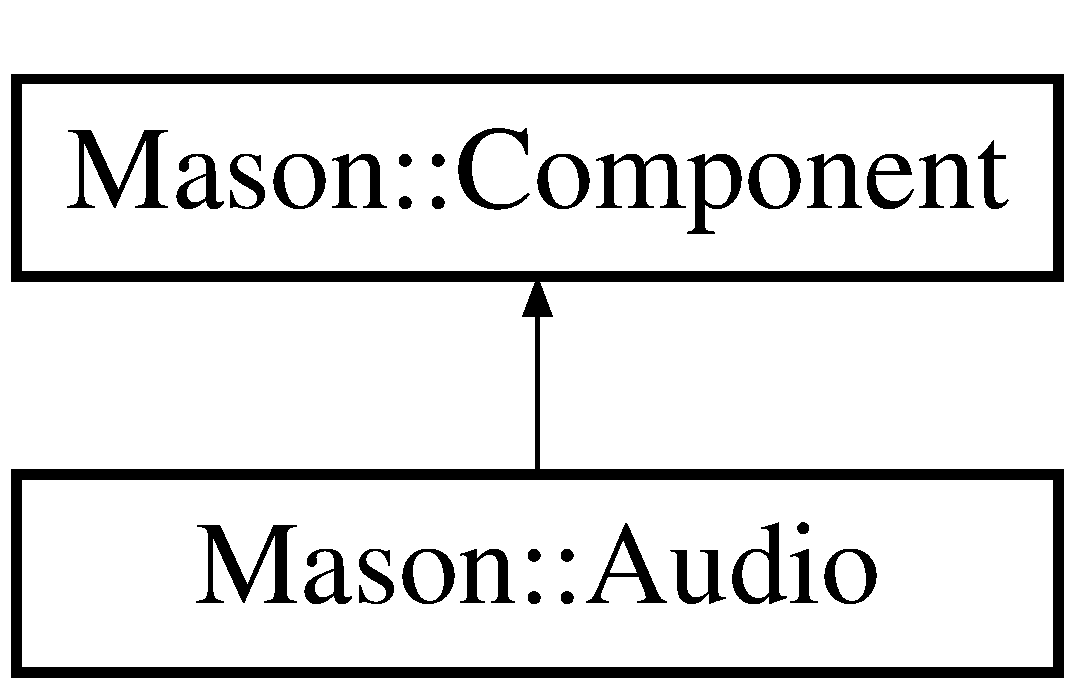
\includegraphics[height=2.000000cm]{class_mason_1_1_audio}
\end{center}
\end{figure}
\subsection*{Public Member Functions}
\begin{DoxyCompactItemize}
\item 
void \hyperlink{class_mason_1_1_audio_a5d4f318f5bee0b59d1a4289495b01b4c}{init} (std\+::string file, \hyperlink{namespace_mason_a158d651086d1ba1aacc4c37125b27657}{Sound\+Type} \hyperlink{class_mason_1_1_audio_a100d9da58685f865bf03dcf44a55fb63}{type}, \hyperlink{class_mason_1_1_audio_manager}{Audio\+Manager} $\ast$manager, int loops=0)
\begin{DoxyCompactList}\small\item\em Initializes the \hyperlink{class_mason_1_1_audio}{Audio} component. Calls the \hyperlink{class_mason_1_1_audio_manager}{Audio\+Manager} to load its \hyperlink{class_mason_1_1_audio}{Audio} Source. \end{DoxyCompactList}\item 
void \hyperlink{class_mason_1_1_audio_a2916f9015031bee9abb98adf0d83e7ee}{play} ()
\begin{DoxyCompactList}\small\item\em Plays the audio by querying the \hyperlink{class_mason_1_1_audio_manager}{Audio\+Manager}. \end{DoxyCompactList}\end{DoxyCompactItemize}
\subsection*{Public Attributes}
\begin{DoxyCompactItemize}
\item 
\hyperlink{namespace_mason_a158d651086d1ba1aacc4c37125b27657}{Sound\+Type} \hyperlink{class_mason_1_1_audio_a100d9da58685f865bf03dcf44a55fb63}{type}
\begin{DoxyCompactList}\small\item\em Holds the Sound\+Type enum. Either Sound\+Type\+::\+E\+F\+F\+E\+CT or Sound\+Type\+::\+Music. \end{DoxyCompactList}\item 
std\+::string \hyperlink{class_mason_1_1_audio_a762cc6174ce20a011fe1e3a36e649204}{path}
\begin{DoxyCompactList}\small\item\em Holds the path to the .wav audio file. \end{DoxyCompactList}\end{DoxyCompactItemize}
\subsection*{Protected Member Functions}
\begin{DoxyCompactItemize}
\item 
\hyperlink{class_mason_1_1_audio_aa65245dcba1c0a373b7130e7e36306c2}{Audio} (std\+::shared\+\_\+ptr$<$ \hyperlink{class_mason_1_1_game_object}{Game\+Object} $>$ \hyperlink{class_mason_1_1_component_abaa67b569d0a70e26a4606f4a099a925}{game\+Object})
\begin{DoxyCompactList}\small\item\em Constructor. \end{DoxyCompactList}\end{DoxyCompactItemize}
\subsection*{Friends}
\begin{DoxyCompactItemize}
\item 
class \hyperlink{class_mason_1_1_audio_a00df87c957d8f7ee0fc51f07a0542f4a}{Game\+Object}
\end{DoxyCompactItemize}
\subsection*{Additional Inherited Members}


\subsection{Detailed Description}
Extends the \hyperlink{class_mason_1_1_component}{Component} class and holds information about a .wav sound file. 

\subsection{Constructor \& Destructor Documentation}
\hypertarget{class_mason_1_1_audio_aa65245dcba1c0a373b7130e7e36306c2}{}\label{class_mason_1_1_audio_aa65245dcba1c0a373b7130e7e36306c2} 
\index{Mason\+::\+Audio@{Mason\+::\+Audio}!Audio@{Audio}}
\index{Audio@{Audio}!Mason\+::\+Audio@{Mason\+::\+Audio}}
\subsubsection{\texorpdfstring{Audio()}{Audio()}}
{\footnotesize\ttfamily Audio\+::\+Audio (\begin{DoxyParamCaption}\item[{std\+::shared\+\_\+ptr$<$ \hyperlink{class_mason_1_1_game_object}{Game\+Object} $>$}]{game\+Object }\end{DoxyParamCaption})\hspace{0.3cm}{\ttfamily [protected]}}



Constructor. 



\subsection{Member Function Documentation}
\hypertarget{class_mason_1_1_audio_a5d4f318f5bee0b59d1a4289495b01b4c}{}\label{class_mason_1_1_audio_a5d4f318f5bee0b59d1a4289495b01b4c} 
\index{Mason\+::\+Audio@{Mason\+::\+Audio}!init@{init}}
\index{init@{init}!Mason\+::\+Audio@{Mason\+::\+Audio}}
\subsubsection{\texorpdfstring{init()}{init()}}
{\footnotesize\ttfamily void Audio\+::init (\begin{DoxyParamCaption}\item[{std\+::string}]{file,  }\item[{\hyperlink{namespace_mason_a158d651086d1ba1aacc4c37125b27657}{Sound\+Type}}]{type,  }\item[{\hyperlink{class_mason_1_1_audio_manager}{Audio\+Manager} $\ast$}]{manager,  }\item[{int}]{loops = {\ttfamily 0} }\end{DoxyParamCaption})}



Initializes the \hyperlink{class_mason_1_1_audio}{Audio} component. Calls the \hyperlink{class_mason_1_1_audio_manager}{Audio\+Manager} to load its \hyperlink{class_mason_1_1_audio}{Audio} Source. 


\begin{DoxyParams}{Parameters}
{\em file} & path to a .wav sound file. Must be a .wav file. \\
\hline
{\em type} & either Sound\+Type\+::\+E\+F\+F\+E\+CT for Sound Effect or Soundtype\+::\+M\+U\+S\+IC for music. \\
\hline
{\em manager} & pointer to the active \hyperlink{class_mason_1_1_audio_manager}{Audio\+Manager} \\
\hline
{\em loops} & currently unused. \\
\hline
\end{DoxyParams}
\hypertarget{class_mason_1_1_audio_a2916f9015031bee9abb98adf0d83e7ee}{}\label{class_mason_1_1_audio_a2916f9015031bee9abb98adf0d83e7ee} 
\index{Mason\+::\+Audio@{Mason\+::\+Audio}!play@{play}}
\index{play@{play}!Mason\+::\+Audio@{Mason\+::\+Audio}}
\subsubsection{\texorpdfstring{play()}{play()}}
{\footnotesize\ttfamily void Audio\+::play (\begin{DoxyParamCaption}{ }\end{DoxyParamCaption})}



Plays the audio by querying the \hyperlink{class_mason_1_1_audio_manager}{Audio\+Manager}. 



\subsection{Friends And Related Function Documentation}
\hypertarget{class_mason_1_1_audio_a00df87c957d8f7ee0fc51f07a0542f4a}{}\label{class_mason_1_1_audio_a00df87c957d8f7ee0fc51f07a0542f4a} 
\index{Mason\+::\+Audio@{Mason\+::\+Audio}!Game\+Object@{Game\+Object}}
\index{Game\+Object@{Game\+Object}!Mason\+::\+Audio@{Mason\+::\+Audio}}
\subsubsection{\texorpdfstring{Game\+Object}{GameObject}}
{\footnotesize\ttfamily friend class \hyperlink{class_mason_1_1_game_object}{Game\+Object}\hspace{0.3cm}{\ttfamily [friend]}}



\subsection{Member Data Documentation}
\hypertarget{class_mason_1_1_audio_a762cc6174ce20a011fe1e3a36e649204}{}\label{class_mason_1_1_audio_a762cc6174ce20a011fe1e3a36e649204} 
\index{Mason\+::\+Audio@{Mason\+::\+Audio}!path@{path}}
\index{path@{path}!Mason\+::\+Audio@{Mason\+::\+Audio}}
\subsubsection{\texorpdfstring{path}{path}}
{\footnotesize\ttfamily std\+::string Mason\+::\+Audio\+::path}



Holds the path to the .wav audio file. 

\hypertarget{class_mason_1_1_audio_a100d9da58685f865bf03dcf44a55fb63}{}\label{class_mason_1_1_audio_a100d9da58685f865bf03dcf44a55fb63} 
\index{Mason\+::\+Audio@{Mason\+::\+Audio}!type@{type}}
\index{type@{type}!Mason\+::\+Audio@{Mason\+::\+Audio}}
\subsubsection{\texorpdfstring{type}{type}}
{\footnotesize\ttfamily \hyperlink{namespace_mason_a158d651086d1ba1aacc4c37125b27657}{Sound\+Type} Mason\+::\+Audio\+::type}



Holds the Sound\+Type enum. Either Sound\+Type\+::\+E\+F\+F\+E\+CT or Sound\+Type\+::\+Music. 



The documentation for this class was generated from the following files\+:\begin{DoxyCompactItemize}
\item 
include/\+Mason/\hyperlink{_audio_8hpp}{Audio.\+hpp}\item 
src/\hyperlink{_audio_8cpp}{Audio.\+cpp}\end{DoxyCompactItemize}

\hypertarget{class_mason_1_1_audio_descriptor}{}\section{Mason\+:\+:Audio\+Descriptor Class Reference}
\label{class_mason_1_1_audio_descriptor}\index{Mason\+::\+Audio\+Descriptor@{Mason\+::\+Audio\+Descriptor}}


Describes an \hyperlink{class_mason_1_1_audio}{Audio} component ~\newline
  




{\ttfamily \#include $<$Scene\+Parser.\+hpp$>$}

\subsection*{Public Attributes}
\begin{DoxyCompactItemize}
\item 
std\+::string \hyperlink{class_mason_1_1_audio_descriptor_a48908da92ad467deffccb4d8340aea20}{path}
\item 
\hyperlink{namespace_mason_a158d651086d1ba1aacc4c37125b27657}{Sound\+Type} \hyperlink{class_mason_1_1_audio_descriptor_af0235fd20741197930246f28acb5113b}{type} =\hyperlink{namespace_mason_a158d651086d1ba1aacc4c37125b27657a3ee843ce73fc06de504eb1480c65c82f}{E\+F\+F\+E\+CT}
\item 
bool \hyperlink{class_mason_1_1_audio_descriptor_ab49d1cfecfbd13d161f1bad522bd3294}{found} = false
\end{DoxyCompactItemize}


\subsection{Detailed Description}
Describes an \hyperlink{class_mason_1_1_audio}{Audio} component ~\newline
 

\char`\"{}audio\char`\"{}\+: \{ ~\newline
 \char`\"{}path\char`\"{}\+: \char`\"{}data/sounds/1-\/octave/\+A5.\+wav\char`\"{}, // Mandatory ~\newline
 \char`\"{}type\char`\"{}\+: \char`\"{}soundeffect\char`\"{} // Optional. Options\+: \char`\"{}soundeffect\char`\"{} (default) $\vert$ \char`\"{}music\char`\"{} ~\newline
 \} 

\subsection{Member Data Documentation}
\hypertarget{class_mason_1_1_audio_descriptor_ab49d1cfecfbd13d161f1bad522bd3294}{}\label{class_mason_1_1_audio_descriptor_ab49d1cfecfbd13d161f1bad522bd3294} 
\index{Mason\+::\+Audio\+Descriptor@{Mason\+::\+Audio\+Descriptor}!found@{found}}
\index{found@{found}!Mason\+::\+Audio\+Descriptor@{Mason\+::\+Audio\+Descriptor}}
\subsubsection{\texorpdfstring{found}{found}}
{\footnotesize\ttfamily bool Mason\+::\+Audio\+Descriptor\+::found = false}

\hypertarget{class_mason_1_1_audio_descriptor_a48908da92ad467deffccb4d8340aea20}{}\label{class_mason_1_1_audio_descriptor_a48908da92ad467deffccb4d8340aea20} 
\index{Mason\+::\+Audio\+Descriptor@{Mason\+::\+Audio\+Descriptor}!path@{path}}
\index{path@{path}!Mason\+::\+Audio\+Descriptor@{Mason\+::\+Audio\+Descriptor}}
\subsubsection{\texorpdfstring{path}{path}}
{\footnotesize\ttfamily std\+::string Mason\+::\+Audio\+Descriptor\+::path}

\hypertarget{class_mason_1_1_audio_descriptor_af0235fd20741197930246f28acb5113b}{}\label{class_mason_1_1_audio_descriptor_af0235fd20741197930246f28acb5113b} 
\index{Mason\+::\+Audio\+Descriptor@{Mason\+::\+Audio\+Descriptor}!type@{type}}
\index{type@{type}!Mason\+::\+Audio\+Descriptor@{Mason\+::\+Audio\+Descriptor}}
\subsubsection{\texorpdfstring{type}{type}}
{\footnotesize\ttfamily \hyperlink{namespace_mason_a158d651086d1ba1aacc4c37125b27657}{Sound\+Type} Mason\+::\+Audio\+Descriptor\+::type =\hyperlink{namespace_mason_a158d651086d1ba1aacc4c37125b27657a3ee843ce73fc06de504eb1480c65c82f}{E\+F\+F\+E\+CT}}



The documentation for this class was generated from the following file\+:\begin{DoxyCompactItemize}
\item 
include/\+Mason/\hyperlink{_scene_parser_8hpp}{Scene\+Parser.\+hpp}\end{DoxyCompactItemize}

\hypertarget{class_mason_1_1_audio_manager}{}\section{Mason\+:\+:Audio\+Manager Class Reference}
\label{class_mason_1_1_audio_manager}\index{Mason\+::\+Audio\+Manager@{Mason\+::\+Audio\+Manager}}


{\ttfamily \#include $<$Audio\+Manager.\+hpp$>$}

\subsection*{Public Member Functions}
\begin{DoxyCompactItemize}
\item 
void \hyperlink{class_mason_1_1_audio_manager_a81eb2ff2bc2d1242e532c208b32d17ec}{step} ()
\item 
void \hyperlink{class_mason_1_1_audio_manager_aab6ee58a5f26c1397ca72af21247d46d}{Add\+Audio\+Source} (\hyperlink{class_mason_1_1_audio}{Audio} $\ast$audio\+Component)
\end{DoxyCompactItemize}
\subsection*{Static Public Member Functions}
\begin{DoxyCompactItemize}
\item 
static \hyperlink{class_mason_1_1_audio_manager}{Audio\+Manager} $\ast$ \hyperlink{class_mason_1_1_audio_manager_a77de22887544ce37ae13d7c4d5cf7a79}{get\+Instance} ()
\end{DoxyCompactItemize}


\subsection{Member Function Documentation}
\hypertarget{class_mason_1_1_audio_manager_aab6ee58a5f26c1397ca72af21247d46d}{}\label{class_mason_1_1_audio_manager_aab6ee58a5f26c1397ca72af21247d46d} 
\index{Mason\+::\+Audio\+Manager@{Mason\+::\+Audio\+Manager}!Add\+Audio\+Source@{Add\+Audio\+Source}}
\index{Add\+Audio\+Source@{Add\+Audio\+Source}!Mason\+::\+Audio\+Manager@{Mason\+::\+Audio\+Manager}}
\subsubsection{\texorpdfstring{Add\+Audio\+Source()}{AddAudioSource()}}
{\footnotesize\ttfamily void Audio\+Manager\+::\+Add\+Audio\+Source (\begin{DoxyParamCaption}\item[{\hyperlink{class_mason_1_1_audio}{Audio} $\ast$}]{audio\+Component }\end{DoxyParamCaption})}

\hypertarget{class_mason_1_1_audio_manager_a77de22887544ce37ae13d7c4d5cf7a79}{}\label{class_mason_1_1_audio_manager_a77de22887544ce37ae13d7c4d5cf7a79} 
\index{Mason\+::\+Audio\+Manager@{Mason\+::\+Audio\+Manager}!get\+Instance@{get\+Instance}}
\index{get\+Instance@{get\+Instance}!Mason\+::\+Audio\+Manager@{Mason\+::\+Audio\+Manager}}
\subsubsection{\texorpdfstring{get\+Instance()}{getInstance()}}
{\footnotesize\ttfamily \hyperlink{class_mason_1_1_audio_manager}{Audio\+Manager} $\ast$ Audio\+Manager\+::get\+Instance (\begin{DoxyParamCaption}{ }\end{DoxyParamCaption})\hspace{0.3cm}{\ttfamily [static]}}

\hypertarget{class_mason_1_1_audio_manager_a81eb2ff2bc2d1242e532c208b32d17ec}{}\label{class_mason_1_1_audio_manager_a81eb2ff2bc2d1242e532c208b32d17ec} 
\index{Mason\+::\+Audio\+Manager@{Mason\+::\+Audio\+Manager}!step@{step}}
\index{step@{step}!Mason\+::\+Audio\+Manager@{Mason\+::\+Audio\+Manager}}
\subsubsection{\texorpdfstring{step()}{step()}}
{\footnotesize\ttfamily void Audio\+Manager\+::step (\begin{DoxyParamCaption}{ }\end{DoxyParamCaption})}



The documentation for this class was generated from the following files\+:\begin{DoxyCompactItemize}
\item 
C\+:/\+Users/\+Carol/\+Documents/\+Git\+Hub/\+Team\+Does\+Not\+Matter/\+Engine/include/\+Mason/\hyperlink{_audio_manager_8hpp}{Audio\+Manager.\+hpp}\item 
C\+:/\+Users/\+Carol/\+Documents/\+Git\+Hub/\+Team\+Does\+Not\+Matter/\+Engine/src/\hyperlink{_audio_manager_8cpp}{Audio\+Manager.\+cpp}\end{DoxyCompactItemize}

\hypertarget{class_mason_1_1_box_collider2_d}{}\section{Mason\+:\+:Box\+Collider2D Class Reference}
\label{class_mason_1_1_box_collider2_d}\index{Mason\+::\+Box\+Collider2D@{Mason\+::\+Box\+Collider2D}}


{\ttfamily \#include $<$Box\+Collider2\+D.\+hpp$>$}

Inheritance diagram for Mason\+:\+:Box\+Collider2D\+:\begin{figure}[H]
\begin{center}
\leavevmode
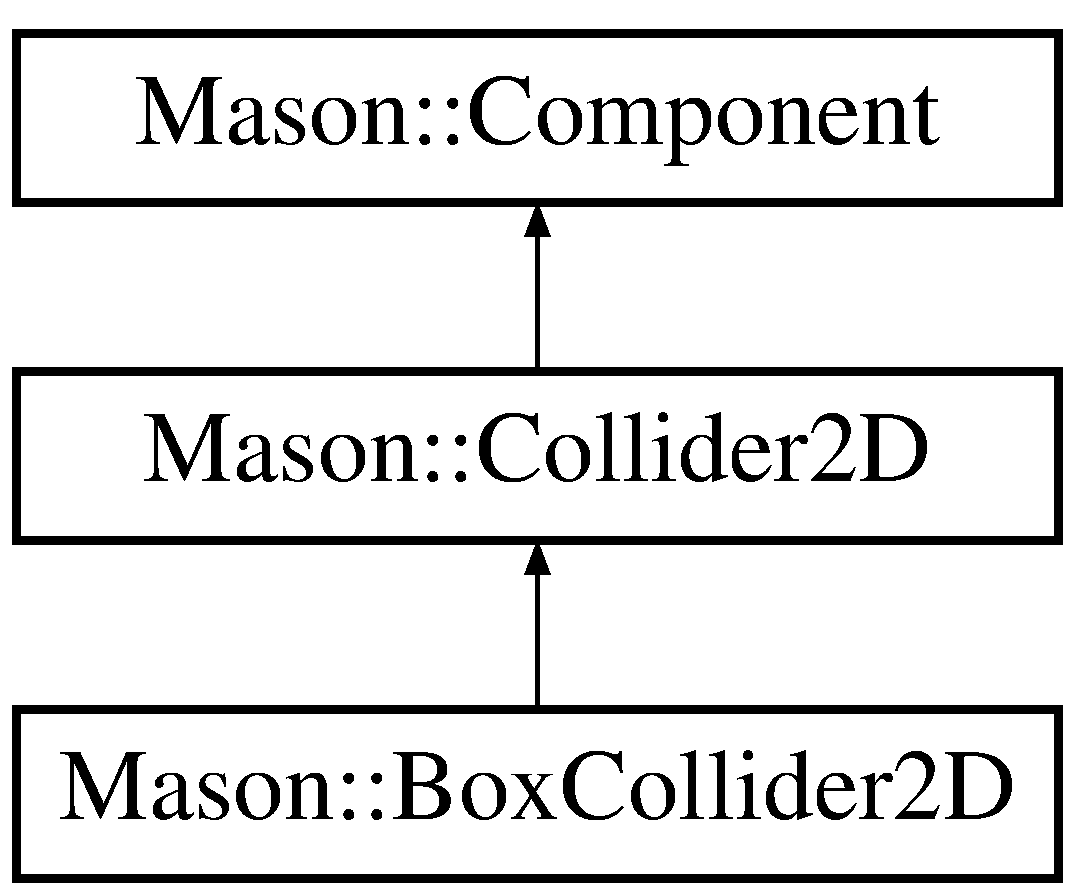
\includegraphics[height=3.000000cm]{class_mason_1_1_box_collider2_d}
\end{center}
\end{figure}
\subsection*{Public Member Functions}
\begin{DoxyCompactItemize}
\item 
void \hyperlink{class_mason_1_1_box_collider2_d_a4be834b1d746af44174f75e1c92cbbbc}{set\+Center} (float x, float y) const
\item 
void \hyperlink{class_mason_1_1_box_collider2_d_a57e51f07f4e6baf8533c05268f8ee0ed}{set\+Size} (float width, float height) const
\item 
\hyperlink{class_mason_1_1_box_collider2_d_a623201cca71e261e893b9ffa795eb4a7}{$\sim$\+Box\+Collider2D} ()
\end{DoxyCompactItemize}
\subsection*{Protected Member Functions}
\begin{DoxyCompactItemize}
\item 
\hyperlink{class_mason_1_1_box_collider2_d_a5b81f4bc97912c6f8375a427819d6d68}{Box\+Collider2D} (std\+::shared\+\_\+ptr$<$ \hyperlink{class_mason_1_1_game_object}{Game\+Object} $>$ \hyperlink{class_mason_1_1_component_abaa67b569d0a70e26a4606f4a099a925}{game\+Object})
\end{DoxyCompactItemize}
\subsection*{Friends}
\begin{DoxyCompactItemize}
\item 
class \hyperlink{class_mason_1_1_box_collider2_d_a00df87c957d8f7ee0fc51f07a0542f4a}{Game\+Object}
\end{DoxyCompactItemize}
\subsection*{Additional Inherited Members}


\subsection{Constructor \& Destructor Documentation}
\hypertarget{class_mason_1_1_box_collider2_d_a623201cca71e261e893b9ffa795eb4a7}{}\label{class_mason_1_1_box_collider2_d_a623201cca71e261e893b9ffa795eb4a7} 
\index{Mason\+::\+Box\+Collider2D@{Mason\+::\+Box\+Collider2D}!````~Box\+Collider2D@{$\sim$\+Box\+Collider2D}}
\index{````~Box\+Collider2D@{$\sim$\+Box\+Collider2D}!Mason\+::\+Box\+Collider2D@{Mason\+::\+Box\+Collider2D}}
\subsubsection{\texorpdfstring{$\sim$\+Box\+Collider2\+D()}{~BoxCollider2D()}}
{\footnotesize\ttfamily Box\+Collider2\+D\+::$\sim$\+Box\+Collider2D (\begin{DoxyParamCaption}{ }\end{DoxyParamCaption})}

\hypertarget{class_mason_1_1_box_collider2_d_a5b81f4bc97912c6f8375a427819d6d68}{}\label{class_mason_1_1_box_collider2_d_a5b81f4bc97912c6f8375a427819d6d68} 
\index{Mason\+::\+Box\+Collider2D@{Mason\+::\+Box\+Collider2D}!Box\+Collider2D@{Box\+Collider2D}}
\index{Box\+Collider2D@{Box\+Collider2D}!Mason\+::\+Box\+Collider2D@{Mason\+::\+Box\+Collider2D}}
\subsubsection{\texorpdfstring{Box\+Collider2\+D()}{BoxCollider2D()}}
{\footnotesize\ttfamily Box\+Collider2\+D\+::\+Box\+Collider2D (\begin{DoxyParamCaption}\item[{std\+::shared\+\_\+ptr$<$ \hyperlink{class_mason_1_1_game_object}{Game\+Object} $>$}]{game\+Object }\end{DoxyParamCaption})\hspace{0.3cm}{\ttfamily [protected]}}



\subsection{Member Function Documentation}
\hypertarget{class_mason_1_1_box_collider2_d_a4be834b1d746af44174f75e1c92cbbbc}{}\label{class_mason_1_1_box_collider2_d_a4be834b1d746af44174f75e1c92cbbbc} 
\index{Mason\+::\+Box\+Collider2D@{Mason\+::\+Box\+Collider2D}!set\+Center@{set\+Center}}
\index{set\+Center@{set\+Center}!Mason\+::\+Box\+Collider2D@{Mason\+::\+Box\+Collider2D}}
\subsubsection{\texorpdfstring{set\+Center()}{setCenter()}}
{\footnotesize\ttfamily void Box\+Collider2\+D\+::set\+Center (\begin{DoxyParamCaption}\item[{float}]{x,  }\item[{float}]{y }\end{DoxyParamCaption}) const}

\hypertarget{class_mason_1_1_box_collider2_d_a57e51f07f4e6baf8533c05268f8ee0ed}{}\label{class_mason_1_1_box_collider2_d_a57e51f07f4e6baf8533c05268f8ee0ed} 
\index{Mason\+::\+Box\+Collider2D@{Mason\+::\+Box\+Collider2D}!set\+Size@{set\+Size}}
\index{set\+Size@{set\+Size}!Mason\+::\+Box\+Collider2D@{Mason\+::\+Box\+Collider2D}}
\subsubsection{\texorpdfstring{set\+Size()}{setSize()}}
{\footnotesize\ttfamily void Box\+Collider2\+D\+::set\+Size (\begin{DoxyParamCaption}\item[{float}]{width,  }\item[{float}]{height }\end{DoxyParamCaption}) const}



\subsection{Friends And Related Function Documentation}
\hypertarget{class_mason_1_1_box_collider2_d_a00df87c957d8f7ee0fc51f07a0542f4a}{}\label{class_mason_1_1_box_collider2_d_a00df87c957d8f7ee0fc51f07a0542f4a} 
\index{Mason\+::\+Box\+Collider2D@{Mason\+::\+Box\+Collider2D}!Game\+Object@{Game\+Object}}
\index{Game\+Object@{Game\+Object}!Mason\+::\+Box\+Collider2D@{Mason\+::\+Box\+Collider2D}}
\subsubsection{\texorpdfstring{Game\+Object}{GameObject}}
{\footnotesize\ttfamily friend class \hyperlink{class_mason_1_1_game_object}{Game\+Object}\hspace{0.3cm}{\ttfamily [friend]}}



The documentation for this class was generated from the following files\+:\begin{DoxyCompactItemize}
\item 
include/\+Mason/\hyperlink{_box_collider2_d_8hpp}{Box\+Collider2\+D.\+hpp}\item 
src/\hyperlink{_box_collider2_d_8cpp}{Box\+Collider2\+D.\+cpp}\end{DoxyCompactItemize}

\hypertarget{class_mason_1_1_camera}{}\section{Mason\+:\+:Camera Class Reference}
\label{class_mason_1_1_camera}\index{Mason\+::\+Camera@{Mason\+::\+Camera}}


{\ttfamily \#include $<$Camera.\+hpp$>$}

Inheritance diagram for Mason\+:\+:Camera\+:\begin{figure}[H]
\begin{center}
\leavevmode
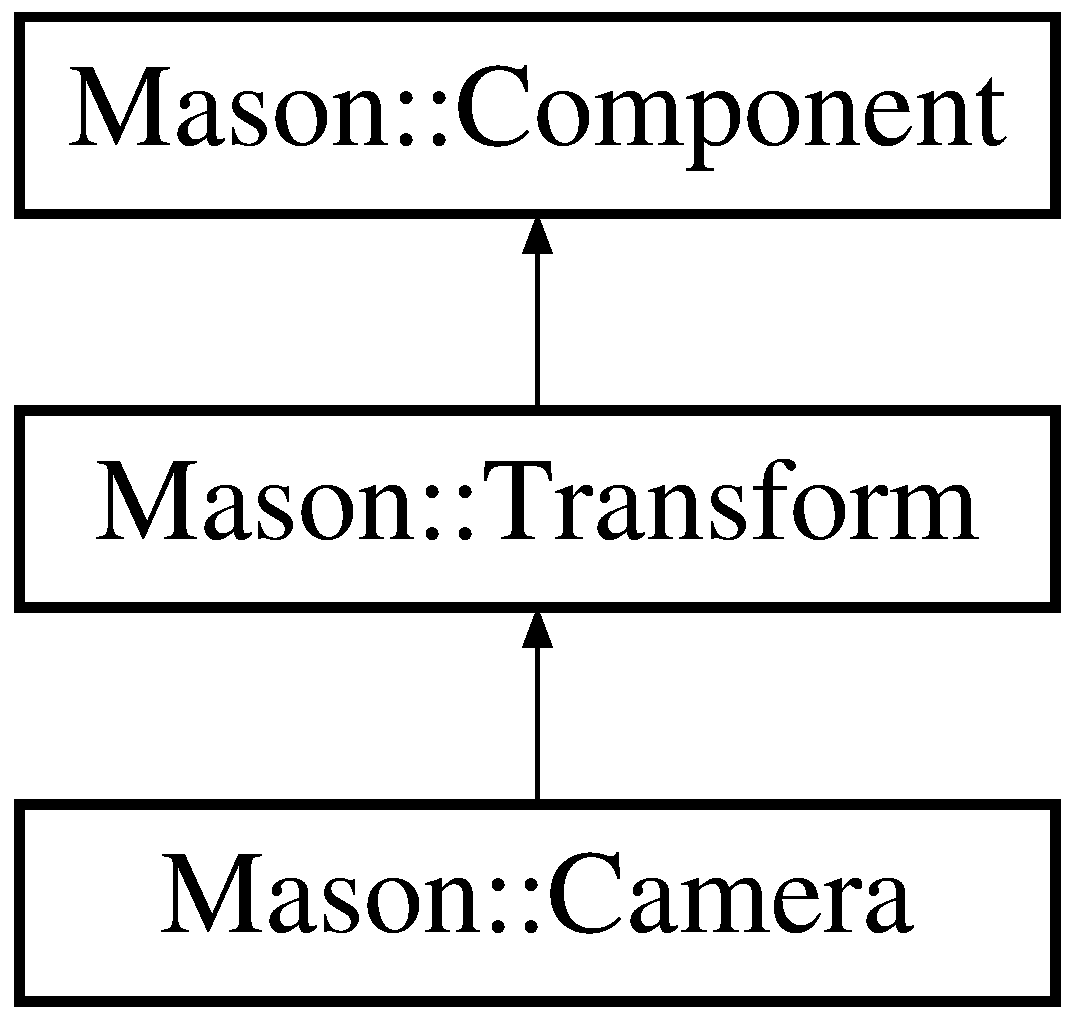
\includegraphics[height=3.000000cm]{class_mason_1_1_camera}
\end{center}
\end{figure}
\subsection*{Public Member Functions}
\begin{DoxyCompactItemize}
\item 
void \hyperlink{class_mason_1_1_camera_a732501ee31e862f557bbbc8ff58631a4}{set\+Scale} (glm\+::vec3 \hyperlink{class_mason_1_1_transform_a4618b31e34a6ec8a0ee638401fc56367}{scale}) override
\item 
void \hyperlink{class_mason_1_1_camera_a69f184af46d081b85209040bbe814cbb}{set\+Position} (glm\+::vec3 \hyperlink{class_mason_1_1_transform_ac9e11b4ec4433a38ac1100f12c955dcb}{position}) override
\item 
glm\+::vec3 \hyperlink{class_mason_1_1_camera_a405b26eaaae2ab7a460dfc319a9d16ea}{get\+Scale} () override
\item 
glm\+::vec3 \hyperlink{class_mason_1_1_camera_a71560b8b6216a542ae1958bd91a4361d}{get\+Position} () override
\item 
glm\+::vec2 \hyperlink{class_mason_1_1_camera_a0d2d26d8b7b80ab508ed4f4f537614b5}{get\+Viewport\+Min} () const
\item 
void \hyperlink{class_mason_1_1_camera_aa630259d7e0c0124dec5c9aaf33b7160}{set\+Viewport\+Min} (glm\+::vec2 viewport\+\_\+min)
\item 
glm\+::vec2 \hyperlink{class_mason_1_1_camera_abe43550148e85f5a32919a3c8b8ff115}{get\+Viewport\+Max} () const
\item 
void \hyperlink{class_mason_1_1_camera_a1f9a7896bb617d1402e3c4738324e1ea}{set\+Viewport\+Max} (glm\+::vec2 viewport\+\_\+max)
\item 
\hyperlink{class_mason_1_1_camera_ad1897942d0ccf91052386388a497349f}{$\sim$\+Camera} ()
\end{DoxyCompactItemize}
\subsection*{Protected Member Functions}
\begin{DoxyCompactItemize}
\item 
\hyperlink{class_mason_1_1_camera_aca4e1307d4601e7f0a711dfd94729143}{Camera} (\hyperlink{class_mason_1_1_game_object}{Game\+Object} $\ast$\hyperlink{class_mason_1_1_component_a30030370c35f5562cbbbb0927b0448c8}{game\+Object})
\item 
void \hyperlink{class_mason_1_1_camera_a27ff2d3ad004a49db2ae508ac6e9d3c2}{transformize} () override
\end{DoxyCompactItemize}
\subsection*{Protected Attributes}
\begin{DoxyCompactItemize}
\item 
glm\+::vec2 \hyperlink{class_mason_1_1_camera_a87d7d4111e63ecb41bac7ea33ef270e1}{viewport\+Min} = glm\+::vec2(0, 0)
\item 
glm\+::vec2 \hyperlink{class_mason_1_1_camera_a8c7510e4c83e123aebbe7bb36da80de9}{viewport\+Max} = glm\+::vec2(1, 1)
\item 
S\+R\+E\+::\+Camera $\ast$ \hyperlink{class_mason_1_1_camera_a74f870fa866086c21f28f0a1f59254cc}{cam}
\end{DoxyCompactItemize}
\subsection*{Friends}
\begin{DoxyCompactItemize}
\item 
class \hyperlink{class_mason_1_1_camera_a00df87c957d8f7ee0fc51f07a0542f4a}{Game\+Object}
\item 
class \hyperlink{class_mason_1_1_camera_a3e1914489e4bed4f9f23cdeab34a43dc}{Engine}
\end{DoxyCompactItemize}


\subsection{Constructor \& Destructor Documentation}
\hypertarget{class_mason_1_1_camera_ad1897942d0ccf91052386388a497349f}{}\label{class_mason_1_1_camera_ad1897942d0ccf91052386388a497349f} 
\index{Mason\+::\+Camera@{Mason\+::\+Camera}!````~Camera@{$\sim$\+Camera}}
\index{````~Camera@{$\sim$\+Camera}!Mason\+::\+Camera@{Mason\+::\+Camera}}
\subsubsection{\texorpdfstring{$\sim$\+Camera()}{~Camera()}}
{\footnotesize\ttfamily Camera\+::$\sim$\+Camera (\begin{DoxyParamCaption}{ }\end{DoxyParamCaption})}

\hypertarget{class_mason_1_1_camera_aca4e1307d4601e7f0a711dfd94729143}{}\label{class_mason_1_1_camera_aca4e1307d4601e7f0a711dfd94729143} 
\index{Mason\+::\+Camera@{Mason\+::\+Camera}!Camera@{Camera}}
\index{Camera@{Camera}!Mason\+::\+Camera@{Mason\+::\+Camera}}
\subsubsection{\texorpdfstring{Camera()}{Camera()}}
{\footnotesize\ttfamily Camera\+::\+Camera (\begin{DoxyParamCaption}\item[{\hyperlink{class_mason_1_1_game_object}{Game\+Object} $\ast$}]{game\+Object }\end{DoxyParamCaption})\hspace{0.3cm}{\ttfamily [protected]}}



\subsection{Member Function Documentation}
\hypertarget{class_mason_1_1_camera_a71560b8b6216a542ae1958bd91a4361d}{}\label{class_mason_1_1_camera_a71560b8b6216a542ae1958bd91a4361d} 
\index{Mason\+::\+Camera@{Mason\+::\+Camera}!get\+Position@{get\+Position}}
\index{get\+Position@{get\+Position}!Mason\+::\+Camera@{Mason\+::\+Camera}}
\subsubsection{\texorpdfstring{get\+Position()}{getPosition()}}
{\footnotesize\ttfamily glm\+::vec3 Camera\+::get\+Position (\begin{DoxyParamCaption}{ }\end{DoxyParamCaption})\hspace{0.3cm}{\ttfamily [override]}, {\ttfamily [virtual]}}



Reimplemented from \hyperlink{class_mason_1_1_transform_a0b21f641e72d7b55f3a630b986d0b106}{Mason\+::\+Transform}.

\hypertarget{class_mason_1_1_camera_a405b26eaaae2ab7a460dfc319a9d16ea}{}\label{class_mason_1_1_camera_a405b26eaaae2ab7a460dfc319a9d16ea} 
\index{Mason\+::\+Camera@{Mason\+::\+Camera}!get\+Scale@{get\+Scale}}
\index{get\+Scale@{get\+Scale}!Mason\+::\+Camera@{Mason\+::\+Camera}}
\subsubsection{\texorpdfstring{get\+Scale()}{getScale()}}
{\footnotesize\ttfamily glm\+::vec3 Camera\+::get\+Scale (\begin{DoxyParamCaption}{ }\end{DoxyParamCaption})\hspace{0.3cm}{\ttfamily [override]}, {\ttfamily [virtual]}}



Reimplemented from \hyperlink{class_mason_1_1_transform_a24107560725b250c4c2e10ab98a6ac04}{Mason\+::\+Transform}.

\hypertarget{class_mason_1_1_camera_abe43550148e85f5a32919a3c8b8ff115}{}\label{class_mason_1_1_camera_abe43550148e85f5a32919a3c8b8ff115} 
\index{Mason\+::\+Camera@{Mason\+::\+Camera}!get\+Viewport\+Max@{get\+Viewport\+Max}}
\index{get\+Viewport\+Max@{get\+Viewport\+Max}!Mason\+::\+Camera@{Mason\+::\+Camera}}
\subsubsection{\texorpdfstring{get\+Viewport\+Max()}{getViewportMax()}}
{\footnotesize\ttfamily glm\+::vec2 Camera\+::get\+Viewport\+Max (\begin{DoxyParamCaption}{ }\end{DoxyParamCaption}) const}

\hypertarget{class_mason_1_1_camera_a0d2d26d8b7b80ab508ed4f4f537614b5}{}\label{class_mason_1_1_camera_a0d2d26d8b7b80ab508ed4f4f537614b5} 
\index{Mason\+::\+Camera@{Mason\+::\+Camera}!get\+Viewport\+Min@{get\+Viewport\+Min}}
\index{get\+Viewport\+Min@{get\+Viewport\+Min}!Mason\+::\+Camera@{Mason\+::\+Camera}}
\subsubsection{\texorpdfstring{get\+Viewport\+Min()}{getViewportMin()}}
{\footnotesize\ttfamily glm\+::vec2 Camera\+::get\+Viewport\+Min (\begin{DoxyParamCaption}{ }\end{DoxyParamCaption}) const}

\hypertarget{class_mason_1_1_camera_a69f184af46d081b85209040bbe814cbb}{}\label{class_mason_1_1_camera_a69f184af46d081b85209040bbe814cbb} 
\index{Mason\+::\+Camera@{Mason\+::\+Camera}!set\+Position@{set\+Position}}
\index{set\+Position@{set\+Position}!Mason\+::\+Camera@{Mason\+::\+Camera}}
\subsubsection{\texorpdfstring{set\+Position()}{setPosition()}}
{\footnotesize\ttfamily void Camera\+::set\+Position (\begin{DoxyParamCaption}\item[{glm\+::vec3}]{position }\end{DoxyParamCaption})\hspace{0.3cm}{\ttfamily [override]}, {\ttfamily [virtual]}}



Reimplemented from \hyperlink{class_mason_1_1_transform_a740f389e20c0190c52bcb893aeaa0490}{Mason\+::\+Transform}.

\hypertarget{class_mason_1_1_camera_a732501ee31e862f557bbbc8ff58631a4}{}\label{class_mason_1_1_camera_a732501ee31e862f557bbbc8ff58631a4} 
\index{Mason\+::\+Camera@{Mason\+::\+Camera}!set\+Scale@{set\+Scale}}
\index{set\+Scale@{set\+Scale}!Mason\+::\+Camera@{Mason\+::\+Camera}}
\subsubsection{\texorpdfstring{set\+Scale()}{setScale()}}
{\footnotesize\ttfamily void Camera\+::set\+Scale (\begin{DoxyParamCaption}\item[{glm\+::vec3}]{scale }\end{DoxyParamCaption})\hspace{0.3cm}{\ttfamily [override]}, {\ttfamily [virtual]}}



Reimplemented from \hyperlink{class_mason_1_1_transform_a4a273ac58f45b6ee9cf2b37cf661daac}{Mason\+::\+Transform}.

\hypertarget{class_mason_1_1_camera_a1f9a7896bb617d1402e3c4738324e1ea}{}\label{class_mason_1_1_camera_a1f9a7896bb617d1402e3c4738324e1ea} 
\index{Mason\+::\+Camera@{Mason\+::\+Camera}!set\+Viewport\+Max@{set\+Viewport\+Max}}
\index{set\+Viewport\+Max@{set\+Viewport\+Max}!Mason\+::\+Camera@{Mason\+::\+Camera}}
\subsubsection{\texorpdfstring{set\+Viewport\+Max()}{setViewportMax()}}
{\footnotesize\ttfamily void Camera\+::set\+Viewport\+Max (\begin{DoxyParamCaption}\item[{glm\+::vec2}]{viewport\+\_\+max }\end{DoxyParamCaption})}

\hypertarget{class_mason_1_1_camera_aa630259d7e0c0124dec5c9aaf33b7160}{}\label{class_mason_1_1_camera_aa630259d7e0c0124dec5c9aaf33b7160} 
\index{Mason\+::\+Camera@{Mason\+::\+Camera}!set\+Viewport\+Min@{set\+Viewport\+Min}}
\index{set\+Viewport\+Min@{set\+Viewport\+Min}!Mason\+::\+Camera@{Mason\+::\+Camera}}
\subsubsection{\texorpdfstring{set\+Viewport\+Min()}{setViewportMin()}}
{\footnotesize\ttfamily void Camera\+::set\+Viewport\+Min (\begin{DoxyParamCaption}\item[{glm\+::vec2}]{viewport\+\_\+min }\end{DoxyParamCaption})}

\hypertarget{class_mason_1_1_camera_a27ff2d3ad004a49db2ae508ac6e9d3c2}{}\label{class_mason_1_1_camera_a27ff2d3ad004a49db2ae508ac6e9d3c2} 
\index{Mason\+::\+Camera@{Mason\+::\+Camera}!transformize@{transformize}}
\index{transformize@{transformize}!Mason\+::\+Camera@{Mason\+::\+Camera}}
\subsubsection{\texorpdfstring{transformize()}{transformize()}}
{\footnotesize\ttfamily void Camera\+::transformize (\begin{DoxyParamCaption}{ }\end{DoxyParamCaption})\hspace{0.3cm}{\ttfamily [override]}, {\ttfamily [protected]}, {\ttfamily [virtual]}}



Reimplemented from \hyperlink{class_mason_1_1_transform_a4dd61568d49044377f3312397ffdafd1}{Mason\+::\+Transform}.



\subsection{Friends And Related Function Documentation}
\hypertarget{class_mason_1_1_camera_a3e1914489e4bed4f9f23cdeab34a43dc}{}\label{class_mason_1_1_camera_a3e1914489e4bed4f9f23cdeab34a43dc} 
\index{Mason\+::\+Camera@{Mason\+::\+Camera}!Engine@{Engine}}
\index{Engine@{Engine}!Mason\+::\+Camera@{Mason\+::\+Camera}}
\subsubsection{\texorpdfstring{Engine}{Engine}}
{\footnotesize\ttfamily friend class \hyperlink{class_mason_1_1_engine}{Engine}\hspace{0.3cm}{\ttfamily [friend]}}

\hypertarget{class_mason_1_1_camera_a00df87c957d8f7ee0fc51f07a0542f4a}{}\label{class_mason_1_1_camera_a00df87c957d8f7ee0fc51f07a0542f4a} 
\index{Mason\+::\+Camera@{Mason\+::\+Camera}!Game\+Object@{Game\+Object}}
\index{Game\+Object@{Game\+Object}!Mason\+::\+Camera@{Mason\+::\+Camera}}
\subsubsection{\texorpdfstring{Game\+Object}{GameObject}}
{\footnotesize\ttfamily friend class \hyperlink{class_mason_1_1_game_object}{Game\+Object}\hspace{0.3cm}{\ttfamily [friend]}}



\subsection{Member Data Documentation}
\hypertarget{class_mason_1_1_camera_a74f870fa866086c21f28f0a1f59254cc}{}\label{class_mason_1_1_camera_a74f870fa866086c21f28f0a1f59254cc} 
\index{Mason\+::\+Camera@{Mason\+::\+Camera}!cam@{cam}}
\index{cam@{cam}!Mason\+::\+Camera@{Mason\+::\+Camera}}
\subsubsection{\texorpdfstring{cam}{cam}}
{\footnotesize\ttfamily S\+R\+E\+::\+Camera$\ast$ Mason\+::\+Camera\+::cam\hspace{0.3cm}{\ttfamily [protected]}}

\hypertarget{class_mason_1_1_camera_a8c7510e4c83e123aebbe7bb36da80de9}{}\label{class_mason_1_1_camera_a8c7510e4c83e123aebbe7bb36da80de9} 
\index{Mason\+::\+Camera@{Mason\+::\+Camera}!viewport\+Max@{viewport\+Max}}
\index{viewport\+Max@{viewport\+Max}!Mason\+::\+Camera@{Mason\+::\+Camera}}
\subsubsection{\texorpdfstring{viewport\+Max}{viewportMax}}
{\footnotesize\ttfamily glm\+::vec2 Mason\+::\+Camera\+::viewport\+Max = glm\+::vec2(1, 1)\hspace{0.3cm}{\ttfamily [protected]}}

\hypertarget{class_mason_1_1_camera_a87d7d4111e63ecb41bac7ea33ef270e1}{}\label{class_mason_1_1_camera_a87d7d4111e63ecb41bac7ea33ef270e1} 
\index{Mason\+::\+Camera@{Mason\+::\+Camera}!viewport\+Min@{viewport\+Min}}
\index{viewport\+Min@{viewport\+Min}!Mason\+::\+Camera@{Mason\+::\+Camera}}
\subsubsection{\texorpdfstring{viewport\+Min}{viewportMin}}
{\footnotesize\ttfamily glm\+::vec2 Mason\+::\+Camera\+::viewport\+Min = glm\+::vec2(0, 0)\hspace{0.3cm}{\ttfamily [protected]}}



The documentation for this class was generated from the following files\+:\begin{DoxyCompactItemize}
\item 
C\+:/\+Users/\+Carol/\+Documents/\+Git\+Hub/\+Team\+Does\+Not\+Matter/\+Engine/include/\+Mason/\hyperlink{_camera_8hpp}{Camera.\+hpp}\item 
C\+:/\+Users/\+Carol/\+Documents/\+Git\+Hub/\+Team\+Does\+Not\+Matter/\+Engine/src/\hyperlink{_camera_8cpp}{Camera.\+cpp}\end{DoxyCompactItemize}

\hypertarget{class_mason_1_1_camera_descriptor}{}\section{Mason\+:\+:Camera\+Descriptor Class Reference}
\label{class_mason_1_1_camera_descriptor}\index{Mason\+::\+Camera\+Descriptor@{Mason\+::\+Camera\+Descriptor}}


{\ttfamily \#include $<$Scene\+Parser.\+hpp$>$}

\subsection*{Public Attributes}
\begin{DoxyCompactItemize}
\item 
bool \hyperlink{class_mason_1_1_camera_descriptor_a51ca9c821b638e93d9406d97a3d50041}{found} = false
\item 
glm\+::vec2 \hyperlink{class_mason_1_1_camera_descriptor_a2d135d0102e435f15cf6a9dde7d64b25}{viewport\+Min} = glm\+::vec2(0, 0)
\item 
glm\+::vec2 \hyperlink{class_mason_1_1_camera_descriptor_ac0a5eb6054280925fbda6a20bb56932d}{viewport\+Max} = glm\+::vec2(1, 1)
\end{DoxyCompactItemize}


\subsection{Member Data Documentation}
\hypertarget{class_mason_1_1_camera_descriptor_a51ca9c821b638e93d9406d97a3d50041}{}\label{class_mason_1_1_camera_descriptor_a51ca9c821b638e93d9406d97a3d50041} 
\index{Mason\+::\+Camera\+Descriptor@{Mason\+::\+Camera\+Descriptor}!found@{found}}
\index{found@{found}!Mason\+::\+Camera\+Descriptor@{Mason\+::\+Camera\+Descriptor}}
\subsubsection{\texorpdfstring{found}{found}}
{\footnotesize\ttfamily bool Mason\+::\+Camera\+Descriptor\+::found = false}

\hypertarget{class_mason_1_1_camera_descriptor_ac0a5eb6054280925fbda6a20bb56932d}{}\label{class_mason_1_1_camera_descriptor_ac0a5eb6054280925fbda6a20bb56932d} 
\index{Mason\+::\+Camera\+Descriptor@{Mason\+::\+Camera\+Descriptor}!viewport\+Max@{viewport\+Max}}
\index{viewport\+Max@{viewport\+Max}!Mason\+::\+Camera\+Descriptor@{Mason\+::\+Camera\+Descriptor}}
\subsubsection{\texorpdfstring{viewport\+Max}{viewportMax}}
{\footnotesize\ttfamily glm\+::vec2 Mason\+::\+Camera\+Descriptor\+::viewport\+Max = glm\+::vec2(1, 1)}

\hypertarget{class_mason_1_1_camera_descriptor_a2d135d0102e435f15cf6a9dde7d64b25}{}\label{class_mason_1_1_camera_descriptor_a2d135d0102e435f15cf6a9dde7d64b25} 
\index{Mason\+::\+Camera\+Descriptor@{Mason\+::\+Camera\+Descriptor}!viewport\+Min@{viewport\+Min}}
\index{viewport\+Min@{viewport\+Min}!Mason\+::\+Camera\+Descriptor@{Mason\+::\+Camera\+Descriptor}}
\subsubsection{\texorpdfstring{viewport\+Min}{viewportMin}}
{\footnotesize\ttfamily glm\+::vec2 Mason\+::\+Camera\+Descriptor\+::viewport\+Min = glm\+::vec2(0, 0)}



The documentation for this class was generated from the following file\+:\begin{DoxyCompactItemize}
\item 
C\+:/\+Users/\+Carol/\+Documents/\+Git\+Hub/\+Team\+Does\+Not\+Matter/\+Engine/include/\+Mason/\hyperlink{_scene_parser_8hpp}{Scene\+Parser.\+hpp}\end{DoxyCompactItemize}

\hypertarget{class_mason_1_1_circle_collider2_d}{}\section{Mason\+:\+:Circle\+Collider2D Class Reference}
\label{class_mason_1_1_circle_collider2_d}\index{Mason\+::\+Circle\+Collider2D@{Mason\+::\+Circle\+Collider2D}}


{\ttfamily \#include $<$Circle\+Collider2\+D.\+h$>$}



Inheritance diagram for Mason\+:\+:Circle\+Collider2D\+:
% FIG 0


Collaboration diagram for Mason\+:\+:Circle\+Collider2D\+:
% FIG 1
\subsection*{Public Member Functions}
\begin{DoxyCompactItemize}
\item 
void \hyperlink{class_mason_1_1_circle_collider2_d_aa0e943bbb6fb5b9f33110959a845ed76}{set\+Center} (float x, float y)
\item 
void \hyperlink{class_mason_1_1_circle_collider2_d_aa91dcf071566c9862cf1ac385ad9f4a9}{set\+Size} (float rad)
\item 
b2\+Vec2 \hyperlink{class_mason_1_1_circle_collider2_d_a4aa06f3ff8f00445a78f6b6a8b479ad0}{Get\+Scale} () override
\end{DoxyCompactItemize}
\subsection*{Protected Member Functions}
\begin{DoxyCompactItemize}
\item 
\hyperlink{class_mason_1_1_circle_collider2_d_ac713c4259ab552c74b291d0e17f0e98a}{Circle\+Collider2D} (\hyperlink{class_mason_1_1_game_object}{Game\+Object} $\ast$\hyperlink{class_mason_1_1_component_a30030370c35f5562cbbbb0927b0448c8}{game\+Object})
\end{DoxyCompactItemize}
\subsection*{Friends}
\begin{DoxyCompactItemize}
\item 
class \hyperlink{class_mason_1_1_circle_collider2_d_a00df87c957d8f7ee0fc51f07a0542f4a}{Game\+Object}
\end{DoxyCompactItemize}
\subsection*{Additional Inherited Members}


\subsection{Constructor \& Destructor Documentation}
\hypertarget{class_mason_1_1_circle_collider2_d_ac713c4259ab552c74b291d0e17f0e98a}{}\label{class_mason_1_1_circle_collider2_d_ac713c4259ab552c74b291d0e17f0e98a} 
\index{Mason\+::\+Circle\+Collider2D@{Mason\+::\+Circle\+Collider2D}!Circle\+Collider2D@{Circle\+Collider2D}}
\index{Circle\+Collider2D@{Circle\+Collider2D}!Mason\+::\+Circle\+Collider2D@{Mason\+::\+Circle\+Collider2D}}
\subsubsection{\texorpdfstring{Circle\+Collider2\+D()}{CircleCollider2D()}}
{\footnotesize\ttfamily Circle\+Collider2\+D\+::\+Circle\+Collider2D (\begin{DoxyParamCaption}\item[{\hyperlink{class_mason_1_1_game_object}{Game\+Object} $\ast$}]{game\+Object }\end{DoxyParamCaption})\hspace{0.3cm}{\ttfamily [protected]}}

Here is the call graph for this function\+:
% FIG 2


\subsection{Member Function Documentation}
\hypertarget{class_mason_1_1_circle_collider2_d_a4aa06f3ff8f00445a78f6b6a8b479ad0}{}\label{class_mason_1_1_circle_collider2_d_a4aa06f3ff8f00445a78f6b6a8b479ad0} 
\index{Mason\+::\+Circle\+Collider2D@{Mason\+::\+Circle\+Collider2D}!Get\+Scale@{Get\+Scale}}
\index{Get\+Scale@{Get\+Scale}!Mason\+::\+Circle\+Collider2D@{Mason\+::\+Circle\+Collider2D}}
\subsubsection{\texorpdfstring{Get\+Scale()}{GetScale()}}
{\footnotesize\ttfamily b2\+Vec2 Circle\+Collider2\+D\+::\+Get\+Scale (\begin{DoxyParamCaption}{ }\end{DoxyParamCaption})\hspace{0.3cm}{\ttfamily [override]}, {\ttfamily [virtual]}}



Implements \hyperlink{class_mason_1_1_collider2_d_a3394739f1fea805691ac2753a9272156}{Mason\+::\+Collider2D}.

\hypertarget{class_mason_1_1_circle_collider2_d_aa0e943bbb6fb5b9f33110959a845ed76}{}\label{class_mason_1_1_circle_collider2_d_aa0e943bbb6fb5b9f33110959a845ed76} 
\index{Mason\+::\+Circle\+Collider2D@{Mason\+::\+Circle\+Collider2D}!set\+Center@{set\+Center}}
\index{set\+Center@{set\+Center}!Mason\+::\+Circle\+Collider2D@{Mason\+::\+Circle\+Collider2D}}
\subsubsection{\texorpdfstring{set\+Center()}{setCenter()}}
{\footnotesize\ttfamily void Circle\+Collider2\+D\+::set\+Center (\begin{DoxyParamCaption}\item[{float}]{x,  }\item[{float}]{y }\end{DoxyParamCaption})}

\hypertarget{class_mason_1_1_circle_collider2_d_aa91dcf071566c9862cf1ac385ad9f4a9}{}\label{class_mason_1_1_circle_collider2_d_aa91dcf071566c9862cf1ac385ad9f4a9} 
\index{Mason\+::\+Circle\+Collider2D@{Mason\+::\+Circle\+Collider2D}!set\+Size@{set\+Size}}
\index{set\+Size@{set\+Size}!Mason\+::\+Circle\+Collider2D@{Mason\+::\+Circle\+Collider2D}}
\subsubsection{\texorpdfstring{set\+Size()}{setSize()}}
{\footnotesize\ttfamily void Circle\+Collider2\+D\+::set\+Size (\begin{DoxyParamCaption}\item[{float}]{rad }\end{DoxyParamCaption})}



\subsection{Friends And Related Function Documentation}
\hypertarget{class_mason_1_1_circle_collider2_d_a00df87c957d8f7ee0fc51f07a0542f4a}{}\label{class_mason_1_1_circle_collider2_d_a00df87c957d8f7ee0fc51f07a0542f4a} 
\index{Mason\+::\+Circle\+Collider2D@{Mason\+::\+Circle\+Collider2D}!Game\+Object@{Game\+Object}}
\index{Game\+Object@{Game\+Object}!Mason\+::\+Circle\+Collider2D@{Mason\+::\+Circle\+Collider2D}}
\subsubsection{\texorpdfstring{Game\+Object}{GameObject}}
{\footnotesize\ttfamily friend class \hyperlink{class_mason_1_1_game_object}{Game\+Object}\hspace{0.3cm}{\ttfamily [friend]}}



The documentation for this class was generated from the following files\+:\begin{DoxyCompactItemize}
\item 
include/\+Mason/\hyperlink{_circle_collider2_d_8h}{Circle\+Collider2\+D.\+h}\item 
src/\hyperlink{_circle_collider2_d_8cpp}{Circle\+Collider2\+D.\+cpp}\end{DoxyCompactItemize}

\hypertarget{class_mason_1_1_collider2_d}{}\section{Mason\+:\+:Collider2D Class Reference}
\label{class_mason_1_1_collider2_d}\index{Mason\+::\+Collider2D@{Mason\+::\+Collider2D}}


{\ttfamily \#include $<$Collider2\+D.\+hpp$>$}

Inheritance diagram for Mason\+:\+:Collider2D\+:\begin{figure}[H]
\begin{center}
\leavevmode
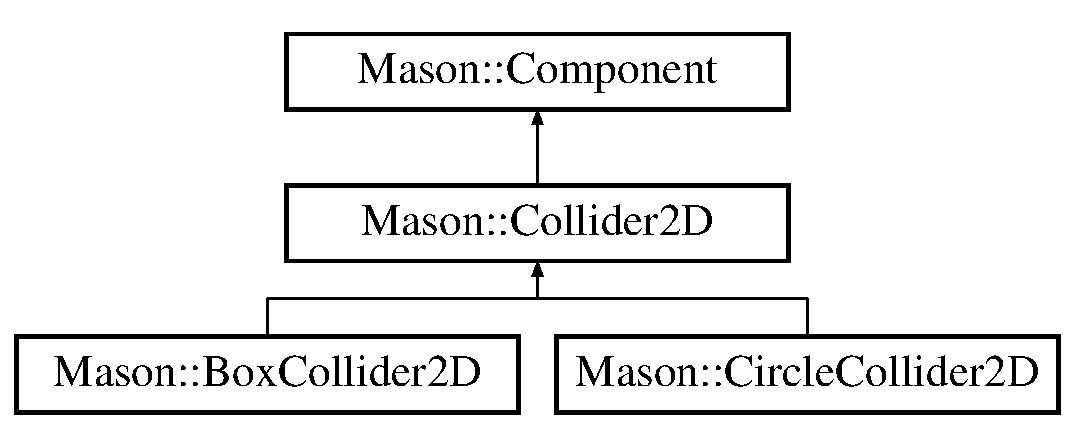
\includegraphics[height=3.000000cm]{class_mason_1_1_collider2_d}
\end{center}
\end{figure}
\subsection*{Public Member Functions}
\begin{DoxyCompactItemize}
\item 
virtual b2\+Vec2 \hyperlink{class_mason_1_1_collider2_d_a3394739f1fea805691ac2753a9272156}{Get\+Scale} ()=0
\end{DoxyCompactItemize}
\subsection*{Public Attributes}
\begin{DoxyCompactItemize}
\item 
b2\+Shape $\ast$ \hyperlink{class_mason_1_1_collider2_d_a82de033fe10f7da3fd079c7ff54eaf94}{shape}
\item 
float \hyperlink{class_mason_1_1_collider2_d_ad3b9178c829dbe0a8a25a75d643f8744}{density}
\item 
float \hyperlink{class_mason_1_1_collider2_d_ab08954cffa1ac7539e26c4e2da535481}{friction}
\end{DoxyCompactItemize}
\subsection*{Protected Member Functions}
\begin{DoxyCompactItemize}
\item 
\hyperlink{class_mason_1_1_collider2_d_a7ac26a9d09d5380b49027e9ae50fdacc}{Collider2D} (\hyperlink{class_mason_1_1_game_object}{Game\+Object} $\ast$\hyperlink{class_mason_1_1_component_a30030370c35f5562cbbbb0927b0448c8}{game\+Object})
\end{DoxyCompactItemize}
\subsection*{Friends}
\begin{DoxyCompactItemize}
\item 
class \hyperlink{class_mason_1_1_collider2_d_a00df87c957d8f7ee0fc51f07a0542f4a}{Game\+Object}
\end{DoxyCompactItemize}
\subsection*{Additional Inherited Members}


\subsection{Constructor \& Destructor Documentation}
\hypertarget{class_mason_1_1_collider2_d_a7ac26a9d09d5380b49027e9ae50fdacc}{}\label{class_mason_1_1_collider2_d_a7ac26a9d09d5380b49027e9ae50fdacc} 
\index{Mason\+::\+Collider2D@{Mason\+::\+Collider2D}!Collider2D@{Collider2D}}
\index{Collider2D@{Collider2D}!Mason\+::\+Collider2D@{Mason\+::\+Collider2D}}
\subsubsection{\texorpdfstring{Collider2\+D()}{Collider2D()}}
{\footnotesize\ttfamily Mason\+::\+Collider2\+D\+::\+Collider2D (\begin{DoxyParamCaption}\item[{\hyperlink{class_mason_1_1_game_object}{Game\+Object} $\ast$}]{game\+Object }\end{DoxyParamCaption})\hspace{0.3cm}{\ttfamily [inline]}, {\ttfamily [protected]}}



\subsection{Member Function Documentation}
\hypertarget{class_mason_1_1_collider2_d_a3394739f1fea805691ac2753a9272156}{}\label{class_mason_1_1_collider2_d_a3394739f1fea805691ac2753a9272156} 
\index{Mason\+::\+Collider2D@{Mason\+::\+Collider2D}!Get\+Scale@{Get\+Scale}}
\index{Get\+Scale@{Get\+Scale}!Mason\+::\+Collider2D@{Mason\+::\+Collider2D}}
\subsubsection{\texorpdfstring{Get\+Scale()}{GetScale()}}
{\footnotesize\ttfamily virtual b2\+Vec2 Mason\+::\+Collider2\+D\+::\+Get\+Scale (\begin{DoxyParamCaption}{ }\end{DoxyParamCaption})\hspace{0.3cm}{\ttfamily [pure virtual]}}



Implemented in \hyperlink{class_mason_1_1_box_collider2_d_a396aa615690a67c855b5025e3a1b3bce}{Mason\+::\+Box\+Collider2D}, and \hyperlink{class_mason_1_1_circle_collider2_d_a4aa06f3ff8f00445a78f6b6a8b479ad0}{Mason\+::\+Circle\+Collider2D}.



\subsection{Friends And Related Function Documentation}
\hypertarget{class_mason_1_1_collider2_d_a00df87c957d8f7ee0fc51f07a0542f4a}{}\label{class_mason_1_1_collider2_d_a00df87c957d8f7ee0fc51f07a0542f4a} 
\index{Mason\+::\+Collider2D@{Mason\+::\+Collider2D}!Game\+Object@{Game\+Object}}
\index{Game\+Object@{Game\+Object}!Mason\+::\+Collider2D@{Mason\+::\+Collider2D}}
\subsubsection{\texorpdfstring{Game\+Object}{GameObject}}
{\footnotesize\ttfamily friend class \hyperlink{class_mason_1_1_game_object}{Game\+Object}\hspace{0.3cm}{\ttfamily [friend]}}



\subsection{Member Data Documentation}
\hypertarget{class_mason_1_1_collider2_d_ad3b9178c829dbe0a8a25a75d643f8744}{}\label{class_mason_1_1_collider2_d_ad3b9178c829dbe0a8a25a75d643f8744} 
\index{Mason\+::\+Collider2D@{Mason\+::\+Collider2D}!density@{density}}
\index{density@{density}!Mason\+::\+Collider2D@{Mason\+::\+Collider2D}}
\subsubsection{\texorpdfstring{density}{density}}
{\footnotesize\ttfamily float Mason\+::\+Collider2\+D\+::density}

\hypertarget{class_mason_1_1_collider2_d_ab08954cffa1ac7539e26c4e2da535481}{}\label{class_mason_1_1_collider2_d_ab08954cffa1ac7539e26c4e2da535481} 
\index{Mason\+::\+Collider2D@{Mason\+::\+Collider2D}!friction@{friction}}
\index{friction@{friction}!Mason\+::\+Collider2D@{Mason\+::\+Collider2D}}
\subsubsection{\texorpdfstring{friction}{friction}}
{\footnotesize\ttfamily float Mason\+::\+Collider2\+D\+::friction}

\hypertarget{class_mason_1_1_collider2_d_a82de033fe10f7da3fd079c7ff54eaf94}{}\label{class_mason_1_1_collider2_d_a82de033fe10f7da3fd079c7ff54eaf94} 
\index{Mason\+::\+Collider2D@{Mason\+::\+Collider2D}!shape@{shape}}
\index{shape@{shape}!Mason\+::\+Collider2D@{Mason\+::\+Collider2D}}
\subsubsection{\texorpdfstring{shape}{shape}}
{\footnotesize\ttfamily b2\+Shape$\ast$ Mason\+::\+Collider2\+D\+::shape}



The documentation for this class was generated from the following file\+:\begin{DoxyCompactItemize}
\item 
C\+:/\+Users/\+Carol/\+Documents/\+Git\+Hub/\+Team\+Does\+Not\+Matter/\+Engine/include/\+Mason/\hyperlink{_collider2_d_8hpp}{Collider2\+D.\+hpp}\end{DoxyCompactItemize}

\hypertarget{class_mason_1_1_collision_listener}{}\section{Mason\+:\+:Collision\+Listener Class Reference}
\label{class_mason_1_1_collision_listener}\index{Mason\+::\+Collision\+Listener@{Mason\+::\+Collision\+Listener}}


{\ttfamily \#include $<$Collision\+Listener.\+h$>$}

Inheritance diagram for Mason\+:\+:Collision\+Listener\+:\begin{figure}[H]
\begin{center}
\leavevmode
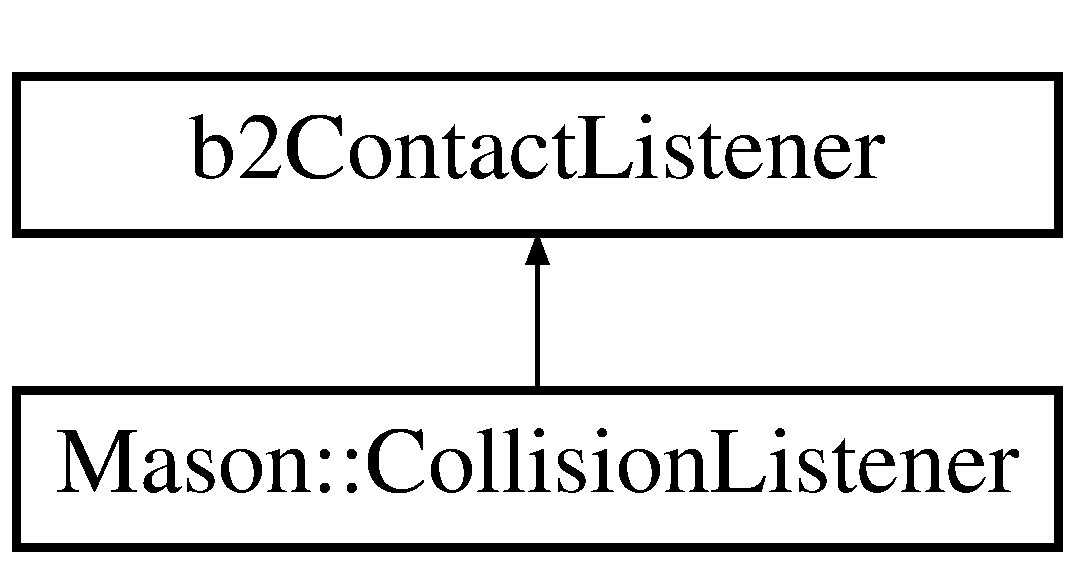
\includegraphics[height=2.000000cm]{class_mason_1_1_collision_listener}
\end{center}
\end{figure}
\subsection*{Public Member Functions}
\begin{DoxyCompactItemize}
\item 
void \hyperlink{class_mason_1_1_collision_listener_a10c4d83465cd2a9f6dd9d6e4dfba2834}{Process\+Events} ()
\item 
void \hyperlink{class_mason_1_1_collision_listener_ac65851c3fa2d3ee90d287fca613e20be}{Begin\+Contact} (b2\+Contact $\ast$contact) override
\item 
void \hyperlink{class_mason_1_1_collision_listener_a41a2b9775c5814c1446ceffdeb009640}{End\+Contact} (b2\+Contact $\ast$contact) override
\end{DoxyCompactItemize}


\subsection{Member Function Documentation}
\hypertarget{class_mason_1_1_collision_listener_ac65851c3fa2d3ee90d287fca613e20be}{}\label{class_mason_1_1_collision_listener_ac65851c3fa2d3ee90d287fca613e20be} 
\index{Mason\+::\+Collision\+Listener@{Mason\+::\+Collision\+Listener}!Begin\+Contact@{Begin\+Contact}}
\index{Begin\+Contact@{Begin\+Contact}!Mason\+::\+Collision\+Listener@{Mason\+::\+Collision\+Listener}}
\subsubsection{\texorpdfstring{Begin\+Contact()}{BeginContact()}}
{\footnotesize\ttfamily void Collision\+Listener\+::\+Begin\+Contact (\begin{DoxyParamCaption}\item[{b2\+Contact $\ast$}]{contact }\end{DoxyParamCaption})\hspace{0.3cm}{\ttfamily [override]}}

\hypertarget{class_mason_1_1_collision_listener_a41a2b9775c5814c1446ceffdeb009640}{}\label{class_mason_1_1_collision_listener_a41a2b9775c5814c1446ceffdeb009640} 
\index{Mason\+::\+Collision\+Listener@{Mason\+::\+Collision\+Listener}!End\+Contact@{End\+Contact}}
\index{End\+Contact@{End\+Contact}!Mason\+::\+Collision\+Listener@{Mason\+::\+Collision\+Listener}}
\subsubsection{\texorpdfstring{End\+Contact()}{EndContact()}}
{\footnotesize\ttfamily void Collision\+Listener\+::\+End\+Contact (\begin{DoxyParamCaption}\item[{b2\+Contact $\ast$}]{contact }\end{DoxyParamCaption})\hspace{0.3cm}{\ttfamily [override]}}

\hypertarget{class_mason_1_1_collision_listener_a10c4d83465cd2a9f6dd9d6e4dfba2834}{}\label{class_mason_1_1_collision_listener_a10c4d83465cd2a9f6dd9d6e4dfba2834} 
\index{Mason\+::\+Collision\+Listener@{Mason\+::\+Collision\+Listener}!Process\+Events@{Process\+Events}}
\index{Process\+Events@{Process\+Events}!Mason\+::\+Collision\+Listener@{Mason\+::\+Collision\+Listener}}
\subsubsection{\texorpdfstring{Process\+Events()}{ProcessEvents()}}
{\footnotesize\ttfamily void Collision\+Listener\+::\+Process\+Events (\begin{DoxyParamCaption}{ }\end{DoxyParamCaption})}



The documentation for this class was generated from the following files\+:\begin{DoxyCompactItemize}
\item 
include/\+Mason/\hyperlink{_collision_listener_8h}{Collision\+Listener.\+h}\item 
src/\hyperlink{_collision_listener_8cpp}{Collision\+Listener.\+cpp}\end{DoxyCompactItemize}

\hypertarget{class_mason_1_1_component}{}\section{Mason\+:\+:Component Class Reference}
\label{class_mason_1_1_component}\index{Mason\+::\+Component@{Mason\+::\+Component}}


{\ttfamily \#include $<$Component.\+hpp$>$}



Inheritance diagram for Mason\+:\+:Component\+:
% FIG 0


Collaboration diagram for Mason\+:\+:Component\+:
% FIG 1
\subsection*{Public Member Functions}
\begin{DoxyCompactItemize}
\item 
virtual \hyperlink{class_mason_1_1_component_ab8378fa275af98e568a7e91d33d867af}{$\sim$\+Component} ()
\item 
\hyperlink{class_mason_1_1_game_object}{Game\+Object} $\ast$ \hyperlink{class_mason_1_1_component_abed36db99f1ee0ba84a5fb8485e17428}{get\+Game\+Object} ()
\end{DoxyCompactItemize}
\subsection*{Protected Member Functions}
\begin{DoxyCompactItemize}
\item 
\hyperlink{class_mason_1_1_component_a98d3a7d72f88dc7e67c946c78afb8243}{Component} (\hyperlink{class_mason_1_1_game_object}{Game\+Object} $\ast$\hyperlink{class_mason_1_1_component_a30030370c35f5562cbbbb0927b0448c8}{game\+Object})
\end{DoxyCompactItemize}
\subsection*{Protected Attributes}
\begin{DoxyCompactItemize}
\item 
\hyperlink{class_mason_1_1_game_object}{Game\+Object} $\ast$ \hyperlink{class_mason_1_1_component_a30030370c35f5562cbbbb0927b0448c8}{game\+Object}
\end{DoxyCompactItemize}
\subsection*{Friends}
\begin{DoxyCompactItemize}
\item 
class \hyperlink{class_mason_1_1_component_a00df87c957d8f7ee0fc51f07a0542f4a}{Game\+Object}
\end{DoxyCompactItemize}


\subsection{Constructor \& Destructor Documentation}
\hypertarget{class_mason_1_1_component_ab8378fa275af98e568a7e91d33d867af}{}\label{class_mason_1_1_component_ab8378fa275af98e568a7e91d33d867af} 
\index{Mason\+::\+Component@{Mason\+::\+Component}!````~Component@{$\sim$\+Component}}
\index{````~Component@{$\sim$\+Component}!Mason\+::\+Component@{Mason\+::\+Component}}
\subsubsection{\texorpdfstring{$\sim$\+Component()}{~Component()}}
{\footnotesize\ttfamily Component\+::$\sim$\+Component (\begin{DoxyParamCaption}{ }\end{DoxyParamCaption})\hspace{0.3cm}{\ttfamily [virtual]}}

\hypertarget{class_mason_1_1_component_a98d3a7d72f88dc7e67c946c78afb8243}{}\label{class_mason_1_1_component_a98d3a7d72f88dc7e67c946c78afb8243} 
\index{Mason\+::\+Component@{Mason\+::\+Component}!Component@{Component}}
\index{Component@{Component}!Mason\+::\+Component@{Mason\+::\+Component}}
\subsubsection{\texorpdfstring{Component()}{Component()}}
{\footnotesize\ttfamily Component\+::\+Component (\begin{DoxyParamCaption}\item[{\hyperlink{class_mason_1_1_game_object}{Game\+Object} $\ast$}]{game\+Object }\end{DoxyParamCaption})\hspace{0.3cm}{\ttfamily [protected]}}



\subsection{Member Function Documentation}
\hypertarget{class_mason_1_1_component_abed36db99f1ee0ba84a5fb8485e17428}{}\label{class_mason_1_1_component_abed36db99f1ee0ba84a5fb8485e17428} 
\index{Mason\+::\+Component@{Mason\+::\+Component}!get\+Game\+Object@{get\+Game\+Object}}
\index{get\+Game\+Object@{get\+Game\+Object}!Mason\+::\+Component@{Mason\+::\+Component}}
\subsubsection{\texorpdfstring{get\+Game\+Object()}{getGameObject()}}
{\footnotesize\ttfamily \hyperlink{class_mason_1_1_game_object}{Game\+Object} $\ast$ Component\+::get\+Game\+Object (\begin{DoxyParamCaption}{ }\end{DoxyParamCaption})}



\subsection{Friends And Related Function Documentation}
\hypertarget{class_mason_1_1_component_a00df87c957d8f7ee0fc51f07a0542f4a}{}\label{class_mason_1_1_component_a00df87c957d8f7ee0fc51f07a0542f4a} 
\index{Mason\+::\+Component@{Mason\+::\+Component}!Game\+Object@{Game\+Object}}
\index{Game\+Object@{Game\+Object}!Mason\+::\+Component@{Mason\+::\+Component}}
\subsubsection{\texorpdfstring{Game\+Object}{GameObject}}
{\footnotesize\ttfamily friend class \hyperlink{class_mason_1_1_game_object}{Game\+Object}\hspace{0.3cm}{\ttfamily [friend]}}



\subsection{Member Data Documentation}
\hypertarget{class_mason_1_1_component_a30030370c35f5562cbbbb0927b0448c8}{}\label{class_mason_1_1_component_a30030370c35f5562cbbbb0927b0448c8} 
\index{Mason\+::\+Component@{Mason\+::\+Component}!game\+Object@{game\+Object}}
\index{game\+Object@{game\+Object}!Mason\+::\+Component@{Mason\+::\+Component}}
\subsubsection{\texorpdfstring{game\+Object}{gameObject}}
{\footnotesize\ttfamily \hyperlink{class_mason_1_1_game_object}{Game\+Object}$\ast$ Mason\+::\+Component\+::game\+Object\hspace{0.3cm}{\ttfamily [protected]}}



The documentation for this class was generated from the following files\+:\begin{DoxyCompactItemize}
\item 
include/\+Mason/\hyperlink{_component_8hpp}{Component.\+hpp}\item 
src/\hyperlink{_component_8cpp}{Component.\+cpp}\end{DoxyCompactItemize}

\hypertarget{class_mason_1_1_config}{}\section{Mason\+:\+:Config Class Reference}
\label{class_mason_1_1_config}\index{Mason\+::\+Config@{Mason\+::\+Config}}


{\ttfamily \#include $<$Config.\+hpp$>$}

\subsection*{Public Member Functions}
\begin{DoxyCompactItemize}
\item 
\hyperlink{class_mason_1_1_config_a543dce59b66475c5108088ee4ce1cdfc}{$\sim$\+Config} ()
\end{DoxyCompactItemize}
\subsection*{Static Public Member Functions}
\begin{DoxyCompactItemize}
\item 
static int $\ast$ \hyperlink{class_mason_1_1_config_af80adf2ed2290a3d714fb0407ee8fe55}{add\+Int} (std\+::string name, int value)
\item 
static float $\ast$ \hyperlink{class_mason_1_1_config_aa34f25a92ea33607425da418efabf47f}{add\+Float} (std\+::string name, float value)
\item 
static std\+::string $\ast$ \hyperlink{class_mason_1_1_config_a426f9e3f5de94a89dadfb7531d3b1d39}{add\+String} (std\+::string name, std\+::string value)
\item 
static int $\ast$ \hyperlink{class_mason_1_1_config_aafb3b1eb520c81f3002d4aa78e400ea0}{get\+Int} (std\+::string name)
\item 
static float $\ast$ \hyperlink{class_mason_1_1_config_a0e95110c092d4d3617a54a3ab3e4f70a}{get\+Float} (std\+::string name)
\item 
static std\+::string $\ast$ \hyperlink{class_mason_1_1_config_abc367cc6194d049807fab3ff684996e3}{get\+String} (std\+::string name)
\item 
static void \hyperlink{class_mason_1_1_config_a91bcb187ed95ec673137e413a4d77203}{init} ()
\end{DoxyCompactItemize}
\subsection*{Friends}
\begin{DoxyCompactItemize}
\item 
class \hyperlink{class_mason_1_1_config_a3e1914489e4bed4f9f23cdeab34a43dc}{Engine}
\end{DoxyCompactItemize}


\subsection{Constructor \& Destructor Documentation}
\hypertarget{class_mason_1_1_config_a543dce59b66475c5108088ee4ce1cdfc}{}\label{class_mason_1_1_config_a543dce59b66475c5108088ee4ce1cdfc} 
\index{Mason\+::\+Config@{Mason\+::\+Config}!````~Config@{$\sim$\+Config}}
\index{````~Config@{$\sim$\+Config}!Mason\+::\+Config@{Mason\+::\+Config}}
\subsubsection{\texorpdfstring{$\sim$\+Config()}{~Config()}}
{\footnotesize\ttfamily Config\+::$\sim$\+Config (\begin{DoxyParamCaption}{ }\end{DoxyParamCaption})}



\subsection{Member Function Documentation}
\hypertarget{class_mason_1_1_config_aa34f25a92ea33607425da418efabf47f}{}\label{class_mason_1_1_config_aa34f25a92ea33607425da418efabf47f} 
\index{Mason\+::\+Config@{Mason\+::\+Config}!add\+Float@{add\+Float}}
\index{add\+Float@{add\+Float}!Mason\+::\+Config@{Mason\+::\+Config}}
\subsubsection{\texorpdfstring{add\+Float()}{addFloat()}}
{\footnotesize\ttfamily float $\ast$ Config\+::add\+Float (\begin{DoxyParamCaption}\item[{std\+::string}]{name,  }\item[{float}]{value }\end{DoxyParamCaption})\hspace{0.3cm}{\ttfamily [static]}}

\hypertarget{class_mason_1_1_config_af80adf2ed2290a3d714fb0407ee8fe55}{}\label{class_mason_1_1_config_af80adf2ed2290a3d714fb0407ee8fe55} 
\index{Mason\+::\+Config@{Mason\+::\+Config}!add\+Int@{add\+Int}}
\index{add\+Int@{add\+Int}!Mason\+::\+Config@{Mason\+::\+Config}}
\subsubsection{\texorpdfstring{add\+Int()}{addInt()}}
{\footnotesize\ttfamily int $\ast$ Config\+::add\+Int (\begin{DoxyParamCaption}\item[{std\+::string}]{name,  }\item[{int}]{value }\end{DoxyParamCaption})\hspace{0.3cm}{\ttfamily [static]}}

\hypertarget{class_mason_1_1_config_a426f9e3f5de94a89dadfb7531d3b1d39}{}\label{class_mason_1_1_config_a426f9e3f5de94a89dadfb7531d3b1d39} 
\index{Mason\+::\+Config@{Mason\+::\+Config}!add\+String@{add\+String}}
\index{add\+String@{add\+String}!Mason\+::\+Config@{Mason\+::\+Config}}
\subsubsection{\texorpdfstring{add\+String()}{addString()}}
{\footnotesize\ttfamily std\+::string $\ast$ Config\+::add\+String (\begin{DoxyParamCaption}\item[{std\+::string}]{name,  }\item[{std\+::string}]{value }\end{DoxyParamCaption})\hspace{0.3cm}{\ttfamily [static]}}

\hypertarget{class_mason_1_1_config_a0e95110c092d4d3617a54a3ab3e4f70a}{}\label{class_mason_1_1_config_a0e95110c092d4d3617a54a3ab3e4f70a} 
\index{Mason\+::\+Config@{Mason\+::\+Config}!get\+Float@{get\+Float}}
\index{get\+Float@{get\+Float}!Mason\+::\+Config@{Mason\+::\+Config}}
\subsubsection{\texorpdfstring{get\+Float()}{getFloat()}}
{\footnotesize\ttfamily float $\ast$ Config\+::get\+Float (\begin{DoxyParamCaption}\item[{std\+::string}]{name }\end{DoxyParamCaption})\hspace{0.3cm}{\ttfamily [static]}}

\hypertarget{class_mason_1_1_config_aafb3b1eb520c81f3002d4aa78e400ea0}{}\label{class_mason_1_1_config_aafb3b1eb520c81f3002d4aa78e400ea0} 
\index{Mason\+::\+Config@{Mason\+::\+Config}!get\+Int@{get\+Int}}
\index{get\+Int@{get\+Int}!Mason\+::\+Config@{Mason\+::\+Config}}
\subsubsection{\texorpdfstring{get\+Int()}{getInt()}}
{\footnotesize\ttfamily int $\ast$ Config\+::get\+Int (\begin{DoxyParamCaption}\item[{std\+::string}]{name }\end{DoxyParamCaption})\hspace{0.3cm}{\ttfamily [static]}}

\hypertarget{class_mason_1_1_config_abc367cc6194d049807fab3ff684996e3}{}\label{class_mason_1_1_config_abc367cc6194d049807fab3ff684996e3} 
\index{Mason\+::\+Config@{Mason\+::\+Config}!get\+String@{get\+String}}
\index{get\+String@{get\+String}!Mason\+::\+Config@{Mason\+::\+Config}}
\subsubsection{\texorpdfstring{get\+String()}{getString()}}
{\footnotesize\ttfamily std\+::string $\ast$ Config\+::get\+String (\begin{DoxyParamCaption}\item[{std\+::string}]{name }\end{DoxyParamCaption})\hspace{0.3cm}{\ttfamily [static]}}

\hypertarget{class_mason_1_1_config_a91bcb187ed95ec673137e413a4d77203}{}\label{class_mason_1_1_config_a91bcb187ed95ec673137e413a4d77203} 
\index{Mason\+::\+Config@{Mason\+::\+Config}!init@{init}}
\index{init@{init}!Mason\+::\+Config@{Mason\+::\+Config}}
\subsubsection{\texorpdfstring{init()}{init()}}
{\footnotesize\ttfamily void Config\+::init (\begin{DoxyParamCaption}{ }\end{DoxyParamCaption})\hspace{0.3cm}{\ttfamily [static]}}



\subsection{Friends And Related Function Documentation}
\hypertarget{class_mason_1_1_config_a3e1914489e4bed4f9f23cdeab34a43dc}{}\label{class_mason_1_1_config_a3e1914489e4bed4f9f23cdeab34a43dc} 
\index{Mason\+::\+Config@{Mason\+::\+Config}!Engine@{Engine}}
\index{Engine@{Engine}!Mason\+::\+Config@{Mason\+::\+Config}}
\subsubsection{\texorpdfstring{Engine}{Engine}}
{\footnotesize\ttfamily friend class \hyperlink{class_mason_1_1_engine}{Engine}\hspace{0.3cm}{\ttfamily [friend]}}



The documentation for this class was generated from the following files\+:\begin{DoxyCompactItemize}
\item 
C\+:/\+Users/\+Carol/\+Documents/\+Git\+Hub/\+Team\+Does\+Not\+Matter/\+Engine/include/\+Mason/\hyperlink{_config_8hpp}{Config.\+hpp}\item 
C\+:/\+Users/\+Carol/\+Documents/\+Git\+Hub/\+Team\+Does\+Not\+Matter/\+Engine/src/\hyperlink{_config_8cpp}{Config.\+cpp}\end{DoxyCompactItemize}

\hypertarget{classpicojson_1_1default__parse__context}{}\section{picojson\+:\+:default\+\_\+parse\+\_\+context Class Reference}
\label{classpicojson_1_1default__parse__context}\index{picojson\+::default\+\_\+parse\+\_\+context@{picojson\+::default\+\_\+parse\+\_\+context}}


{\ttfamily \#include $<$picojson.\+h$>$}

\subsection*{Public Member Functions}
\begin{DoxyCompactItemize}
\item 
\hyperlink{classpicojson_1_1default__parse__context_ad326572abe85f9d05dc23be4cf76ff3c}{default\+\_\+parse\+\_\+context} (\hyperlink{classpicojson_1_1value}{value} $\ast$out)
\item 
bool \hyperlink{classpicojson_1_1default__parse__context_a2d852ba1f0b115c89378fcb5f10580b5}{set\+\_\+null} ()
\item 
bool \hyperlink{classpicojson_1_1default__parse__context_ae1935ef455fc2bed9195426cfee5713a}{set\+\_\+bool} (bool b)
\item 
bool \hyperlink{classpicojson_1_1default__parse__context_a9b2046a9cb6d66aad835b84ffda20b86}{set\+\_\+number} (double f)
\item 
{\footnotesize template$<$typename Iter $>$ }\\bool \hyperlink{classpicojson_1_1default__parse__context_a476c7d30a5cf382b48201ec64585c2f3}{parse\+\_\+string} (\hyperlink{classpicojson_1_1input}{input}$<$ Iter $>$ \&in)
\item 
bool \hyperlink{classpicojson_1_1default__parse__context_a5c355f843ceacde134997f5bbbda1d23}{parse\+\_\+array\+\_\+start} ()
\item 
{\footnotesize template$<$typename Iter $>$ }\\bool \hyperlink{classpicojson_1_1default__parse__context_a5f65224e655633b20c1f8c5967c153bb}{parse\+\_\+array\+\_\+item} (\hyperlink{classpicojson_1_1input}{input}$<$ Iter $>$ \&in, size\+\_\+t)
\item 
bool \hyperlink{classpicojson_1_1default__parse__context_aa6ac46d87d620377429438675ba9fab2}{parse\+\_\+array\+\_\+stop} (size\+\_\+t)
\item 
bool \hyperlink{classpicojson_1_1default__parse__context_a54eba00b93ce4cdaf8b2acac4ef3e046}{parse\+\_\+object\+\_\+start} ()
\item 
{\footnotesize template$<$typename Iter $>$ }\\bool \hyperlink{classpicojson_1_1default__parse__context_adf71929b098e4f4b5c32222af149655a}{parse\+\_\+object\+\_\+item} (\hyperlink{classpicojson_1_1input}{input}$<$ Iter $>$ \&in, const std\+::string \&key)
\end{DoxyCompactItemize}
\subsection*{Protected Attributes}
\begin{DoxyCompactItemize}
\item 
\hyperlink{classpicojson_1_1value}{value} $\ast$ \hyperlink{classpicojson_1_1default__parse__context_a89547d73da32e470068649e54646ff19}{out\+\_\+}
\end{DoxyCompactItemize}


\subsection{Constructor \& Destructor Documentation}
\hypertarget{classpicojson_1_1default__parse__context_ad326572abe85f9d05dc23be4cf76ff3c}{}\label{classpicojson_1_1default__parse__context_ad326572abe85f9d05dc23be4cf76ff3c} 
\index{picojson\+::default\+\_\+parse\+\_\+context@{picojson\+::default\+\_\+parse\+\_\+context}!default\+\_\+parse\+\_\+context@{default\+\_\+parse\+\_\+context}}
\index{default\+\_\+parse\+\_\+context@{default\+\_\+parse\+\_\+context}!picojson\+::default\+\_\+parse\+\_\+context@{picojson\+::default\+\_\+parse\+\_\+context}}
\subsubsection{\texorpdfstring{default\+\_\+parse\+\_\+context()}{default\_parse\_context()}}
{\footnotesize\ttfamily picojson\+::default\+\_\+parse\+\_\+context\+::default\+\_\+parse\+\_\+context (\begin{DoxyParamCaption}\item[{\hyperlink{classpicojson_1_1value}{value} $\ast$}]{out }\end{DoxyParamCaption})\hspace{0.3cm}{\ttfamily [inline]}}



\subsection{Member Function Documentation}
\hypertarget{classpicojson_1_1default__parse__context_a5f65224e655633b20c1f8c5967c153bb}{}\label{classpicojson_1_1default__parse__context_a5f65224e655633b20c1f8c5967c153bb} 
\index{picojson\+::default\+\_\+parse\+\_\+context@{picojson\+::default\+\_\+parse\+\_\+context}!parse\+\_\+array\+\_\+item@{parse\+\_\+array\+\_\+item}}
\index{parse\+\_\+array\+\_\+item@{parse\+\_\+array\+\_\+item}!picojson\+::default\+\_\+parse\+\_\+context@{picojson\+::default\+\_\+parse\+\_\+context}}
\subsubsection{\texorpdfstring{parse\+\_\+array\+\_\+item()}{parse\_array\_item()}}
{\footnotesize\ttfamily template$<$typename Iter $>$ \\
bool picojson\+::default\+\_\+parse\+\_\+context\+::parse\+\_\+array\+\_\+item (\begin{DoxyParamCaption}\item[{\hyperlink{classpicojson_1_1input}{input}$<$ Iter $>$ \&}]{in,  }\item[{size\+\_\+t}]{ }\end{DoxyParamCaption})\hspace{0.3cm}{\ttfamily [inline]}}

\hypertarget{classpicojson_1_1default__parse__context_a5c355f843ceacde134997f5bbbda1d23}{}\label{classpicojson_1_1default__parse__context_a5c355f843ceacde134997f5bbbda1d23} 
\index{picojson\+::default\+\_\+parse\+\_\+context@{picojson\+::default\+\_\+parse\+\_\+context}!parse\+\_\+array\+\_\+start@{parse\+\_\+array\+\_\+start}}
\index{parse\+\_\+array\+\_\+start@{parse\+\_\+array\+\_\+start}!picojson\+::default\+\_\+parse\+\_\+context@{picojson\+::default\+\_\+parse\+\_\+context}}
\subsubsection{\texorpdfstring{parse\+\_\+array\+\_\+start()}{parse\_array\_start()}}
{\footnotesize\ttfamily bool picojson\+::default\+\_\+parse\+\_\+context\+::parse\+\_\+array\+\_\+start (\begin{DoxyParamCaption}{ }\end{DoxyParamCaption})\hspace{0.3cm}{\ttfamily [inline]}}

\hypertarget{classpicojson_1_1default__parse__context_aa6ac46d87d620377429438675ba9fab2}{}\label{classpicojson_1_1default__parse__context_aa6ac46d87d620377429438675ba9fab2} 
\index{picojson\+::default\+\_\+parse\+\_\+context@{picojson\+::default\+\_\+parse\+\_\+context}!parse\+\_\+array\+\_\+stop@{parse\+\_\+array\+\_\+stop}}
\index{parse\+\_\+array\+\_\+stop@{parse\+\_\+array\+\_\+stop}!picojson\+::default\+\_\+parse\+\_\+context@{picojson\+::default\+\_\+parse\+\_\+context}}
\subsubsection{\texorpdfstring{parse\+\_\+array\+\_\+stop()}{parse\_array\_stop()}}
{\footnotesize\ttfamily bool picojson\+::default\+\_\+parse\+\_\+context\+::parse\+\_\+array\+\_\+stop (\begin{DoxyParamCaption}\item[{size\+\_\+t}]{ }\end{DoxyParamCaption})\hspace{0.3cm}{\ttfamily [inline]}}

\hypertarget{classpicojson_1_1default__parse__context_adf71929b098e4f4b5c32222af149655a}{}\label{classpicojson_1_1default__parse__context_adf71929b098e4f4b5c32222af149655a} 
\index{picojson\+::default\+\_\+parse\+\_\+context@{picojson\+::default\+\_\+parse\+\_\+context}!parse\+\_\+object\+\_\+item@{parse\+\_\+object\+\_\+item}}
\index{parse\+\_\+object\+\_\+item@{parse\+\_\+object\+\_\+item}!picojson\+::default\+\_\+parse\+\_\+context@{picojson\+::default\+\_\+parse\+\_\+context}}
\subsubsection{\texorpdfstring{parse\+\_\+object\+\_\+item()}{parse\_object\_item()}}
{\footnotesize\ttfamily template$<$typename Iter $>$ \\
bool picojson\+::default\+\_\+parse\+\_\+context\+::parse\+\_\+object\+\_\+item (\begin{DoxyParamCaption}\item[{\hyperlink{classpicojson_1_1input}{input}$<$ Iter $>$ \&}]{in,  }\item[{const std\+::string \&}]{key }\end{DoxyParamCaption})\hspace{0.3cm}{\ttfamily [inline]}}

\hypertarget{classpicojson_1_1default__parse__context_a54eba00b93ce4cdaf8b2acac4ef3e046}{}\label{classpicojson_1_1default__parse__context_a54eba00b93ce4cdaf8b2acac4ef3e046} 
\index{picojson\+::default\+\_\+parse\+\_\+context@{picojson\+::default\+\_\+parse\+\_\+context}!parse\+\_\+object\+\_\+start@{parse\+\_\+object\+\_\+start}}
\index{parse\+\_\+object\+\_\+start@{parse\+\_\+object\+\_\+start}!picojson\+::default\+\_\+parse\+\_\+context@{picojson\+::default\+\_\+parse\+\_\+context}}
\subsubsection{\texorpdfstring{parse\+\_\+object\+\_\+start()}{parse\_object\_start()}}
{\footnotesize\ttfamily bool picojson\+::default\+\_\+parse\+\_\+context\+::parse\+\_\+object\+\_\+start (\begin{DoxyParamCaption}{ }\end{DoxyParamCaption})\hspace{0.3cm}{\ttfamily [inline]}}

\hypertarget{classpicojson_1_1default__parse__context_a476c7d30a5cf382b48201ec64585c2f3}{}\label{classpicojson_1_1default__parse__context_a476c7d30a5cf382b48201ec64585c2f3} 
\index{picojson\+::default\+\_\+parse\+\_\+context@{picojson\+::default\+\_\+parse\+\_\+context}!parse\+\_\+string@{parse\+\_\+string}}
\index{parse\+\_\+string@{parse\+\_\+string}!picojson\+::default\+\_\+parse\+\_\+context@{picojson\+::default\+\_\+parse\+\_\+context}}
\subsubsection{\texorpdfstring{parse\+\_\+string()}{parse\_string()}}
{\footnotesize\ttfamily template$<$typename Iter $>$ \\
bool picojson\+::default\+\_\+parse\+\_\+context\+::parse\+\_\+string (\begin{DoxyParamCaption}\item[{\hyperlink{classpicojson_1_1input}{input}$<$ Iter $>$ \&}]{in }\end{DoxyParamCaption})\hspace{0.3cm}{\ttfamily [inline]}}

\hypertarget{classpicojson_1_1default__parse__context_ae1935ef455fc2bed9195426cfee5713a}{}\label{classpicojson_1_1default__parse__context_ae1935ef455fc2bed9195426cfee5713a} 
\index{picojson\+::default\+\_\+parse\+\_\+context@{picojson\+::default\+\_\+parse\+\_\+context}!set\+\_\+bool@{set\+\_\+bool}}
\index{set\+\_\+bool@{set\+\_\+bool}!picojson\+::default\+\_\+parse\+\_\+context@{picojson\+::default\+\_\+parse\+\_\+context}}
\subsubsection{\texorpdfstring{set\+\_\+bool()}{set\_bool()}}
{\footnotesize\ttfamily bool picojson\+::default\+\_\+parse\+\_\+context\+::set\+\_\+bool (\begin{DoxyParamCaption}\item[{bool}]{b }\end{DoxyParamCaption})\hspace{0.3cm}{\ttfamily [inline]}}

\hypertarget{classpicojson_1_1default__parse__context_a2d852ba1f0b115c89378fcb5f10580b5}{}\label{classpicojson_1_1default__parse__context_a2d852ba1f0b115c89378fcb5f10580b5} 
\index{picojson\+::default\+\_\+parse\+\_\+context@{picojson\+::default\+\_\+parse\+\_\+context}!set\+\_\+null@{set\+\_\+null}}
\index{set\+\_\+null@{set\+\_\+null}!picojson\+::default\+\_\+parse\+\_\+context@{picojson\+::default\+\_\+parse\+\_\+context}}
\subsubsection{\texorpdfstring{set\+\_\+null()}{set\_null()}}
{\footnotesize\ttfamily bool picojson\+::default\+\_\+parse\+\_\+context\+::set\+\_\+null (\begin{DoxyParamCaption}{ }\end{DoxyParamCaption})\hspace{0.3cm}{\ttfamily [inline]}}

\hypertarget{classpicojson_1_1default__parse__context_a9b2046a9cb6d66aad835b84ffda20b86}{}\label{classpicojson_1_1default__parse__context_a9b2046a9cb6d66aad835b84ffda20b86} 
\index{picojson\+::default\+\_\+parse\+\_\+context@{picojson\+::default\+\_\+parse\+\_\+context}!set\+\_\+number@{set\+\_\+number}}
\index{set\+\_\+number@{set\+\_\+number}!picojson\+::default\+\_\+parse\+\_\+context@{picojson\+::default\+\_\+parse\+\_\+context}}
\subsubsection{\texorpdfstring{set\+\_\+number()}{set\_number()}}
{\footnotesize\ttfamily bool picojson\+::default\+\_\+parse\+\_\+context\+::set\+\_\+number (\begin{DoxyParamCaption}\item[{double}]{f }\end{DoxyParamCaption})\hspace{0.3cm}{\ttfamily [inline]}}



\subsection{Member Data Documentation}
\hypertarget{classpicojson_1_1default__parse__context_a89547d73da32e470068649e54646ff19}{}\label{classpicojson_1_1default__parse__context_a89547d73da32e470068649e54646ff19} 
\index{picojson\+::default\+\_\+parse\+\_\+context@{picojson\+::default\+\_\+parse\+\_\+context}!out\+\_\+@{out\+\_\+}}
\index{out\+\_\+@{out\+\_\+}!picojson\+::default\+\_\+parse\+\_\+context@{picojson\+::default\+\_\+parse\+\_\+context}}
\subsubsection{\texorpdfstring{out\+\_\+}{out\_}}
{\footnotesize\ttfamily \hyperlink{classpicojson_1_1value}{value}$\ast$ picojson\+::default\+\_\+parse\+\_\+context\+::out\+\_\+\hspace{0.3cm}{\ttfamily [protected]}}



The documentation for this class was generated from the following file\+:\begin{DoxyCompactItemize}
\item 
C\+:/\+Users/\+Carol/\+Documents/\+Git\+Hub/\+Team\+Does\+Not\+Matter/\+Engine/include/\hyperlink{picojson_8h}{picojson.\+h}\end{DoxyCompactItemize}

\hypertarget{classpicojson_1_1deny__parse__context}{}\section{picojson\+:\+:deny\+\_\+parse\+\_\+context Class Reference}
\label{classpicojson_1_1deny__parse__context}\index{picojson\+::deny\+\_\+parse\+\_\+context@{picojson\+::deny\+\_\+parse\+\_\+context}}


{\ttfamily \#include $<$picojson.\+h$>$}

\subsection*{Public Member Functions}
\begin{DoxyCompactItemize}
\item 
bool \hyperlink{classpicojson_1_1deny__parse__context_abadde692be9f70942cb31799292c2ad9}{set\+\_\+null} ()
\item 
bool \hyperlink{classpicojson_1_1deny__parse__context_afc6a05e76120dd884da1ec4c8964f7b5}{set\+\_\+bool} (bool)
\item 
bool \hyperlink{classpicojson_1_1deny__parse__context_aec324fbb7fea546b6e0673724873e1e1}{set\+\_\+number} (double)
\item 
{\footnotesize template$<$typename Iter $>$ }\\bool \hyperlink{classpicojson_1_1deny__parse__context_a2000b3dcc1fb70a4c795e834f9d3122f}{parse\+\_\+string} (\hyperlink{classpicojson_1_1input}{input}$<$ Iter $>$ \&)
\item 
bool \hyperlink{classpicojson_1_1deny__parse__context_afbe65c8c2b2ada93595587432189d20f}{parse\+\_\+array\+\_\+start} ()
\item 
{\footnotesize template$<$typename Iter $>$ }\\bool \hyperlink{classpicojson_1_1deny__parse__context_ae15be8ad932ec02751870e962e9d34bf}{parse\+\_\+array\+\_\+item} (\hyperlink{classpicojson_1_1input}{input}$<$ Iter $>$ \&, size\+\_\+t)
\item 
bool \hyperlink{classpicojson_1_1deny__parse__context_ab284d5b0ee0e8df122d7e842a8d8e0b9}{parse\+\_\+array\+\_\+stop} (size\+\_\+t)
\item 
bool \hyperlink{classpicojson_1_1deny__parse__context_a344343a42dca7a25057e35077e517fbf}{parse\+\_\+object\+\_\+start} ()
\item 
{\footnotesize template$<$typename Iter $>$ }\\bool \hyperlink{classpicojson_1_1deny__parse__context_a08a8add290a938e71285f7b72a24b91c}{parse\+\_\+object\+\_\+item} (\hyperlink{classpicojson_1_1input}{input}$<$ Iter $>$ \&, const std\+::string \&)
\end{DoxyCompactItemize}


\subsection{Member Function Documentation}
\hypertarget{classpicojson_1_1deny__parse__context_ae15be8ad932ec02751870e962e9d34bf}{}\label{classpicojson_1_1deny__parse__context_ae15be8ad932ec02751870e962e9d34bf} 
\index{picojson\+::deny\+\_\+parse\+\_\+context@{picojson\+::deny\+\_\+parse\+\_\+context}!parse\+\_\+array\+\_\+item@{parse\+\_\+array\+\_\+item}}
\index{parse\+\_\+array\+\_\+item@{parse\+\_\+array\+\_\+item}!picojson\+::deny\+\_\+parse\+\_\+context@{picojson\+::deny\+\_\+parse\+\_\+context}}
\subsubsection{\texorpdfstring{parse\+\_\+array\+\_\+item()}{parse\_array\_item()}}
{\footnotesize\ttfamily template$<$typename Iter $>$ \\
bool picojson\+::deny\+\_\+parse\+\_\+context\+::parse\+\_\+array\+\_\+item (\begin{DoxyParamCaption}\item[{\hyperlink{classpicojson_1_1input}{input}$<$ Iter $>$ \&}]{,  }\item[{size\+\_\+t}]{ }\end{DoxyParamCaption})\hspace{0.3cm}{\ttfamily [inline]}}

\hypertarget{classpicojson_1_1deny__parse__context_afbe65c8c2b2ada93595587432189d20f}{}\label{classpicojson_1_1deny__parse__context_afbe65c8c2b2ada93595587432189d20f} 
\index{picojson\+::deny\+\_\+parse\+\_\+context@{picojson\+::deny\+\_\+parse\+\_\+context}!parse\+\_\+array\+\_\+start@{parse\+\_\+array\+\_\+start}}
\index{parse\+\_\+array\+\_\+start@{parse\+\_\+array\+\_\+start}!picojson\+::deny\+\_\+parse\+\_\+context@{picojson\+::deny\+\_\+parse\+\_\+context}}
\subsubsection{\texorpdfstring{parse\+\_\+array\+\_\+start()}{parse\_array\_start()}}
{\footnotesize\ttfamily bool picojson\+::deny\+\_\+parse\+\_\+context\+::parse\+\_\+array\+\_\+start (\begin{DoxyParamCaption}{ }\end{DoxyParamCaption})\hspace{0.3cm}{\ttfamily [inline]}}

\hypertarget{classpicojson_1_1deny__parse__context_ab284d5b0ee0e8df122d7e842a8d8e0b9}{}\label{classpicojson_1_1deny__parse__context_ab284d5b0ee0e8df122d7e842a8d8e0b9} 
\index{picojson\+::deny\+\_\+parse\+\_\+context@{picojson\+::deny\+\_\+parse\+\_\+context}!parse\+\_\+array\+\_\+stop@{parse\+\_\+array\+\_\+stop}}
\index{parse\+\_\+array\+\_\+stop@{parse\+\_\+array\+\_\+stop}!picojson\+::deny\+\_\+parse\+\_\+context@{picojson\+::deny\+\_\+parse\+\_\+context}}
\subsubsection{\texorpdfstring{parse\+\_\+array\+\_\+stop()}{parse\_array\_stop()}}
{\footnotesize\ttfamily bool picojson\+::deny\+\_\+parse\+\_\+context\+::parse\+\_\+array\+\_\+stop (\begin{DoxyParamCaption}\item[{size\+\_\+t}]{ }\end{DoxyParamCaption})\hspace{0.3cm}{\ttfamily [inline]}}

\hypertarget{classpicojson_1_1deny__parse__context_a08a8add290a938e71285f7b72a24b91c}{}\label{classpicojson_1_1deny__parse__context_a08a8add290a938e71285f7b72a24b91c} 
\index{picojson\+::deny\+\_\+parse\+\_\+context@{picojson\+::deny\+\_\+parse\+\_\+context}!parse\+\_\+object\+\_\+item@{parse\+\_\+object\+\_\+item}}
\index{parse\+\_\+object\+\_\+item@{parse\+\_\+object\+\_\+item}!picojson\+::deny\+\_\+parse\+\_\+context@{picojson\+::deny\+\_\+parse\+\_\+context}}
\subsubsection{\texorpdfstring{parse\+\_\+object\+\_\+item()}{parse\_object\_item()}}
{\footnotesize\ttfamily template$<$typename Iter $>$ \\
bool picojson\+::deny\+\_\+parse\+\_\+context\+::parse\+\_\+object\+\_\+item (\begin{DoxyParamCaption}\item[{\hyperlink{classpicojson_1_1input}{input}$<$ Iter $>$ \&}]{,  }\item[{const std\+::string \&}]{ }\end{DoxyParamCaption})\hspace{0.3cm}{\ttfamily [inline]}}

\hypertarget{classpicojson_1_1deny__parse__context_a344343a42dca7a25057e35077e517fbf}{}\label{classpicojson_1_1deny__parse__context_a344343a42dca7a25057e35077e517fbf} 
\index{picojson\+::deny\+\_\+parse\+\_\+context@{picojson\+::deny\+\_\+parse\+\_\+context}!parse\+\_\+object\+\_\+start@{parse\+\_\+object\+\_\+start}}
\index{parse\+\_\+object\+\_\+start@{parse\+\_\+object\+\_\+start}!picojson\+::deny\+\_\+parse\+\_\+context@{picojson\+::deny\+\_\+parse\+\_\+context}}
\subsubsection{\texorpdfstring{parse\+\_\+object\+\_\+start()}{parse\_object\_start()}}
{\footnotesize\ttfamily bool picojson\+::deny\+\_\+parse\+\_\+context\+::parse\+\_\+object\+\_\+start (\begin{DoxyParamCaption}{ }\end{DoxyParamCaption})\hspace{0.3cm}{\ttfamily [inline]}}

\hypertarget{classpicojson_1_1deny__parse__context_a2000b3dcc1fb70a4c795e834f9d3122f}{}\label{classpicojson_1_1deny__parse__context_a2000b3dcc1fb70a4c795e834f9d3122f} 
\index{picojson\+::deny\+\_\+parse\+\_\+context@{picojson\+::deny\+\_\+parse\+\_\+context}!parse\+\_\+string@{parse\+\_\+string}}
\index{parse\+\_\+string@{parse\+\_\+string}!picojson\+::deny\+\_\+parse\+\_\+context@{picojson\+::deny\+\_\+parse\+\_\+context}}
\subsubsection{\texorpdfstring{parse\+\_\+string()}{parse\_string()}}
{\footnotesize\ttfamily template$<$typename Iter $>$ \\
bool picojson\+::deny\+\_\+parse\+\_\+context\+::parse\+\_\+string (\begin{DoxyParamCaption}\item[{\hyperlink{classpicojson_1_1input}{input}$<$ Iter $>$ \&}]{ }\end{DoxyParamCaption})\hspace{0.3cm}{\ttfamily [inline]}}

\hypertarget{classpicojson_1_1deny__parse__context_afc6a05e76120dd884da1ec4c8964f7b5}{}\label{classpicojson_1_1deny__parse__context_afc6a05e76120dd884da1ec4c8964f7b5} 
\index{picojson\+::deny\+\_\+parse\+\_\+context@{picojson\+::deny\+\_\+parse\+\_\+context}!set\+\_\+bool@{set\+\_\+bool}}
\index{set\+\_\+bool@{set\+\_\+bool}!picojson\+::deny\+\_\+parse\+\_\+context@{picojson\+::deny\+\_\+parse\+\_\+context}}
\subsubsection{\texorpdfstring{set\+\_\+bool()}{set\_bool()}}
{\footnotesize\ttfamily bool picojson\+::deny\+\_\+parse\+\_\+context\+::set\+\_\+bool (\begin{DoxyParamCaption}\item[{bool}]{ }\end{DoxyParamCaption})\hspace{0.3cm}{\ttfamily [inline]}}

\hypertarget{classpicojson_1_1deny__parse__context_abadde692be9f70942cb31799292c2ad9}{}\label{classpicojson_1_1deny__parse__context_abadde692be9f70942cb31799292c2ad9} 
\index{picojson\+::deny\+\_\+parse\+\_\+context@{picojson\+::deny\+\_\+parse\+\_\+context}!set\+\_\+null@{set\+\_\+null}}
\index{set\+\_\+null@{set\+\_\+null}!picojson\+::deny\+\_\+parse\+\_\+context@{picojson\+::deny\+\_\+parse\+\_\+context}}
\subsubsection{\texorpdfstring{set\+\_\+null()}{set\_null()}}
{\footnotesize\ttfamily bool picojson\+::deny\+\_\+parse\+\_\+context\+::set\+\_\+null (\begin{DoxyParamCaption}{ }\end{DoxyParamCaption})\hspace{0.3cm}{\ttfamily [inline]}}

\hypertarget{classpicojson_1_1deny__parse__context_aec324fbb7fea546b6e0673724873e1e1}{}\label{classpicojson_1_1deny__parse__context_aec324fbb7fea546b6e0673724873e1e1} 
\index{picojson\+::deny\+\_\+parse\+\_\+context@{picojson\+::deny\+\_\+parse\+\_\+context}!set\+\_\+number@{set\+\_\+number}}
\index{set\+\_\+number@{set\+\_\+number}!picojson\+::deny\+\_\+parse\+\_\+context@{picojson\+::deny\+\_\+parse\+\_\+context}}
\subsubsection{\texorpdfstring{set\+\_\+number()}{set\_number()}}
{\footnotesize\ttfamily bool picojson\+::deny\+\_\+parse\+\_\+context\+::set\+\_\+number (\begin{DoxyParamCaption}\item[{double}]{ }\end{DoxyParamCaption})\hspace{0.3cm}{\ttfamily [inline]}}



The documentation for this class was generated from the following file\+:\begin{DoxyCompactItemize}
\item 
C\+:/\+Users/\+Carol/\+Documents/\+Git\+Hub/\+Team\+Does\+Not\+Matter/\+Engine/include/\hyperlink{picojson_8h}{picojson.\+h}\end{DoxyCompactItemize}

\hypertarget{structpicojson_1_1null__parse__context_1_1dummy__str}{}\section{picojson\+:\+:null\+\_\+parse\+\_\+context\+:\+:dummy\+\_\+str Struct Reference}
\label{structpicojson_1_1null__parse__context_1_1dummy__str}\index{picojson\+::null\+\_\+parse\+\_\+context\+::dummy\+\_\+str@{picojson\+::null\+\_\+parse\+\_\+context\+::dummy\+\_\+str}}


{\ttfamily \#include $<$picojson.\+h$>$}

\subsection*{Public Member Functions}
\begin{DoxyCompactItemize}
\item 
void \hyperlink{structpicojson_1_1null__parse__context_1_1dummy__str_ac2b5c5eca1014b268b4c5a2a87d8923c}{push\+\_\+back} (int)
\end{DoxyCompactItemize}


\subsection{Member Function Documentation}
\hypertarget{structpicojson_1_1null__parse__context_1_1dummy__str_ac2b5c5eca1014b268b4c5a2a87d8923c}{}\label{structpicojson_1_1null__parse__context_1_1dummy__str_ac2b5c5eca1014b268b4c5a2a87d8923c} 
\index{picojson\+::null\+\_\+parse\+\_\+context\+::dummy\+\_\+str@{picojson\+::null\+\_\+parse\+\_\+context\+::dummy\+\_\+str}!push\+\_\+back@{push\+\_\+back}}
\index{push\+\_\+back@{push\+\_\+back}!picojson\+::null\+\_\+parse\+\_\+context\+::dummy\+\_\+str@{picojson\+::null\+\_\+parse\+\_\+context\+::dummy\+\_\+str}}
\subsubsection{\texorpdfstring{push\+\_\+back()}{push\_back()}}
{\footnotesize\ttfamily void picojson\+::null\+\_\+parse\+\_\+context\+::dummy\+\_\+str\+::push\+\_\+back (\begin{DoxyParamCaption}\item[{int}]{ }\end{DoxyParamCaption})\hspace{0.3cm}{\ttfamily [inline]}}



The documentation for this struct was generated from the following file\+:\begin{DoxyCompactItemize}
\item 
include/\hyperlink{picojson_8h}{picojson.\+h}\end{DoxyCompactItemize}

\hypertarget{class_mason_1_1_engine}{}\section{Mason\+:\+:Engine Class Reference}
\label{class_mason_1_1_engine}\index{Mason\+::\+Engine@{Mason\+::\+Engine}}


Brief about the engine.  




{\ttfamily \#include $<$Engine.\+hpp$>$}



Collaboration diagram for Mason\+:\+:Engine\+:
% FIG 0
\subsection*{Public Member Functions}
\begin{DoxyCompactItemize}
\item 
void \hyperlink{class_mason_1_1_engine_a4d8066dd213a03f5420d1bf60f150ca7}{start} ()
\item 
void \hyperlink{class_mason_1_1_engine_ab7f05ee3e9f917f11ed0deb20d4508b0}{load\+Scene} (std\+::string path)
\item 
\hyperlink{class_mason_1_1_engine_a8c98683b0a3aa28d8ab72a8bcd0d52f2}{Engine} ()
\item 
\hyperlink{class_mason_1_1_engine_a8ef7030a089ecb30bbfcb9e43094717a}{$\sim$\+Engine} ()
\end{DoxyCompactItemize}
\subsection*{Public Attributes}
\begin{DoxyCompactItemize}
\item 
S\+R\+E\+::\+Simple\+Render\+Engine $\ast$ \hyperlink{class_mason_1_1_engine_a8b5ac2d43f0b366ff51c0908fe581f17}{sre}
\item 
\hyperlink{class_mason_1_1_scene}{Scene} $\ast$ \hyperlink{class_mason_1_1_engine_a2ec6bc225a9327484dde73bb8298ea85}{scene}
\begin{DoxyCompactList}\small\item\em The scene we load(brief description) \end{DoxyCompactList}\end{DoxyCompactItemize}
\subsection*{Friends}
\begin{DoxyCompactItemize}
\item 
class \hyperlink{class_mason_1_1_engine_af0e8c3dcc20b7ddcaf63506363a22821}{Input\+Manager}
\end{DoxyCompactItemize}


\subsection{Detailed Description}
Brief about the engine. 

description of the engine 

\subsection{Constructor \& Destructor Documentation}
\hypertarget{class_mason_1_1_engine_a8c98683b0a3aa28d8ab72a8bcd0d52f2}{}\label{class_mason_1_1_engine_a8c98683b0a3aa28d8ab72a8bcd0d52f2} 
\index{Mason\+::\+Engine@{Mason\+::\+Engine}!Engine@{Engine}}
\index{Engine@{Engine}!Mason\+::\+Engine@{Mason\+::\+Engine}}
\subsubsection{\texorpdfstring{Engine()}{Engine()}}
{\footnotesize\ttfamily Engine\+::\+Engine (\begin{DoxyParamCaption}{ }\end{DoxyParamCaption})}

\hypertarget{class_mason_1_1_engine_a8ef7030a089ecb30bbfcb9e43094717a}{}\label{class_mason_1_1_engine_a8ef7030a089ecb30bbfcb9e43094717a} 
\index{Mason\+::\+Engine@{Mason\+::\+Engine}!````~Engine@{$\sim$\+Engine}}
\index{````~Engine@{$\sim$\+Engine}!Mason\+::\+Engine@{Mason\+::\+Engine}}
\subsubsection{\texorpdfstring{$\sim$\+Engine()}{~Engine()}}
{\footnotesize\ttfamily Engine\+::$\sim$\+Engine (\begin{DoxyParamCaption}{ }\end{DoxyParamCaption})}



\subsection{Member Function Documentation}
\hypertarget{class_mason_1_1_engine_ab7f05ee3e9f917f11ed0deb20d4508b0}{}\label{class_mason_1_1_engine_ab7f05ee3e9f917f11ed0deb20d4508b0} 
\index{Mason\+::\+Engine@{Mason\+::\+Engine}!load\+Scene@{load\+Scene}}
\index{load\+Scene@{load\+Scene}!Mason\+::\+Engine@{Mason\+::\+Engine}}
\subsubsection{\texorpdfstring{load\+Scene()}{loadScene()}}
{\footnotesize\ttfamily void Engine\+::load\+Scene (\begin{DoxyParamCaption}\item[{std\+::string}]{path }\end{DoxyParamCaption})}


\begin{DoxyParams}{Parameters}
{\em path} & json file that contains the components \\
\hline
\end{DoxyParams}
Here is the call graph for this function\+:
% FIG 1
\hypertarget{class_mason_1_1_engine_a4d8066dd213a03f5420d1bf60f150ca7}{}\label{class_mason_1_1_engine_a4d8066dd213a03f5420d1bf60f150ca7} 
\index{Mason\+::\+Engine@{Mason\+::\+Engine}!start@{start}}
\index{start@{start}!Mason\+::\+Engine@{Mason\+::\+Engine}}
\subsubsection{\texorpdfstring{start()}{start()}}
{\footnotesize\ttfamily void Engine\+::start (\begin{DoxyParamCaption}{ }\end{DoxyParamCaption})}



\subsection{Friends And Related Function Documentation}
\hypertarget{class_mason_1_1_engine_af0e8c3dcc20b7ddcaf63506363a22821}{}\label{class_mason_1_1_engine_af0e8c3dcc20b7ddcaf63506363a22821} 
\index{Mason\+::\+Engine@{Mason\+::\+Engine}!Input\+Manager@{Input\+Manager}}
\index{Input\+Manager@{Input\+Manager}!Mason\+::\+Engine@{Mason\+::\+Engine}}
\subsubsection{\texorpdfstring{Input\+Manager}{InputManager}}
{\footnotesize\ttfamily friend class \hyperlink{class_mason_1_1_input_manager}{Input\+Manager}\hspace{0.3cm}{\ttfamily [friend]}}



\subsection{Member Data Documentation}
\hypertarget{class_mason_1_1_engine_a2ec6bc225a9327484dde73bb8298ea85}{}\label{class_mason_1_1_engine_a2ec6bc225a9327484dde73bb8298ea85} 
\index{Mason\+::\+Engine@{Mason\+::\+Engine}!scene@{scene}}
\index{scene@{scene}!Mason\+::\+Engine@{Mason\+::\+Engine}}
\subsubsection{\texorpdfstring{scene}{scene}}
{\footnotesize\ttfamily \hyperlink{class_mason_1_1_scene}{Scene}$\ast$ Mason\+::\+Engine\+::scene}



The scene we load(brief description) 

\hypertarget{class_mason_1_1_engine_a8b5ac2d43f0b366ff51c0908fe581f17}{}\label{class_mason_1_1_engine_a8b5ac2d43f0b366ff51c0908fe581f17} 
\index{Mason\+::\+Engine@{Mason\+::\+Engine}!sre@{sre}}
\index{sre@{sre}!Mason\+::\+Engine@{Mason\+::\+Engine}}
\subsubsection{\texorpdfstring{sre}{sre}}
{\footnotesize\ttfamily S\+R\+E\+::\+Simple\+Render\+Engine$\ast$ Mason\+::\+Engine\+::sre}

download the latest version of S\+RE on Git \href{https://github.com/mortennobel/SimpleRenderEngine}{\tt https\+://github.\+com/mortennobel/\+Simple\+Render\+Engine} 

The documentation for this class was generated from the following files\+:\begin{DoxyCompactItemize}
\item 
include/\+Mason/\hyperlink{_engine_8hpp}{Engine.\+hpp}\item 
src/\hyperlink{_engine_8cpp}{Engine.\+cpp}\end{DoxyCompactItemize}

\hypertarget{class_mason_1_1_game_object}{}\section{Mason\+:\+:Game\+Object Class Reference}
\label{class_mason_1_1_game_object}\index{Mason\+::\+Game\+Object@{Mason\+::\+Game\+Object}}


{\ttfamily \#include $<$Game\+Object.\+hpp$>$}

\subsection*{Public Member Functions}
\begin{DoxyCompactItemize}
\item 
\hyperlink{class_mason_1_1_game_object_ab82dfdb656f9051c0587e6593b2dda97}{$\sim$\+Game\+Object} ()
\item 
\hyperlink{class_mason_1_1_game_object_a0737657696b478c7962c2a6c2f5b1bd8}{Game\+Object} (std\+::string name)
\item 
std\+::string \hyperlink{class_mason_1_1_game_object_a7b5b5ca6b3754cdfb175cd1938c77f10}{get\+Name} () const
\item 
void \hyperlink{class_mason_1_1_game_object_af478034e4602956fc936ee4fbe05d107}{set\+Name} (std\+::string nm)
\item 
{\footnotesize template$<$typename C $>$ }\\std\+::shared\+\_\+ptr$<$ C $>$ \hyperlink{class_mason_1_1_game_object_a4df82cecf4dc31163f04bf01043a1ec8}{add\+Component} ()
\item 
bool \hyperlink{class_mason_1_1_game_object_af22f654507a0f6a5056c0d99bc6cd1b8}{remove\+Component} (std\+::shared\+\_\+ptr$<$ \hyperlink{class_mason_1_1_component}{Component} $>$ ptr)
\item 
std\+::shared\+\_\+ptr$<$ \hyperlink{class_mason_1_1_script}{Script} $>$ \hyperlink{class_mason_1_1_game_object_a2c351c8c573724821be9bb14807e65ef}{add\+Script} (std\+::string name)
\item 
{\footnotesize template$<$typename C $>$ }\\std\+::shared\+\_\+ptr$<$ C $>$ \hyperlink{class_mason_1_1_game_object_aa716fbc3fd56fe4f65c85d777ac62eb0}{get\+Component} ()
\item 
{\footnotesize template$<$typename C $>$ }\\std\+::vector$<$ std\+::shared\+\_\+ptr$<$ C $>$ $>$ \hyperlink{class_mason_1_1_game_object_a4c013ffa8f4925e42541b462490e4dca}{get\+Components} ()
\item 
std\+::shared\+\_\+ptr$<$ \hyperlink{class_mason_1_1_transform}{Transform} $>$ \hyperlink{class_mason_1_1_game_object_af1eeaf1920ea84b369cfa9bfd69754df}{get\+Transform} () const
\item 
void \hyperlink{class_mason_1_1_game_object_a354c553749dffb59fbe763f4bf26341d}{set\+Transform} (std\+::shared\+\_\+ptr$<$ \hyperlink{class_mason_1_1_transform}{Transform} $>$)
\end{DoxyCompactItemize}
\subsection*{Friends}
\begin{DoxyCompactItemize}
\item 
class \hyperlink{class_mason_1_1_game_object_a032858ae1fe02d2d1170981c2af2d67c}{Scene}
\end{DoxyCompactItemize}


\subsection{Constructor \& Destructor Documentation}
\hypertarget{class_mason_1_1_game_object_ab82dfdb656f9051c0587e6593b2dda97}{}\label{class_mason_1_1_game_object_ab82dfdb656f9051c0587e6593b2dda97} 
\index{Mason\+::\+Game\+Object@{Mason\+::\+Game\+Object}!````~Game\+Object@{$\sim$\+Game\+Object}}
\index{````~Game\+Object@{$\sim$\+Game\+Object}!Mason\+::\+Game\+Object@{Mason\+::\+Game\+Object}}
\subsubsection{\texorpdfstring{$\sim$\+Game\+Object()}{~GameObject()}}
{\footnotesize\ttfamily Game\+Object\+::$\sim$\+Game\+Object (\begin{DoxyParamCaption}{ }\end{DoxyParamCaption})}

\hypertarget{class_mason_1_1_game_object_a0737657696b478c7962c2a6c2f5b1bd8}{}\label{class_mason_1_1_game_object_a0737657696b478c7962c2a6c2f5b1bd8} 
\index{Mason\+::\+Game\+Object@{Mason\+::\+Game\+Object}!Game\+Object@{Game\+Object}}
\index{Game\+Object@{Game\+Object}!Mason\+::\+Game\+Object@{Mason\+::\+Game\+Object}}
\subsubsection{\texorpdfstring{Game\+Object()}{GameObject()}}
{\footnotesize\ttfamily Game\+Object\+::\+Game\+Object (\begin{DoxyParamCaption}\item[{std\+::string}]{name }\end{DoxyParamCaption})}



\subsection{Member Function Documentation}
\hypertarget{class_mason_1_1_game_object_a4df82cecf4dc31163f04bf01043a1ec8}{}\label{class_mason_1_1_game_object_a4df82cecf4dc31163f04bf01043a1ec8} 
\index{Mason\+::\+Game\+Object@{Mason\+::\+Game\+Object}!add\+Component@{add\+Component}}
\index{add\+Component@{add\+Component}!Mason\+::\+Game\+Object@{Mason\+::\+Game\+Object}}
\subsubsection{\texorpdfstring{add\+Component()}{addComponent()}}
{\footnotesize\ttfamily template$<$typename C $>$ \\
std\+::shared\+\_\+ptr$<$ C $>$ Mason\+::\+Game\+Object\+::add\+Component (\begin{DoxyParamCaption}{ }\end{DoxyParamCaption})}

\hypertarget{class_mason_1_1_game_object_a2c351c8c573724821be9bb14807e65ef}{}\label{class_mason_1_1_game_object_a2c351c8c573724821be9bb14807e65ef} 
\index{Mason\+::\+Game\+Object@{Mason\+::\+Game\+Object}!add\+Script@{add\+Script}}
\index{add\+Script@{add\+Script}!Mason\+::\+Game\+Object@{Mason\+::\+Game\+Object}}
\subsubsection{\texorpdfstring{add\+Script()}{addScript()}}
{\footnotesize\ttfamily std\+::shared\+\_\+ptr$<$ \hyperlink{class_mason_1_1_script}{Script} $>$ Game\+Object\+::add\+Script (\begin{DoxyParamCaption}\item[{std\+::string}]{name }\end{DoxyParamCaption})}

\hypertarget{class_mason_1_1_game_object_aa716fbc3fd56fe4f65c85d777ac62eb0}{}\label{class_mason_1_1_game_object_aa716fbc3fd56fe4f65c85d777ac62eb0} 
\index{Mason\+::\+Game\+Object@{Mason\+::\+Game\+Object}!get\+Component@{get\+Component}}
\index{get\+Component@{get\+Component}!Mason\+::\+Game\+Object@{Mason\+::\+Game\+Object}}
\subsubsection{\texorpdfstring{get\+Component()}{getComponent()}}
{\footnotesize\ttfamily template$<$typename C $>$ \\
std\+::shared\+\_\+ptr$<$ C $>$ Mason\+::\+Game\+Object\+::get\+Component (\begin{DoxyParamCaption}{ }\end{DoxyParamCaption})}

\hypertarget{class_mason_1_1_game_object_a4c013ffa8f4925e42541b462490e4dca}{}\label{class_mason_1_1_game_object_a4c013ffa8f4925e42541b462490e4dca} 
\index{Mason\+::\+Game\+Object@{Mason\+::\+Game\+Object}!get\+Components@{get\+Components}}
\index{get\+Components@{get\+Components}!Mason\+::\+Game\+Object@{Mason\+::\+Game\+Object}}
\subsubsection{\texorpdfstring{get\+Components()}{getComponents()}}
{\footnotesize\ttfamily template$<$typename C $>$ \\
std\+::vector$<$ std\+::shared\+\_\+ptr$<$ C $>$ $>$ Mason\+::\+Game\+Object\+::get\+Components (\begin{DoxyParamCaption}{ }\end{DoxyParamCaption})}

\hypertarget{class_mason_1_1_game_object_a7b5b5ca6b3754cdfb175cd1938c77f10}{}\label{class_mason_1_1_game_object_a7b5b5ca6b3754cdfb175cd1938c77f10} 
\index{Mason\+::\+Game\+Object@{Mason\+::\+Game\+Object}!get\+Name@{get\+Name}}
\index{get\+Name@{get\+Name}!Mason\+::\+Game\+Object@{Mason\+::\+Game\+Object}}
\subsubsection{\texorpdfstring{get\+Name()}{getName()}}
{\footnotesize\ttfamily std\+::string Game\+Object\+::get\+Name (\begin{DoxyParamCaption}{ }\end{DoxyParamCaption}) const}

\hypertarget{class_mason_1_1_game_object_af1eeaf1920ea84b369cfa9bfd69754df}{}\label{class_mason_1_1_game_object_af1eeaf1920ea84b369cfa9bfd69754df} 
\index{Mason\+::\+Game\+Object@{Mason\+::\+Game\+Object}!get\+Transform@{get\+Transform}}
\index{get\+Transform@{get\+Transform}!Mason\+::\+Game\+Object@{Mason\+::\+Game\+Object}}
\subsubsection{\texorpdfstring{get\+Transform()}{getTransform()}}
{\footnotesize\ttfamily std\+::shared\+\_\+ptr$<$ \hyperlink{class_mason_1_1_transform}{Transform} $>$ Game\+Object\+::get\+Transform (\begin{DoxyParamCaption}{ }\end{DoxyParamCaption}) const}

\hypertarget{class_mason_1_1_game_object_af22f654507a0f6a5056c0d99bc6cd1b8}{}\label{class_mason_1_1_game_object_af22f654507a0f6a5056c0d99bc6cd1b8} 
\index{Mason\+::\+Game\+Object@{Mason\+::\+Game\+Object}!remove\+Component@{remove\+Component}}
\index{remove\+Component@{remove\+Component}!Mason\+::\+Game\+Object@{Mason\+::\+Game\+Object}}
\subsubsection{\texorpdfstring{remove\+Component()}{removeComponent()}}
{\footnotesize\ttfamily bool Game\+Object\+::remove\+Component (\begin{DoxyParamCaption}\item[{std\+::shared\+\_\+ptr$<$ \hyperlink{class_mason_1_1_component}{Component} $>$}]{ptr }\end{DoxyParamCaption})}

\hypertarget{class_mason_1_1_game_object_af478034e4602956fc936ee4fbe05d107}{}\label{class_mason_1_1_game_object_af478034e4602956fc936ee4fbe05d107} 
\index{Mason\+::\+Game\+Object@{Mason\+::\+Game\+Object}!set\+Name@{set\+Name}}
\index{set\+Name@{set\+Name}!Mason\+::\+Game\+Object@{Mason\+::\+Game\+Object}}
\subsubsection{\texorpdfstring{set\+Name()}{setName()}}
{\footnotesize\ttfamily void Game\+Object\+::set\+Name (\begin{DoxyParamCaption}\item[{std\+::string}]{nm }\end{DoxyParamCaption})}

\hypertarget{class_mason_1_1_game_object_a354c553749dffb59fbe763f4bf26341d}{}\label{class_mason_1_1_game_object_a354c553749dffb59fbe763f4bf26341d} 
\index{Mason\+::\+Game\+Object@{Mason\+::\+Game\+Object}!set\+Transform@{set\+Transform}}
\index{set\+Transform@{set\+Transform}!Mason\+::\+Game\+Object@{Mason\+::\+Game\+Object}}
\subsubsection{\texorpdfstring{set\+Transform()}{setTransform()}}
{\footnotesize\ttfamily void Game\+Object\+::set\+Transform (\begin{DoxyParamCaption}\item[{std\+::shared\+\_\+ptr$<$ \hyperlink{class_mason_1_1_transform}{Transform} $>$}]{tr }\end{DoxyParamCaption})}



\subsection{Friends And Related Function Documentation}
\hypertarget{class_mason_1_1_game_object_a032858ae1fe02d2d1170981c2af2d67c}{}\label{class_mason_1_1_game_object_a032858ae1fe02d2d1170981c2af2d67c} 
\index{Mason\+::\+Game\+Object@{Mason\+::\+Game\+Object}!Scene@{Scene}}
\index{Scene@{Scene}!Mason\+::\+Game\+Object@{Mason\+::\+Game\+Object}}
\subsubsection{\texorpdfstring{Scene}{Scene}}
{\footnotesize\ttfamily friend class \hyperlink{class_mason_1_1_scene}{Scene}\hspace{0.3cm}{\ttfamily [friend]}}



The documentation for this class was generated from the following files\+:\begin{DoxyCompactItemize}
\item 
include/\+Mason/\hyperlink{_game_object_8hpp}{Game\+Object.\+hpp}\item 
src/\hyperlink{_game_object_8cpp}{Game\+Object.\+cpp}\end{DoxyCompactItemize}

\hypertarget{class_mason_1_1_game_object_descriptor}{}\section{Mason\+:\+:Game\+Object\+Descriptor Class Reference}
\label{class_mason_1_1_game_object_descriptor}\index{Mason\+::\+Game\+Object\+Descriptor@{Mason\+::\+Game\+Object\+Descriptor}}


{\ttfamily \#include $<$Scene\+Parser.\+hpp$>$}



Collaboration diagram for Mason\+:\+:Game\+Object\+Descriptor\+:
% FIG 0
\subsection*{Public Attributes}
\begin{DoxyCompactItemize}
\item 
std\+::string \hyperlink{class_mason_1_1_game_object_descriptor_aea3fddf12ef08c91e1f5e422c7521e18}{name} = \char`\"{}Object\char`\"{}
\item 
int \hyperlink{class_mason_1_1_game_object_descriptor_aafbd17cd506939c46ce70b550762e2d1}{unique\+Id} = 0
\item 
\hyperlink{class_mason_1_1_transform_descriptor}{Transform\+Descriptor} \hyperlink{class_mason_1_1_game_object_descriptor_aa22b35eef207a8451a3ad6b816ecd5ac}{transform}
\item 
\hyperlink{class_mason_1_1_sprite_descriptor}{Sprite\+Descriptor} \hyperlink{class_mason_1_1_game_object_descriptor_aa7e89568fa330d9337093a73b63f2d3e}{sprite}
\item 
\hyperlink{class_mason_1_1_camera_descriptor}{Camera\+Descriptor} \hyperlink{class_mason_1_1_game_object_descriptor_a9b2710a89f6a1bb223594a2762340414}{camera}
\item 
\hyperlink{class_mason_1_1_audio_descriptor}{Audio\+Descriptor} \hyperlink{class_mason_1_1_game_object_descriptor_a121843bc6264f0828e8672b1b390b21b}{audio}
\item 
\hyperlink{class_mason_1_1_particle_descriptor}{Particle\+Descriptor} \hyperlink{class_mason_1_1_game_object_descriptor_aa51c7f6f6a4cb0720c352cd504d4593c}{particles}
\item 
std\+::vector$<$ \hyperlink{class_mason_1_1_script_descriptor}{Script\+Descriptor} $>$ \hyperlink{class_mason_1_1_game_object_descriptor_a07c8b975f3306740060a73924c6315a7}{scripts}
\item 
\hyperlink{class_mason_1_1_circle_collider_descriptor}{Circle\+Collider\+Descriptor} \hyperlink{class_mason_1_1_game_object_descriptor_a1ece68a262a9eade1de5f470c1a84778}{circle\+Collider}
\item 
\hyperlink{class_mason_1_1_box_collider_descriptor}{Box\+Collider\+Descriptor} \hyperlink{class_mason_1_1_game_object_descriptor_a81952b9b181c5731b74971fb6510c838}{box\+Collider}
\item 
\hyperlink{class_mason_1_1_physics_body_descriptor}{Physics\+Body\+Descriptor} \hyperlink{class_mason_1_1_game_object_descriptor_a923994ccf28b36e3349e6355d3d0d6bd}{physics\+Body2D}
\end{DoxyCompactItemize}


\subsection{Member Data Documentation}
\hypertarget{class_mason_1_1_game_object_descriptor_a121843bc6264f0828e8672b1b390b21b}{}\label{class_mason_1_1_game_object_descriptor_a121843bc6264f0828e8672b1b390b21b} 
\index{Mason\+::\+Game\+Object\+Descriptor@{Mason\+::\+Game\+Object\+Descriptor}!audio@{audio}}
\index{audio@{audio}!Mason\+::\+Game\+Object\+Descriptor@{Mason\+::\+Game\+Object\+Descriptor}}
\subsubsection{\texorpdfstring{audio}{audio}}
{\footnotesize\ttfamily \hyperlink{class_mason_1_1_audio_descriptor}{Audio\+Descriptor} Mason\+::\+Game\+Object\+Descriptor\+::audio}

\hypertarget{class_mason_1_1_game_object_descriptor_a81952b9b181c5731b74971fb6510c838}{}\label{class_mason_1_1_game_object_descriptor_a81952b9b181c5731b74971fb6510c838} 
\index{Mason\+::\+Game\+Object\+Descriptor@{Mason\+::\+Game\+Object\+Descriptor}!box\+Collider@{box\+Collider}}
\index{box\+Collider@{box\+Collider}!Mason\+::\+Game\+Object\+Descriptor@{Mason\+::\+Game\+Object\+Descriptor}}
\subsubsection{\texorpdfstring{box\+Collider}{boxCollider}}
{\footnotesize\ttfamily \hyperlink{class_mason_1_1_box_collider_descriptor}{Box\+Collider\+Descriptor} Mason\+::\+Game\+Object\+Descriptor\+::box\+Collider}

\hypertarget{class_mason_1_1_game_object_descriptor_a9b2710a89f6a1bb223594a2762340414}{}\label{class_mason_1_1_game_object_descriptor_a9b2710a89f6a1bb223594a2762340414} 
\index{Mason\+::\+Game\+Object\+Descriptor@{Mason\+::\+Game\+Object\+Descriptor}!camera@{camera}}
\index{camera@{camera}!Mason\+::\+Game\+Object\+Descriptor@{Mason\+::\+Game\+Object\+Descriptor}}
\subsubsection{\texorpdfstring{camera}{camera}}
{\footnotesize\ttfamily \hyperlink{class_mason_1_1_camera_descriptor}{Camera\+Descriptor} Mason\+::\+Game\+Object\+Descriptor\+::camera}

\hypertarget{class_mason_1_1_game_object_descriptor_a1ece68a262a9eade1de5f470c1a84778}{}\label{class_mason_1_1_game_object_descriptor_a1ece68a262a9eade1de5f470c1a84778} 
\index{Mason\+::\+Game\+Object\+Descriptor@{Mason\+::\+Game\+Object\+Descriptor}!circle\+Collider@{circle\+Collider}}
\index{circle\+Collider@{circle\+Collider}!Mason\+::\+Game\+Object\+Descriptor@{Mason\+::\+Game\+Object\+Descriptor}}
\subsubsection{\texorpdfstring{circle\+Collider}{circleCollider}}
{\footnotesize\ttfamily \hyperlink{class_mason_1_1_circle_collider_descriptor}{Circle\+Collider\+Descriptor} Mason\+::\+Game\+Object\+Descriptor\+::circle\+Collider}

\hypertarget{class_mason_1_1_game_object_descriptor_aea3fddf12ef08c91e1f5e422c7521e18}{}\label{class_mason_1_1_game_object_descriptor_aea3fddf12ef08c91e1f5e422c7521e18} 
\index{Mason\+::\+Game\+Object\+Descriptor@{Mason\+::\+Game\+Object\+Descriptor}!name@{name}}
\index{name@{name}!Mason\+::\+Game\+Object\+Descriptor@{Mason\+::\+Game\+Object\+Descriptor}}
\subsubsection{\texorpdfstring{name}{name}}
{\footnotesize\ttfamily std\+::string Mason\+::\+Game\+Object\+Descriptor\+::name = \char`\"{}Object\char`\"{}}

\hypertarget{class_mason_1_1_game_object_descriptor_aa51c7f6f6a4cb0720c352cd504d4593c}{}\label{class_mason_1_1_game_object_descriptor_aa51c7f6f6a4cb0720c352cd504d4593c} 
\index{Mason\+::\+Game\+Object\+Descriptor@{Mason\+::\+Game\+Object\+Descriptor}!particles@{particles}}
\index{particles@{particles}!Mason\+::\+Game\+Object\+Descriptor@{Mason\+::\+Game\+Object\+Descriptor}}
\subsubsection{\texorpdfstring{particles}{particles}}
{\footnotesize\ttfamily \hyperlink{class_mason_1_1_particle_descriptor}{Particle\+Descriptor} Mason\+::\+Game\+Object\+Descriptor\+::particles}

\hypertarget{class_mason_1_1_game_object_descriptor_a923994ccf28b36e3349e6355d3d0d6bd}{}\label{class_mason_1_1_game_object_descriptor_a923994ccf28b36e3349e6355d3d0d6bd} 
\index{Mason\+::\+Game\+Object\+Descriptor@{Mason\+::\+Game\+Object\+Descriptor}!physics\+Body2D@{physics\+Body2D}}
\index{physics\+Body2D@{physics\+Body2D}!Mason\+::\+Game\+Object\+Descriptor@{Mason\+::\+Game\+Object\+Descriptor}}
\subsubsection{\texorpdfstring{physics\+Body2D}{physicsBody2D}}
{\footnotesize\ttfamily \hyperlink{class_mason_1_1_physics_body_descriptor}{Physics\+Body\+Descriptor} Mason\+::\+Game\+Object\+Descriptor\+::physics\+Body2D}

\hypertarget{class_mason_1_1_game_object_descriptor_a07c8b975f3306740060a73924c6315a7}{}\label{class_mason_1_1_game_object_descriptor_a07c8b975f3306740060a73924c6315a7} 
\index{Mason\+::\+Game\+Object\+Descriptor@{Mason\+::\+Game\+Object\+Descriptor}!scripts@{scripts}}
\index{scripts@{scripts}!Mason\+::\+Game\+Object\+Descriptor@{Mason\+::\+Game\+Object\+Descriptor}}
\subsubsection{\texorpdfstring{scripts}{scripts}}
{\footnotesize\ttfamily std\+::vector$<$\hyperlink{class_mason_1_1_script_descriptor}{Script\+Descriptor}$>$ Mason\+::\+Game\+Object\+Descriptor\+::scripts}

\hypertarget{class_mason_1_1_game_object_descriptor_aa7e89568fa330d9337093a73b63f2d3e}{}\label{class_mason_1_1_game_object_descriptor_aa7e89568fa330d9337093a73b63f2d3e} 
\index{Mason\+::\+Game\+Object\+Descriptor@{Mason\+::\+Game\+Object\+Descriptor}!sprite@{sprite}}
\index{sprite@{sprite}!Mason\+::\+Game\+Object\+Descriptor@{Mason\+::\+Game\+Object\+Descriptor}}
\subsubsection{\texorpdfstring{sprite}{sprite}}
{\footnotesize\ttfamily \hyperlink{class_mason_1_1_sprite_descriptor}{Sprite\+Descriptor} Mason\+::\+Game\+Object\+Descriptor\+::sprite}

\hypertarget{class_mason_1_1_game_object_descriptor_aa22b35eef207a8451a3ad6b816ecd5ac}{}\label{class_mason_1_1_game_object_descriptor_aa22b35eef207a8451a3ad6b816ecd5ac} 
\index{Mason\+::\+Game\+Object\+Descriptor@{Mason\+::\+Game\+Object\+Descriptor}!transform@{transform}}
\index{transform@{transform}!Mason\+::\+Game\+Object\+Descriptor@{Mason\+::\+Game\+Object\+Descriptor}}
\subsubsection{\texorpdfstring{transform}{transform}}
{\footnotesize\ttfamily \hyperlink{class_mason_1_1_transform_descriptor}{Transform\+Descriptor} Mason\+::\+Game\+Object\+Descriptor\+::transform}

\hypertarget{class_mason_1_1_game_object_descriptor_aafbd17cd506939c46ce70b550762e2d1}{}\label{class_mason_1_1_game_object_descriptor_aafbd17cd506939c46ce70b550762e2d1} 
\index{Mason\+::\+Game\+Object\+Descriptor@{Mason\+::\+Game\+Object\+Descriptor}!unique\+Id@{unique\+Id}}
\index{unique\+Id@{unique\+Id}!Mason\+::\+Game\+Object\+Descriptor@{Mason\+::\+Game\+Object\+Descriptor}}
\subsubsection{\texorpdfstring{unique\+Id}{uniqueId}}
{\footnotesize\ttfamily int Mason\+::\+Game\+Object\+Descriptor\+::unique\+Id = 0}



The documentation for this class was generated from the following file\+:\begin{DoxyCompactItemize}
\item 
include/\+Mason/\hyperlink{_scene_parser_8hpp}{Scene\+Parser.\+hpp}\end{DoxyCompactItemize}

\hypertarget{classpicojson_1_1input}{}\section{picojson\+:\+:input$<$ Iter $>$ Class Template Reference}
\label{classpicojson_1_1input}\index{picojson\+::input$<$ Iter $>$@{picojson\+::input$<$ Iter $>$}}


{\ttfamily \#include $<$picojson.\+h$>$}

\subsection*{Public Member Functions}
\begin{DoxyCompactItemize}
\item 
\hyperlink{classpicojson_1_1input_ab1ca217622d921118707de9e9011a62f}{input} (const Iter \&first, const Iter \&last)
\item 
int \hyperlink{classpicojson_1_1input_a3e8ba0b09a989efa0dc583096984ea8e}{getc} ()
\item 
void \hyperlink{classpicojson_1_1input_a96ccc244e73b2ab87ded38c98e98d573}{ungetc} ()
\item 
Iter \hyperlink{classpicojson_1_1input_ab2933aa5b68e73877fd331b925f4bf40}{cur} () const
\item 
int \hyperlink{classpicojson_1_1input_a5852aded6d48e28542f23fe0083a51fa}{line} () const
\item 
void \hyperlink{classpicojson_1_1input_aa83aefe87374a5e24ab8c8e80fef4aa4}{skip\+\_\+ws} ()
\item 
bool \hyperlink{classpicojson_1_1input_a14c29e99d9c9aa8cdbb46178c434d663}{expect} (int expect)
\item 
bool \hyperlink{classpicojson_1_1input_ad15f360122daf49ddf7a2a8591fa4364}{match} (const std\+::string \&pattern)
\end{DoxyCompactItemize}
\subsection*{Protected Attributes}
\begin{DoxyCompactItemize}
\item 
Iter \hyperlink{classpicojson_1_1input_afb97b3422a91d0f3388527a5999c8174}{cur\+\_\+}
\item 
Iter \hyperlink{classpicojson_1_1input_acb4fd4c90d1b0db37bc32ccae16361ab}{end\+\_\+}
\item 
bool \hyperlink{classpicojson_1_1input_af07464e7d4f25b902d65d8f8ee79b8a6}{consumed\+\_\+}
\item 
int \hyperlink{classpicojson_1_1input_a7bbb41c7f78ffc19d3219e38c2858b74}{line\+\_\+}
\end{DoxyCompactItemize}


\subsection{Constructor \& Destructor Documentation}
\hypertarget{classpicojson_1_1input_ab1ca217622d921118707de9e9011a62f}{}\label{classpicojson_1_1input_ab1ca217622d921118707de9e9011a62f} 
\index{picojson\+::input@{picojson\+::input}!input@{input}}
\index{input@{input}!picojson\+::input@{picojson\+::input}}
\subsubsection{\texorpdfstring{input()}{input()}}
{\footnotesize\ttfamily template$<$typename Iter$>$ \\
\hyperlink{classpicojson_1_1input}{picojson\+::input}$<$ Iter $>$\+::\hyperlink{classpicojson_1_1input}{input} (\begin{DoxyParamCaption}\item[{const Iter \&}]{first,  }\item[{const Iter \&}]{last }\end{DoxyParamCaption})\hspace{0.3cm}{\ttfamily [inline]}}



\subsection{Member Function Documentation}
\hypertarget{classpicojson_1_1input_ab2933aa5b68e73877fd331b925f4bf40}{}\label{classpicojson_1_1input_ab2933aa5b68e73877fd331b925f4bf40} 
\index{picojson\+::input@{picojson\+::input}!cur@{cur}}
\index{cur@{cur}!picojson\+::input@{picojson\+::input}}
\subsubsection{\texorpdfstring{cur()}{cur()}}
{\footnotesize\ttfamily template$<$typename Iter$>$ \\
Iter \hyperlink{classpicojson_1_1input}{picojson\+::input}$<$ Iter $>$\+::cur (\begin{DoxyParamCaption}{ }\end{DoxyParamCaption}) const\hspace{0.3cm}{\ttfamily [inline]}}

\hypertarget{classpicojson_1_1input_a14c29e99d9c9aa8cdbb46178c434d663}{}\label{classpicojson_1_1input_a14c29e99d9c9aa8cdbb46178c434d663} 
\index{picojson\+::input@{picojson\+::input}!expect@{expect}}
\index{expect@{expect}!picojson\+::input@{picojson\+::input}}
\subsubsection{\texorpdfstring{expect()}{expect()}}
{\footnotesize\ttfamily template$<$typename Iter$>$ \\
bool \hyperlink{classpicojson_1_1input}{picojson\+::input}$<$ Iter $>$\+::expect (\begin{DoxyParamCaption}\item[{int}]{expect }\end{DoxyParamCaption})\hspace{0.3cm}{\ttfamily [inline]}}

\hypertarget{classpicojson_1_1input_a3e8ba0b09a989efa0dc583096984ea8e}{}\label{classpicojson_1_1input_a3e8ba0b09a989efa0dc583096984ea8e} 
\index{picojson\+::input@{picojson\+::input}!getc@{getc}}
\index{getc@{getc}!picojson\+::input@{picojson\+::input}}
\subsubsection{\texorpdfstring{getc()}{getc()}}
{\footnotesize\ttfamily template$<$typename Iter$>$ \\
int \hyperlink{classpicojson_1_1input}{picojson\+::input}$<$ Iter $>$\+::getc (\begin{DoxyParamCaption}{ }\end{DoxyParamCaption})\hspace{0.3cm}{\ttfamily [inline]}}

\hypertarget{classpicojson_1_1input_a5852aded6d48e28542f23fe0083a51fa}{}\label{classpicojson_1_1input_a5852aded6d48e28542f23fe0083a51fa} 
\index{picojson\+::input@{picojson\+::input}!line@{line}}
\index{line@{line}!picojson\+::input@{picojson\+::input}}
\subsubsection{\texorpdfstring{line()}{line()}}
{\footnotesize\ttfamily template$<$typename Iter$>$ \\
int \hyperlink{classpicojson_1_1input}{picojson\+::input}$<$ Iter $>$\+::line (\begin{DoxyParamCaption}{ }\end{DoxyParamCaption}) const\hspace{0.3cm}{\ttfamily [inline]}}

\hypertarget{classpicojson_1_1input_ad15f360122daf49ddf7a2a8591fa4364}{}\label{classpicojson_1_1input_ad15f360122daf49ddf7a2a8591fa4364} 
\index{picojson\+::input@{picojson\+::input}!match@{match}}
\index{match@{match}!picojson\+::input@{picojson\+::input}}
\subsubsection{\texorpdfstring{match()}{match()}}
{\footnotesize\ttfamily template$<$typename Iter$>$ \\
bool \hyperlink{classpicojson_1_1input}{picojson\+::input}$<$ Iter $>$\+::match (\begin{DoxyParamCaption}\item[{const std\+::string \&}]{pattern }\end{DoxyParamCaption})\hspace{0.3cm}{\ttfamily [inline]}}

\hypertarget{classpicojson_1_1input_aa83aefe87374a5e24ab8c8e80fef4aa4}{}\label{classpicojson_1_1input_aa83aefe87374a5e24ab8c8e80fef4aa4} 
\index{picojson\+::input@{picojson\+::input}!skip\+\_\+ws@{skip\+\_\+ws}}
\index{skip\+\_\+ws@{skip\+\_\+ws}!picojson\+::input@{picojson\+::input}}
\subsubsection{\texorpdfstring{skip\+\_\+ws()}{skip\_ws()}}
{\footnotesize\ttfamily template$<$typename Iter$>$ \\
void \hyperlink{classpicojson_1_1input}{picojson\+::input}$<$ Iter $>$\+::skip\+\_\+ws (\begin{DoxyParamCaption}{ }\end{DoxyParamCaption})\hspace{0.3cm}{\ttfamily [inline]}}

\hypertarget{classpicojson_1_1input_a96ccc244e73b2ab87ded38c98e98d573}{}\label{classpicojson_1_1input_a96ccc244e73b2ab87ded38c98e98d573} 
\index{picojson\+::input@{picojson\+::input}!ungetc@{ungetc}}
\index{ungetc@{ungetc}!picojson\+::input@{picojson\+::input}}
\subsubsection{\texorpdfstring{ungetc()}{ungetc()}}
{\footnotesize\ttfamily template$<$typename Iter$>$ \\
void \hyperlink{classpicojson_1_1input}{picojson\+::input}$<$ Iter $>$\+::ungetc (\begin{DoxyParamCaption}{ }\end{DoxyParamCaption})\hspace{0.3cm}{\ttfamily [inline]}}



\subsection{Member Data Documentation}
\hypertarget{classpicojson_1_1input_af07464e7d4f25b902d65d8f8ee79b8a6}{}\label{classpicojson_1_1input_af07464e7d4f25b902d65d8f8ee79b8a6} 
\index{picojson\+::input@{picojson\+::input}!consumed\+\_\+@{consumed\+\_\+}}
\index{consumed\+\_\+@{consumed\+\_\+}!picojson\+::input@{picojson\+::input}}
\subsubsection{\texorpdfstring{consumed\+\_\+}{consumed\_}}
{\footnotesize\ttfamily template$<$typename Iter$>$ \\
bool \hyperlink{classpicojson_1_1input}{picojson\+::input}$<$ Iter $>$\+::consumed\+\_\+\hspace{0.3cm}{\ttfamily [protected]}}

\hypertarget{classpicojson_1_1input_afb97b3422a91d0f3388527a5999c8174}{}\label{classpicojson_1_1input_afb97b3422a91d0f3388527a5999c8174} 
\index{picojson\+::input@{picojson\+::input}!cur\+\_\+@{cur\+\_\+}}
\index{cur\+\_\+@{cur\+\_\+}!picojson\+::input@{picojson\+::input}}
\subsubsection{\texorpdfstring{cur\+\_\+}{cur\_}}
{\footnotesize\ttfamily template$<$typename Iter$>$ \\
Iter \hyperlink{classpicojson_1_1input}{picojson\+::input}$<$ Iter $>$\+::cur\+\_\+\hspace{0.3cm}{\ttfamily [protected]}}

\hypertarget{classpicojson_1_1input_acb4fd4c90d1b0db37bc32ccae16361ab}{}\label{classpicojson_1_1input_acb4fd4c90d1b0db37bc32ccae16361ab} 
\index{picojson\+::input@{picojson\+::input}!end\+\_\+@{end\+\_\+}}
\index{end\+\_\+@{end\+\_\+}!picojson\+::input@{picojson\+::input}}
\subsubsection{\texorpdfstring{end\+\_\+}{end\_}}
{\footnotesize\ttfamily template$<$typename Iter$>$ \\
Iter \hyperlink{classpicojson_1_1input}{picojson\+::input}$<$ Iter $>$\+::end\+\_\+\hspace{0.3cm}{\ttfamily [protected]}}

\hypertarget{classpicojson_1_1input_a7bbb41c7f78ffc19d3219e38c2858b74}{}\label{classpicojson_1_1input_a7bbb41c7f78ffc19d3219e38c2858b74} 
\index{picojson\+::input@{picojson\+::input}!line\+\_\+@{line\+\_\+}}
\index{line\+\_\+@{line\+\_\+}!picojson\+::input@{picojson\+::input}}
\subsubsection{\texorpdfstring{line\+\_\+}{line\_}}
{\footnotesize\ttfamily template$<$typename Iter$>$ \\
int \hyperlink{classpicojson_1_1input}{picojson\+::input}$<$ Iter $>$\+::line\+\_\+\hspace{0.3cm}{\ttfamily [protected]}}



The documentation for this class was generated from the following file\+:\begin{DoxyCompactItemize}
\item 
include/\hyperlink{picojson_8h}{picojson.\+h}\end{DoxyCompactItemize}

\hypertarget{class_mason_1_1_input_manager}{}\section{Mason\+:\+:Input\+Manager Class Reference}
\label{class_mason_1_1_input_manager}\index{Mason\+::\+Input\+Manager@{Mason\+::\+Input\+Manager}}


{\ttfamily \#include $<$Input\+Manager.\+h$>$}

\subsection*{Public Member Functions}
\begin{DoxyCompactItemize}
\item 
void \hyperlink{class_mason_1_1_input_manager_a471142ccebfdb1574c342fa6a831f244}{Handle} (\hyperlink{class_mason_1_1_engine}{Engine} $\ast$engine)
\item 
void \hyperlink{class_mason_1_1_input_manager_a14e32a051270da528c2c88674d8b5d22}{Subscribe} (void($\ast$action)(S\+D\+L\+\_\+\+Event))
\end{DoxyCompactItemize}
\subsection*{Static Public Member Functions}
\begin{DoxyCompactItemize}
\item 
static \hyperlink{class_mason_1_1_input_manager}{Input\+Manager} $\ast$ \hyperlink{class_mason_1_1_input_manager_a4d4852e7a0451fe53d9c116d8c3100d8}{get\+Instance} ()
\end{DoxyCompactItemize}
\subsection*{Friends}
\begin{DoxyCompactItemize}
\item 
class \hyperlink{class_mason_1_1_input_manager_a3e1914489e4bed4f9f23cdeab34a43dc}{Engine}
\end{DoxyCompactItemize}


\subsection{Member Function Documentation}
\hypertarget{class_mason_1_1_input_manager_a4d4852e7a0451fe53d9c116d8c3100d8}{}\label{class_mason_1_1_input_manager_a4d4852e7a0451fe53d9c116d8c3100d8} 
\index{Mason\+::\+Input\+Manager@{Mason\+::\+Input\+Manager}!get\+Instance@{get\+Instance}}
\index{get\+Instance@{get\+Instance}!Mason\+::\+Input\+Manager@{Mason\+::\+Input\+Manager}}
\subsubsection{\texorpdfstring{get\+Instance()}{getInstance()}}
{\footnotesize\ttfamily \hyperlink{class_mason_1_1_input_manager}{Input\+Manager} $\ast$ Input\+Manager\+::get\+Instance (\begin{DoxyParamCaption}{ }\end{DoxyParamCaption})\hspace{0.3cm}{\ttfamily [static]}}

\hypertarget{class_mason_1_1_input_manager_a471142ccebfdb1574c342fa6a831f244}{}\label{class_mason_1_1_input_manager_a471142ccebfdb1574c342fa6a831f244} 
\index{Mason\+::\+Input\+Manager@{Mason\+::\+Input\+Manager}!Handle@{Handle}}
\index{Handle@{Handle}!Mason\+::\+Input\+Manager@{Mason\+::\+Input\+Manager}}
\subsubsection{\texorpdfstring{Handle()}{Handle()}}
{\footnotesize\ttfamily void Input\+Manager\+::\+Handle (\begin{DoxyParamCaption}\item[{\hyperlink{class_mason_1_1_engine}{Engine} $\ast$}]{engine }\end{DoxyParamCaption})}

\hypertarget{class_mason_1_1_input_manager_a14e32a051270da528c2c88674d8b5d22}{}\label{class_mason_1_1_input_manager_a14e32a051270da528c2c88674d8b5d22} 
\index{Mason\+::\+Input\+Manager@{Mason\+::\+Input\+Manager}!Subscribe@{Subscribe}}
\index{Subscribe@{Subscribe}!Mason\+::\+Input\+Manager@{Mason\+::\+Input\+Manager}}
\subsubsection{\texorpdfstring{Subscribe()}{Subscribe()}}
{\footnotesize\ttfamily void Input\+Manager\+::\+Subscribe (\begin{DoxyParamCaption}\item[{void($\ast$)(S\+D\+L\+\_\+\+Event)}]{action }\end{DoxyParamCaption})}



\subsection{Friends And Related Function Documentation}
\hypertarget{class_mason_1_1_input_manager_a3e1914489e4bed4f9f23cdeab34a43dc}{}\label{class_mason_1_1_input_manager_a3e1914489e4bed4f9f23cdeab34a43dc} 
\index{Mason\+::\+Input\+Manager@{Mason\+::\+Input\+Manager}!Engine@{Engine}}
\index{Engine@{Engine}!Mason\+::\+Input\+Manager@{Mason\+::\+Input\+Manager}}
\subsubsection{\texorpdfstring{Engine}{Engine}}
{\footnotesize\ttfamily friend class \hyperlink{class_mason_1_1_engine}{Engine}\hspace{0.3cm}{\ttfamily [friend]}}



The documentation for this class was generated from the following files\+:\begin{DoxyCompactItemize}
\item 
include/\+Mason/\hyperlink{_input_manager_8h}{Input\+Manager.\+h}\item 
src/\hyperlink{_input_manager_8cpp}{Input\+Manager.\+cpp}\end{DoxyCompactItemize}

\hypertarget{structpicojson_1_1last__error__t}{}\section{picojson\+:\+:last\+\_\+error\+\_\+t$<$ T $>$ Struct Template Reference}
\label{structpicojson_1_1last__error__t}\index{picojson\+::last\+\_\+error\+\_\+t$<$ T $>$@{picojson\+::last\+\_\+error\+\_\+t$<$ T $>$}}


{\ttfamily \#include $<$picojson.\+h$>$}

\subsection*{Static Public Attributes}
\begin{DoxyCompactItemize}
\item 
static std\+::string \hyperlink{structpicojson_1_1last__error__t_a270361f4321424bfd800c36607bf0411}{s}
\end{DoxyCompactItemize}


\subsection{Member Data Documentation}
\hypertarget{structpicojson_1_1last__error__t_a270361f4321424bfd800c36607bf0411}{}\label{structpicojson_1_1last__error__t_a270361f4321424bfd800c36607bf0411} 
\index{picojson\+::last\+\_\+error\+\_\+t@{picojson\+::last\+\_\+error\+\_\+t}!s@{s}}
\index{s@{s}!picojson\+::last\+\_\+error\+\_\+t@{picojson\+::last\+\_\+error\+\_\+t}}
\subsubsection{\texorpdfstring{s}{s}}
{\footnotesize\ttfamily template$<$typename T $>$ \\
std\+::string \hyperlink{structpicojson_1_1last__error__t}{picojson\+::last\+\_\+error\+\_\+t}$<$ T $>$\+::s\hspace{0.3cm}{\ttfamily [static]}}



The documentation for this struct was generated from the following file\+:\begin{DoxyCompactItemize}
\item 
include/\hyperlink{picojson_8h}{picojson.\+h}\end{DoxyCompactItemize}

\hypertarget{class_mason_1_1_leak_detection}{}\section{Mason\+:\+:Leak\+Detection Class Reference}
\label{class_mason_1_1_leak_detection}\index{Mason\+::\+Leak\+Detection@{Mason\+::\+Leak\+Detection}}


{\ttfamily \#include $<$Leak\+Detection.\+h$>$}



The documentation for this class was generated from the following file\+:\begin{DoxyCompactItemize}
\item 
include/\+Mason/\hyperlink{_leak_detection_8h}{Leak\+Detection.\+h}\end{DoxyCompactItemize}

\hypertarget{class_mason_1_1_mesh_descriptor}{}\section{Mason\+:\+:Mesh\+Descriptor Class Reference}
\label{class_mason_1_1_mesh_descriptor}\index{Mason\+::\+Mesh\+Descriptor@{Mason\+::\+Mesh\+Descriptor}}


{\ttfamily \#include $<$Scene\+Parser.\+hpp$>$}

\subsection*{Public Attributes}
\begin{DoxyCompactItemize}
\item 
bool \hyperlink{class_mason_1_1_mesh_descriptor_a4757e26b1f365cc87b6b0e5fa82f6ac8}{found} = false
\item 
std\+::string \hyperlink{class_mason_1_1_mesh_descriptor_a75515c41cf63390da23028110fb450dd}{name} = \char`\"{}\char`\"{}
\item 
glm\+::vec4 \hyperlink{class_mason_1_1_mesh_descriptor_a1da5d438d63dfb65504de269e88dc379}{color} = glm\+::vec4(1, 1, 1, 1)
\end{DoxyCompactItemize}


\subsection{Member Data Documentation}
\hypertarget{class_mason_1_1_mesh_descriptor_a1da5d438d63dfb65504de269e88dc379}{}\label{class_mason_1_1_mesh_descriptor_a1da5d438d63dfb65504de269e88dc379} 
\index{Mason\+::\+Mesh\+Descriptor@{Mason\+::\+Mesh\+Descriptor}!color@{color}}
\index{color@{color}!Mason\+::\+Mesh\+Descriptor@{Mason\+::\+Mesh\+Descriptor}}
\subsubsection{\texorpdfstring{color}{color}}
{\footnotesize\ttfamily glm\+::vec4 Mason\+::\+Mesh\+Descriptor\+::color = glm\+::vec4(1, 1, 1, 1)}

\hypertarget{class_mason_1_1_mesh_descriptor_a4757e26b1f365cc87b6b0e5fa82f6ac8}{}\label{class_mason_1_1_mesh_descriptor_a4757e26b1f365cc87b6b0e5fa82f6ac8} 
\index{Mason\+::\+Mesh\+Descriptor@{Mason\+::\+Mesh\+Descriptor}!found@{found}}
\index{found@{found}!Mason\+::\+Mesh\+Descriptor@{Mason\+::\+Mesh\+Descriptor}}
\subsubsection{\texorpdfstring{found}{found}}
{\footnotesize\ttfamily bool Mason\+::\+Mesh\+Descriptor\+::found = false}

\hypertarget{class_mason_1_1_mesh_descriptor_a75515c41cf63390da23028110fb450dd}{}\label{class_mason_1_1_mesh_descriptor_a75515c41cf63390da23028110fb450dd} 
\index{Mason\+::\+Mesh\+Descriptor@{Mason\+::\+Mesh\+Descriptor}!name@{name}}
\index{name@{name}!Mason\+::\+Mesh\+Descriptor@{Mason\+::\+Mesh\+Descriptor}}
\subsubsection{\texorpdfstring{name}{name}}
{\footnotesize\ttfamily std\+::string Mason\+::\+Mesh\+Descriptor\+::name = \char`\"{}\char`\"{}}



The documentation for this class was generated from the following file\+:\begin{DoxyCompactItemize}
\item 
C\+:/\+Users/\+Carol/\+Documents/\+Git\+Hub/\+Team\+Does\+Not\+Matter/\+Engine/include/\+Mason/\hyperlink{_scene_parser_8hpp}{Scene\+Parser.\+hpp}\end{DoxyCompactItemize}

\hypertarget{structpicojson_1_1null}{}\section{picojson\+:\+:null Struct Reference}
\label{structpicojson_1_1null}\index{picojson\+::null@{picojson\+::null}}


{\ttfamily \#include $<$picojson.\+h$>$}



The documentation for this struct was generated from the following file\+:\begin{DoxyCompactItemize}
\item 
include/\hyperlink{picojson_8h}{picojson.\+h}\end{DoxyCompactItemize}

\hypertarget{classpicojson_1_1null__parse__context}{}\section{picojson\+:\+:null\+\_\+parse\+\_\+context Class Reference}
\label{classpicojson_1_1null__parse__context}\index{picojson\+::null\+\_\+parse\+\_\+context@{picojson\+::null\+\_\+parse\+\_\+context}}


{\ttfamily \#include $<$picojson.\+h$>$}

\subsection*{Classes}
\begin{DoxyCompactItemize}
\item 
struct \hyperlink{structpicojson_1_1null__parse__context_1_1dummy__str}{dummy\+\_\+str}
\end{DoxyCompactItemize}
\subsection*{Public Member Functions}
\begin{DoxyCompactItemize}
\item 
\hyperlink{classpicojson_1_1null__parse__context_a6dfac8641478f0d861ff8d5f063984ef}{null\+\_\+parse\+\_\+context} ()
\item 
bool \hyperlink{classpicojson_1_1null__parse__context_ad142ddadd513e41324f8d0515a19df2c}{set\+\_\+null} ()
\item 
bool \hyperlink{classpicojson_1_1null__parse__context_aa77397f08cf7859fabc04e9e4460b93a}{set\+\_\+bool} (bool)
\item 
bool \hyperlink{classpicojson_1_1null__parse__context_aeb8326108d42615b1b04cf82d510040c}{set\+\_\+number} (double)
\item 
{\footnotesize template$<$typename Iter $>$ }\\bool \hyperlink{classpicojson_1_1null__parse__context_aab2c7dee1eb5b477370832811cd40d14}{parse\+\_\+string} (\hyperlink{classpicojson_1_1input}{input}$<$ Iter $>$ \&in)
\item 
bool \hyperlink{classpicojson_1_1null__parse__context_ae78f8991e157a85b7ce0fb36f9a5f628}{parse\+\_\+array\+\_\+start} ()
\item 
{\footnotesize template$<$typename Iter $>$ }\\bool \hyperlink{classpicojson_1_1null__parse__context_a6623f92117dd6dc7bca60e9e9463a1a0}{parse\+\_\+array\+\_\+item} (\hyperlink{classpicojson_1_1input}{input}$<$ Iter $>$ \&in, size\+\_\+t)
\item 
bool \hyperlink{classpicojson_1_1null__parse__context_a8a763b600c17c5db42aee9afb2d2551d}{parse\+\_\+array\+\_\+stop} (size\+\_\+t)
\item 
bool \hyperlink{classpicojson_1_1null__parse__context_a95c208456592c33d53548fa88b831c7c}{parse\+\_\+object\+\_\+start} ()
\item 
{\footnotesize template$<$typename Iter $>$ }\\bool \hyperlink{classpicojson_1_1null__parse__context_a97c4b81a984ea473fe56e09aed7b9ca6}{parse\+\_\+object\+\_\+item} (\hyperlink{classpicojson_1_1input}{input}$<$ Iter $>$ \&in, const std\+::string \&)
\end{DoxyCompactItemize}


\subsection{Constructor \& Destructor Documentation}
\hypertarget{classpicojson_1_1null__parse__context_a6dfac8641478f0d861ff8d5f063984ef}{}\label{classpicojson_1_1null__parse__context_a6dfac8641478f0d861ff8d5f063984ef} 
\index{picojson\+::null\+\_\+parse\+\_\+context@{picojson\+::null\+\_\+parse\+\_\+context}!null\+\_\+parse\+\_\+context@{null\+\_\+parse\+\_\+context}}
\index{null\+\_\+parse\+\_\+context@{null\+\_\+parse\+\_\+context}!picojson\+::null\+\_\+parse\+\_\+context@{picojson\+::null\+\_\+parse\+\_\+context}}
\subsubsection{\texorpdfstring{null\+\_\+parse\+\_\+context()}{null\_parse\_context()}}
{\footnotesize\ttfamily picojson\+::null\+\_\+parse\+\_\+context\+::null\+\_\+parse\+\_\+context (\begin{DoxyParamCaption}{ }\end{DoxyParamCaption})\hspace{0.3cm}{\ttfamily [inline]}}



\subsection{Member Function Documentation}
\hypertarget{classpicojson_1_1null__parse__context_a6623f92117dd6dc7bca60e9e9463a1a0}{}\label{classpicojson_1_1null__parse__context_a6623f92117dd6dc7bca60e9e9463a1a0} 
\index{picojson\+::null\+\_\+parse\+\_\+context@{picojson\+::null\+\_\+parse\+\_\+context}!parse\+\_\+array\+\_\+item@{parse\+\_\+array\+\_\+item}}
\index{parse\+\_\+array\+\_\+item@{parse\+\_\+array\+\_\+item}!picojson\+::null\+\_\+parse\+\_\+context@{picojson\+::null\+\_\+parse\+\_\+context}}
\subsubsection{\texorpdfstring{parse\+\_\+array\+\_\+item()}{parse\_array\_item()}}
{\footnotesize\ttfamily template$<$typename Iter $>$ \\
bool picojson\+::null\+\_\+parse\+\_\+context\+::parse\+\_\+array\+\_\+item (\begin{DoxyParamCaption}\item[{\hyperlink{classpicojson_1_1input}{input}$<$ Iter $>$ \&}]{in,  }\item[{size\+\_\+t}]{ }\end{DoxyParamCaption})\hspace{0.3cm}{\ttfamily [inline]}}

Here is the call graph for this function\+:
% FIG 0
\hypertarget{classpicojson_1_1null__parse__context_ae78f8991e157a85b7ce0fb36f9a5f628}{}\label{classpicojson_1_1null__parse__context_ae78f8991e157a85b7ce0fb36f9a5f628} 
\index{picojson\+::null\+\_\+parse\+\_\+context@{picojson\+::null\+\_\+parse\+\_\+context}!parse\+\_\+array\+\_\+start@{parse\+\_\+array\+\_\+start}}
\index{parse\+\_\+array\+\_\+start@{parse\+\_\+array\+\_\+start}!picojson\+::null\+\_\+parse\+\_\+context@{picojson\+::null\+\_\+parse\+\_\+context}}
\subsubsection{\texorpdfstring{parse\+\_\+array\+\_\+start()}{parse\_array\_start()}}
{\footnotesize\ttfamily bool picojson\+::null\+\_\+parse\+\_\+context\+::parse\+\_\+array\+\_\+start (\begin{DoxyParamCaption}{ }\end{DoxyParamCaption})\hspace{0.3cm}{\ttfamily [inline]}}

\hypertarget{classpicojson_1_1null__parse__context_a8a763b600c17c5db42aee9afb2d2551d}{}\label{classpicojson_1_1null__parse__context_a8a763b600c17c5db42aee9afb2d2551d} 
\index{picojson\+::null\+\_\+parse\+\_\+context@{picojson\+::null\+\_\+parse\+\_\+context}!parse\+\_\+array\+\_\+stop@{parse\+\_\+array\+\_\+stop}}
\index{parse\+\_\+array\+\_\+stop@{parse\+\_\+array\+\_\+stop}!picojson\+::null\+\_\+parse\+\_\+context@{picojson\+::null\+\_\+parse\+\_\+context}}
\subsubsection{\texorpdfstring{parse\+\_\+array\+\_\+stop()}{parse\_array\_stop()}}
{\footnotesize\ttfamily bool picojson\+::null\+\_\+parse\+\_\+context\+::parse\+\_\+array\+\_\+stop (\begin{DoxyParamCaption}\item[{size\+\_\+t}]{ }\end{DoxyParamCaption})\hspace{0.3cm}{\ttfamily [inline]}}

\hypertarget{classpicojson_1_1null__parse__context_a97c4b81a984ea473fe56e09aed7b9ca6}{}\label{classpicojson_1_1null__parse__context_a97c4b81a984ea473fe56e09aed7b9ca6} 
\index{picojson\+::null\+\_\+parse\+\_\+context@{picojson\+::null\+\_\+parse\+\_\+context}!parse\+\_\+object\+\_\+item@{parse\+\_\+object\+\_\+item}}
\index{parse\+\_\+object\+\_\+item@{parse\+\_\+object\+\_\+item}!picojson\+::null\+\_\+parse\+\_\+context@{picojson\+::null\+\_\+parse\+\_\+context}}
\subsubsection{\texorpdfstring{parse\+\_\+object\+\_\+item()}{parse\_object\_item()}}
{\footnotesize\ttfamily template$<$typename Iter $>$ \\
bool picojson\+::null\+\_\+parse\+\_\+context\+::parse\+\_\+object\+\_\+item (\begin{DoxyParamCaption}\item[{\hyperlink{classpicojson_1_1input}{input}$<$ Iter $>$ \&}]{in,  }\item[{const std\+::string \&}]{ }\end{DoxyParamCaption})\hspace{0.3cm}{\ttfamily [inline]}}

Here is the call graph for this function\+:
% FIG 1
\hypertarget{classpicojson_1_1null__parse__context_a95c208456592c33d53548fa88b831c7c}{}\label{classpicojson_1_1null__parse__context_a95c208456592c33d53548fa88b831c7c} 
\index{picojson\+::null\+\_\+parse\+\_\+context@{picojson\+::null\+\_\+parse\+\_\+context}!parse\+\_\+object\+\_\+start@{parse\+\_\+object\+\_\+start}}
\index{parse\+\_\+object\+\_\+start@{parse\+\_\+object\+\_\+start}!picojson\+::null\+\_\+parse\+\_\+context@{picojson\+::null\+\_\+parse\+\_\+context}}
\subsubsection{\texorpdfstring{parse\+\_\+object\+\_\+start()}{parse\_object\_start()}}
{\footnotesize\ttfamily bool picojson\+::null\+\_\+parse\+\_\+context\+::parse\+\_\+object\+\_\+start (\begin{DoxyParamCaption}{ }\end{DoxyParamCaption})\hspace{0.3cm}{\ttfamily [inline]}}

\hypertarget{classpicojson_1_1null__parse__context_aab2c7dee1eb5b477370832811cd40d14}{}\label{classpicojson_1_1null__parse__context_aab2c7dee1eb5b477370832811cd40d14} 
\index{picojson\+::null\+\_\+parse\+\_\+context@{picojson\+::null\+\_\+parse\+\_\+context}!parse\+\_\+string@{parse\+\_\+string}}
\index{parse\+\_\+string@{parse\+\_\+string}!picojson\+::null\+\_\+parse\+\_\+context@{picojson\+::null\+\_\+parse\+\_\+context}}
\subsubsection{\texorpdfstring{parse\+\_\+string()}{parse\_string()}}
{\footnotesize\ttfamily template$<$typename Iter $>$ \\
bool picojson\+::null\+\_\+parse\+\_\+context\+::parse\+\_\+string (\begin{DoxyParamCaption}\item[{\hyperlink{classpicojson_1_1input}{input}$<$ Iter $>$ \&}]{in }\end{DoxyParamCaption})\hspace{0.3cm}{\ttfamily [inline]}}

Here is the call graph for this function\+:
% FIG 2
\hypertarget{classpicojson_1_1null__parse__context_aa77397f08cf7859fabc04e9e4460b93a}{}\label{classpicojson_1_1null__parse__context_aa77397f08cf7859fabc04e9e4460b93a} 
\index{picojson\+::null\+\_\+parse\+\_\+context@{picojson\+::null\+\_\+parse\+\_\+context}!set\+\_\+bool@{set\+\_\+bool}}
\index{set\+\_\+bool@{set\+\_\+bool}!picojson\+::null\+\_\+parse\+\_\+context@{picojson\+::null\+\_\+parse\+\_\+context}}
\subsubsection{\texorpdfstring{set\+\_\+bool()}{set\_bool()}}
{\footnotesize\ttfamily bool picojson\+::null\+\_\+parse\+\_\+context\+::set\+\_\+bool (\begin{DoxyParamCaption}\item[{bool}]{ }\end{DoxyParamCaption})\hspace{0.3cm}{\ttfamily [inline]}}

\hypertarget{classpicojson_1_1null__parse__context_ad142ddadd513e41324f8d0515a19df2c}{}\label{classpicojson_1_1null__parse__context_ad142ddadd513e41324f8d0515a19df2c} 
\index{picojson\+::null\+\_\+parse\+\_\+context@{picojson\+::null\+\_\+parse\+\_\+context}!set\+\_\+null@{set\+\_\+null}}
\index{set\+\_\+null@{set\+\_\+null}!picojson\+::null\+\_\+parse\+\_\+context@{picojson\+::null\+\_\+parse\+\_\+context}}
\subsubsection{\texorpdfstring{set\+\_\+null()}{set\_null()}}
{\footnotesize\ttfamily bool picojson\+::null\+\_\+parse\+\_\+context\+::set\+\_\+null (\begin{DoxyParamCaption}{ }\end{DoxyParamCaption})\hspace{0.3cm}{\ttfamily [inline]}}

\hypertarget{classpicojson_1_1null__parse__context_aeb8326108d42615b1b04cf82d510040c}{}\label{classpicojson_1_1null__parse__context_aeb8326108d42615b1b04cf82d510040c} 
\index{picojson\+::null\+\_\+parse\+\_\+context@{picojson\+::null\+\_\+parse\+\_\+context}!set\+\_\+number@{set\+\_\+number}}
\index{set\+\_\+number@{set\+\_\+number}!picojson\+::null\+\_\+parse\+\_\+context@{picojson\+::null\+\_\+parse\+\_\+context}}
\subsubsection{\texorpdfstring{set\+\_\+number()}{set\_number()}}
{\footnotesize\ttfamily bool picojson\+::null\+\_\+parse\+\_\+context\+::set\+\_\+number (\begin{DoxyParamCaption}\item[{double}]{ }\end{DoxyParamCaption})\hspace{0.3cm}{\ttfamily [inline]}}



The documentation for this class was generated from the following file\+:\begin{DoxyCompactItemize}
\item 
include/\hyperlink{picojson_8h}{picojson.\+h}\end{DoxyCompactItemize}

\hypertarget{class_mason_1_1_particle_descriptor}{}\section{Mason\+:\+:Particle\+Descriptor Class Reference}
\label{class_mason_1_1_particle_descriptor}\index{Mason\+::\+Particle\+Descriptor@{Mason\+::\+Particle\+Descriptor}}


Describes a Particle component ~\newline
 \char`\"{}particles\char`\"{}\+: \{ \char`\"{}texture\+Path\char`\"{}\+: \char`\"{}/data/images\char`\"{}, // Optional, default\+: nullptr ~\newline
 \char`\"{}rate\char`\"{}\+: 60, // Optional~\newline
 \char`\"{}lifespan\char`\"{}\+: 0.\+5, // Optional ~\newline
 \char`\"{}velocity\+State\char`\"{}\+: \char`\"{}random\char`\"{}, // Optional, options\+: F\+I\+X\+ED $\vert$ R\+A\+N\+D\+OM $\vert$ L\+I\+N\+E\+AR $\vert$ S\+P\+L\+I\+NE ~\newline
 \char`\"{}min\+Velocity\char`\"{}\+: \mbox{[}0, 300, 0\mbox{]}, // Optional ~\newline
 \char`\"{}max\+Velocity\char`\"{}\+: \mbox{[}20, 300, 0\mbox{]}, // Optional ~\newline
 \char`\"{}gravity\char`\"{}\+: \mbox{[}0, 0, 0\mbox{]}, // Optional ~\newline
 \char`\"{}size\char`\"{}\+: 1, // Optional ~\newline
 \char`\"{}minsize\char`\"{}\+: 0 // Optional ~\newline
 \char`\"{}maxsize\char`\"{}\+: 1 // Optional ~\newline
 \char`\"{}size\+State\char`\"{}\+: \char`\"{}linear\char`\"{}, // Optional ~\newline
 \char`\"{}initial\+Size\char`\"{}\+: 0.\+3, // Optional ~\newline
 \char`\"{}final\+Size\char`\"{}\+: 0.\+7, // Optional ~\newline
 \char`\"{}initial\+Color\char`\"{}\+: \mbox{[}1, 1, 0, 1\mbox{]}, // Optional ~\newline
 \char`\"{}final\+Color\char`\"{}\+: \mbox{[}1, 0, 0, 1\mbox{]}, // Optional ~\newline
 \char`\"{}rotation\+State\char`\"{}\+: \char`\"{}fixed\char`\"{}, // Optional ~\newline
 \char`\"{}rotation\char`\"{}\+: 0, // Optional ~\newline
 \char`\"{}minrotation\char`\"{}\+: 0, // Optional ~\newline
 \char`\"{}maxrotation\char`\"{}\+: 1, // Optional ~\newline
 \char`\"{}initialrotation\char`\"{}\+: 0, // Optional ~\newline
 \char`\"{}finalrotation\char`\"{}\+: 1, // Optional ~\newline
 \char`\"{}color\char`\"{}\+: \mbox{[}0,0,0,0\mbox{]}, // Optional ~\newline
 \char`\"{}mincolor\char`\"{}\+: \mbox{[}0,0,0,0\mbox{]}, // Optional ~\newline
 \char`\"{}maxcolor\char`\"{}\+: \mbox{[}0,0,0,0\mbox{]}, // Optional ~\newline
 \char`\"{}initialcolor\char`\"{}\+: \mbox{[}0,0,0,0\mbox{]}, // Optional ~\newline
 \char`\"{}finalcolor\char`\"{}\+: \mbox{[}0,0,0,0\mbox{]}, // Optional ~\newline
 \char`\"{}color\+State\char`\"{}\+: \char`\"{}linear\char`\"{}, // Optional ~\newline
 \char`\"{}spline\+Points\+Size\char`\"{}\+: \mbox{[}0.\+5, 0.\+5\mbox{]}, // Optional ~\newline
 \char`\"{}spline\+Points\+Color\char`\"{}\+: \mbox{[}0.\+5, 0.\+5\mbox{]},// Optional ~\newline
 \char`\"{}spline\+Points\+Rotation\char`\"{}\+: \mbox{[}0.\+5, 0.\+5\mbox{]}, // Optional ~\newline
 \}.  




{\ttfamily \#include $<$Scene\+Parser.\+hpp$>$}

\subsection*{Public Attributes}
\begin{DoxyCompactItemize}
\item 
bool \hyperlink{class_mason_1_1_particle_descriptor_a4e686866e2431ae666800ead5d1638c4}{found} = false
\item 
std\+::string \hyperlink{class_mason_1_1_particle_descriptor_a060bb2c95075b3a19432beca816bfa76}{texture\+Path} = \char`\"{}\char`\"{}
\item 
float \hyperlink{class_mason_1_1_particle_descriptor_a250f9c2c5b3fa119d0a38311e301fd2a}{rate}
\item 
float \hyperlink{class_mason_1_1_particle_descriptor_ac38adbef0e6dfa77dd42ade2089595fc}{lifespan}
\item 
glm\+::vec3 \hyperlink{class_mason_1_1_particle_descriptor_a015f949d8089667eea16540fb750f70a}{velocity}
\item 
glm\+::vec3 \hyperlink{class_mason_1_1_particle_descriptor_abd5c0046bb19ee434c56f713c58103c3}{gravity}
\item 
float \hyperlink{class_mason_1_1_particle_descriptor_a5bbc1147b832c903cee0b6ebe964d8c3}{min\+Size}
\item 
float \hyperlink{class_mason_1_1_particle_descriptor_a394842f237899eb5fcd3091c8dd2ba89}{max\+Size}
\item 
float \hyperlink{class_mason_1_1_particle_descriptor_a086f4988188e22f066e93529cb02608c}{min\+Rotation}
\item 
float \hyperlink{class_mason_1_1_particle_descriptor_a9590c7ad32834d9cce9c24d530e75609}{max\+Rotation}
\item 
glm\+::vec3 \hyperlink{class_mason_1_1_particle_descriptor_a6412dbc10bc67e2e8b21faef1c050a67}{min\+Velocity}
\item 
glm\+::vec3 \hyperlink{class_mason_1_1_particle_descriptor_afc679429239c6e9c40b5c2e75228e2c1}{max\+Velocity}
\item 
glm\+::vec4 \hyperlink{class_mason_1_1_particle_descriptor_a86b3ee8f533d314ed0f0e48228144a25}{min\+Color}
\item 
glm\+::vec4 \hyperlink{class_mason_1_1_particle_descriptor_aa755ad8771cf25c71ec868e16cff41e2}{max\+Color}
\item 
float \hyperlink{class_mason_1_1_particle_descriptor_aebf2ee5b2a1b72e03e010d66a1ccf054}{initial\+Size}
\item 
float \hyperlink{class_mason_1_1_particle_descriptor_ad865ce5734085951e7c1ec384389ca4b}{final\+Size}
\item 
glm\+::vec4 \hyperlink{class_mason_1_1_particle_descriptor_a458d7ca5c19a0bbcf1c73796dbaf3597}{initial\+Color}
\item 
glm\+::vec4 \hyperlink{class_mason_1_1_particle_descriptor_a2b01be3725b46d1f4ef7a6775347be66}{final\+Color}
\item 
float \hyperlink{class_mason_1_1_particle_descriptor_a24f23bf106c1d0bf7dc676d16d64c6d7}{initial\+Rotation}
\item 
float \hyperlink{class_mason_1_1_particle_descriptor_ac588e3cd99709ae248547649b4a6643b}{final\+Rotation}
\item 
std\+::string \hyperlink{class_mason_1_1_particle_descriptor_ac84b802189304538944403fdff16faf2}{velocity\+State}
\item 
std\+::string \hyperlink{class_mason_1_1_particle_descriptor_ac192d2da527967c55804632bc6c0ca9e}{rotation\+State}
\item 
std\+::string \hyperlink{class_mason_1_1_particle_descriptor_a67edecae2a5df1c28ccc2f7cdb0a615f}{size\+State}
\item 
std\+::string \hyperlink{class_mason_1_1_particle_descriptor_aea9d3bf8cd0eaf89a9d34ca698062280}{color\+State}
\item 
std\+::vector$<$ glm\+::vec2 $>$ \hyperlink{class_mason_1_1_particle_descriptor_aefa11cd147ec20d3084c661245abb49c}{spline\+Points\+Size}
\item 
std\+::vector$<$ glm\+::vec2 $>$ \hyperlink{class_mason_1_1_particle_descriptor_a3a7588bd840bc8010f23bda75ec56e5d}{spline\+Points\+Color}
\item 
std\+::vector$<$ glm\+::vec2 $>$ \hyperlink{class_mason_1_1_particle_descriptor_aad86105e768cb5cf59c26d1277ccad2e}{spline\+Points\+Rotation}
\end{DoxyCompactItemize}


\subsection{Detailed Description}
Describes a Particle component ~\newline
 \char`\"{}particles\char`\"{}\+: \{ \char`\"{}texture\+Path\char`\"{}\+: \char`\"{}/data/images\char`\"{}, // Optional, default\+: nullptr ~\newline
 \char`\"{}rate\char`\"{}\+: 60, // Optional~\newline
 \char`\"{}lifespan\char`\"{}\+: 0.\+5, // Optional ~\newline
 \char`\"{}velocity\+State\char`\"{}\+: \char`\"{}random\char`\"{}, // Optional, options\+: F\+I\+X\+ED $\vert$ R\+A\+N\+D\+OM $\vert$ L\+I\+N\+E\+AR $\vert$ S\+P\+L\+I\+NE ~\newline
 \char`\"{}min\+Velocity\char`\"{}\+: \mbox{[}0, 300, 0\mbox{]}, // Optional ~\newline
 \char`\"{}max\+Velocity\char`\"{}\+: \mbox{[}20, 300, 0\mbox{]}, // Optional ~\newline
 \char`\"{}gravity\char`\"{}\+: \mbox{[}0, 0, 0\mbox{]}, // Optional ~\newline
 \char`\"{}size\char`\"{}\+: 1, // Optional ~\newline
 \char`\"{}minsize\char`\"{}\+: 0 // Optional ~\newline
 \char`\"{}maxsize\char`\"{}\+: 1 // Optional ~\newline
 \char`\"{}size\+State\char`\"{}\+: \char`\"{}linear\char`\"{}, // Optional ~\newline
 \char`\"{}initial\+Size\char`\"{}\+: 0.\+3, // Optional ~\newline
 \char`\"{}final\+Size\char`\"{}\+: 0.\+7, // Optional ~\newline
 \char`\"{}initial\+Color\char`\"{}\+: \mbox{[}1, 1, 0, 1\mbox{]}, // Optional ~\newline
 \char`\"{}final\+Color\char`\"{}\+: \mbox{[}1, 0, 0, 1\mbox{]}, // Optional ~\newline
 \char`\"{}rotation\+State\char`\"{}\+: \char`\"{}fixed\char`\"{}, // Optional ~\newline
 \char`\"{}rotation\char`\"{}\+: 0, // Optional ~\newline
 \char`\"{}minrotation\char`\"{}\+: 0, // Optional ~\newline
 \char`\"{}maxrotation\char`\"{}\+: 1, // Optional ~\newline
 \char`\"{}initialrotation\char`\"{}\+: 0, // Optional ~\newline
 \char`\"{}finalrotation\char`\"{}\+: 1, // Optional ~\newline
 \char`\"{}color\char`\"{}\+: \mbox{[}0,0,0,0\mbox{]}, // Optional ~\newline
 \char`\"{}mincolor\char`\"{}\+: \mbox{[}0,0,0,0\mbox{]}, // Optional ~\newline
 \char`\"{}maxcolor\char`\"{}\+: \mbox{[}0,0,0,0\mbox{]}, // Optional ~\newline
 \char`\"{}initialcolor\char`\"{}\+: \mbox{[}0,0,0,0\mbox{]}, // Optional ~\newline
 \char`\"{}finalcolor\char`\"{}\+: \mbox{[}0,0,0,0\mbox{]}, // Optional ~\newline
 \char`\"{}color\+State\char`\"{}\+: \char`\"{}linear\char`\"{}, // Optional ~\newline
 \char`\"{}spline\+Points\+Size\char`\"{}\+: \mbox{[}0.\+5, 0.\+5\mbox{]}, // Optional ~\newline
 \char`\"{}spline\+Points\+Color\char`\"{}\+: \mbox{[}0.\+5, 0.\+5\mbox{]},// Optional ~\newline
 \char`\"{}spline\+Points\+Rotation\char`\"{}\+: \mbox{[}0.\+5, 0.\+5\mbox{]}, // Optional ~\newline
 \}. 

\subsection{Member Data Documentation}
\hypertarget{class_mason_1_1_particle_descriptor_aea9d3bf8cd0eaf89a9d34ca698062280}{}\label{class_mason_1_1_particle_descriptor_aea9d3bf8cd0eaf89a9d34ca698062280} 
\index{Mason\+::\+Particle\+Descriptor@{Mason\+::\+Particle\+Descriptor}!color\+State@{color\+State}}
\index{color\+State@{color\+State}!Mason\+::\+Particle\+Descriptor@{Mason\+::\+Particle\+Descriptor}}
\subsubsection{\texorpdfstring{color\+State}{colorState}}
{\footnotesize\ttfamily std\+::string Mason\+::\+Particle\+Descriptor\+::color\+State}

\hypertarget{class_mason_1_1_particle_descriptor_a2b01be3725b46d1f4ef7a6775347be66}{}\label{class_mason_1_1_particle_descriptor_a2b01be3725b46d1f4ef7a6775347be66} 
\index{Mason\+::\+Particle\+Descriptor@{Mason\+::\+Particle\+Descriptor}!final\+Color@{final\+Color}}
\index{final\+Color@{final\+Color}!Mason\+::\+Particle\+Descriptor@{Mason\+::\+Particle\+Descriptor}}
\subsubsection{\texorpdfstring{final\+Color}{finalColor}}
{\footnotesize\ttfamily glm\+::vec4 Mason\+::\+Particle\+Descriptor\+::final\+Color}

\hypertarget{class_mason_1_1_particle_descriptor_ac588e3cd99709ae248547649b4a6643b}{}\label{class_mason_1_1_particle_descriptor_ac588e3cd99709ae248547649b4a6643b} 
\index{Mason\+::\+Particle\+Descriptor@{Mason\+::\+Particle\+Descriptor}!final\+Rotation@{final\+Rotation}}
\index{final\+Rotation@{final\+Rotation}!Mason\+::\+Particle\+Descriptor@{Mason\+::\+Particle\+Descriptor}}
\subsubsection{\texorpdfstring{final\+Rotation}{finalRotation}}
{\footnotesize\ttfamily float Mason\+::\+Particle\+Descriptor\+::final\+Rotation}

\hypertarget{class_mason_1_1_particle_descriptor_ad865ce5734085951e7c1ec384389ca4b}{}\label{class_mason_1_1_particle_descriptor_ad865ce5734085951e7c1ec384389ca4b} 
\index{Mason\+::\+Particle\+Descriptor@{Mason\+::\+Particle\+Descriptor}!final\+Size@{final\+Size}}
\index{final\+Size@{final\+Size}!Mason\+::\+Particle\+Descriptor@{Mason\+::\+Particle\+Descriptor}}
\subsubsection{\texorpdfstring{final\+Size}{finalSize}}
{\footnotesize\ttfamily float Mason\+::\+Particle\+Descriptor\+::final\+Size}

\hypertarget{class_mason_1_1_particle_descriptor_a4e686866e2431ae666800ead5d1638c4}{}\label{class_mason_1_1_particle_descriptor_a4e686866e2431ae666800ead5d1638c4} 
\index{Mason\+::\+Particle\+Descriptor@{Mason\+::\+Particle\+Descriptor}!found@{found}}
\index{found@{found}!Mason\+::\+Particle\+Descriptor@{Mason\+::\+Particle\+Descriptor}}
\subsubsection{\texorpdfstring{found}{found}}
{\footnotesize\ttfamily bool Mason\+::\+Particle\+Descriptor\+::found = false}

\hypertarget{class_mason_1_1_particle_descriptor_abd5c0046bb19ee434c56f713c58103c3}{}\label{class_mason_1_1_particle_descriptor_abd5c0046bb19ee434c56f713c58103c3} 
\index{Mason\+::\+Particle\+Descriptor@{Mason\+::\+Particle\+Descriptor}!gravity@{gravity}}
\index{gravity@{gravity}!Mason\+::\+Particle\+Descriptor@{Mason\+::\+Particle\+Descriptor}}
\subsubsection{\texorpdfstring{gravity}{gravity}}
{\footnotesize\ttfamily glm\+::vec3 Mason\+::\+Particle\+Descriptor\+::gravity}

\hypertarget{class_mason_1_1_particle_descriptor_a458d7ca5c19a0bbcf1c73796dbaf3597}{}\label{class_mason_1_1_particle_descriptor_a458d7ca5c19a0bbcf1c73796dbaf3597} 
\index{Mason\+::\+Particle\+Descriptor@{Mason\+::\+Particle\+Descriptor}!initial\+Color@{initial\+Color}}
\index{initial\+Color@{initial\+Color}!Mason\+::\+Particle\+Descriptor@{Mason\+::\+Particle\+Descriptor}}
\subsubsection{\texorpdfstring{initial\+Color}{initialColor}}
{\footnotesize\ttfamily glm\+::vec4 Mason\+::\+Particle\+Descriptor\+::initial\+Color}

\hypertarget{class_mason_1_1_particle_descriptor_a24f23bf106c1d0bf7dc676d16d64c6d7}{}\label{class_mason_1_1_particle_descriptor_a24f23bf106c1d0bf7dc676d16d64c6d7} 
\index{Mason\+::\+Particle\+Descriptor@{Mason\+::\+Particle\+Descriptor}!initial\+Rotation@{initial\+Rotation}}
\index{initial\+Rotation@{initial\+Rotation}!Mason\+::\+Particle\+Descriptor@{Mason\+::\+Particle\+Descriptor}}
\subsubsection{\texorpdfstring{initial\+Rotation}{initialRotation}}
{\footnotesize\ttfamily float Mason\+::\+Particle\+Descriptor\+::initial\+Rotation}

\hypertarget{class_mason_1_1_particle_descriptor_aebf2ee5b2a1b72e03e010d66a1ccf054}{}\label{class_mason_1_1_particle_descriptor_aebf2ee5b2a1b72e03e010d66a1ccf054} 
\index{Mason\+::\+Particle\+Descriptor@{Mason\+::\+Particle\+Descriptor}!initial\+Size@{initial\+Size}}
\index{initial\+Size@{initial\+Size}!Mason\+::\+Particle\+Descriptor@{Mason\+::\+Particle\+Descriptor}}
\subsubsection{\texorpdfstring{initial\+Size}{initialSize}}
{\footnotesize\ttfamily float Mason\+::\+Particle\+Descriptor\+::initial\+Size}

\hypertarget{class_mason_1_1_particle_descriptor_ac38adbef0e6dfa77dd42ade2089595fc}{}\label{class_mason_1_1_particle_descriptor_ac38adbef0e6dfa77dd42ade2089595fc} 
\index{Mason\+::\+Particle\+Descriptor@{Mason\+::\+Particle\+Descriptor}!lifespan@{lifespan}}
\index{lifespan@{lifespan}!Mason\+::\+Particle\+Descriptor@{Mason\+::\+Particle\+Descriptor}}
\subsubsection{\texorpdfstring{lifespan}{lifespan}}
{\footnotesize\ttfamily float Mason\+::\+Particle\+Descriptor\+::lifespan}

\hypertarget{class_mason_1_1_particle_descriptor_aa755ad8771cf25c71ec868e16cff41e2}{}\label{class_mason_1_1_particle_descriptor_aa755ad8771cf25c71ec868e16cff41e2} 
\index{Mason\+::\+Particle\+Descriptor@{Mason\+::\+Particle\+Descriptor}!max\+Color@{max\+Color}}
\index{max\+Color@{max\+Color}!Mason\+::\+Particle\+Descriptor@{Mason\+::\+Particle\+Descriptor}}
\subsubsection{\texorpdfstring{max\+Color}{maxColor}}
{\footnotesize\ttfamily glm\+::vec4 Mason\+::\+Particle\+Descriptor\+::max\+Color}

\hypertarget{class_mason_1_1_particle_descriptor_a9590c7ad32834d9cce9c24d530e75609}{}\label{class_mason_1_1_particle_descriptor_a9590c7ad32834d9cce9c24d530e75609} 
\index{Mason\+::\+Particle\+Descriptor@{Mason\+::\+Particle\+Descriptor}!max\+Rotation@{max\+Rotation}}
\index{max\+Rotation@{max\+Rotation}!Mason\+::\+Particle\+Descriptor@{Mason\+::\+Particle\+Descriptor}}
\subsubsection{\texorpdfstring{max\+Rotation}{maxRotation}}
{\footnotesize\ttfamily float Mason\+::\+Particle\+Descriptor\+::max\+Rotation}

\hypertarget{class_mason_1_1_particle_descriptor_a394842f237899eb5fcd3091c8dd2ba89}{}\label{class_mason_1_1_particle_descriptor_a394842f237899eb5fcd3091c8dd2ba89} 
\index{Mason\+::\+Particle\+Descriptor@{Mason\+::\+Particle\+Descriptor}!max\+Size@{max\+Size}}
\index{max\+Size@{max\+Size}!Mason\+::\+Particle\+Descriptor@{Mason\+::\+Particle\+Descriptor}}
\subsubsection{\texorpdfstring{max\+Size}{maxSize}}
{\footnotesize\ttfamily float Mason\+::\+Particle\+Descriptor\+::max\+Size}

\hypertarget{class_mason_1_1_particle_descriptor_afc679429239c6e9c40b5c2e75228e2c1}{}\label{class_mason_1_1_particle_descriptor_afc679429239c6e9c40b5c2e75228e2c1} 
\index{Mason\+::\+Particle\+Descriptor@{Mason\+::\+Particle\+Descriptor}!max\+Velocity@{max\+Velocity}}
\index{max\+Velocity@{max\+Velocity}!Mason\+::\+Particle\+Descriptor@{Mason\+::\+Particle\+Descriptor}}
\subsubsection{\texorpdfstring{max\+Velocity}{maxVelocity}}
{\footnotesize\ttfamily glm\+::vec3 Mason\+::\+Particle\+Descriptor\+::max\+Velocity}

\hypertarget{class_mason_1_1_particle_descriptor_a86b3ee8f533d314ed0f0e48228144a25}{}\label{class_mason_1_1_particle_descriptor_a86b3ee8f533d314ed0f0e48228144a25} 
\index{Mason\+::\+Particle\+Descriptor@{Mason\+::\+Particle\+Descriptor}!min\+Color@{min\+Color}}
\index{min\+Color@{min\+Color}!Mason\+::\+Particle\+Descriptor@{Mason\+::\+Particle\+Descriptor}}
\subsubsection{\texorpdfstring{min\+Color}{minColor}}
{\footnotesize\ttfamily glm\+::vec4 Mason\+::\+Particle\+Descriptor\+::min\+Color}

\hypertarget{class_mason_1_1_particle_descriptor_a086f4988188e22f066e93529cb02608c}{}\label{class_mason_1_1_particle_descriptor_a086f4988188e22f066e93529cb02608c} 
\index{Mason\+::\+Particle\+Descriptor@{Mason\+::\+Particle\+Descriptor}!min\+Rotation@{min\+Rotation}}
\index{min\+Rotation@{min\+Rotation}!Mason\+::\+Particle\+Descriptor@{Mason\+::\+Particle\+Descriptor}}
\subsubsection{\texorpdfstring{min\+Rotation}{minRotation}}
{\footnotesize\ttfamily float Mason\+::\+Particle\+Descriptor\+::min\+Rotation}

\hypertarget{class_mason_1_1_particle_descriptor_a5bbc1147b832c903cee0b6ebe964d8c3}{}\label{class_mason_1_1_particle_descriptor_a5bbc1147b832c903cee0b6ebe964d8c3} 
\index{Mason\+::\+Particle\+Descriptor@{Mason\+::\+Particle\+Descriptor}!min\+Size@{min\+Size}}
\index{min\+Size@{min\+Size}!Mason\+::\+Particle\+Descriptor@{Mason\+::\+Particle\+Descriptor}}
\subsubsection{\texorpdfstring{min\+Size}{minSize}}
{\footnotesize\ttfamily float Mason\+::\+Particle\+Descriptor\+::min\+Size}

\hypertarget{class_mason_1_1_particle_descriptor_a6412dbc10bc67e2e8b21faef1c050a67}{}\label{class_mason_1_1_particle_descriptor_a6412dbc10bc67e2e8b21faef1c050a67} 
\index{Mason\+::\+Particle\+Descriptor@{Mason\+::\+Particle\+Descriptor}!min\+Velocity@{min\+Velocity}}
\index{min\+Velocity@{min\+Velocity}!Mason\+::\+Particle\+Descriptor@{Mason\+::\+Particle\+Descriptor}}
\subsubsection{\texorpdfstring{min\+Velocity}{minVelocity}}
{\footnotesize\ttfamily glm\+::vec3 Mason\+::\+Particle\+Descriptor\+::min\+Velocity}

\hypertarget{class_mason_1_1_particle_descriptor_a250f9c2c5b3fa119d0a38311e301fd2a}{}\label{class_mason_1_1_particle_descriptor_a250f9c2c5b3fa119d0a38311e301fd2a} 
\index{Mason\+::\+Particle\+Descriptor@{Mason\+::\+Particle\+Descriptor}!rate@{rate}}
\index{rate@{rate}!Mason\+::\+Particle\+Descriptor@{Mason\+::\+Particle\+Descriptor}}
\subsubsection{\texorpdfstring{rate}{rate}}
{\footnotesize\ttfamily float Mason\+::\+Particle\+Descriptor\+::rate}

\hypertarget{class_mason_1_1_particle_descriptor_ac192d2da527967c55804632bc6c0ca9e}{}\label{class_mason_1_1_particle_descriptor_ac192d2da527967c55804632bc6c0ca9e} 
\index{Mason\+::\+Particle\+Descriptor@{Mason\+::\+Particle\+Descriptor}!rotation\+State@{rotation\+State}}
\index{rotation\+State@{rotation\+State}!Mason\+::\+Particle\+Descriptor@{Mason\+::\+Particle\+Descriptor}}
\subsubsection{\texorpdfstring{rotation\+State}{rotationState}}
{\footnotesize\ttfamily std\+::string Mason\+::\+Particle\+Descriptor\+::rotation\+State}

\hypertarget{class_mason_1_1_particle_descriptor_a67edecae2a5df1c28ccc2f7cdb0a615f}{}\label{class_mason_1_1_particle_descriptor_a67edecae2a5df1c28ccc2f7cdb0a615f} 
\index{Mason\+::\+Particle\+Descriptor@{Mason\+::\+Particle\+Descriptor}!size\+State@{size\+State}}
\index{size\+State@{size\+State}!Mason\+::\+Particle\+Descriptor@{Mason\+::\+Particle\+Descriptor}}
\subsubsection{\texorpdfstring{size\+State}{sizeState}}
{\footnotesize\ttfamily std\+::string Mason\+::\+Particle\+Descriptor\+::size\+State}

\hypertarget{class_mason_1_1_particle_descriptor_a3a7588bd840bc8010f23bda75ec56e5d}{}\label{class_mason_1_1_particle_descriptor_a3a7588bd840bc8010f23bda75ec56e5d} 
\index{Mason\+::\+Particle\+Descriptor@{Mason\+::\+Particle\+Descriptor}!spline\+Points\+Color@{spline\+Points\+Color}}
\index{spline\+Points\+Color@{spline\+Points\+Color}!Mason\+::\+Particle\+Descriptor@{Mason\+::\+Particle\+Descriptor}}
\subsubsection{\texorpdfstring{spline\+Points\+Color}{splinePointsColor}}
{\footnotesize\ttfamily std\+::vector$<$glm\+::vec2$>$ Mason\+::\+Particle\+Descriptor\+::spline\+Points\+Color}

\hypertarget{class_mason_1_1_particle_descriptor_aad86105e768cb5cf59c26d1277ccad2e}{}\label{class_mason_1_1_particle_descriptor_aad86105e768cb5cf59c26d1277ccad2e} 
\index{Mason\+::\+Particle\+Descriptor@{Mason\+::\+Particle\+Descriptor}!spline\+Points\+Rotation@{spline\+Points\+Rotation}}
\index{spline\+Points\+Rotation@{spline\+Points\+Rotation}!Mason\+::\+Particle\+Descriptor@{Mason\+::\+Particle\+Descriptor}}
\subsubsection{\texorpdfstring{spline\+Points\+Rotation}{splinePointsRotation}}
{\footnotesize\ttfamily std\+::vector$<$glm\+::vec2$>$ Mason\+::\+Particle\+Descriptor\+::spline\+Points\+Rotation}

\hypertarget{class_mason_1_1_particle_descriptor_aefa11cd147ec20d3084c661245abb49c}{}\label{class_mason_1_1_particle_descriptor_aefa11cd147ec20d3084c661245abb49c} 
\index{Mason\+::\+Particle\+Descriptor@{Mason\+::\+Particle\+Descriptor}!spline\+Points\+Size@{spline\+Points\+Size}}
\index{spline\+Points\+Size@{spline\+Points\+Size}!Mason\+::\+Particle\+Descriptor@{Mason\+::\+Particle\+Descriptor}}
\subsubsection{\texorpdfstring{spline\+Points\+Size}{splinePointsSize}}
{\footnotesize\ttfamily std\+::vector$<$glm\+::vec2$>$ Mason\+::\+Particle\+Descriptor\+::spline\+Points\+Size}

\hypertarget{class_mason_1_1_particle_descriptor_a060bb2c95075b3a19432beca816bfa76}{}\label{class_mason_1_1_particle_descriptor_a060bb2c95075b3a19432beca816bfa76} 
\index{Mason\+::\+Particle\+Descriptor@{Mason\+::\+Particle\+Descriptor}!texture\+Path@{texture\+Path}}
\index{texture\+Path@{texture\+Path}!Mason\+::\+Particle\+Descriptor@{Mason\+::\+Particle\+Descriptor}}
\subsubsection{\texorpdfstring{texture\+Path}{texturePath}}
{\footnotesize\ttfamily std\+::string Mason\+::\+Particle\+Descriptor\+::texture\+Path = \char`\"{}\char`\"{}}

\hypertarget{class_mason_1_1_particle_descriptor_a015f949d8089667eea16540fb750f70a}{}\label{class_mason_1_1_particle_descriptor_a015f949d8089667eea16540fb750f70a} 
\index{Mason\+::\+Particle\+Descriptor@{Mason\+::\+Particle\+Descriptor}!velocity@{velocity}}
\index{velocity@{velocity}!Mason\+::\+Particle\+Descriptor@{Mason\+::\+Particle\+Descriptor}}
\subsubsection{\texorpdfstring{velocity}{velocity}}
{\footnotesize\ttfamily glm\+::vec3 Mason\+::\+Particle\+Descriptor\+::velocity}

\hypertarget{class_mason_1_1_particle_descriptor_ac84b802189304538944403fdff16faf2}{}\label{class_mason_1_1_particle_descriptor_ac84b802189304538944403fdff16faf2} 
\index{Mason\+::\+Particle\+Descriptor@{Mason\+::\+Particle\+Descriptor}!velocity\+State@{velocity\+State}}
\index{velocity\+State@{velocity\+State}!Mason\+::\+Particle\+Descriptor@{Mason\+::\+Particle\+Descriptor}}
\subsubsection{\texorpdfstring{velocity\+State}{velocityState}}
{\footnotesize\ttfamily std\+::string Mason\+::\+Particle\+Descriptor\+::velocity\+State}



The documentation for this class was generated from the following file\+:\begin{DoxyCompactItemize}
\item 
include/\+Mason/\hyperlink{_scene_parser_8hpp}{Scene\+Parser.\+hpp}\end{DoxyCompactItemize}

\hypertarget{class_mason_1_1_particle_emitter}{}\section{Mason\+:\+:Particle\+Emitter Class Reference}
\label{class_mason_1_1_particle_emitter}\index{Mason\+::\+Particle\+Emitter@{Mason\+::\+Particle\+Emitter}}


{\ttfamily \#include $<$Particle\+Emitter.\+hpp$>$}

Inheritance diagram for Mason\+:\+:Particle\+Emitter\+:\begin{figure}[H]
\begin{center}
\leavevmode
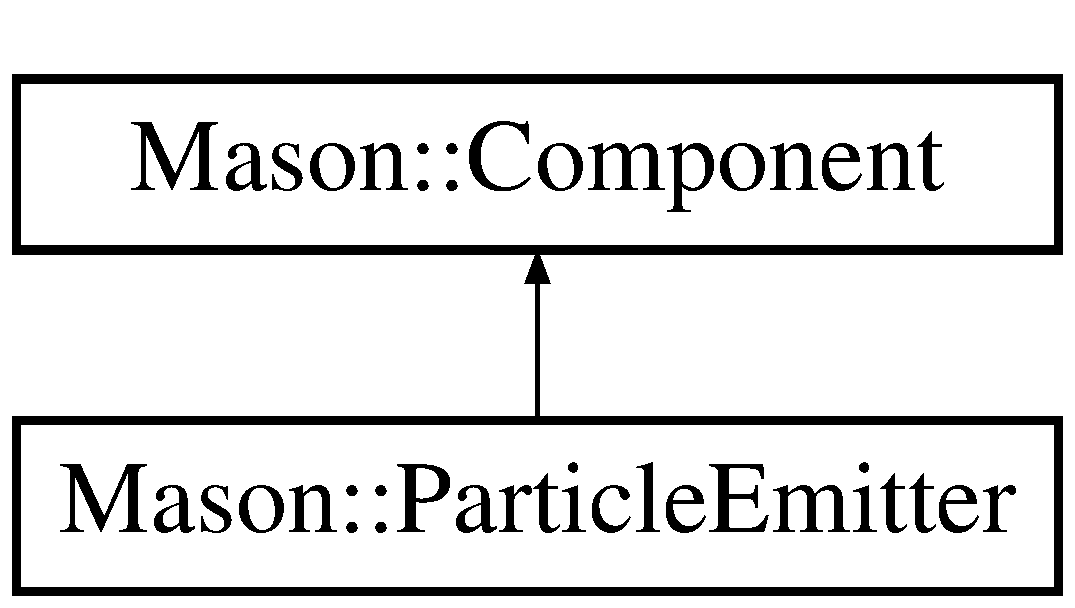
\includegraphics[height=2.000000cm]{class_mason_1_1_particle_emitter}
\end{center}
\end{figure}
\subsection*{Public Member Functions}
\begin{DoxyCompactItemize}
\item 
void \hyperlink{class_mason_1_1_particle_emitter_aa3b6ee77d7b15e2064003d8f75d53774}{render} ()
\item 
void \hyperlink{class_mason_1_1_particle_emitter_a14b63dca4ee3812ffb68f8927956683d}{clear} ()
\item 
\hyperlink{class_mason_1_1_particle_emitter_a6f4952f7555ede99d74d42b30c80f3e2}{$\sim$\+Particle\+Emitter} ()
\item 
void \hyperlink{class_mason_1_1_particle_emitter_a31dbabbe960449bcc71ac94f0421a07f}{init} (\hyperlink{struct_mason_1_1_particle_emitter_config}{Particle\+Emitter\+Config} \hyperlink{class_mason_1_1_particle_emitter_a86af1c5bfa7b301f334473b458d16ba0}{config})
\item 
void \hyperlink{class_mason_1_1_particle_emitter_a34da56b84fe4810c701f4b1541e079dc}{update} (float delta\+Time\+Sec)
\item 
void \hyperlink{class_mason_1_1_particle_emitter_aba4bcba68194e57b715779426ce68a19}{start} ()
\item 
void \hyperlink{class_mason_1_1_particle_emitter_a4843aa3afd1c4d49c9c2519837fffe81}{stop} ()
\item 
bool \hyperlink{class_mason_1_1_particle_emitter_acaf3e09e8eb747d3c603c225a781b5ff}{running} ()
\end{DoxyCompactItemize}
\subsection*{Protected Member Functions}
\begin{DoxyCompactItemize}
\item 
glm\+::vec2 \hyperlink{class_mason_1_1_particle_emitter_a9750a2b4f2f644691822b266359f1c86}{cubic\+Bezier} (float t, std\+::vector$<$ glm\+::vec2 $>$ spline\+Points)
\item 
void \hyperlink{class_mason_1_1_particle_emitter_a00459b3ebe215bede4427ad1e8e3f7dc}{update\+Model} (float delta\+Time\+Sec)
\item 
\hyperlink{class_mason_1_1_particle_emitter_a6a985b19a4f37f242030afe2c8cc5545}{Particle\+Emitter} (std\+::shared\+\_\+ptr$<$ \hyperlink{class_mason_1_1_game_object}{Game\+Object} $>$ \hyperlink{class_mason_1_1_component_abaa67b569d0a70e26a4606f4a099a925}{game\+Object})
\end{DoxyCompactItemize}
\subsection*{Protected Attributes}
\begin{DoxyCompactItemize}
\item 
S\+R\+E\+::\+Particle\+Mesh $\ast$ \hyperlink{class_mason_1_1_particle_emitter_ab144b5872ad3b63652f8a079069f4cd0}{mesh} = nullptr
\item 
S\+R\+E\+::\+Shader $\ast$ \hyperlink{class_mason_1_1_particle_emitter_abd604dd44e85f836580c40bf8d147a2c}{shader} = nullptr
\item 
std\+::vector$<$ glm\+::vec3 $>$ \hyperlink{class_mason_1_1_particle_emitter_a9398d92e4bed89396c02d4c028ba3e69}{positions} = std\+::vector$<$glm\+::vec3$>$()
\item 
std\+::vector$<$ int $>$ \hyperlink{class_mason_1_1_particle_emitter_a1c66e387ee5824b69e72efe37d5ce850}{left\+Alive} = std\+::vector$<$int$>$()
\item 
std\+::vector$<$ float $>$ \hyperlink{class_mason_1_1_particle_emitter_a6209f3a86719de038574edafc0eaa194}{sizes} = std\+::vector$<$float$>$()
\item 
std\+::vector$<$ glm\+::vec4 $>$ \hyperlink{class_mason_1_1_particle_emitter_a18c989ce7de75ba90f2b9f40f36beed1}{colors} = std\+::vector$<$glm\+::vec4$>$()
\item 
std\+::vector$<$ glm\+::vec2 $>$ \hyperlink{class_mason_1_1_particle_emitter_a6979395fb93878859edace9ab327dcc4}{uvs} = std\+::vector$<$glm\+::vec2$>$()
\item 
std\+::vector$<$ float $>$ \hyperlink{class_mason_1_1_particle_emitter_a9c2a9f3d9c113d2503598551c992fde4}{uv\+Size} = std\+::vector$<$float$>$()
\item 
std\+::vector$<$ float $>$ \hyperlink{class_mason_1_1_particle_emitter_a477934ce692453792d8be3ff51a3d22f}{uv\+Rotation} = std\+::vector$<$float$>$()
\item 
int \hyperlink{class_mason_1_1_particle_emitter_afc99ceabe0f61e289bc7e6d4c3b1b038}{total\+Particles} = 0
\item 
std\+::vector$<$ float $>$ \hyperlink{class_mason_1_1_particle_emitter_a00b9492ad2e49d6f95e05ea7c4052a57}{ages} = std\+::vector$<$float$>$()
\item 
std\+::vector$<$ glm\+::vec3 $>$ \hyperlink{class_mason_1_1_particle_emitter_aa72403d590c4528e1a1d9dbf4bc3dfd3}{velocities} = std\+::vector$<$glm\+::vec3$>$()
\item 
\hyperlink{struct_mason_1_1_particle_emitter_config}{Particle\+Emitter\+Config} \hyperlink{class_mason_1_1_particle_emitter_a86af1c5bfa7b301f334473b458d16ba0}{config}
\item 
int \hyperlink{class_mason_1_1_particle_emitter_a2df785f58db33ede9255ba835e955e11}{num\+Particles}
\item 
int \hyperlink{class_mason_1_1_particle_emitter_a591a7ed2fc6cded5dc19b144ece7b3fb}{max\+Particles}
\item 
int \hyperlink{class_mason_1_1_particle_emitter_a76a3eb861adfec2123479be32c66999c}{body\+Count} = 0
\item 
float \hyperlink{class_mason_1_1_particle_emitter_a5ae9088b02fdfd269dfd34c2a092e384}{run\+Time} = 0
\item 
float \hyperlink{class_mason_1_1_particle_emitter_a46d4d3d2871daba6f320dfbc1f89ace1}{start\+Time} = -\/1
\item 
float \hyperlink{class_mason_1_1_particle_emitter_a63333da2d5eb945d62e428f980c27523}{stop\+Time}
\item 
float \hyperlink{class_mason_1_1_particle_emitter_a79acae3c8f64f592e8868cb166b1a1ce}{last\+Update\+Time} = 0
\item 
bool \hyperlink{class_mason_1_1_particle_emitter_a615f89f70c414781aa518c8a035312bb}{emit\+New\+Particles} = false
\end{DoxyCompactItemize}
\subsection*{Friends}
\begin{DoxyCompactItemize}
\item 
class \hyperlink{class_mason_1_1_particle_emitter_a00df87c957d8f7ee0fc51f07a0542f4a}{Game\+Object}
\end{DoxyCompactItemize}


\subsection{Constructor \& Destructor Documentation}
\hypertarget{class_mason_1_1_particle_emitter_a6f4952f7555ede99d74d42b30c80f3e2}{}\label{class_mason_1_1_particle_emitter_a6f4952f7555ede99d74d42b30c80f3e2} 
\index{Mason\+::\+Particle\+Emitter@{Mason\+::\+Particle\+Emitter}!````~Particle\+Emitter@{$\sim$\+Particle\+Emitter}}
\index{````~Particle\+Emitter@{$\sim$\+Particle\+Emitter}!Mason\+::\+Particle\+Emitter@{Mason\+::\+Particle\+Emitter}}
\subsubsection{\texorpdfstring{$\sim$\+Particle\+Emitter()}{~ParticleEmitter()}}
{\footnotesize\ttfamily Particle\+Emitter\+::$\sim$\+Particle\+Emitter (\begin{DoxyParamCaption}{ }\end{DoxyParamCaption})}

\hypertarget{class_mason_1_1_particle_emitter_a6a985b19a4f37f242030afe2c8cc5545}{}\label{class_mason_1_1_particle_emitter_a6a985b19a4f37f242030afe2c8cc5545} 
\index{Mason\+::\+Particle\+Emitter@{Mason\+::\+Particle\+Emitter}!Particle\+Emitter@{Particle\+Emitter}}
\index{Particle\+Emitter@{Particle\+Emitter}!Mason\+::\+Particle\+Emitter@{Mason\+::\+Particle\+Emitter}}
\subsubsection{\texorpdfstring{Particle\+Emitter()}{ParticleEmitter()}}
{\footnotesize\ttfamily Particle\+Emitter\+::\+Particle\+Emitter (\begin{DoxyParamCaption}\item[{std\+::shared\+\_\+ptr$<$ \hyperlink{class_mason_1_1_game_object}{Game\+Object} $>$}]{game\+Object }\end{DoxyParamCaption})\hspace{0.3cm}{\ttfamily [protected]}}



\subsection{Member Function Documentation}
\hypertarget{class_mason_1_1_particle_emitter_a14b63dca4ee3812ffb68f8927956683d}{}\label{class_mason_1_1_particle_emitter_a14b63dca4ee3812ffb68f8927956683d} 
\index{Mason\+::\+Particle\+Emitter@{Mason\+::\+Particle\+Emitter}!clear@{clear}}
\index{clear@{clear}!Mason\+::\+Particle\+Emitter@{Mason\+::\+Particle\+Emitter}}
\subsubsection{\texorpdfstring{clear()}{clear()}}
{\footnotesize\ttfamily void Particle\+Emitter\+::clear (\begin{DoxyParamCaption}{ }\end{DoxyParamCaption})}

\hypertarget{class_mason_1_1_particle_emitter_a9750a2b4f2f644691822b266359f1c86}{}\label{class_mason_1_1_particle_emitter_a9750a2b4f2f644691822b266359f1c86} 
\index{Mason\+::\+Particle\+Emitter@{Mason\+::\+Particle\+Emitter}!cubic\+Bezier@{cubic\+Bezier}}
\index{cubic\+Bezier@{cubic\+Bezier}!Mason\+::\+Particle\+Emitter@{Mason\+::\+Particle\+Emitter}}
\subsubsection{\texorpdfstring{cubic\+Bezier()}{cubicBezier()}}
{\footnotesize\ttfamily glm\+::vec2 Particle\+Emitter\+::cubic\+Bezier (\begin{DoxyParamCaption}\item[{float}]{t,  }\item[{std\+::vector$<$ glm\+::vec2 $>$}]{spline\+Points }\end{DoxyParamCaption})\hspace{0.3cm}{\ttfamily [protected]}}

\hypertarget{class_mason_1_1_particle_emitter_a31dbabbe960449bcc71ac94f0421a07f}{}\label{class_mason_1_1_particle_emitter_a31dbabbe960449bcc71ac94f0421a07f} 
\index{Mason\+::\+Particle\+Emitter@{Mason\+::\+Particle\+Emitter}!init@{init}}
\index{init@{init}!Mason\+::\+Particle\+Emitter@{Mason\+::\+Particle\+Emitter}}
\subsubsection{\texorpdfstring{init()}{init()}}
{\footnotesize\ttfamily void Particle\+Emitter\+::init (\begin{DoxyParamCaption}\item[{\hyperlink{struct_mason_1_1_particle_emitter_config}{Particle\+Emitter\+Config}}]{config }\end{DoxyParamCaption})}

\hypertarget{class_mason_1_1_particle_emitter_aa3b6ee77d7b15e2064003d8f75d53774}{}\label{class_mason_1_1_particle_emitter_aa3b6ee77d7b15e2064003d8f75d53774} 
\index{Mason\+::\+Particle\+Emitter@{Mason\+::\+Particle\+Emitter}!render@{render}}
\index{render@{render}!Mason\+::\+Particle\+Emitter@{Mason\+::\+Particle\+Emitter}}
\subsubsection{\texorpdfstring{render()}{render()}}
{\footnotesize\ttfamily void Particle\+Emitter\+::render (\begin{DoxyParamCaption}{ }\end{DoxyParamCaption})}

\hypertarget{class_mason_1_1_particle_emitter_acaf3e09e8eb747d3c603c225a781b5ff}{}\label{class_mason_1_1_particle_emitter_acaf3e09e8eb747d3c603c225a781b5ff} 
\index{Mason\+::\+Particle\+Emitter@{Mason\+::\+Particle\+Emitter}!running@{running}}
\index{running@{running}!Mason\+::\+Particle\+Emitter@{Mason\+::\+Particle\+Emitter}}
\subsubsection{\texorpdfstring{running()}{running()}}
{\footnotesize\ttfamily bool Particle\+Emitter\+::running (\begin{DoxyParamCaption}{ }\end{DoxyParamCaption})}

\hypertarget{class_mason_1_1_particle_emitter_aba4bcba68194e57b715779426ce68a19}{}\label{class_mason_1_1_particle_emitter_aba4bcba68194e57b715779426ce68a19} 
\index{Mason\+::\+Particle\+Emitter@{Mason\+::\+Particle\+Emitter}!start@{start}}
\index{start@{start}!Mason\+::\+Particle\+Emitter@{Mason\+::\+Particle\+Emitter}}
\subsubsection{\texorpdfstring{start()}{start()}}
{\footnotesize\ttfamily void Particle\+Emitter\+::start (\begin{DoxyParamCaption}{ }\end{DoxyParamCaption})}

\hypertarget{class_mason_1_1_particle_emitter_a4843aa3afd1c4d49c9c2519837fffe81}{}\label{class_mason_1_1_particle_emitter_a4843aa3afd1c4d49c9c2519837fffe81} 
\index{Mason\+::\+Particle\+Emitter@{Mason\+::\+Particle\+Emitter}!stop@{stop}}
\index{stop@{stop}!Mason\+::\+Particle\+Emitter@{Mason\+::\+Particle\+Emitter}}
\subsubsection{\texorpdfstring{stop()}{stop()}}
{\footnotesize\ttfamily void Particle\+Emitter\+::stop (\begin{DoxyParamCaption}{ }\end{DoxyParamCaption})}

\hypertarget{class_mason_1_1_particle_emitter_a34da56b84fe4810c701f4b1541e079dc}{}\label{class_mason_1_1_particle_emitter_a34da56b84fe4810c701f4b1541e079dc} 
\index{Mason\+::\+Particle\+Emitter@{Mason\+::\+Particle\+Emitter}!update@{update}}
\index{update@{update}!Mason\+::\+Particle\+Emitter@{Mason\+::\+Particle\+Emitter}}
\subsubsection{\texorpdfstring{update()}{update()}}
{\footnotesize\ttfamily void Particle\+Emitter\+::update (\begin{DoxyParamCaption}\item[{float}]{delta\+Time\+Sec }\end{DoxyParamCaption})}

\hypertarget{class_mason_1_1_particle_emitter_a00459b3ebe215bede4427ad1e8e3f7dc}{}\label{class_mason_1_1_particle_emitter_a00459b3ebe215bede4427ad1e8e3f7dc} 
\index{Mason\+::\+Particle\+Emitter@{Mason\+::\+Particle\+Emitter}!update\+Model@{update\+Model}}
\index{update\+Model@{update\+Model}!Mason\+::\+Particle\+Emitter@{Mason\+::\+Particle\+Emitter}}
\subsubsection{\texorpdfstring{update\+Model()}{updateModel()}}
{\footnotesize\ttfamily void Particle\+Emitter\+::update\+Model (\begin{DoxyParamCaption}\item[{float}]{delta\+Time\+Sec }\end{DoxyParamCaption})\hspace{0.3cm}{\ttfamily [protected]}}



\subsection{Friends And Related Function Documentation}
\hypertarget{class_mason_1_1_particle_emitter_a00df87c957d8f7ee0fc51f07a0542f4a}{}\label{class_mason_1_1_particle_emitter_a00df87c957d8f7ee0fc51f07a0542f4a} 
\index{Mason\+::\+Particle\+Emitter@{Mason\+::\+Particle\+Emitter}!Game\+Object@{Game\+Object}}
\index{Game\+Object@{Game\+Object}!Mason\+::\+Particle\+Emitter@{Mason\+::\+Particle\+Emitter}}
\subsubsection{\texorpdfstring{Game\+Object}{GameObject}}
{\footnotesize\ttfamily friend class \hyperlink{class_mason_1_1_game_object}{Game\+Object}\hspace{0.3cm}{\ttfamily [friend]}}



\subsection{Member Data Documentation}
\hypertarget{class_mason_1_1_particle_emitter_a00b9492ad2e49d6f95e05ea7c4052a57}{}\label{class_mason_1_1_particle_emitter_a00b9492ad2e49d6f95e05ea7c4052a57} 
\index{Mason\+::\+Particle\+Emitter@{Mason\+::\+Particle\+Emitter}!ages@{ages}}
\index{ages@{ages}!Mason\+::\+Particle\+Emitter@{Mason\+::\+Particle\+Emitter}}
\subsubsection{\texorpdfstring{ages}{ages}}
{\footnotesize\ttfamily std\+::vector$<$float$>$ Mason\+::\+Particle\+Emitter\+::ages = std\+::vector$<$float$>$()\hspace{0.3cm}{\ttfamily [protected]}}

\hypertarget{class_mason_1_1_particle_emitter_a76a3eb861adfec2123479be32c66999c}{}\label{class_mason_1_1_particle_emitter_a76a3eb861adfec2123479be32c66999c} 
\index{Mason\+::\+Particle\+Emitter@{Mason\+::\+Particle\+Emitter}!body\+Count@{body\+Count}}
\index{body\+Count@{body\+Count}!Mason\+::\+Particle\+Emitter@{Mason\+::\+Particle\+Emitter}}
\subsubsection{\texorpdfstring{body\+Count}{bodyCount}}
{\footnotesize\ttfamily int Mason\+::\+Particle\+Emitter\+::body\+Count = 0\hspace{0.3cm}{\ttfamily [protected]}}

\hypertarget{class_mason_1_1_particle_emitter_a18c989ce7de75ba90f2b9f40f36beed1}{}\label{class_mason_1_1_particle_emitter_a18c989ce7de75ba90f2b9f40f36beed1} 
\index{Mason\+::\+Particle\+Emitter@{Mason\+::\+Particle\+Emitter}!colors@{colors}}
\index{colors@{colors}!Mason\+::\+Particle\+Emitter@{Mason\+::\+Particle\+Emitter}}
\subsubsection{\texorpdfstring{colors}{colors}}
{\footnotesize\ttfamily std\+::vector$<$glm\+::vec4$>$ Mason\+::\+Particle\+Emitter\+::colors = std\+::vector$<$glm\+::vec4$>$()\hspace{0.3cm}{\ttfamily [protected]}}

\hypertarget{class_mason_1_1_particle_emitter_a86af1c5bfa7b301f334473b458d16ba0}{}\label{class_mason_1_1_particle_emitter_a86af1c5bfa7b301f334473b458d16ba0} 
\index{Mason\+::\+Particle\+Emitter@{Mason\+::\+Particle\+Emitter}!config@{config}}
\index{config@{config}!Mason\+::\+Particle\+Emitter@{Mason\+::\+Particle\+Emitter}}
\subsubsection{\texorpdfstring{config}{config}}
{\footnotesize\ttfamily \hyperlink{struct_mason_1_1_particle_emitter_config}{Particle\+Emitter\+Config} Mason\+::\+Particle\+Emitter\+::config\hspace{0.3cm}{\ttfamily [protected]}}

\hypertarget{class_mason_1_1_particle_emitter_a615f89f70c414781aa518c8a035312bb}{}\label{class_mason_1_1_particle_emitter_a615f89f70c414781aa518c8a035312bb} 
\index{Mason\+::\+Particle\+Emitter@{Mason\+::\+Particle\+Emitter}!emit\+New\+Particles@{emit\+New\+Particles}}
\index{emit\+New\+Particles@{emit\+New\+Particles}!Mason\+::\+Particle\+Emitter@{Mason\+::\+Particle\+Emitter}}
\subsubsection{\texorpdfstring{emit\+New\+Particles}{emitNewParticles}}
{\footnotesize\ttfamily bool Mason\+::\+Particle\+Emitter\+::emit\+New\+Particles = false\hspace{0.3cm}{\ttfamily [protected]}}

\hypertarget{class_mason_1_1_particle_emitter_a79acae3c8f64f592e8868cb166b1a1ce}{}\label{class_mason_1_1_particle_emitter_a79acae3c8f64f592e8868cb166b1a1ce} 
\index{Mason\+::\+Particle\+Emitter@{Mason\+::\+Particle\+Emitter}!last\+Update\+Time@{last\+Update\+Time}}
\index{last\+Update\+Time@{last\+Update\+Time}!Mason\+::\+Particle\+Emitter@{Mason\+::\+Particle\+Emitter}}
\subsubsection{\texorpdfstring{last\+Update\+Time}{lastUpdateTime}}
{\footnotesize\ttfamily float Mason\+::\+Particle\+Emitter\+::last\+Update\+Time = 0\hspace{0.3cm}{\ttfamily [protected]}}

\hypertarget{class_mason_1_1_particle_emitter_a1c66e387ee5824b69e72efe37d5ce850}{}\label{class_mason_1_1_particle_emitter_a1c66e387ee5824b69e72efe37d5ce850} 
\index{Mason\+::\+Particle\+Emitter@{Mason\+::\+Particle\+Emitter}!left\+Alive@{left\+Alive}}
\index{left\+Alive@{left\+Alive}!Mason\+::\+Particle\+Emitter@{Mason\+::\+Particle\+Emitter}}
\subsubsection{\texorpdfstring{left\+Alive}{leftAlive}}
{\footnotesize\ttfamily std\+::vector$<$int$>$ Mason\+::\+Particle\+Emitter\+::left\+Alive = std\+::vector$<$int$>$()\hspace{0.3cm}{\ttfamily [protected]}}

\hypertarget{class_mason_1_1_particle_emitter_a591a7ed2fc6cded5dc19b144ece7b3fb}{}\label{class_mason_1_1_particle_emitter_a591a7ed2fc6cded5dc19b144ece7b3fb} 
\index{Mason\+::\+Particle\+Emitter@{Mason\+::\+Particle\+Emitter}!max\+Particles@{max\+Particles}}
\index{max\+Particles@{max\+Particles}!Mason\+::\+Particle\+Emitter@{Mason\+::\+Particle\+Emitter}}
\subsubsection{\texorpdfstring{max\+Particles}{maxParticles}}
{\footnotesize\ttfamily int Mason\+::\+Particle\+Emitter\+::max\+Particles\hspace{0.3cm}{\ttfamily [protected]}}

\hypertarget{class_mason_1_1_particle_emitter_ab144b5872ad3b63652f8a079069f4cd0}{}\label{class_mason_1_1_particle_emitter_ab144b5872ad3b63652f8a079069f4cd0} 
\index{Mason\+::\+Particle\+Emitter@{Mason\+::\+Particle\+Emitter}!mesh@{mesh}}
\index{mesh@{mesh}!Mason\+::\+Particle\+Emitter@{Mason\+::\+Particle\+Emitter}}
\subsubsection{\texorpdfstring{mesh}{mesh}}
{\footnotesize\ttfamily S\+R\+E\+::\+Particle\+Mesh$\ast$ Mason\+::\+Particle\+Emitter\+::mesh = nullptr\hspace{0.3cm}{\ttfamily [protected]}}

\hypertarget{class_mason_1_1_particle_emitter_a2df785f58db33ede9255ba835e955e11}{}\label{class_mason_1_1_particle_emitter_a2df785f58db33ede9255ba835e955e11} 
\index{Mason\+::\+Particle\+Emitter@{Mason\+::\+Particle\+Emitter}!num\+Particles@{num\+Particles}}
\index{num\+Particles@{num\+Particles}!Mason\+::\+Particle\+Emitter@{Mason\+::\+Particle\+Emitter}}
\subsubsection{\texorpdfstring{num\+Particles}{numParticles}}
{\footnotesize\ttfamily int Mason\+::\+Particle\+Emitter\+::num\+Particles\hspace{0.3cm}{\ttfamily [protected]}}

\hypertarget{class_mason_1_1_particle_emitter_a9398d92e4bed89396c02d4c028ba3e69}{}\label{class_mason_1_1_particle_emitter_a9398d92e4bed89396c02d4c028ba3e69} 
\index{Mason\+::\+Particle\+Emitter@{Mason\+::\+Particle\+Emitter}!positions@{positions}}
\index{positions@{positions}!Mason\+::\+Particle\+Emitter@{Mason\+::\+Particle\+Emitter}}
\subsubsection{\texorpdfstring{positions}{positions}}
{\footnotesize\ttfamily std\+::vector$<$glm\+::vec3$>$ Mason\+::\+Particle\+Emitter\+::positions = std\+::vector$<$glm\+::vec3$>$()\hspace{0.3cm}{\ttfamily [protected]}}

\hypertarget{class_mason_1_1_particle_emitter_a5ae9088b02fdfd269dfd34c2a092e384}{}\label{class_mason_1_1_particle_emitter_a5ae9088b02fdfd269dfd34c2a092e384} 
\index{Mason\+::\+Particle\+Emitter@{Mason\+::\+Particle\+Emitter}!run\+Time@{run\+Time}}
\index{run\+Time@{run\+Time}!Mason\+::\+Particle\+Emitter@{Mason\+::\+Particle\+Emitter}}
\subsubsection{\texorpdfstring{run\+Time}{runTime}}
{\footnotesize\ttfamily float Mason\+::\+Particle\+Emitter\+::run\+Time = 0\hspace{0.3cm}{\ttfamily [protected]}}

\hypertarget{class_mason_1_1_particle_emitter_abd604dd44e85f836580c40bf8d147a2c}{}\label{class_mason_1_1_particle_emitter_abd604dd44e85f836580c40bf8d147a2c} 
\index{Mason\+::\+Particle\+Emitter@{Mason\+::\+Particle\+Emitter}!shader@{shader}}
\index{shader@{shader}!Mason\+::\+Particle\+Emitter@{Mason\+::\+Particle\+Emitter}}
\subsubsection{\texorpdfstring{shader}{shader}}
{\footnotesize\ttfamily S\+R\+E\+::\+Shader$\ast$ Mason\+::\+Particle\+Emitter\+::shader = nullptr\hspace{0.3cm}{\ttfamily [protected]}}

\hypertarget{class_mason_1_1_particle_emitter_a6209f3a86719de038574edafc0eaa194}{}\label{class_mason_1_1_particle_emitter_a6209f3a86719de038574edafc0eaa194} 
\index{Mason\+::\+Particle\+Emitter@{Mason\+::\+Particle\+Emitter}!sizes@{sizes}}
\index{sizes@{sizes}!Mason\+::\+Particle\+Emitter@{Mason\+::\+Particle\+Emitter}}
\subsubsection{\texorpdfstring{sizes}{sizes}}
{\footnotesize\ttfamily std\+::vector$<$float$>$ Mason\+::\+Particle\+Emitter\+::sizes = std\+::vector$<$float$>$()\hspace{0.3cm}{\ttfamily [protected]}}

\hypertarget{class_mason_1_1_particle_emitter_a46d4d3d2871daba6f320dfbc1f89ace1}{}\label{class_mason_1_1_particle_emitter_a46d4d3d2871daba6f320dfbc1f89ace1} 
\index{Mason\+::\+Particle\+Emitter@{Mason\+::\+Particle\+Emitter}!start\+Time@{start\+Time}}
\index{start\+Time@{start\+Time}!Mason\+::\+Particle\+Emitter@{Mason\+::\+Particle\+Emitter}}
\subsubsection{\texorpdfstring{start\+Time}{startTime}}
{\footnotesize\ttfamily float Mason\+::\+Particle\+Emitter\+::start\+Time = -\/1\hspace{0.3cm}{\ttfamily [protected]}}

\hypertarget{class_mason_1_1_particle_emitter_a63333da2d5eb945d62e428f980c27523}{}\label{class_mason_1_1_particle_emitter_a63333da2d5eb945d62e428f980c27523} 
\index{Mason\+::\+Particle\+Emitter@{Mason\+::\+Particle\+Emitter}!stop\+Time@{stop\+Time}}
\index{stop\+Time@{stop\+Time}!Mason\+::\+Particle\+Emitter@{Mason\+::\+Particle\+Emitter}}
\subsubsection{\texorpdfstring{stop\+Time}{stopTime}}
{\footnotesize\ttfamily float Mason\+::\+Particle\+Emitter\+::stop\+Time\hspace{0.3cm}{\ttfamily [protected]}}

\hypertarget{class_mason_1_1_particle_emitter_afc99ceabe0f61e289bc7e6d4c3b1b038}{}\label{class_mason_1_1_particle_emitter_afc99ceabe0f61e289bc7e6d4c3b1b038} 
\index{Mason\+::\+Particle\+Emitter@{Mason\+::\+Particle\+Emitter}!total\+Particles@{total\+Particles}}
\index{total\+Particles@{total\+Particles}!Mason\+::\+Particle\+Emitter@{Mason\+::\+Particle\+Emitter}}
\subsubsection{\texorpdfstring{total\+Particles}{totalParticles}}
{\footnotesize\ttfamily int Mason\+::\+Particle\+Emitter\+::total\+Particles = 0\hspace{0.3cm}{\ttfamily [protected]}}

\hypertarget{class_mason_1_1_particle_emitter_a477934ce692453792d8be3ff51a3d22f}{}\label{class_mason_1_1_particle_emitter_a477934ce692453792d8be3ff51a3d22f} 
\index{Mason\+::\+Particle\+Emitter@{Mason\+::\+Particle\+Emitter}!uv\+Rotation@{uv\+Rotation}}
\index{uv\+Rotation@{uv\+Rotation}!Mason\+::\+Particle\+Emitter@{Mason\+::\+Particle\+Emitter}}
\subsubsection{\texorpdfstring{uv\+Rotation}{uvRotation}}
{\footnotesize\ttfamily std\+::vector$<$float$>$ Mason\+::\+Particle\+Emitter\+::uv\+Rotation = std\+::vector$<$float$>$()\hspace{0.3cm}{\ttfamily [protected]}}

\hypertarget{class_mason_1_1_particle_emitter_a6979395fb93878859edace9ab327dcc4}{}\label{class_mason_1_1_particle_emitter_a6979395fb93878859edace9ab327dcc4} 
\index{Mason\+::\+Particle\+Emitter@{Mason\+::\+Particle\+Emitter}!uvs@{uvs}}
\index{uvs@{uvs}!Mason\+::\+Particle\+Emitter@{Mason\+::\+Particle\+Emitter}}
\subsubsection{\texorpdfstring{uvs}{uvs}}
{\footnotesize\ttfamily std\+::vector$<$glm\+::vec2$>$ Mason\+::\+Particle\+Emitter\+::uvs = std\+::vector$<$glm\+::vec2$>$()\hspace{0.3cm}{\ttfamily [protected]}}

\hypertarget{class_mason_1_1_particle_emitter_a9c2a9f3d9c113d2503598551c992fde4}{}\label{class_mason_1_1_particle_emitter_a9c2a9f3d9c113d2503598551c992fde4} 
\index{Mason\+::\+Particle\+Emitter@{Mason\+::\+Particle\+Emitter}!uv\+Size@{uv\+Size}}
\index{uv\+Size@{uv\+Size}!Mason\+::\+Particle\+Emitter@{Mason\+::\+Particle\+Emitter}}
\subsubsection{\texorpdfstring{uv\+Size}{uvSize}}
{\footnotesize\ttfamily std\+::vector$<$float$>$ Mason\+::\+Particle\+Emitter\+::uv\+Size = std\+::vector$<$float$>$()\hspace{0.3cm}{\ttfamily [protected]}}

\hypertarget{class_mason_1_1_particle_emitter_aa72403d590c4528e1a1d9dbf4bc3dfd3}{}\label{class_mason_1_1_particle_emitter_aa72403d590c4528e1a1d9dbf4bc3dfd3} 
\index{Mason\+::\+Particle\+Emitter@{Mason\+::\+Particle\+Emitter}!velocities@{velocities}}
\index{velocities@{velocities}!Mason\+::\+Particle\+Emitter@{Mason\+::\+Particle\+Emitter}}
\subsubsection{\texorpdfstring{velocities}{velocities}}
{\footnotesize\ttfamily std\+::vector$<$glm\+::vec3$>$ Mason\+::\+Particle\+Emitter\+::velocities = std\+::vector$<$glm\+::vec3$>$()\hspace{0.3cm}{\ttfamily [protected]}}



The documentation for this class was generated from the following files\+:\begin{DoxyCompactItemize}
\item 
include/\+Mason/\hyperlink{_particle_emitter_8hpp}{Particle\+Emitter.\+hpp}\item 
src/\hyperlink{_particle_emitter_8cpp}{Particle\+Emitter.\+cpp}\end{DoxyCompactItemize}

\hypertarget{struct_mason_1_1_particle_emitter_config}{}\section{Mason\+:\+:Particle\+Emitter\+Config Struct Reference}
\label{struct_mason_1_1_particle_emitter_config}\index{Mason\+::\+Particle\+Emitter\+Config@{Mason\+::\+Particle\+Emitter\+Config}}


{\ttfamily \#include $<$Particle\+Emitter.\+hpp$>$}

\subsection*{Public Member Functions}
\begin{DoxyCompactItemize}
\item 
\hyperlink{namespace_mason_aefc2ce7d9295b57af46ab6c8ebfc32f7}{Attribute\+State} \hyperlink{struct_mason_1_1_particle_emitter_config_a9ee7a40d6337225cccab9f801e8f793f}{attribute\+From\+String} (std\+::string str)
\item 
std\+::vector$<$ glm\+::vec2 $>$ \hyperlink{struct_mason_1_1_particle_emitter_config_ae3781dff36d32c1fb79a8ff63baf2c55}{normalize} (std\+::vector$<$ glm\+::vec2 $>$ input)
\item 
void \hyperlink{struct_mason_1_1_particle_emitter_config_a92978f0e01ba1078889a3f288ff0c02b}{set\+Texture} (S\+R\+E\+::\+Texture $\ast$\+\_\+tex)
\item 
void \hyperlink{struct_mason_1_1_particle_emitter_config_a8569c3e45131fd9d51687bbf293e3154}{set\+Rate} (float \+\_\+rate)
\item 
void \hyperlink{struct_mason_1_1_particle_emitter_config_afe91ca5c2d60e5567fe589367b4fd3ef}{set\+Lifespan} (float \+\_\+lifespan)
\item 
void \hyperlink{struct_mason_1_1_particle_emitter_config_ae5eafd4808934831fb271304c24b6af7}{set\+Velocity} (glm\+::vec3 \+\_\+velocity)
\item 
void \hyperlink{struct_mason_1_1_particle_emitter_config_ab34a3cc0d4c7252492a261c063b9376b}{set\+Gravity} (glm\+::vec3 \+\_\+gravity)
\item 
void \hyperlink{struct_mason_1_1_particle_emitter_config_a63a5b2c01c1f4cc0eaa1e8d4b9226146}{set\+Fixed\+Velocity} (glm\+::vec3 vel)
\item 
void \hyperlink{struct_mason_1_1_particle_emitter_config_a9102ce5287cd4c13e89f5e695563076f}{set\+Random\+Velocity} (glm\+::vec3 min\+Vel, glm\+::vec3 max\+Vel)
\item 
void \hyperlink{struct_mason_1_1_particle_emitter_config_a52313455114fadb6609232719681b4d7}{set\+Fixed\+Size} (float size)
\item 
void \hyperlink{struct_mason_1_1_particle_emitter_config_ab644fd902c0e29f758a53912d0784f19}{set\+Random\+Size} (float min, float max)
\item 
void \hyperlink{struct_mason_1_1_particle_emitter_config_a5495ec9be73c80df30115461b6af7733}{set\+L\+E\+R\+P\+Size} (float initial, float final)
\item 
void \hyperlink{struct_mason_1_1_particle_emitter_config_a4288325ce9dcf3437fbcabaf99f968b4}{set\+Spline\+Interp\+Size} (float initial, float final, std\+::vector$<$ glm\+::vec2 $>$ spline\+Points)
\item 
void \hyperlink{struct_mason_1_1_particle_emitter_config_ae4aa09d5feb556808fba6c23167d9d78}{set\+Fixed\+Color} (glm\+::vec4 color)
\item 
void \hyperlink{struct_mason_1_1_particle_emitter_config_a5317af2f90691360678a2663a747c36d}{set\+Random\+Color} (glm\+::vec4 min, glm\+::vec4 max)
\item 
void \hyperlink{struct_mason_1_1_particle_emitter_config_a09620b4edcadd022cd8a447da17867a0}{set\+L\+E\+R\+P\+Color} (glm\+::vec4 initial, glm\+::vec4 final)
\item 
void \hyperlink{struct_mason_1_1_particle_emitter_config_aaf515319a62060a75edbb1e7b6403ff2}{set\+Spline\+Interp\+Color} (glm\+::vec4 initial, glm\+::vec4 final, std\+::vector$<$ glm\+::vec2 $>$ spline\+Points)
\item 
void \hyperlink{struct_mason_1_1_particle_emitter_config_acb790846d2a00fd97160fdac66589fd5}{set\+Fixed\+Rotation} (float rotation)
\item 
void \hyperlink{struct_mason_1_1_particle_emitter_config_a463adb67fe4ee1732daa20e9d01d2331}{set\+Random\+Rotation} (float min, float max)
\item 
void \hyperlink{struct_mason_1_1_particle_emitter_config_ad96c857c3ceac520462a10981e471c4b}{set\+L\+E\+R\+P\+Rotation} (float initial, float final)
\item 
void \hyperlink{struct_mason_1_1_particle_emitter_config_abcaf3368ccf9b524538a3cf3fadb15d2}{set\+Spline\+Interp\+Rotation} (float initial, float final, std\+::vector$<$ glm\+::vec2 $>$ spline\+Points)
\item 
\hyperlink{struct_mason_1_1_particle_emitter_config_a317aa2e9d325160e20fd1bbefdc244f5}{Particle\+Emitter\+Config} ()
\item 
\hyperlink{struct_mason_1_1_particle_emitter_config_a50ce1e6e4420674c75b12b402ac5bf33}{Particle\+Emitter\+Config} (float \hyperlink{struct_mason_1_1_particle_emitter_config_abc0c7231f9134e3b0456d22ee8d5c8a2}{rate}, float \hyperlink{struct_mason_1_1_particle_emitter_config_a856b3906e25a7d41eb9bc7e37a91ef93}{lifespan}, glm\+::vec3 \hyperlink{struct_mason_1_1_particle_emitter_config_af8c3efa305e0a0636576bebe60938c80}{velocity}, glm\+::vec3 \hyperlink{struct_mason_1_1_particle_emitter_config_ad5fa0930e4e3f5d8c9de1324a854e63a}{gravity})
\end{DoxyCompactItemize}
\subsection*{Public Attributes}
\begin{DoxyCompactItemize}
\item 
S\+R\+E\+::\+Texture $\ast$ \hyperlink{struct_mason_1_1_particle_emitter_config_a660e9a7613b158ac36bfc4ffe8b5f610}{tex} = nullptr
\item 
float \hyperlink{struct_mason_1_1_particle_emitter_config_abc0c7231f9134e3b0456d22ee8d5c8a2}{rate}
\item 
float \hyperlink{struct_mason_1_1_particle_emitter_config_a856b3906e25a7d41eb9bc7e37a91ef93}{lifespan}
\item 
glm\+::vec3 \hyperlink{struct_mason_1_1_particle_emitter_config_af8c3efa305e0a0636576bebe60938c80}{velocity}
\item 
glm\+::vec3 \hyperlink{struct_mason_1_1_particle_emitter_config_ad5fa0930e4e3f5d8c9de1324a854e63a}{gravity}
\item 
float \hyperlink{struct_mason_1_1_particle_emitter_config_ab46ccc780e60c6b7006749058654455f}{min\+Size}
\item 
float \hyperlink{struct_mason_1_1_particle_emitter_config_ad8b8933ec9758ed264d1b1ccc3d24bd8}{max\+Size}
\item 
float \hyperlink{struct_mason_1_1_particle_emitter_config_ae6755b96da7af8b4c469b64f0887e186}{min\+Rotation}
\item 
float \hyperlink{struct_mason_1_1_particle_emitter_config_a3a7e271bae699c0998a3d9ac73f3bb6f}{max\+Rotation}
\item 
glm\+::vec4 \hyperlink{struct_mason_1_1_particle_emitter_config_aa70f6e44cc9712bf59ef89e1a339726d}{min\+Color}
\item 
glm\+::vec4 \hyperlink{struct_mason_1_1_particle_emitter_config_af48c8574b50e51408c3566f862e22dbd}{max\+Color}
\item 
glm\+::vec3 \hyperlink{struct_mason_1_1_particle_emitter_config_a3d8df085c0a91b61f42adc5eef888c79}{min\+Velocity}
\item 
glm\+::vec3 \hyperlink{struct_mason_1_1_particle_emitter_config_aa449573ac5e8ae2ef3f5110836a3091c}{max\+Velocity}
\item 
float \hyperlink{struct_mason_1_1_particle_emitter_config_a200875bdd8d24d919160527494c5b611}{initial\+Size}
\item 
float \hyperlink{struct_mason_1_1_particle_emitter_config_a5aabaa7aa8bd203539a56ee269595f94}{final\+Size}
\item 
glm\+::vec4 \hyperlink{struct_mason_1_1_particle_emitter_config_a8580419bef5f1d337f75a5224dec0deb}{initial\+Color}
\item 
glm\+::vec4 \hyperlink{struct_mason_1_1_particle_emitter_config_addf94f6df6c784495840b93aa30ce162}{final\+Color}
\item 
float \hyperlink{struct_mason_1_1_particle_emitter_config_a94e5a301870aa19cc1bf14d4613cc879}{initial\+Rotation}
\item 
float \hyperlink{struct_mason_1_1_particle_emitter_config_a37a579321019d25bdb1ecf4f32353d7c}{final\+Rotation}
\item 
std\+::vector$<$ glm\+::vec2 $>$ \hyperlink{struct_mason_1_1_particle_emitter_config_a66a4652dce73b58e27b8a495e2b6e0eb}{spline\+Points\+Color}
\item 
std\+::vector$<$ glm\+::vec2 $>$ \hyperlink{struct_mason_1_1_particle_emitter_config_ae379890e2a2de9c8f4dc1a391393f41a}{spline\+Points\+Size}
\item 
std\+::vector$<$ glm\+::vec2 $>$ \hyperlink{struct_mason_1_1_particle_emitter_config_ae03fbdb37c6738eafedc10564d744e8e}{spline\+Points\+Rotation}
\item 
\hyperlink{namespace_mason_aefc2ce7d9295b57af46ab6c8ebfc32f7}{Attribute\+State} \hyperlink{struct_mason_1_1_particle_emitter_config_a94ad732500966a699dcead307033269a}{color\+State}
\item 
\hyperlink{namespace_mason_aefc2ce7d9295b57af46ab6c8ebfc32f7}{Attribute\+State} \hyperlink{struct_mason_1_1_particle_emitter_config_a3f6f8e64ff56799d85b8512aa97801eb}{size\+State}
\item 
\hyperlink{namespace_mason_aefc2ce7d9295b57af46ab6c8ebfc32f7}{Attribute\+State} \hyperlink{struct_mason_1_1_particle_emitter_config_a35b60fea30c8a07adcfc77a3c30e1546}{rotation\+State}
\item 
\hyperlink{namespace_mason_aefc2ce7d9295b57af46ab6c8ebfc32f7}{Attribute\+State} \hyperlink{struct_mason_1_1_particle_emitter_config_a449a7ec64ad8d9f9be405f1beb5ee507}{velocity\+State}
\end{DoxyCompactItemize}


\subsection{Constructor \& Destructor Documentation}
\hypertarget{struct_mason_1_1_particle_emitter_config_a317aa2e9d325160e20fd1bbefdc244f5}{}\label{struct_mason_1_1_particle_emitter_config_a317aa2e9d325160e20fd1bbefdc244f5} 
\index{Mason\+::\+Particle\+Emitter\+Config@{Mason\+::\+Particle\+Emitter\+Config}!Particle\+Emitter\+Config@{Particle\+Emitter\+Config}}
\index{Particle\+Emitter\+Config@{Particle\+Emitter\+Config}!Mason\+::\+Particle\+Emitter\+Config@{Mason\+::\+Particle\+Emitter\+Config}}
\subsubsection{\texorpdfstring{Particle\+Emitter\+Config()}{ParticleEmitterConfig()}\hspace{0.1cm}{\footnotesize\ttfamily [1/2]}}
{\footnotesize\ttfamily Mason\+::\+Particle\+Emitter\+Config\+::\+Particle\+Emitter\+Config (\begin{DoxyParamCaption}{ }\end{DoxyParamCaption})\hspace{0.3cm}{\ttfamily [inline]}}

\hypertarget{struct_mason_1_1_particle_emitter_config_a50ce1e6e4420674c75b12b402ac5bf33}{}\label{struct_mason_1_1_particle_emitter_config_a50ce1e6e4420674c75b12b402ac5bf33} 
\index{Mason\+::\+Particle\+Emitter\+Config@{Mason\+::\+Particle\+Emitter\+Config}!Particle\+Emitter\+Config@{Particle\+Emitter\+Config}}
\index{Particle\+Emitter\+Config@{Particle\+Emitter\+Config}!Mason\+::\+Particle\+Emitter\+Config@{Mason\+::\+Particle\+Emitter\+Config}}
\subsubsection{\texorpdfstring{Particle\+Emitter\+Config()}{ParticleEmitterConfig()}\hspace{0.1cm}{\footnotesize\ttfamily [2/2]}}
{\footnotesize\ttfamily Mason\+::\+Particle\+Emitter\+Config\+::\+Particle\+Emitter\+Config (\begin{DoxyParamCaption}\item[{float}]{rate,  }\item[{float}]{lifespan,  }\item[{glm\+::vec3}]{velocity,  }\item[{glm\+::vec3}]{gravity }\end{DoxyParamCaption})\hspace{0.3cm}{\ttfamily [inline]}}



\subsection{Member Function Documentation}
\hypertarget{struct_mason_1_1_particle_emitter_config_a9ee7a40d6337225cccab9f801e8f793f}{}\label{struct_mason_1_1_particle_emitter_config_a9ee7a40d6337225cccab9f801e8f793f} 
\index{Mason\+::\+Particle\+Emitter\+Config@{Mason\+::\+Particle\+Emitter\+Config}!attribute\+From\+String@{attribute\+From\+String}}
\index{attribute\+From\+String@{attribute\+From\+String}!Mason\+::\+Particle\+Emitter\+Config@{Mason\+::\+Particle\+Emitter\+Config}}
\subsubsection{\texorpdfstring{attribute\+From\+String()}{attributeFromString()}}
{\footnotesize\ttfamily \hyperlink{namespace_mason_aefc2ce7d9295b57af46ab6c8ebfc32f7}{Attribute\+State} Mason\+::\+Particle\+Emitter\+Config\+::attribute\+From\+String (\begin{DoxyParamCaption}\item[{std\+::string}]{str }\end{DoxyParamCaption})\hspace{0.3cm}{\ttfamily [inline]}}

\hypertarget{struct_mason_1_1_particle_emitter_config_ae3781dff36d32c1fb79a8ff63baf2c55}{}\label{struct_mason_1_1_particle_emitter_config_ae3781dff36d32c1fb79a8ff63baf2c55} 
\index{Mason\+::\+Particle\+Emitter\+Config@{Mason\+::\+Particle\+Emitter\+Config}!normalize@{normalize}}
\index{normalize@{normalize}!Mason\+::\+Particle\+Emitter\+Config@{Mason\+::\+Particle\+Emitter\+Config}}
\subsubsection{\texorpdfstring{normalize()}{normalize()}}
{\footnotesize\ttfamily std\+::vector$<$glm\+::vec2$>$ Mason\+::\+Particle\+Emitter\+Config\+::normalize (\begin{DoxyParamCaption}\item[{std\+::vector$<$ glm\+::vec2 $>$}]{input }\end{DoxyParamCaption})\hspace{0.3cm}{\ttfamily [inline]}}

\hypertarget{struct_mason_1_1_particle_emitter_config_ae4aa09d5feb556808fba6c23167d9d78}{}\label{struct_mason_1_1_particle_emitter_config_ae4aa09d5feb556808fba6c23167d9d78} 
\index{Mason\+::\+Particle\+Emitter\+Config@{Mason\+::\+Particle\+Emitter\+Config}!set\+Fixed\+Color@{set\+Fixed\+Color}}
\index{set\+Fixed\+Color@{set\+Fixed\+Color}!Mason\+::\+Particle\+Emitter\+Config@{Mason\+::\+Particle\+Emitter\+Config}}
\subsubsection{\texorpdfstring{set\+Fixed\+Color()}{setFixedColor()}}
{\footnotesize\ttfamily void Mason\+::\+Particle\+Emitter\+Config\+::set\+Fixed\+Color (\begin{DoxyParamCaption}\item[{glm\+::vec4}]{color }\end{DoxyParamCaption})\hspace{0.3cm}{\ttfamily [inline]}}

\hypertarget{struct_mason_1_1_particle_emitter_config_acb790846d2a00fd97160fdac66589fd5}{}\label{struct_mason_1_1_particle_emitter_config_acb790846d2a00fd97160fdac66589fd5} 
\index{Mason\+::\+Particle\+Emitter\+Config@{Mason\+::\+Particle\+Emitter\+Config}!set\+Fixed\+Rotation@{set\+Fixed\+Rotation}}
\index{set\+Fixed\+Rotation@{set\+Fixed\+Rotation}!Mason\+::\+Particle\+Emitter\+Config@{Mason\+::\+Particle\+Emitter\+Config}}
\subsubsection{\texorpdfstring{set\+Fixed\+Rotation()}{setFixedRotation()}}
{\footnotesize\ttfamily void Mason\+::\+Particle\+Emitter\+Config\+::set\+Fixed\+Rotation (\begin{DoxyParamCaption}\item[{float}]{rotation }\end{DoxyParamCaption})\hspace{0.3cm}{\ttfamily [inline]}}

\hypertarget{struct_mason_1_1_particle_emitter_config_a52313455114fadb6609232719681b4d7}{}\label{struct_mason_1_1_particle_emitter_config_a52313455114fadb6609232719681b4d7} 
\index{Mason\+::\+Particle\+Emitter\+Config@{Mason\+::\+Particle\+Emitter\+Config}!set\+Fixed\+Size@{set\+Fixed\+Size}}
\index{set\+Fixed\+Size@{set\+Fixed\+Size}!Mason\+::\+Particle\+Emitter\+Config@{Mason\+::\+Particle\+Emitter\+Config}}
\subsubsection{\texorpdfstring{set\+Fixed\+Size()}{setFixedSize()}}
{\footnotesize\ttfamily void Mason\+::\+Particle\+Emitter\+Config\+::set\+Fixed\+Size (\begin{DoxyParamCaption}\item[{float}]{size }\end{DoxyParamCaption})\hspace{0.3cm}{\ttfamily [inline]}}

\hypertarget{struct_mason_1_1_particle_emitter_config_a63a5b2c01c1f4cc0eaa1e8d4b9226146}{}\label{struct_mason_1_1_particle_emitter_config_a63a5b2c01c1f4cc0eaa1e8d4b9226146} 
\index{Mason\+::\+Particle\+Emitter\+Config@{Mason\+::\+Particle\+Emitter\+Config}!set\+Fixed\+Velocity@{set\+Fixed\+Velocity}}
\index{set\+Fixed\+Velocity@{set\+Fixed\+Velocity}!Mason\+::\+Particle\+Emitter\+Config@{Mason\+::\+Particle\+Emitter\+Config}}
\subsubsection{\texorpdfstring{set\+Fixed\+Velocity()}{setFixedVelocity()}}
{\footnotesize\ttfamily void Mason\+::\+Particle\+Emitter\+Config\+::set\+Fixed\+Velocity (\begin{DoxyParamCaption}\item[{glm\+::vec3}]{vel }\end{DoxyParamCaption})\hspace{0.3cm}{\ttfamily [inline]}}

\hypertarget{struct_mason_1_1_particle_emitter_config_ab34a3cc0d4c7252492a261c063b9376b}{}\label{struct_mason_1_1_particle_emitter_config_ab34a3cc0d4c7252492a261c063b9376b} 
\index{Mason\+::\+Particle\+Emitter\+Config@{Mason\+::\+Particle\+Emitter\+Config}!set\+Gravity@{set\+Gravity}}
\index{set\+Gravity@{set\+Gravity}!Mason\+::\+Particle\+Emitter\+Config@{Mason\+::\+Particle\+Emitter\+Config}}
\subsubsection{\texorpdfstring{set\+Gravity()}{setGravity()}}
{\footnotesize\ttfamily void Mason\+::\+Particle\+Emitter\+Config\+::set\+Gravity (\begin{DoxyParamCaption}\item[{glm\+::vec3}]{\+\_\+gravity }\end{DoxyParamCaption})\hspace{0.3cm}{\ttfamily [inline]}}

\hypertarget{struct_mason_1_1_particle_emitter_config_a09620b4edcadd022cd8a447da17867a0}{}\label{struct_mason_1_1_particle_emitter_config_a09620b4edcadd022cd8a447da17867a0} 
\index{Mason\+::\+Particle\+Emitter\+Config@{Mason\+::\+Particle\+Emitter\+Config}!set\+L\+E\+R\+P\+Color@{set\+L\+E\+R\+P\+Color}}
\index{set\+L\+E\+R\+P\+Color@{set\+L\+E\+R\+P\+Color}!Mason\+::\+Particle\+Emitter\+Config@{Mason\+::\+Particle\+Emitter\+Config}}
\subsubsection{\texorpdfstring{set\+L\+E\+R\+P\+Color()}{setLERPColor()}}
{\footnotesize\ttfamily void Mason\+::\+Particle\+Emitter\+Config\+::set\+L\+E\+R\+P\+Color (\begin{DoxyParamCaption}\item[{glm\+::vec4}]{initial,  }\item[{glm\+::vec4}]{final }\end{DoxyParamCaption})\hspace{0.3cm}{\ttfamily [inline]}}

\hypertarget{struct_mason_1_1_particle_emitter_config_ad96c857c3ceac520462a10981e471c4b}{}\label{struct_mason_1_1_particle_emitter_config_ad96c857c3ceac520462a10981e471c4b} 
\index{Mason\+::\+Particle\+Emitter\+Config@{Mason\+::\+Particle\+Emitter\+Config}!set\+L\+E\+R\+P\+Rotation@{set\+L\+E\+R\+P\+Rotation}}
\index{set\+L\+E\+R\+P\+Rotation@{set\+L\+E\+R\+P\+Rotation}!Mason\+::\+Particle\+Emitter\+Config@{Mason\+::\+Particle\+Emitter\+Config}}
\subsubsection{\texorpdfstring{set\+L\+E\+R\+P\+Rotation()}{setLERPRotation()}}
{\footnotesize\ttfamily void Mason\+::\+Particle\+Emitter\+Config\+::set\+L\+E\+R\+P\+Rotation (\begin{DoxyParamCaption}\item[{float}]{initial,  }\item[{float}]{final }\end{DoxyParamCaption})\hspace{0.3cm}{\ttfamily [inline]}}

\hypertarget{struct_mason_1_1_particle_emitter_config_a5495ec9be73c80df30115461b6af7733}{}\label{struct_mason_1_1_particle_emitter_config_a5495ec9be73c80df30115461b6af7733} 
\index{Mason\+::\+Particle\+Emitter\+Config@{Mason\+::\+Particle\+Emitter\+Config}!set\+L\+E\+R\+P\+Size@{set\+L\+E\+R\+P\+Size}}
\index{set\+L\+E\+R\+P\+Size@{set\+L\+E\+R\+P\+Size}!Mason\+::\+Particle\+Emitter\+Config@{Mason\+::\+Particle\+Emitter\+Config}}
\subsubsection{\texorpdfstring{set\+L\+E\+R\+P\+Size()}{setLERPSize()}}
{\footnotesize\ttfamily void Mason\+::\+Particle\+Emitter\+Config\+::set\+L\+E\+R\+P\+Size (\begin{DoxyParamCaption}\item[{float}]{initial,  }\item[{float}]{final }\end{DoxyParamCaption})\hspace{0.3cm}{\ttfamily [inline]}}

\hypertarget{struct_mason_1_1_particle_emitter_config_afe91ca5c2d60e5567fe589367b4fd3ef}{}\label{struct_mason_1_1_particle_emitter_config_afe91ca5c2d60e5567fe589367b4fd3ef} 
\index{Mason\+::\+Particle\+Emitter\+Config@{Mason\+::\+Particle\+Emitter\+Config}!set\+Lifespan@{set\+Lifespan}}
\index{set\+Lifespan@{set\+Lifespan}!Mason\+::\+Particle\+Emitter\+Config@{Mason\+::\+Particle\+Emitter\+Config}}
\subsubsection{\texorpdfstring{set\+Lifespan()}{setLifespan()}}
{\footnotesize\ttfamily void Mason\+::\+Particle\+Emitter\+Config\+::set\+Lifespan (\begin{DoxyParamCaption}\item[{float}]{\+\_\+lifespan }\end{DoxyParamCaption})\hspace{0.3cm}{\ttfamily [inline]}}

\hypertarget{struct_mason_1_1_particle_emitter_config_a5317af2f90691360678a2663a747c36d}{}\label{struct_mason_1_1_particle_emitter_config_a5317af2f90691360678a2663a747c36d} 
\index{Mason\+::\+Particle\+Emitter\+Config@{Mason\+::\+Particle\+Emitter\+Config}!set\+Random\+Color@{set\+Random\+Color}}
\index{set\+Random\+Color@{set\+Random\+Color}!Mason\+::\+Particle\+Emitter\+Config@{Mason\+::\+Particle\+Emitter\+Config}}
\subsubsection{\texorpdfstring{set\+Random\+Color()}{setRandomColor()}}
{\footnotesize\ttfamily void Mason\+::\+Particle\+Emitter\+Config\+::set\+Random\+Color (\begin{DoxyParamCaption}\item[{glm\+::vec4}]{min,  }\item[{glm\+::vec4}]{max }\end{DoxyParamCaption})\hspace{0.3cm}{\ttfamily [inline]}}

\hypertarget{struct_mason_1_1_particle_emitter_config_a463adb67fe4ee1732daa20e9d01d2331}{}\label{struct_mason_1_1_particle_emitter_config_a463adb67fe4ee1732daa20e9d01d2331} 
\index{Mason\+::\+Particle\+Emitter\+Config@{Mason\+::\+Particle\+Emitter\+Config}!set\+Random\+Rotation@{set\+Random\+Rotation}}
\index{set\+Random\+Rotation@{set\+Random\+Rotation}!Mason\+::\+Particle\+Emitter\+Config@{Mason\+::\+Particle\+Emitter\+Config}}
\subsubsection{\texorpdfstring{set\+Random\+Rotation()}{setRandomRotation()}}
{\footnotesize\ttfamily void Mason\+::\+Particle\+Emitter\+Config\+::set\+Random\+Rotation (\begin{DoxyParamCaption}\item[{float}]{min,  }\item[{float}]{max }\end{DoxyParamCaption})\hspace{0.3cm}{\ttfamily [inline]}}

\hypertarget{struct_mason_1_1_particle_emitter_config_ab644fd902c0e29f758a53912d0784f19}{}\label{struct_mason_1_1_particle_emitter_config_ab644fd902c0e29f758a53912d0784f19} 
\index{Mason\+::\+Particle\+Emitter\+Config@{Mason\+::\+Particle\+Emitter\+Config}!set\+Random\+Size@{set\+Random\+Size}}
\index{set\+Random\+Size@{set\+Random\+Size}!Mason\+::\+Particle\+Emitter\+Config@{Mason\+::\+Particle\+Emitter\+Config}}
\subsubsection{\texorpdfstring{set\+Random\+Size()}{setRandomSize()}}
{\footnotesize\ttfamily void Mason\+::\+Particle\+Emitter\+Config\+::set\+Random\+Size (\begin{DoxyParamCaption}\item[{float}]{min,  }\item[{float}]{max }\end{DoxyParamCaption})\hspace{0.3cm}{\ttfamily [inline]}}

\hypertarget{struct_mason_1_1_particle_emitter_config_a9102ce5287cd4c13e89f5e695563076f}{}\label{struct_mason_1_1_particle_emitter_config_a9102ce5287cd4c13e89f5e695563076f} 
\index{Mason\+::\+Particle\+Emitter\+Config@{Mason\+::\+Particle\+Emitter\+Config}!set\+Random\+Velocity@{set\+Random\+Velocity}}
\index{set\+Random\+Velocity@{set\+Random\+Velocity}!Mason\+::\+Particle\+Emitter\+Config@{Mason\+::\+Particle\+Emitter\+Config}}
\subsubsection{\texorpdfstring{set\+Random\+Velocity()}{setRandomVelocity()}}
{\footnotesize\ttfamily void Mason\+::\+Particle\+Emitter\+Config\+::set\+Random\+Velocity (\begin{DoxyParamCaption}\item[{glm\+::vec3}]{min\+Vel,  }\item[{glm\+::vec3}]{max\+Vel }\end{DoxyParamCaption})\hspace{0.3cm}{\ttfamily [inline]}}

\hypertarget{struct_mason_1_1_particle_emitter_config_a8569c3e45131fd9d51687bbf293e3154}{}\label{struct_mason_1_1_particle_emitter_config_a8569c3e45131fd9d51687bbf293e3154} 
\index{Mason\+::\+Particle\+Emitter\+Config@{Mason\+::\+Particle\+Emitter\+Config}!set\+Rate@{set\+Rate}}
\index{set\+Rate@{set\+Rate}!Mason\+::\+Particle\+Emitter\+Config@{Mason\+::\+Particle\+Emitter\+Config}}
\subsubsection{\texorpdfstring{set\+Rate()}{setRate()}}
{\footnotesize\ttfamily void Mason\+::\+Particle\+Emitter\+Config\+::set\+Rate (\begin{DoxyParamCaption}\item[{float}]{\+\_\+rate }\end{DoxyParamCaption})\hspace{0.3cm}{\ttfamily [inline]}}

\hypertarget{struct_mason_1_1_particle_emitter_config_aaf515319a62060a75edbb1e7b6403ff2}{}\label{struct_mason_1_1_particle_emitter_config_aaf515319a62060a75edbb1e7b6403ff2} 
\index{Mason\+::\+Particle\+Emitter\+Config@{Mason\+::\+Particle\+Emitter\+Config}!set\+Spline\+Interp\+Color@{set\+Spline\+Interp\+Color}}
\index{set\+Spline\+Interp\+Color@{set\+Spline\+Interp\+Color}!Mason\+::\+Particle\+Emitter\+Config@{Mason\+::\+Particle\+Emitter\+Config}}
\subsubsection{\texorpdfstring{set\+Spline\+Interp\+Color()}{setSplineInterpColor()}}
{\footnotesize\ttfamily void Mason\+::\+Particle\+Emitter\+Config\+::set\+Spline\+Interp\+Color (\begin{DoxyParamCaption}\item[{glm\+::vec4}]{initial,  }\item[{glm\+::vec4}]{final,  }\item[{std\+::vector$<$ glm\+::vec2 $>$}]{spline\+Points }\end{DoxyParamCaption})\hspace{0.3cm}{\ttfamily [inline]}}

\hypertarget{struct_mason_1_1_particle_emitter_config_abcaf3368ccf9b524538a3cf3fadb15d2}{}\label{struct_mason_1_1_particle_emitter_config_abcaf3368ccf9b524538a3cf3fadb15d2} 
\index{Mason\+::\+Particle\+Emitter\+Config@{Mason\+::\+Particle\+Emitter\+Config}!set\+Spline\+Interp\+Rotation@{set\+Spline\+Interp\+Rotation}}
\index{set\+Spline\+Interp\+Rotation@{set\+Spline\+Interp\+Rotation}!Mason\+::\+Particle\+Emitter\+Config@{Mason\+::\+Particle\+Emitter\+Config}}
\subsubsection{\texorpdfstring{set\+Spline\+Interp\+Rotation()}{setSplineInterpRotation()}}
{\footnotesize\ttfamily void Mason\+::\+Particle\+Emitter\+Config\+::set\+Spline\+Interp\+Rotation (\begin{DoxyParamCaption}\item[{float}]{initial,  }\item[{float}]{final,  }\item[{std\+::vector$<$ glm\+::vec2 $>$}]{spline\+Points }\end{DoxyParamCaption})\hspace{0.3cm}{\ttfamily [inline]}}

\hypertarget{struct_mason_1_1_particle_emitter_config_a4288325ce9dcf3437fbcabaf99f968b4}{}\label{struct_mason_1_1_particle_emitter_config_a4288325ce9dcf3437fbcabaf99f968b4} 
\index{Mason\+::\+Particle\+Emitter\+Config@{Mason\+::\+Particle\+Emitter\+Config}!set\+Spline\+Interp\+Size@{set\+Spline\+Interp\+Size}}
\index{set\+Spline\+Interp\+Size@{set\+Spline\+Interp\+Size}!Mason\+::\+Particle\+Emitter\+Config@{Mason\+::\+Particle\+Emitter\+Config}}
\subsubsection{\texorpdfstring{set\+Spline\+Interp\+Size()}{setSplineInterpSize()}}
{\footnotesize\ttfamily void Mason\+::\+Particle\+Emitter\+Config\+::set\+Spline\+Interp\+Size (\begin{DoxyParamCaption}\item[{float}]{initial,  }\item[{float}]{final,  }\item[{std\+::vector$<$ glm\+::vec2 $>$}]{spline\+Points }\end{DoxyParamCaption})\hspace{0.3cm}{\ttfamily [inline]}}

\hypertarget{struct_mason_1_1_particle_emitter_config_a92978f0e01ba1078889a3f288ff0c02b}{}\label{struct_mason_1_1_particle_emitter_config_a92978f0e01ba1078889a3f288ff0c02b} 
\index{Mason\+::\+Particle\+Emitter\+Config@{Mason\+::\+Particle\+Emitter\+Config}!set\+Texture@{set\+Texture}}
\index{set\+Texture@{set\+Texture}!Mason\+::\+Particle\+Emitter\+Config@{Mason\+::\+Particle\+Emitter\+Config}}
\subsubsection{\texorpdfstring{set\+Texture()}{setTexture()}}
{\footnotesize\ttfamily void Mason\+::\+Particle\+Emitter\+Config\+::set\+Texture (\begin{DoxyParamCaption}\item[{S\+R\+E\+::\+Texture $\ast$}]{\+\_\+tex }\end{DoxyParamCaption})\hspace{0.3cm}{\ttfamily [inline]}}

\hypertarget{struct_mason_1_1_particle_emitter_config_ae5eafd4808934831fb271304c24b6af7}{}\label{struct_mason_1_1_particle_emitter_config_ae5eafd4808934831fb271304c24b6af7} 
\index{Mason\+::\+Particle\+Emitter\+Config@{Mason\+::\+Particle\+Emitter\+Config}!set\+Velocity@{set\+Velocity}}
\index{set\+Velocity@{set\+Velocity}!Mason\+::\+Particle\+Emitter\+Config@{Mason\+::\+Particle\+Emitter\+Config}}
\subsubsection{\texorpdfstring{set\+Velocity()}{setVelocity()}}
{\footnotesize\ttfamily void Mason\+::\+Particle\+Emitter\+Config\+::set\+Velocity (\begin{DoxyParamCaption}\item[{glm\+::vec3}]{\+\_\+velocity }\end{DoxyParamCaption})\hspace{0.3cm}{\ttfamily [inline]}}



\subsection{Member Data Documentation}
\hypertarget{struct_mason_1_1_particle_emitter_config_a94ad732500966a699dcead307033269a}{}\label{struct_mason_1_1_particle_emitter_config_a94ad732500966a699dcead307033269a} 
\index{Mason\+::\+Particle\+Emitter\+Config@{Mason\+::\+Particle\+Emitter\+Config}!color\+State@{color\+State}}
\index{color\+State@{color\+State}!Mason\+::\+Particle\+Emitter\+Config@{Mason\+::\+Particle\+Emitter\+Config}}
\subsubsection{\texorpdfstring{color\+State}{colorState}}
{\footnotesize\ttfamily \hyperlink{namespace_mason_aefc2ce7d9295b57af46ab6c8ebfc32f7}{Attribute\+State} Mason\+::\+Particle\+Emitter\+Config\+::color\+State}

\hypertarget{struct_mason_1_1_particle_emitter_config_addf94f6df6c784495840b93aa30ce162}{}\label{struct_mason_1_1_particle_emitter_config_addf94f6df6c784495840b93aa30ce162} 
\index{Mason\+::\+Particle\+Emitter\+Config@{Mason\+::\+Particle\+Emitter\+Config}!final\+Color@{final\+Color}}
\index{final\+Color@{final\+Color}!Mason\+::\+Particle\+Emitter\+Config@{Mason\+::\+Particle\+Emitter\+Config}}
\subsubsection{\texorpdfstring{final\+Color}{finalColor}}
{\footnotesize\ttfamily glm\+::vec4 Mason\+::\+Particle\+Emitter\+Config\+::final\+Color}

\hypertarget{struct_mason_1_1_particle_emitter_config_a37a579321019d25bdb1ecf4f32353d7c}{}\label{struct_mason_1_1_particle_emitter_config_a37a579321019d25bdb1ecf4f32353d7c} 
\index{Mason\+::\+Particle\+Emitter\+Config@{Mason\+::\+Particle\+Emitter\+Config}!final\+Rotation@{final\+Rotation}}
\index{final\+Rotation@{final\+Rotation}!Mason\+::\+Particle\+Emitter\+Config@{Mason\+::\+Particle\+Emitter\+Config}}
\subsubsection{\texorpdfstring{final\+Rotation}{finalRotation}}
{\footnotesize\ttfamily float Mason\+::\+Particle\+Emitter\+Config\+::final\+Rotation}

\hypertarget{struct_mason_1_1_particle_emitter_config_a5aabaa7aa8bd203539a56ee269595f94}{}\label{struct_mason_1_1_particle_emitter_config_a5aabaa7aa8bd203539a56ee269595f94} 
\index{Mason\+::\+Particle\+Emitter\+Config@{Mason\+::\+Particle\+Emitter\+Config}!final\+Size@{final\+Size}}
\index{final\+Size@{final\+Size}!Mason\+::\+Particle\+Emitter\+Config@{Mason\+::\+Particle\+Emitter\+Config}}
\subsubsection{\texorpdfstring{final\+Size}{finalSize}}
{\footnotesize\ttfamily float Mason\+::\+Particle\+Emitter\+Config\+::final\+Size}

\hypertarget{struct_mason_1_1_particle_emitter_config_ad5fa0930e4e3f5d8c9de1324a854e63a}{}\label{struct_mason_1_1_particle_emitter_config_ad5fa0930e4e3f5d8c9de1324a854e63a} 
\index{Mason\+::\+Particle\+Emitter\+Config@{Mason\+::\+Particle\+Emitter\+Config}!gravity@{gravity}}
\index{gravity@{gravity}!Mason\+::\+Particle\+Emitter\+Config@{Mason\+::\+Particle\+Emitter\+Config}}
\subsubsection{\texorpdfstring{gravity}{gravity}}
{\footnotesize\ttfamily glm\+::vec3 Mason\+::\+Particle\+Emitter\+Config\+::gravity}

\hypertarget{struct_mason_1_1_particle_emitter_config_a8580419bef5f1d337f75a5224dec0deb}{}\label{struct_mason_1_1_particle_emitter_config_a8580419bef5f1d337f75a5224dec0deb} 
\index{Mason\+::\+Particle\+Emitter\+Config@{Mason\+::\+Particle\+Emitter\+Config}!initial\+Color@{initial\+Color}}
\index{initial\+Color@{initial\+Color}!Mason\+::\+Particle\+Emitter\+Config@{Mason\+::\+Particle\+Emitter\+Config}}
\subsubsection{\texorpdfstring{initial\+Color}{initialColor}}
{\footnotesize\ttfamily glm\+::vec4 Mason\+::\+Particle\+Emitter\+Config\+::initial\+Color}

\hypertarget{struct_mason_1_1_particle_emitter_config_a94e5a301870aa19cc1bf14d4613cc879}{}\label{struct_mason_1_1_particle_emitter_config_a94e5a301870aa19cc1bf14d4613cc879} 
\index{Mason\+::\+Particle\+Emitter\+Config@{Mason\+::\+Particle\+Emitter\+Config}!initial\+Rotation@{initial\+Rotation}}
\index{initial\+Rotation@{initial\+Rotation}!Mason\+::\+Particle\+Emitter\+Config@{Mason\+::\+Particle\+Emitter\+Config}}
\subsubsection{\texorpdfstring{initial\+Rotation}{initialRotation}}
{\footnotesize\ttfamily float Mason\+::\+Particle\+Emitter\+Config\+::initial\+Rotation}

\hypertarget{struct_mason_1_1_particle_emitter_config_a200875bdd8d24d919160527494c5b611}{}\label{struct_mason_1_1_particle_emitter_config_a200875bdd8d24d919160527494c5b611} 
\index{Mason\+::\+Particle\+Emitter\+Config@{Mason\+::\+Particle\+Emitter\+Config}!initial\+Size@{initial\+Size}}
\index{initial\+Size@{initial\+Size}!Mason\+::\+Particle\+Emitter\+Config@{Mason\+::\+Particle\+Emitter\+Config}}
\subsubsection{\texorpdfstring{initial\+Size}{initialSize}}
{\footnotesize\ttfamily float Mason\+::\+Particle\+Emitter\+Config\+::initial\+Size}

\hypertarget{struct_mason_1_1_particle_emitter_config_a856b3906e25a7d41eb9bc7e37a91ef93}{}\label{struct_mason_1_1_particle_emitter_config_a856b3906e25a7d41eb9bc7e37a91ef93} 
\index{Mason\+::\+Particle\+Emitter\+Config@{Mason\+::\+Particle\+Emitter\+Config}!lifespan@{lifespan}}
\index{lifespan@{lifespan}!Mason\+::\+Particle\+Emitter\+Config@{Mason\+::\+Particle\+Emitter\+Config}}
\subsubsection{\texorpdfstring{lifespan}{lifespan}}
{\footnotesize\ttfamily float Mason\+::\+Particle\+Emitter\+Config\+::lifespan}

\hypertarget{struct_mason_1_1_particle_emitter_config_af48c8574b50e51408c3566f862e22dbd}{}\label{struct_mason_1_1_particle_emitter_config_af48c8574b50e51408c3566f862e22dbd} 
\index{Mason\+::\+Particle\+Emitter\+Config@{Mason\+::\+Particle\+Emitter\+Config}!max\+Color@{max\+Color}}
\index{max\+Color@{max\+Color}!Mason\+::\+Particle\+Emitter\+Config@{Mason\+::\+Particle\+Emitter\+Config}}
\subsubsection{\texorpdfstring{max\+Color}{maxColor}}
{\footnotesize\ttfamily glm\+::vec4 Mason\+::\+Particle\+Emitter\+Config\+::max\+Color}

\hypertarget{struct_mason_1_1_particle_emitter_config_a3a7e271bae699c0998a3d9ac73f3bb6f}{}\label{struct_mason_1_1_particle_emitter_config_a3a7e271bae699c0998a3d9ac73f3bb6f} 
\index{Mason\+::\+Particle\+Emitter\+Config@{Mason\+::\+Particle\+Emitter\+Config}!max\+Rotation@{max\+Rotation}}
\index{max\+Rotation@{max\+Rotation}!Mason\+::\+Particle\+Emitter\+Config@{Mason\+::\+Particle\+Emitter\+Config}}
\subsubsection{\texorpdfstring{max\+Rotation}{maxRotation}}
{\footnotesize\ttfamily float Mason\+::\+Particle\+Emitter\+Config\+::max\+Rotation}

\hypertarget{struct_mason_1_1_particle_emitter_config_ad8b8933ec9758ed264d1b1ccc3d24bd8}{}\label{struct_mason_1_1_particle_emitter_config_ad8b8933ec9758ed264d1b1ccc3d24bd8} 
\index{Mason\+::\+Particle\+Emitter\+Config@{Mason\+::\+Particle\+Emitter\+Config}!max\+Size@{max\+Size}}
\index{max\+Size@{max\+Size}!Mason\+::\+Particle\+Emitter\+Config@{Mason\+::\+Particle\+Emitter\+Config}}
\subsubsection{\texorpdfstring{max\+Size}{maxSize}}
{\footnotesize\ttfamily float Mason\+::\+Particle\+Emitter\+Config\+::max\+Size}

\hypertarget{struct_mason_1_1_particle_emitter_config_aa449573ac5e8ae2ef3f5110836a3091c}{}\label{struct_mason_1_1_particle_emitter_config_aa449573ac5e8ae2ef3f5110836a3091c} 
\index{Mason\+::\+Particle\+Emitter\+Config@{Mason\+::\+Particle\+Emitter\+Config}!max\+Velocity@{max\+Velocity}}
\index{max\+Velocity@{max\+Velocity}!Mason\+::\+Particle\+Emitter\+Config@{Mason\+::\+Particle\+Emitter\+Config}}
\subsubsection{\texorpdfstring{max\+Velocity}{maxVelocity}}
{\footnotesize\ttfamily glm\+::vec3 Mason\+::\+Particle\+Emitter\+Config\+::max\+Velocity}

\hypertarget{struct_mason_1_1_particle_emitter_config_aa70f6e44cc9712bf59ef89e1a339726d}{}\label{struct_mason_1_1_particle_emitter_config_aa70f6e44cc9712bf59ef89e1a339726d} 
\index{Mason\+::\+Particle\+Emitter\+Config@{Mason\+::\+Particle\+Emitter\+Config}!min\+Color@{min\+Color}}
\index{min\+Color@{min\+Color}!Mason\+::\+Particle\+Emitter\+Config@{Mason\+::\+Particle\+Emitter\+Config}}
\subsubsection{\texorpdfstring{min\+Color}{minColor}}
{\footnotesize\ttfamily glm\+::vec4 Mason\+::\+Particle\+Emitter\+Config\+::min\+Color}

\hypertarget{struct_mason_1_1_particle_emitter_config_ae6755b96da7af8b4c469b64f0887e186}{}\label{struct_mason_1_1_particle_emitter_config_ae6755b96da7af8b4c469b64f0887e186} 
\index{Mason\+::\+Particle\+Emitter\+Config@{Mason\+::\+Particle\+Emitter\+Config}!min\+Rotation@{min\+Rotation}}
\index{min\+Rotation@{min\+Rotation}!Mason\+::\+Particle\+Emitter\+Config@{Mason\+::\+Particle\+Emitter\+Config}}
\subsubsection{\texorpdfstring{min\+Rotation}{minRotation}}
{\footnotesize\ttfamily float Mason\+::\+Particle\+Emitter\+Config\+::min\+Rotation}

\hypertarget{struct_mason_1_1_particle_emitter_config_ab46ccc780e60c6b7006749058654455f}{}\label{struct_mason_1_1_particle_emitter_config_ab46ccc780e60c6b7006749058654455f} 
\index{Mason\+::\+Particle\+Emitter\+Config@{Mason\+::\+Particle\+Emitter\+Config}!min\+Size@{min\+Size}}
\index{min\+Size@{min\+Size}!Mason\+::\+Particle\+Emitter\+Config@{Mason\+::\+Particle\+Emitter\+Config}}
\subsubsection{\texorpdfstring{min\+Size}{minSize}}
{\footnotesize\ttfamily float Mason\+::\+Particle\+Emitter\+Config\+::min\+Size}

\hypertarget{struct_mason_1_1_particle_emitter_config_a3d8df085c0a91b61f42adc5eef888c79}{}\label{struct_mason_1_1_particle_emitter_config_a3d8df085c0a91b61f42adc5eef888c79} 
\index{Mason\+::\+Particle\+Emitter\+Config@{Mason\+::\+Particle\+Emitter\+Config}!min\+Velocity@{min\+Velocity}}
\index{min\+Velocity@{min\+Velocity}!Mason\+::\+Particle\+Emitter\+Config@{Mason\+::\+Particle\+Emitter\+Config}}
\subsubsection{\texorpdfstring{min\+Velocity}{minVelocity}}
{\footnotesize\ttfamily glm\+::vec3 Mason\+::\+Particle\+Emitter\+Config\+::min\+Velocity}

\hypertarget{struct_mason_1_1_particle_emitter_config_abc0c7231f9134e3b0456d22ee8d5c8a2}{}\label{struct_mason_1_1_particle_emitter_config_abc0c7231f9134e3b0456d22ee8d5c8a2} 
\index{Mason\+::\+Particle\+Emitter\+Config@{Mason\+::\+Particle\+Emitter\+Config}!rate@{rate}}
\index{rate@{rate}!Mason\+::\+Particle\+Emitter\+Config@{Mason\+::\+Particle\+Emitter\+Config}}
\subsubsection{\texorpdfstring{rate}{rate}}
{\footnotesize\ttfamily float Mason\+::\+Particle\+Emitter\+Config\+::rate}

\hypertarget{struct_mason_1_1_particle_emitter_config_a35b60fea30c8a07adcfc77a3c30e1546}{}\label{struct_mason_1_1_particle_emitter_config_a35b60fea30c8a07adcfc77a3c30e1546} 
\index{Mason\+::\+Particle\+Emitter\+Config@{Mason\+::\+Particle\+Emitter\+Config}!rotation\+State@{rotation\+State}}
\index{rotation\+State@{rotation\+State}!Mason\+::\+Particle\+Emitter\+Config@{Mason\+::\+Particle\+Emitter\+Config}}
\subsubsection{\texorpdfstring{rotation\+State}{rotationState}}
{\footnotesize\ttfamily \hyperlink{namespace_mason_aefc2ce7d9295b57af46ab6c8ebfc32f7}{Attribute\+State} Mason\+::\+Particle\+Emitter\+Config\+::rotation\+State}

\hypertarget{struct_mason_1_1_particle_emitter_config_a3f6f8e64ff56799d85b8512aa97801eb}{}\label{struct_mason_1_1_particle_emitter_config_a3f6f8e64ff56799d85b8512aa97801eb} 
\index{Mason\+::\+Particle\+Emitter\+Config@{Mason\+::\+Particle\+Emitter\+Config}!size\+State@{size\+State}}
\index{size\+State@{size\+State}!Mason\+::\+Particle\+Emitter\+Config@{Mason\+::\+Particle\+Emitter\+Config}}
\subsubsection{\texorpdfstring{size\+State}{sizeState}}
{\footnotesize\ttfamily \hyperlink{namespace_mason_aefc2ce7d9295b57af46ab6c8ebfc32f7}{Attribute\+State} Mason\+::\+Particle\+Emitter\+Config\+::size\+State}

\hypertarget{struct_mason_1_1_particle_emitter_config_a66a4652dce73b58e27b8a495e2b6e0eb}{}\label{struct_mason_1_1_particle_emitter_config_a66a4652dce73b58e27b8a495e2b6e0eb} 
\index{Mason\+::\+Particle\+Emitter\+Config@{Mason\+::\+Particle\+Emitter\+Config}!spline\+Points\+Color@{spline\+Points\+Color}}
\index{spline\+Points\+Color@{spline\+Points\+Color}!Mason\+::\+Particle\+Emitter\+Config@{Mason\+::\+Particle\+Emitter\+Config}}
\subsubsection{\texorpdfstring{spline\+Points\+Color}{splinePointsColor}}
{\footnotesize\ttfamily std\+::vector$<$glm\+::vec2$>$ Mason\+::\+Particle\+Emitter\+Config\+::spline\+Points\+Color}

\hypertarget{struct_mason_1_1_particle_emitter_config_ae03fbdb37c6738eafedc10564d744e8e}{}\label{struct_mason_1_1_particle_emitter_config_ae03fbdb37c6738eafedc10564d744e8e} 
\index{Mason\+::\+Particle\+Emitter\+Config@{Mason\+::\+Particle\+Emitter\+Config}!spline\+Points\+Rotation@{spline\+Points\+Rotation}}
\index{spline\+Points\+Rotation@{spline\+Points\+Rotation}!Mason\+::\+Particle\+Emitter\+Config@{Mason\+::\+Particle\+Emitter\+Config}}
\subsubsection{\texorpdfstring{spline\+Points\+Rotation}{splinePointsRotation}}
{\footnotesize\ttfamily std\+::vector$<$glm\+::vec2$>$ Mason\+::\+Particle\+Emitter\+Config\+::spline\+Points\+Rotation}

\hypertarget{struct_mason_1_1_particle_emitter_config_ae379890e2a2de9c8f4dc1a391393f41a}{}\label{struct_mason_1_1_particle_emitter_config_ae379890e2a2de9c8f4dc1a391393f41a} 
\index{Mason\+::\+Particle\+Emitter\+Config@{Mason\+::\+Particle\+Emitter\+Config}!spline\+Points\+Size@{spline\+Points\+Size}}
\index{spline\+Points\+Size@{spline\+Points\+Size}!Mason\+::\+Particle\+Emitter\+Config@{Mason\+::\+Particle\+Emitter\+Config}}
\subsubsection{\texorpdfstring{spline\+Points\+Size}{splinePointsSize}}
{\footnotesize\ttfamily std\+::vector$<$glm\+::vec2$>$ Mason\+::\+Particle\+Emitter\+Config\+::spline\+Points\+Size}

\hypertarget{struct_mason_1_1_particle_emitter_config_a660e9a7613b158ac36bfc4ffe8b5f610}{}\label{struct_mason_1_1_particle_emitter_config_a660e9a7613b158ac36bfc4ffe8b5f610} 
\index{Mason\+::\+Particle\+Emitter\+Config@{Mason\+::\+Particle\+Emitter\+Config}!tex@{tex}}
\index{tex@{tex}!Mason\+::\+Particle\+Emitter\+Config@{Mason\+::\+Particle\+Emitter\+Config}}
\subsubsection{\texorpdfstring{tex}{tex}}
{\footnotesize\ttfamily S\+R\+E\+::\+Texture$\ast$ Mason\+::\+Particle\+Emitter\+Config\+::tex = nullptr}

\hypertarget{struct_mason_1_1_particle_emitter_config_af8c3efa305e0a0636576bebe60938c80}{}\label{struct_mason_1_1_particle_emitter_config_af8c3efa305e0a0636576bebe60938c80} 
\index{Mason\+::\+Particle\+Emitter\+Config@{Mason\+::\+Particle\+Emitter\+Config}!velocity@{velocity}}
\index{velocity@{velocity}!Mason\+::\+Particle\+Emitter\+Config@{Mason\+::\+Particle\+Emitter\+Config}}
\subsubsection{\texorpdfstring{velocity}{velocity}}
{\footnotesize\ttfamily glm\+::vec3 Mason\+::\+Particle\+Emitter\+Config\+::velocity}

\hypertarget{struct_mason_1_1_particle_emitter_config_a449a7ec64ad8d9f9be405f1beb5ee507}{}\label{struct_mason_1_1_particle_emitter_config_a449a7ec64ad8d9f9be405f1beb5ee507} 
\index{Mason\+::\+Particle\+Emitter\+Config@{Mason\+::\+Particle\+Emitter\+Config}!velocity\+State@{velocity\+State}}
\index{velocity\+State@{velocity\+State}!Mason\+::\+Particle\+Emitter\+Config@{Mason\+::\+Particle\+Emitter\+Config}}
\subsubsection{\texorpdfstring{velocity\+State}{velocityState}}
{\footnotesize\ttfamily \hyperlink{namespace_mason_aefc2ce7d9295b57af46ab6c8ebfc32f7}{Attribute\+State} Mason\+::\+Particle\+Emitter\+Config\+::velocity\+State}



The documentation for this struct was generated from the following file\+:\begin{DoxyCompactItemize}
\item 
include/\+Mason/\hyperlink{_particle_emitter_8hpp}{Particle\+Emitter.\+hpp}\end{DoxyCompactItemize}

\hypertarget{class_mason_1_1_physics}{}\section{Mason\+:\+:Physics Class Reference}
\label{class_mason_1_1_physics}\index{Mason\+::\+Physics@{Mason\+::\+Physics}}


contains the physics world, with the the \hyperlink{class_mason_1_1_collision_listener}{Collision\+Listener} and the \hyperlink{class_mason_1_1_s_r_e_debug_draw}{S\+R\+E\+Debug\+Draw} built on the physics and collision library Box2D. A private method calls the world step to advance the time in physics world. That step should be constant on F\+PS delta time.  




{\ttfamily \#include $<$Physics.\+hpp$>$}

\subsection*{Static Public Member Functions}
\begin{DoxyCompactItemize}
\item 
static \hyperlink{class_mason_1_1_physics}{Physics} $\ast$ \hyperlink{class_mason_1_1_physics_aba5aeb438d394e23ebd74bdc4aa716c2}{get\+Instance} ()
\end{DoxyCompactItemize}
\subsection*{Public Attributes}
\begin{DoxyCompactItemize}
\item 
b2\+World $\ast$ \hyperlink{class_mason_1_1_physics_a76c12a9fcecf8ff84953c1a5841e6f56}{world}
\begin{DoxyCompactList}\small\item\em world with 2D physics we get from Box2D \end{DoxyCompactList}\item 
int \hyperlink{class_mason_1_1_physics_ab93e9c5caf8cb0964ceedc2161fac86d}{vel\+Iterations} = 10
\begin{DoxyCompactList}\small\item\em physics settings. the distance thebodies in the world move will be their velocity (in distance units per second) multiplied by the length of the step (in seconds) \end{DoxyCompactList}\item 
int \hyperlink{class_mason_1_1_physics_a43a4f23b2ee62ad20c3ed54a7c75a468}{pos\+Iterations} = 10
\begin{DoxyCompactList}\small\item\em physics settings. affect the way bodies will react when they collide, together with the velocity \end{DoxyCompactList}\end{DoxyCompactItemize}
\subsection*{Friends}
\begin{DoxyCompactItemize}
\item 
class \hyperlink{class_mason_1_1_physics_a60dcb177f208afef9864b04ec483a960}{Physics\+Body2D}
\item 
class \hyperlink{class_mason_1_1_physics_a3e1914489e4bed4f9f23cdeab34a43dc}{Engine}
\item 
class \hyperlink{class_mason_1_1_physics_af851b4d9aacd1a871da33592334b8d72}{Transform}
\item 
class \hyperlink{class_mason_1_1_physics_a032858ae1fe02d2d1170981c2af2d67c}{Scene}
\item 
class \hyperlink{class_mason_1_1_physics_ab15c5307c2a47823bec7f9c8deedcbd0}{S\+R\+E\+Debug\+Draw}
\item 
class \hyperlink{class_mason_1_1_physics_a55094363fa44c6fe8cccbd7213309403}{Circle\+Collider2D}
\item 
class \hyperlink{class_mason_1_1_physics_ae5e915b753caa5273de73badf505458f}{Box\+Collider2D}
\end{DoxyCompactItemize}


\subsection{Detailed Description}
contains the physics world, with the the \hyperlink{class_mason_1_1_collision_listener}{Collision\+Listener} and the \hyperlink{class_mason_1_1_s_r_e_debug_draw}{S\+R\+E\+Debug\+Draw} built on the physics and collision library Box2D. A private method calls the world step to advance the time in physics world. That step should be constant on F\+PS delta time. 

\subsection{Member Function Documentation}
\hypertarget{class_mason_1_1_physics_aba5aeb438d394e23ebd74bdc4aa716c2}{}\label{class_mason_1_1_physics_aba5aeb438d394e23ebd74bdc4aa716c2} 
\index{Mason\+::\+Physics@{Mason\+::\+Physics}!get\+Instance@{get\+Instance}}
\index{get\+Instance@{get\+Instance}!Mason\+::\+Physics@{Mason\+::\+Physics}}
\subsubsection{\texorpdfstring{get\+Instance()}{getInstance()}}
{\footnotesize\ttfamily \hyperlink{class_mason_1_1_physics}{Physics} $\ast$ Physics\+::get\+Instance (\begin{DoxyParamCaption}{ }\end{DoxyParamCaption})\hspace{0.3cm}{\ttfamily [static]}}

\begin{DoxyReturn}{Returns}
instance of the physics 
\end{DoxyReturn}


\subsection{Friends And Related Function Documentation}
\hypertarget{class_mason_1_1_physics_ae5e915b753caa5273de73badf505458f}{}\label{class_mason_1_1_physics_ae5e915b753caa5273de73badf505458f} 
\index{Mason\+::\+Physics@{Mason\+::\+Physics}!Box\+Collider2D@{Box\+Collider2D}}
\index{Box\+Collider2D@{Box\+Collider2D}!Mason\+::\+Physics@{Mason\+::\+Physics}}
\subsubsection{\texorpdfstring{Box\+Collider2D}{BoxCollider2D}}
{\footnotesize\ttfamily friend class \hyperlink{class_mason_1_1_box_collider2_d}{Box\+Collider2D}\hspace{0.3cm}{\ttfamily [friend]}}

\hypertarget{class_mason_1_1_physics_a55094363fa44c6fe8cccbd7213309403}{}\label{class_mason_1_1_physics_a55094363fa44c6fe8cccbd7213309403} 
\index{Mason\+::\+Physics@{Mason\+::\+Physics}!Circle\+Collider2D@{Circle\+Collider2D}}
\index{Circle\+Collider2D@{Circle\+Collider2D}!Mason\+::\+Physics@{Mason\+::\+Physics}}
\subsubsection{\texorpdfstring{Circle\+Collider2D}{CircleCollider2D}}
{\footnotesize\ttfamily friend class \hyperlink{class_mason_1_1_circle_collider2_d}{Circle\+Collider2D}\hspace{0.3cm}{\ttfamily [friend]}}

\hypertarget{class_mason_1_1_physics_a3e1914489e4bed4f9f23cdeab34a43dc}{}\label{class_mason_1_1_physics_a3e1914489e4bed4f9f23cdeab34a43dc} 
\index{Mason\+::\+Physics@{Mason\+::\+Physics}!Engine@{Engine}}
\index{Engine@{Engine}!Mason\+::\+Physics@{Mason\+::\+Physics}}
\subsubsection{\texorpdfstring{Engine}{Engine}}
{\footnotesize\ttfamily friend class \hyperlink{class_mason_1_1_engine}{Engine}\hspace{0.3cm}{\ttfamily [friend]}}

\hypertarget{class_mason_1_1_physics_a60dcb177f208afef9864b04ec483a960}{}\label{class_mason_1_1_physics_a60dcb177f208afef9864b04ec483a960} 
\index{Mason\+::\+Physics@{Mason\+::\+Physics}!Physics\+Body2D@{Physics\+Body2D}}
\index{Physics\+Body2D@{Physics\+Body2D}!Mason\+::\+Physics@{Mason\+::\+Physics}}
\subsubsection{\texorpdfstring{Physics\+Body2D}{PhysicsBody2D}}
{\footnotesize\ttfamily friend class \hyperlink{class_mason_1_1_physics_body2_d}{Physics\+Body2D}\hspace{0.3cm}{\ttfamily [friend]}}

\hypertarget{class_mason_1_1_physics_a032858ae1fe02d2d1170981c2af2d67c}{}\label{class_mason_1_1_physics_a032858ae1fe02d2d1170981c2af2d67c} 
\index{Mason\+::\+Physics@{Mason\+::\+Physics}!Scene@{Scene}}
\index{Scene@{Scene}!Mason\+::\+Physics@{Mason\+::\+Physics}}
\subsubsection{\texorpdfstring{Scene}{Scene}}
{\footnotesize\ttfamily friend class \hyperlink{class_mason_1_1_scene}{Scene}\hspace{0.3cm}{\ttfamily [friend]}}

\hypertarget{class_mason_1_1_physics_ab15c5307c2a47823bec7f9c8deedcbd0}{}\label{class_mason_1_1_physics_ab15c5307c2a47823bec7f9c8deedcbd0} 
\index{Mason\+::\+Physics@{Mason\+::\+Physics}!S\+R\+E\+Debug\+Draw@{S\+R\+E\+Debug\+Draw}}
\index{S\+R\+E\+Debug\+Draw@{S\+R\+E\+Debug\+Draw}!Mason\+::\+Physics@{Mason\+::\+Physics}}
\subsubsection{\texorpdfstring{S\+R\+E\+Debug\+Draw}{SREDebugDraw}}
{\footnotesize\ttfamily friend class \hyperlink{class_mason_1_1_s_r_e_debug_draw}{S\+R\+E\+Debug\+Draw}\hspace{0.3cm}{\ttfamily [friend]}}

\hypertarget{class_mason_1_1_physics_af851b4d9aacd1a871da33592334b8d72}{}\label{class_mason_1_1_physics_af851b4d9aacd1a871da33592334b8d72} 
\index{Mason\+::\+Physics@{Mason\+::\+Physics}!Transform@{Transform}}
\index{Transform@{Transform}!Mason\+::\+Physics@{Mason\+::\+Physics}}
\subsubsection{\texorpdfstring{Transform}{Transform}}
{\footnotesize\ttfamily friend class \hyperlink{class_mason_1_1_transform}{Transform}\hspace{0.3cm}{\ttfamily [friend]}}



\subsection{Member Data Documentation}
\hypertarget{class_mason_1_1_physics_a43a4f23b2ee62ad20c3ed54a7c75a468}{}\label{class_mason_1_1_physics_a43a4f23b2ee62ad20c3ed54a7c75a468} 
\index{Mason\+::\+Physics@{Mason\+::\+Physics}!pos\+Iterations@{pos\+Iterations}}
\index{pos\+Iterations@{pos\+Iterations}!Mason\+::\+Physics@{Mason\+::\+Physics}}
\subsubsection{\texorpdfstring{pos\+Iterations}{posIterations}}
{\footnotesize\ttfamily int Mason\+::\+Physics\+::pos\+Iterations = 10}



physics settings. affect the way bodies will react when they collide, together with the velocity 

\hypertarget{class_mason_1_1_physics_ab93e9c5caf8cb0964ceedc2161fac86d}{}\label{class_mason_1_1_physics_ab93e9c5caf8cb0964ceedc2161fac86d} 
\index{Mason\+::\+Physics@{Mason\+::\+Physics}!vel\+Iterations@{vel\+Iterations}}
\index{vel\+Iterations@{vel\+Iterations}!Mason\+::\+Physics@{Mason\+::\+Physics}}
\subsubsection{\texorpdfstring{vel\+Iterations}{velIterations}}
{\footnotesize\ttfamily int Mason\+::\+Physics\+::vel\+Iterations = 10}



physics settings. the distance thebodies in the world move will be their velocity (in distance units per second) multiplied by the length of the step (in seconds) 

\hypertarget{class_mason_1_1_physics_a76c12a9fcecf8ff84953c1a5841e6f56}{}\label{class_mason_1_1_physics_a76c12a9fcecf8ff84953c1a5841e6f56} 
\index{Mason\+::\+Physics@{Mason\+::\+Physics}!world@{world}}
\index{world@{world}!Mason\+::\+Physics@{Mason\+::\+Physics}}
\subsubsection{\texorpdfstring{world}{world}}
{\footnotesize\ttfamily b2\+World$\ast$ Mason\+::\+Physics\+::world}



world with 2D physics we get from Box2D 



The documentation for this class was generated from the following files\+:\begin{DoxyCompactItemize}
\item 
include/\+Mason/\hyperlink{_physics_8hpp}{Physics.\+hpp}\item 
src/\hyperlink{_physics_8cpp}{Physics.\+cpp}\end{DoxyCompactItemize}

\hypertarget{class_mason_1_1_physics_body2_d}{}\section{Mason\+:\+:Physics\+Body2D Class Reference}
\label{class_mason_1_1_physics_body2_d}\index{Mason\+::\+Physics\+Body2D@{Mason\+::\+Physics\+Body2D}}


{\ttfamily \#include $<$Physics\+Body2\+D.\+hpp$>$}



Inheritance diagram for Mason\+:\+:Physics\+Body2D\+:
% FIG 0


Collaboration diagram for Mason\+:\+:Physics\+Body2D\+:
% FIG 1
\subsection*{Public Member Functions}
\begin{DoxyCompactItemize}
\item 
\hyperlink{class_mason_1_1_physics_body2_d_a9cd23100f41c0ae3dbce853e88f804e1}{$\sim$\+Physics\+Body2D} ()
\end{DoxyCompactItemize}
\subsection*{Public Attributes}
\begin{DoxyCompactItemize}
\item 
b2\+Body $\ast$ \hyperlink{class_mason_1_1_physics_body2_d_abd02e269a86d5b760966a33eefa918d9}{body}
\end{DoxyCompactItemize}
\subsection*{Protected Member Functions}
\begin{DoxyCompactItemize}
\item 
\hyperlink{class_mason_1_1_physics_body2_d_a4b6b50a1b3945ab0669bcdc0748b3d1c}{Physics\+Body2D} (\hyperlink{class_mason_1_1_game_object}{Game\+Object} $\ast$\hyperlink{class_mason_1_1_component_a30030370c35f5562cbbbb0927b0448c8}{game\+Object})
\end{DoxyCompactItemize}
\subsection*{Friends}
\begin{DoxyCompactItemize}
\item 
class \hyperlink{class_mason_1_1_physics_body2_d_a00df87c957d8f7ee0fc51f07a0542f4a}{Game\+Object}
\end{DoxyCompactItemize}
\subsection*{Additional Inherited Members}


\subsection{Constructor \& Destructor Documentation}
\hypertarget{class_mason_1_1_physics_body2_d_a9cd23100f41c0ae3dbce853e88f804e1}{}\label{class_mason_1_1_physics_body2_d_a9cd23100f41c0ae3dbce853e88f804e1} 
\index{Mason\+::\+Physics\+Body2D@{Mason\+::\+Physics\+Body2D}!````~Physics\+Body2D@{$\sim$\+Physics\+Body2D}}
\index{````~Physics\+Body2D@{$\sim$\+Physics\+Body2D}!Mason\+::\+Physics\+Body2D@{Mason\+::\+Physics\+Body2D}}
\subsubsection{\texorpdfstring{$\sim$\+Physics\+Body2\+D()}{~PhysicsBody2D()}}
{\footnotesize\ttfamily Physics\+Body2\+D\+::$\sim$\+Physics\+Body2D (\begin{DoxyParamCaption}{ }\end{DoxyParamCaption})}

\hypertarget{class_mason_1_1_physics_body2_d_a4b6b50a1b3945ab0669bcdc0748b3d1c}{}\label{class_mason_1_1_physics_body2_d_a4b6b50a1b3945ab0669bcdc0748b3d1c} 
\index{Mason\+::\+Physics\+Body2D@{Mason\+::\+Physics\+Body2D}!Physics\+Body2D@{Physics\+Body2D}}
\index{Physics\+Body2D@{Physics\+Body2D}!Mason\+::\+Physics\+Body2D@{Mason\+::\+Physics\+Body2D}}
\subsubsection{\texorpdfstring{Physics\+Body2\+D()}{PhysicsBody2D()}}
{\footnotesize\ttfamily Physics\+Body2\+D\+::\+Physics\+Body2D (\begin{DoxyParamCaption}\item[{\hyperlink{class_mason_1_1_game_object}{Game\+Object} $\ast$}]{game\+Object }\end{DoxyParamCaption})\hspace{0.3cm}{\ttfamily [protected]}}



\subsection{Friends And Related Function Documentation}
\hypertarget{class_mason_1_1_physics_body2_d_a00df87c957d8f7ee0fc51f07a0542f4a}{}\label{class_mason_1_1_physics_body2_d_a00df87c957d8f7ee0fc51f07a0542f4a} 
\index{Mason\+::\+Physics\+Body2D@{Mason\+::\+Physics\+Body2D}!Game\+Object@{Game\+Object}}
\index{Game\+Object@{Game\+Object}!Mason\+::\+Physics\+Body2D@{Mason\+::\+Physics\+Body2D}}
\subsubsection{\texorpdfstring{Game\+Object}{GameObject}}
{\footnotesize\ttfamily friend class \hyperlink{class_mason_1_1_game_object}{Game\+Object}\hspace{0.3cm}{\ttfamily [friend]}}



\subsection{Member Data Documentation}
\hypertarget{class_mason_1_1_physics_body2_d_abd02e269a86d5b760966a33eefa918d9}{}\label{class_mason_1_1_physics_body2_d_abd02e269a86d5b760966a33eefa918d9} 
\index{Mason\+::\+Physics\+Body2D@{Mason\+::\+Physics\+Body2D}!body@{body}}
\index{body@{body}!Mason\+::\+Physics\+Body2D@{Mason\+::\+Physics\+Body2D}}
\subsubsection{\texorpdfstring{body}{body}}
{\footnotesize\ttfamily b2\+Body$\ast$ Mason\+::\+Physics\+Body2\+D\+::body}



The documentation for this class was generated from the following files\+:\begin{DoxyCompactItemize}
\item 
include/\+Mason/\hyperlink{_physics_body2_d_8hpp}{Physics\+Body2\+D.\+hpp}\item 
src/\hyperlink{_physics_body2_d_8cpp}{Physics\+Body2\+D.\+cpp}\end{DoxyCompactItemize}

\hypertarget{class_mason_1_1_rendering}{}\section{Mason\+:\+:Rendering Class Reference}
\label{class_mason_1_1_rendering}\index{Mason\+::\+Rendering@{Mason\+::\+Rendering}}


{\ttfamily \#include $<$Rendering.\+h$>$}

Inheritance diagram for Mason\+:\+:Rendering\+:\begin{figure}[H]
\begin{center}
\leavevmode
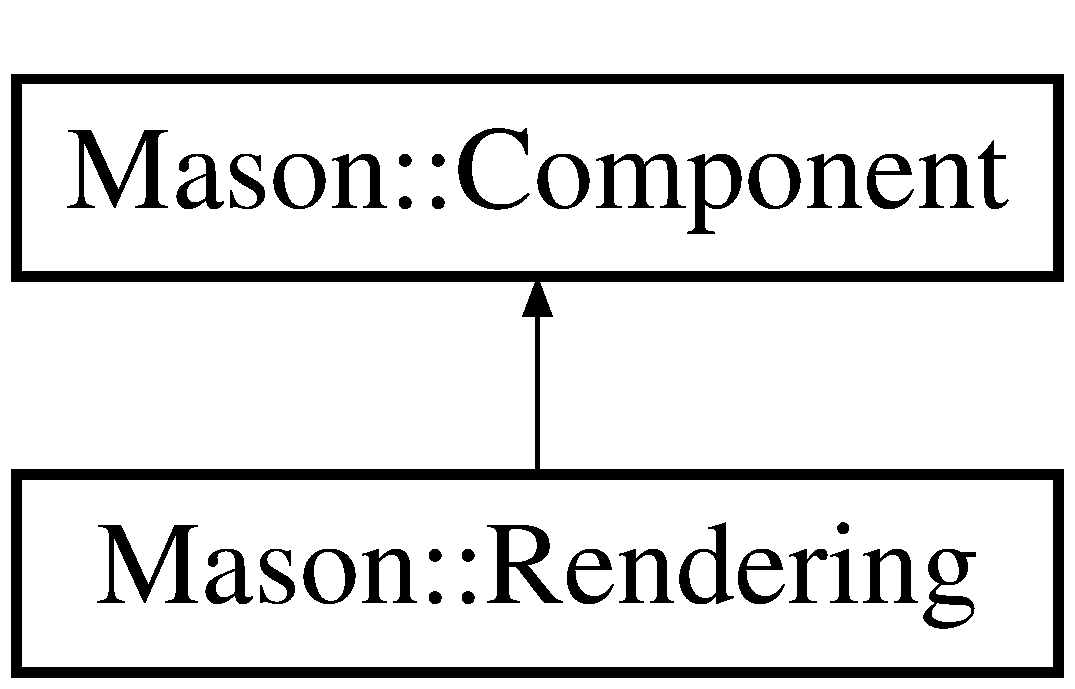
\includegraphics[height=2.000000cm]{class_mason_1_1_rendering}
\end{center}
\end{figure}
\subsection*{Public Member Functions}
\begin{DoxyCompactItemize}
\item 
void \hyperlink{class_mason_1_1_rendering_a6d279efe1ba558f425ab6bbdfa29ab48}{draw} ()
\item 
void \hyperlink{class_mason_1_1_rendering_ad27f8dd05e607f8503e0a102fa89d523}{load\+Mesh} (std\+::shared\+\_\+ptr$<$ S\+R\+E\+::\+Mesh $>$ \hyperlink{class_mason_1_1_rendering_a71855a0cbc812640516a7925be451546}{mesh})
\item 
void \hyperlink{class_mason_1_1_rendering_a3ba4b1664ba76794b6efa266fdceab6c}{load\+Shader} (std\+::shared\+\_\+ptr$<$ S\+R\+E\+::\+Shader $>$ \hyperlink{class_mason_1_1_rendering_a32477a9cf3115210280e47e9172ca407}{shader})
\item 
void \hyperlink{class_mason_1_1_rendering_aa8a7db1f0f25ac88cc6584a2a5b814ed}{set\+Color} (glm\+::vec4 \hyperlink{class_mason_1_1_rendering_a5a78c6260d5111659f1e96888a55bda1}{color})
\end{DoxyCompactItemize}
\subsection*{Protected Member Functions}
\begin{DoxyCompactItemize}
\item 
\hyperlink{class_mason_1_1_rendering_abb768ec53a7193e20f8a35d325c0a991}{Rendering} (\hyperlink{class_mason_1_1_game_object}{Game\+Object} $\ast$\hyperlink{class_mason_1_1_component_a30030370c35f5562cbbbb0927b0448c8}{game\+Object})
\end{DoxyCompactItemize}
\subsection*{Protected Attributes}
\begin{DoxyCompactItemize}
\item 
std\+::shared\+\_\+ptr$<$ S\+R\+E\+::\+Shader $>$ \hyperlink{class_mason_1_1_rendering_a32477a9cf3115210280e47e9172ca407}{shader}
\item 
std\+::shared\+\_\+ptr$<$ S\+R\+E\+::\+Mesh $>$ \hyperlink{class_mason_1_1_rendering_a71855a0cbc812640516a7925be451546}{mesh}
\item 
std\+::shared\+\_\+ptr$<$ \hyperlink{class_mason_1_1_transform}{Transform} $>$ \hyperlink{class_mason_1_1_rendering_adaca4d8bb739395f32fc4886653ed2f5}{transform}
\item 
glm\+::vec4 \hyperlink{class_mason_1_1_rendering_a5a78c6260d5111659f1e96888a55bda1}{color}
\end{DoxyCompactItemize}
\subsection*{Friends}
\begin{DoxyCompactItemize}
\item 
class \hyperlink{class_mason_1_1_rendering_a00df87c957d8f7ee0fc51f07a0542f4a}{Game\+Object}
\end{DoxyCompactItemize}


\subsection{Constructor \& Destructor Documentation}
\hypertarget{class_mason_1_1_rendering_abb768ec53a7193e20f8a35d325c0a991}{}\label{class_mason_1_1_rendering_abb768ec53a7193e20f8a35d325c0a991} 
\index{Mason\+::\+Rendering@{Mason\+::\+Rendering}!Rendering@{Rendering}}
\index{Rendering@{Rendering}!Mason\+::\+Rendering@{Mason\+::\+Rendering}}
\subsubsection{\texorpdfstring{Rendering()}{Rendering()}}
{\footnotesize\ttfamily Rendering\+::\+Rendering (\begin{DoxyParamCaption}\item[{\hyperlink{class_mason_1_1_game_object}{Game\+Object} $\ast$}]{game\+Object }\end{DoxyParamCaption})\hspace{0.3cm}{\ttfamily [protected]}}



\subsection{Member Function Documentation}
\hypertarget{class_mason_1_1_rendering_a6d279efe1ba558f425ab6bbdfa29ab48}{}\label{class_mason_1_1_rendering_a6d279efe1ba558f425ab6bbdfa29ab48} 
\index{Mason\+::\+Rendering@{Mason\+::\+Rendering}!draw@{draw}}
\index{draw@{draw}!Mason\+::\+Rendering@{Mason\+::\+Rendering}}
\subsubsection{\texorpdfstring{draw()}{draw()}}
{\footnotesize\ttfamily void Rendering\+::draw (\begin{DoxyParamCaption}{ }\end{DoxyParamCaption})}

\hypertarget{class_mason_1_1_rendering_ad27f8dd05e607f8503e0a102fa89d523}{}\label{class_mason_1_1_rendering_ad27f8dd05e607f8503e0a102fa89d523} 
\index{Mason\+::\+Rendering@{Mason\+::\+Rendering}!load\+Mesh@{load\+Mesh}}
\index{load\+Mesh@{load\+Mesh}!Mason\+::\+Rendering@{Mason\+::\+Rendering}}
\subsubsection{\texorpdfstring{load\+Mesh()}{loadMesh()}}
{\footnotesize\ttfamily void Rendering\+::load\+Mesh (\begin{DoxyParamCaption}\item[{std\+::shared\+\_\+ptr$<$ S\+R\+E\+::\+Mesh $>$}]{mesh }\end{DoxyParamCaption})}

\hypertarget{class_mason_1_1_rendering_a3ba4b1664ba76794b6efa266fdceab6c}{}\label{class_mason_1_1_rendering_a3ba4b1664ba76794b6efa266fdceab6c} 
\index{Mason\+::\+Rendering@{Mason\+::\+Rendering}!load\+Shader@{load\+Shader}}
\index{load\+Shader@{load\+Shader}!Mason\+::\+Rendering@{Mason\+::\+Rendering}}
\subsubsection{\texorpdfstring{load\+Shader()}{loadShader()}}
{\footnotesize\ttfamily void Rendering\+::load\+Shader (\begin{DoxyParamCaption}\item[{std\+::shared\+\_\+ptr$<$ S\+R\+E\+::\+Shader $>$}]{shader }\end{DoxyParamCaption})}

\hypertarget{class_mason_1_1_rendering_aa8a7db1f0f25ac88cc6584a2a5b814ed}{}\label{class_mason_1_1_rendering_aa8a7db1f0f25ac88cc6584a2a5b814ed} 
\index{Mason\+::\+Rendering@{Mason\+::\+Rendering}!set\+Color@{set\+Color}}
\index{set\+Color@{set\+Color}!Mason\+::\+Rendering@{Mason\+::\+Rendering}}
\subsubsection{\texorpdfstring{set\+Color()}{setColor()}}
{\footnotesize\ttfamily void Rendering\+::set\+Color (\begin{DoxyParamCaption}\item[{glm\+::vec4}]{color }\end{DoxyParamCaption})}



\subsection{Friends And Related Function Documentation}
\hypertarget{class_mason_1_1_rendering_a00df87c957d8f7ee0fc51f07a0542f4a}{}\label{class_mason_1_1_rendering_a00df87c957d8f7ee0fc51f07a0542f4a} 
\index{Mason\+::\+Rendering@{Mason\+::\+Rendering}!Game\+Object@{Game\+Object}}
\index{Game\+Object@{Game\+Object}!Mason\+::\+Rendering@{Mason\+::\+Rendering}}
\subsubsection{\texorpdfstring{Game\+Object}{GameObject}}
{\footnotesize\ttfamily friend class \hyperlink{class_mason_1_1_game_object}{Game\+Object}\hspace{0.3cm}{\ttfamily [friend]}}



\subsection{Member Data Documentation}
\hypertarget{class_mason_1_1_rendering_a5a78c6260d5111659f1e96888a55bda1}{}\label{class_mason_1_1_rendering_a5a78c6260d5111659f1e96888a55bda1} 
\index{Mason\+::\+Rendering@{Mason\+::\+Rendering}!color@{color}}
\index{color@{color}!Mason\+::\+Rendering@{Mason\+::\+Rendering}}
\subsubsection{\texorpdfstring{color}{color}}
{\footnotesize\ttfamily glm\+::vec4 Mason\+::\+Rendering\+::color\hspace{0.3cm}{\ttfamily [protected]}}

\hypertarget{class_mason_1_1_rendering_a71855a0cbc812640516a7925be451546}{}\label{class_mason_1_1_rendering_a71855a0cbc812640516a7925be451546} 
\index{Mason\+::\+Rendering@{Mason\+::\+Rendering}!mesh@{mesh}}
\index{mesh@{mesh}!Mason\+::\+Rendering@{Mason\+::\+Rendering}}
\subsubsection{\texorpdfstring{mesh}{mesh}}
{\footnotesize\ttfamily std\+::shared\+\_\+ptr$<$S\+R\+E\+::\+Mesh$>$ Mason\+::\+Rendering\+::mesh\hspace{0.3cm}{\ttfamily [protected]}}

\hypertarget{class_mason_1_1_rendering_a32477a9cf3115210280e47e9172ca407}{}\label{class_mason_1_1_rendering_a32477a9cf3115210280e47e9172ca407} 
\index{Mason\+::\+Rendering@{Mason\+::\+Rendering}!shader@{shader}}
\index{shader@{shader}!Mason\+::\+Rendering@{Mason\+::\+Rendering}}
\subsubsection{\texorpdfstring{shader}{shader}}
{\footnotesize\ttfamily std\+::shared\+\_\+ptr$<$S\+R\+E\+::\+Shader$>$ Mason\+::\+Rendering\+::shader\hspace{0.3cm}{\ttfamily [protected]}}

\hypertarget{class_mason_1_1_rendering_adaca4d8bb739395f32fc4886653ed2f5}{}\label{class_mason_1_1_rendering_adaca4d8bb739395f32fc4886653ed2f5} 
\index{Mason\+::\+Rendering@{Mason\+::\+Rendering}!transform@{transform}}
\index{transform@{transform}!Mason\+::\+Rendering@{Mason\+::\+Rendering}}
\subsubsection{\texorpdfstring{transform}{transform}}
{\footnotesize\ttfamily std\+::shared\+\_\+ptr$<$\hyperlink{class_mason_1_1_transform}{Transform}$>$ Mason\+::\+Rendering\+::transform\hspace{0.3cm}{\ttfamily [protected]}}



The documentation for this class was generated from the following files\+:\begin{DoxyCompactItemize}
\item 
C\+:/\+Users/\+Carol/\+Documents/\+Git\+Hub/\+Team\+Does\+Not\+Matter/\+Engine/include/\+Mason/\hyperlink{_rendering_8h}{Rendering.\+h}\item 
C\+:/\+Users/\+Carol/\+Documents/\+Git\+Hub/\+Team\+Does\+Not\+Matter/\+Engine/src/\hyperlink{_rendering_8cpp}{Rendering.\+cpp}\end{DoxyCompactItemize}

\hypertarget{class_mason_1_1_scene}{}\section{Mason\+:\+:Scene Class Reference}
\label{class_mason_1_1_scene}\index{Mason\+::\+Scene@{Mason\+::\+Scene}}


{\ttfamily \#include $<$Scene.\+hpp$>$}

\subsection*{Public Member Functions}
\begin{DoxyCompactItemize}
\item 
\hyperlink{class_mason_1_1_scene_ad10176d75a9cc0da56626f682d083507}{Scene} ()
\begin{DoxyCompactList}\small\item\em constructor \end{DoxyCompactList}\item 
std\+::shared\+\_\+ptr$<$ \hyperlink{class_mason_1_1_game_object}{Game\+Object} $>$ \hyperlink{class_mason_1_1_scene_afe8ac9cb371c04a0587faf06bf828ac9}{add\+Game\+Object} (std\+::string name)
\begin{DoxyCompactList}\small\item\em Add game object. \end{DoxyCompactList}\item 
std\+::shared\+\_\+ptr$<$ \hyperlink{class_mason_1_1_game_object}{Game\+Object} $>$ \hyperlink{class_mason_1_1_scene_a4d1afc4d112079aedd3829a8a42e902e}{load\+Game\+Object} (\hyperlink{class_mason_1_1_game_object_descriptor}{Game\+Object\+Descriptor} desc)
\begin{DoxyCompactList}\small\item\em Load game object from decriptor. \end{DoxyCompactList}\item 
void \hyperlink{class_mason_1_1_scene_a2d10aca9d364dc70935795a1436f353d}{set\+Parent\+Relationship} (int child\+Id, int parent\+Id)
\begin{DoxyCompactList}\small\item\em Setup a parent-\/child relationship between gameobjects. \end{DoxyCompactList}\item 
bool \hyperlink{class_mason_1_1_scene_aad5427fcdd330f65dc4e7b1e627afce4}{remove\+Game\+Object} (std\+::shared\+\_\+ptr$<$ \hyperlink{class_mason_1_1_game_object}{Game\+Object} $>$ ptr)
\begin{DoxyCompactList}\small\item\em Remove game object. \end{DoxyCompactList}\item 
int \hyperlink{class_mason_1_1_scene_a97780dbb825e92c62b02623fe1e297fa}{get\+Size} ()
\begin{DoxyCompactList}\small\item\em Get number of game objects. \end{DoxyCompactList}\item 
std\+::shared\+\_\+ptr$<$ \hyperlink{class_mason_1_1_game_object}{Game\+Object} $>$ \hyperlink{class_mason_1_1_scene_ae13738888d4f00135fb827639f87239b}{get\+Game\+Object} (int index)
\begin{DoxyCompactList}\small\item\em Get game object by index. \end{DoxyCompactList}\item 
std\+::vector$<$ std\+::shared\+\_\+ptr$<$ \hyperlink{class_mason_1_1_game_object}{Game\+Object} $>$ $>$ \hyperlink{class_mason_1_1_scene_a045d786fa6f11ab01e190971637b15ce}{get\+Game\+Objects} ()
\begin{DoxyCompactList}\small\item\em Get all game objects. \end{DoxyCompactList}\item 
{\footnotesize template$<$typename C $>$ }\\std\+::vector$<$ C $\ast$ $>$ \hyperlink{class_mason_1_1_scene_a889caa86c1c4c8fad9416c7240148232}{get\+All\+Component} ()
\begin{DoxyCompactList}\small\item\em Returns all components of type C. \end{DoxyCompactList}\end{DoxyCompactItemize}
\subsection*{Static Public Member Functions}
\begin{DoxyCompactItemize}
\item 
static std\+::shared\+\_\+ptr$<$ \hyperlink{class_mason_1_1_game_object}{Game\+Object} $>$ \hyperlink{class_mason_1_1_scene_a3eee172075ff2b845caffc8e641f9d9c}{Instantiate} (std\+::string name)
\item 
static void \hyperlink{class_mason_1_1_scene_a4721fcf8438883759478aee25bf247c2}{Destroy} (std\+::shared\+\_\+ptr$<$ \hyperlink{class_mason_1_1_game_object}{Game\+Object} $>$ ptr)
\item 
static void \hyperlink{class_mason_1_1_scene_a8f395f22c024c0d5161cfa8e024f177d}{Destroy} (\hyperlink{class_mason_1_1_game_object}{Game\+Object} $\ast$ptr)
\item 
static std\+::vector$<$ std\+::shared\+\_\+ptr$<$ \hyperlink{class_mason_1_1_game_object}{Game\+Object} $>$ $>$ \hyperlink{class_mason_1_1_scene_a684a224fe56794d0db86da99947a6fac}{Get\+By\+Name} (std\+::string name)
\end{DoxyCompactItemize}
\subsection*{Friends}
\begin{DoxyCompactItemize}
\item 
class \hyperlink{class_mason_1_1_scene_a3e1914489e4bed4f9f23cdeab34a43dc}{Engine}
\end{DoxyCompactItemize}


\subsection{Detailed Description}
Game\+Objects, sprites, paths to images, templates, and sounds 

\subsection{Constructor \& Destructor Documentation}
\hypertarget{class_mason_1_1_scene_ad10176d75a9cc0da56626f682d083507}{}\label{class_mason_1_1_scene_ad10176d75a9cc0da56626f682d083507} 
\index{Mason\+::\+Scene@{Mason\+::\+Scene}!Scene@{Scene}}
\index{Scene@{Scene}!Mason\+::\+Scene@{Mason\+::\+Scene}}
\subsubsection{\texorpdfstring{Scene()}{Scene()}}
{\footnotesize\ttfamily Scene\+::\+Scene (\begin{DoxyParamCaption}{ }\end{DoxyParamCaption})}



constructor 



\subsection{Member Function Documentation}
\hypertarget{class_mason_1_1_scene_afe8ac9cb371c04a0587faf06bf828ac9}{}\label{class_mason_1_1_scene_afe8ac9cb371c04a0587faf06bf828ac9} 
\index{Mason\+::\+Scene@{Mason\+::\+Scene}!add\+Game\+Object@{add\+Game\+Object}}
\index{add\+Game\+Object@{add\+Game\+Object}!Mason\+::\+Scene@{Mason\+::\+Scene}}
\subsubsection{\texorpdfstring{add\+Game\+Object()}{addGameObject()}}
{\footnotesize\ttfamily shared\+\_\+ptr$<$ \hyperlink{class_mason_1_1_game_object}{Game\+Object} $>$ Scene\+::add\+Game\+Object (\begin{DoxyParamCaption}\item[{std\+::string}]{name }\end{DoxyParamCaption})}



Add game object. 

\hypertarget{class_mason_1_1_scene_a4721fcf8438883759478aee25bf247c2}{}\label{class_mason_1_1_scene_a4721fcf8438883759478aee25bf247c2} 
\index{Mason\+::\+Scene@{Mason\+::\+Scene}!Destroy@{Destroy}}
\index{Destroy@{Destroy}!Mason\+::\+Scene@{Mason\+::\+Scene}}
\subsubsection{\texorpdfstring{Destroy()}{Destroy()}\hspace{0.1cm}{\footnotesize\ttfamily [1/2]}}
{\footnotesize\ttfamily static void Mason\+::\+Scene\+::\+Destroy (\begin{DoxyParamCaption}\item[{std\+::shared\+\_\+ptr$<$ \hyperlink{class_mason_1_1_game_object}{Game\+Object} $>$}]{ptr }\end{DoxyParamCaption})\hspace{0.3cm}{\ttfamily [static]}}

\hypertarget{class_mason_1_1_scene_a8f395f22c024c0d5161cfa8e024f177d}{}\label{class_mason_1_1_scene_a8f395f22c024c0d5161cfa8e024f177d} 
\index{Mason\+::\+Scene@{Mason\+::\+Scene}!Destroy@{Destroy}}
\index{Destroy@{Destroy}!Mason\+::\+Scene@{Mason\+::\+Scene}}
\subsubsection{\texorpdfstring{Destroy()}{Destroy()}\hspace{0.1cm}{\footnotesize\ttfamily [2/2]}}
{\footnotesize\ttfamily void Scene\+::\+Destroy (\begin{DoxyParamCaption}\item[{\hyperlink{class_mason_1_1_game_object}{Game\+Object} $\ast$}]{ptr }\end{DoxyParamCaption})\hspace{0.3cm}{\ttfamily [static]}}

\hypertarget{class_mason_1_1_scene_a889caa86c1c4c8fad9416c7240148232}{}\label{class_mason_1_1_scene_a889caa86c1c4c8fad9416c7240148232} 
\index{Mason\+::\+Scene@{Mason\+::\+Scene}!get\+All\+Component@{get\+All\+Component}}
\index{get\+All\+Component@{get\+All\+Component}!Mason\+::\+Scene@{Mason\+::\+Scene}}
\subsubsection{\texorpdfstring{get\+All\+Component()}{getAllComponent()}}
{\footnotesize\ttfamily template$<$typename C $>$ \\
std\+::vector$<$ C $\ast$ $>$ Mason\+::\+Scene\+::get\+All\+Component (\begin{DoxyParamCaption}{ }\end{DoxyParamCaption})}



Returns all components of type C. 

gets all the components of the scene

\begin{DoxyReturn}{Returns}
std\+::vector$<$\+C$\ast$$>$ 
\end{DoxyReturn}
\hypertarget{class_mason_1_1_scene_a684a224fe56794d0db86da99947a6fac}{}\label{class_mason_1_1_scene_a684a224fe56794d0db86da99947a6fac} 
\index{Mason\+::\+Scene@{Mason\+::\+Scene}!Get\+By\+Name@{Get\+By\+Name}}
\index{Get\+By\+Name@{Get\+By\+Name}!Mason\+::\+Scene@{Mason\+::\+Scene}}
\subsubsection{\texorpdfstring{Get\+By\+Name()}{GetByName()}}
{\footnotesize\ttfamily vector$<$ shared\+\_\+ptr$<$ \hyperlink{class_mason_1_1_game_object}{Game\+Object} $>$ $>$ Scene\+::\+Get\+By\+Name (\begin{DoxyParamCaption}\item[{std\+::string}]{name }\end{DoxyParamCaption})\hspace{0.3cm}{\ttfamily [static]}}

\hypertarget{class_mason_1_1_scene_ae13738888d4f00135fb827639f87239b}{}\label{class_mason_1_1_scene_ae13738888d4f00135fb827639f87239b} 
\index{Mason\+::\+Scene@{Mason\+::\+Scene}!get\+Game\+Object@{get\+Game\+Object}}
\index{get\+Game\+Object@{get\+Game\+Object}!Mason\+::\+Scene@{Mason\+::\+Scene}}
\subsubsection{\texorpdfstring{get\+Game\+Object()}{getGameObject()}}
{\footnotesize\ttfamily shared\+\_\+ptr$<$ \hyperlink{class_mason_1_1_game_object}{Game\+Object} $>$ Scene\+::get\+Game\+Object (\begin{DoxyParamCaption}\item[{int}]{index }\end{DoxyParamCaption})}



Get game object by index. 

\hypertarget{class_mason_1_1_scene_a045d786fa6f11ab01e190971637b15ce}{}\label{class_mason_1_1_scene_a045d786fa6f11ab01e190971637b15ce} 
\index{Mason\+::\+Scene@{Mason\+::\+Scene}!get\+Game\+Objects@{get\+Game\+Objects}}
\index{get\+Game\+Objects@{get\+Game\+Objects}!Mason\+::\+Scene@{Mason\+::\+Scene}}
\subsubsection{\texorpdfstring{get\+Game\+Objects()}{getGameObjects()}}
{\footnotesize\ttfamily vector$<$ shared\+\_\+ptr$<$ \hyperlink{class_mason_1_1_game_object}{Game\+Object} $>$ $>$ Scene\+::get\+Game\+Objects (\begin{DoxyParamCaption}{ }\end{DoxyParamCaption})}



Get all game objects. 

\hypertarget{class_mason_1_1_scene_a97780dbb825e92c62b02623fe1e297fa}{}\label{class_mason_1_1_scene_a97780dbb825e92c62b02623fe1e297fa} 
\index{Mason\+::\+Scene@{Mason\+::\+Scene}!get\+Size@{get\+Size}}
\index{get\+Size@{get\+Size}!Mason\+::\+Scene@{Mason\+::\+Scene}}
\subsubsection{\texorpdfstring{get\+Size()}{getSize()}}
{\footnotesize\ttfamily int Scene\+::get\+Size (\begin{DoxyParamCaption}{ }\end{DoxyParamCaption})}



Get number of game objects. 

\hypertarget{class_mason_1_1_scene_a3eee172075ff2b845caffc8e641f9d9c}{}\label{class_mason_1_1_scene_a3eee172075ff2b845caffc8e641f9d9c} 
\index{Mason\+::\+Scene@{Mason\+::\+Scene}!Instantiate@{Instantiate}}
\index{Instantiate@{Instantiate}!Mason\+::\+Scene@{Mason\+::\+Scene}}
\subsubsection{\texorpdfstring{Instantiate()}{Instantiate()}}
{\footnotesize\ttfamily shared\+\_\+ptr$<$ \hyperlink{class_mason_1_1_game_object}{Game\+Object} $>$ Scene\+::\+Instantiate (\begin{DoxyParamCaption}\item[{std\+::string}]{name }\end{DoxyParamCaption})\hspace{0.3cm}{\ttfamily [static]}}

\hypertarget{class_mason_1_1_scene_a4d1afc4d112079aedd3829a8a42e902e}{}\label{class_mason_1_1_scene_a4d1afc4d112079aedd3829a8a42e902e} 
\index{Mason\+::\+Scene@{Mason\+::\+Scene}!load\+Game\+Object@{load\+Game\+Object}}
\index{load\+Game\+Object@{load\+Game\+Object}!Mason\+::\+Scene@{Mason\+::\+Scene}}
\subsubsection{\texorpdfstring{load\+Game\+Object()}{loadGameObject()}}
{\footnotesize\ttfamily shared\+\_\+ptr$<$ \hyperlink{class_mason_1_1_game_object}{Game\+Object} $>$ Scene\+::load\+Game\+Object (\begin{DoxyParamCaption}\item[{\hyperlink{class_mason_1_1_game_object_descriptor}{Game\+Object\+Descriptor}}]{desc }\end{DoxyParamCaption})}



Load game object from decriptor. 

\hypertarget{class_mason_1_1_scene_aad5427fcdd330f65dc4e7b1e627afce4}{}\label{class_mason_1_1_scene_aad5427fcdd330f65dc4e7b1e627afce4} 
\index{Mason\+::\+Scene@{Mason\+::\+Scene}!remove\+Game\+Object@{remove\+Game\+Object}}
\index{remove\+Game\+Object@{remove\+Game\+Object}!Mason\+::\+Scene@{Mason\+::\+Scene}}
\subsubsection{\texorpdfstring{remove\+Game\+Object()}{removeGameObject()}}
{\footnotesize\ttfamily bool Scene\+::remove\+Game\+Object (\begin{DoxyParamCaption}\item[{std\+::shared\+\_\+ptr$<$ \hyperlink{class_mason_1_1_game_object}{Game\+Object} $>$}]{ptr }\end{DoxyParamCaption})}



Remove game object. 

\hypertarget{class_mason_1_1_scene_a2d10aca9d364dc70935795a1436f353d}{}\label{class_mason_1_1_scene_a2d10aca9d364dc70935795a1436f353d} 
\index{Mason\+::\+Scene@{Mason\+::\+Scene}!set\+Parent\+Relationship@{set\+Parent\+Relationship}}
\index{set\+Parent\+Relationship@{set\+Parent\+Relationship}!Mason\+::\+Scene@{Mason\+::\+Scene}}
\subsubsection{\texorpdfstring{set\+Parent\+Relationship()}{setParentRelationship()}}
{\footnotesize\ttfamily void Scene\+::set\+Parent\+Relationship (\begin{DoxyParamCaption}\item[{int}]{child\+Id,  }\item[{int}]{parent\+Id }\end{DoxyParamCaption})}



Setup a parent-\/child relationship between gameobjects. 



\subsection{Friends And Related Function Documentation}
\hypertarget{class_mason_1_1_scene_a3e1914489e4bed4f9f23cdeab34a43dc}{}\label{class_mason_1_1_scene_a3e1914489e4bed4f9f23cdeab34a43dc} 
\index{Mason\+::\+Scene@{Mason\+::\+Scene}!Engine@{Engine}}
\index{Engine@{Engine}!Mason\+::\+Scene@{Mason\+::\+Scene}}
\subsubsection{\texorpdfstring{Engine}{Engine}}
{\footnotesize\ttfamily friend class \hyperlink{class_mason_1_1_engine}{Engine}\hspace{0.3cm}{\ttfamily [friend]}}



The documentation for this class was generated from the following files\+:\begin{DoxyCompactItemize}
\item 
include/\+Mason/\hyperlink{_scene_8hpp}{Scene.\+hpp}\item 
src/\hyperlink{_scene_8cpp}{Scene.\+cpp}\end{DoxyCompactItemize}

\hypertarget{class_mason_1_1_scene_parser}{}\section{Mason\+:\+:Scene\+Parser Class Reference}
\label{class_mason_1_1_scene_parser}\index{Mason\+::\+Scene\+Parser@{Mason\+::\+Scene\+Parser}}


{\ttfamily \#include $<$Scene\+Parser.\+hpp$>$}

\subsection*{Static Public Member Functions}
\begin{DoxyCompactItemize}
\item 
static std\+::vector$<$ \hyperlink{class_mason_1_1_game_object_descriptor}{Game\+Object\+Descriptor} $>$ \hyperlink{class_mason_1_1_scene_parser_a3f69f475dee046264762e618e70b78e6}{parse\+File} (std\+::string filename)
\end{DoxyCompactItemize}


\subsection{Member Function Documentation}
\hypertarget{class_mason_1_1_scene_parser_a3f69f475dee046264762e618e70b78e6}{}\label{class_mason_1_1_scene_parser_a3f69f475dee046264762e618e70b78e6} 
\index{Mason\+::\+Scene\+Parser@{Mason\+::\+Scene\+Parser}!parse\+File@{parse\+File}}
\index{parse\+File@{parse\+File}!Mason\+::\+Scene\+Parser@{Mason\+::\+Scene\+Parser}}
\subsubsection{\texorpdfstring{parse\+File()}{parseFile()}}
{\footnotesize\ttfamily std\+::vector$<$ \hyperlink{class_mason_1_1_game_object_descriptor}{Game\+Object\+Descriptor} $>$ Scene\+Parser\+::parse\+File (\begin{DoxyParamCaption}\item[{std\+::string}]{filename }\end{DoxyParamCaption})\hspace{0.3cm}{\ttfamily [static]}}



The documentation for this class was generated from the following files\+:\begin{DoxyCompactItemize}
\item 
C\+:/\+Users/\+Carol/\+Documents/\+Git\+Hub/\+Team\+Does\+Not\+Matter/\+Engine/include/\+Mason/\hyperlink{_scene_parser_8hpp}{Scene\+Parser.\+hpp}\item 
C\+:/\+Users/\+Carol/\+Documents/\+Git\+Hub/\+Team\+Does\+Not\+Matter/\+Engine/src/\hyperlink{_scene_parser_8cpp}{Scene\+Parser.\+cpp}\end{DoxyCompactItemize}

\hypertarget{class_mason_1_1_script}{}\section{Mason\+:\+:Script Class Reference}
\label{class_mason_1_1_script}\index{Mason\+::\+Script@{Mason\+::\+Script}}


{\ttfamily \#include $<$Script.\+hpp$>$}

Inheritance diagram for Mason\+:\+:Script\+:\begin{figure}[H]
\begin{center}
\leavevmode
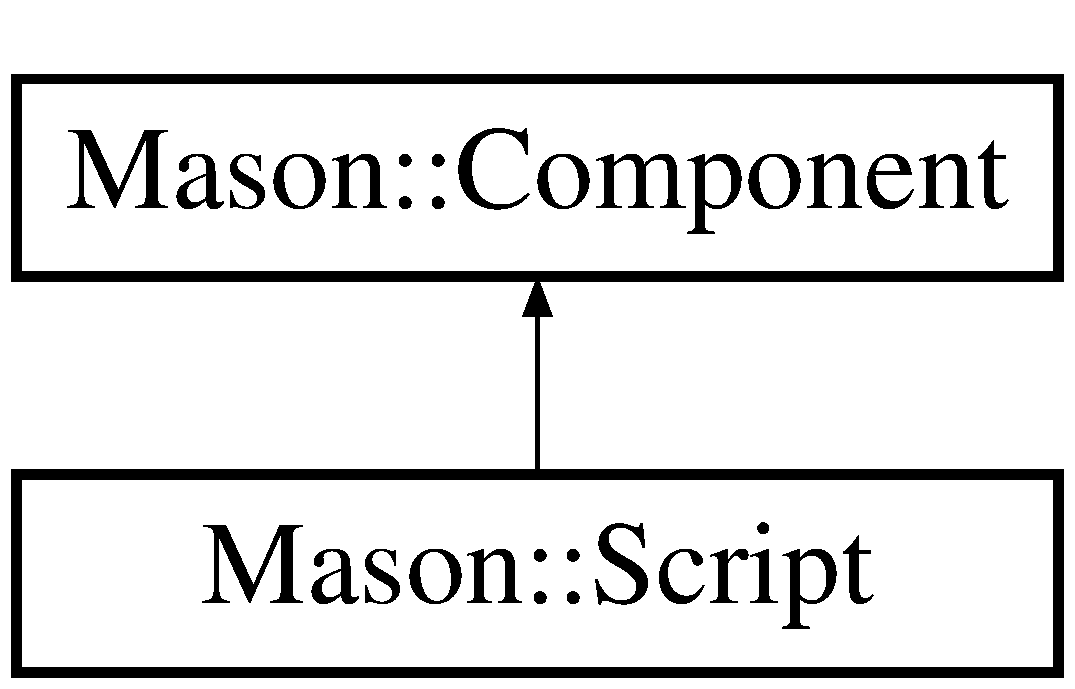
\includegraphics[height=2.000000cm]{class_mason_1_1_script}
\end{center}
\end{figure}
\subsection*{Public Member Functions}
\begin{DoxyCompactItemize}
\item 
\hyperlink{class_mason_1_1_script_a3d41c440d07b53c15437a13754eff7d0}{Script} (std\+::shared\+\_\+ptr$<$ \hyperlink{class_mason_1_1_game_object}{Game\+Object} $>$ \hyperlink{class_mason_1_1_component_abaa67b569d0a70e26a4606f4a099a925}{game\+Object})
\item 
virtual void \hyperlink{class_mason_1_1_script_aa42915c752bb7f4623ca679b222edf2f}{On\+Start} ()
\item 
virtual void \hyperlink{class_mason_1_1_script_acafa4283460fb677484bb43ebec37743}{On\+Update} ()
\item 
virtual void \hyperlink{class_mason_1_1_script_a1088013d6edc47d74643aa48a7cbbbdf}{On\+Collision\+Enter} (\hyperlink{class_mason_1_1_game_object}{Game\+Object} $\ast$other)
\item 
virtual void \hyperlink{class_mason_1_1_script_a04d09648b7dba1bcb0a0ad3c3570e2f3}{On\+Collision\+Exit} (\hyperlink{class_mason_1_1_game_object}{Game\+Object} $\ast$other)
\item 
virtual void \hyperlink{class_mason_1_1_script_a84fff8072c4e8b56fb242b29f3491224}{On\+Input} (S\+D\+L\+\_\+\+Event event)
\item 
virtual void \hyperlink{class_mason_1_1_script_aa993a4ef5572ba31f5fa0ce2fa4a733e}{On\+G\+UI} ()
\end{DoxyCompactItemize}
\subsection*{Public Attributes}
\begin{DoxyCompactItemize}
\item 
std\+::shared\+\_\+ptr$<$ \hyperlink{class_mason_1_1_game_object}{Game\+Object} $>$ \hyperlink{class_mason_1_1_script_a26ffab9ad2a0f22cb6a3cba3029a985f}{gameobject}
\item 
\hyperlink{class_mason_1_1_transform}{Transform} $\ast$ \hyperlink{class_mason_1_1_script_a4ac6ab2299555435468ba62c52ede167}{transform}
\item 
std\+::map$<$ std\+::string, std\+::string $>$ \hyperlink{class_mason_1_1_script_a96f691d0ccd8db2e3e95824e8579cc42}{strings}
\item 
std\+::map$<$ std\+::string, float $>$ \hyperlink{class_mason_1_1_script_a39ec15b6842f815f09537f524c0b0786}{numbers}
\end{DoxyCompactItemize}
\subsection*{Static Public Attributes}
\begin{DoxyCompactItemize}
\item 
static std\+::map$<$ std\+::string, \hyperlink{class_mason_1_1_script}{Script} $\ast$($\ast$)(std\+::shared\+\_\+ptr$<$ \hyperlink{class_mason_1_1_game_object}{Game\+Object} $>$)$>$ \hyperlink{class_mason_1_1_script_a0b74a1b2b601b05841c95b44b329f859}{scripts} = std\+::map$<$std\+::string, \hyperlink{class_mason_1_1_script}{Script}$\ast$($\ast$)(std\+::shared\+\_\+ptr$<$\hyperlink{class_mason_1_1_game_object}{Game\+Object}$>$)$>$()
\end{DoxyCompactItemize}
\subsection*{Friends}
\begin{DoxyCompactItemize}
\item 
class \hyperlink{class_mason_1_1_script_a3e1914489e4bed4f9f23cdeab34a43dc}{Engine}
\end{DoxyCompactItemize}
\subsection*{Additional Inherited Members}


\subsection{Constructor \& Destructor Documentation}
\hypertarget{class_mason_1_1_script_a3d41c440d07b53c15437a13754eff7d0}{}\label{class_mason_1_1_script_a3d41c440d07b53c15437a13754eff7d0} 
\index{Mason\+::\+Script@{Mason\+::\+Script}!Script@{Script}}
\index{Script@{Script}!Mason\+::\+Script@{Mason\+::\+Script}}
\subsubsection{\texorpdfstring{Script()}{Script()}}
{\footnotesize\ttfamily Mason\+::\+Script\+::\+Script (\begin{DoxyParamCaption}\item[{std\+::shared\+\_\+ptr$<$ \hyperlink{class_mason_1_1_game_object}{Game\+Object} $>$}]{game\+Object }\end{DoxyParamCaption})\hspace{0.3cm}{\ttfamily [inline]}}



\subsection{Member Function Documentation}
\hypertarget{class_mason_1_1_script_a1088013d6edc47d74643aa48a7cbbbdf}{}\label{class_mason_1_1_script_a1088013d6edc47d74643aa48a7cbbbdf} 
\index{Mason\+::\+Script@{Mason\+::\+Script}!On\+Collision\+Enter@{On\+Collision\+Enter}}
\index{On\+Collision\+Enter@{On\+Collision\+Enter}!Mason\+::\+Script@{Mason\+::\+Script}}
\subsubsection{\texorpdfstring{On\+Collision\+Enter()}{OnCollisionEnter()}}
{\footnotesize\ttfamily virtual void Mason\+::\+Script\+::\+On\+Collision\+Enter (\begin{DoxyParamCaption}\item[{\hyperlink{class_mason_1_1_game_object}{Game\+Object} $\ast$}]{other }\end{DoxyParamCaption})\hspace{0.3cm}{\ttfamily [inline]}, {\ttfamily [virtual]}}

\hypertarget{class_mason_1_1_script_a04d09648b7dba1bcb0a0ad3c3570e2f3}{}\label{class_mason_1_1_script_a04d09648b7dba1bcb0a0ad3c3570e2f3} 
\index{Mason\+::\+Script@{Mason\+::\+Script}!On\+Collision\+Exit@{On\+Collision\+Exit}}
\index{On\+Collision\+Exit@{On\+Collision\+Exit}!Mason\+::\+Script@{Mason\+::\+Script}}
\subsubsection{\texorpdfstring{On\+Collision\+Exit()}{OnCollisionExit()}}
{\footnotesize\ttfamily virtual void Mason\+::\+Script\+::\+On\+Collision\+Exit (\begin{DoxyParamCaption}\item[{\hyperlink{class_mason_1_1_game_object}{Game\+Object} $\ast$}]{other }\end{DoxyParamCaption})\hspace{0.3cm}{\ttfamily [inline]}, {\ttfamily [virtual]}}

\hypertarget{class_mason_1_1_script_aa993a4ef5572ba31f5fa0ce2fa4a733e}{}\label{class_mason_1_1_script_aa993a4ef5572ba31f5fa0ce2fa4a733e} 
\index{Mason\+::\+Script@{Mason\+::\+Script}!On\+G\+UI@{On\+G\+UI}}
\index{On\+G\+UI@{On\+G\+UI}!Mason\+::\+Script@{Mason\+::\+Script}}
\subsubsection{\texorpdfstring{On\+G\+U\+I()}{OnGUI()}}
{\footnotesize\ttfamily virtual void Mason\+::\+Script\+::\+On\+G\+UI (\begin{DoxyParamCaption}{ }\end{DoxyParamCaption})\hspace{0.3cm}{\ttfamily [inline]}, {\ttfamily [virtual]}}

\hypertarget{class_mason_1_1_script_a84fff8072c4e8b56fb242b29f3491224}{}\label{class_mason_1_1_script_a84fff8072c4e8b56fb242b29f3491224} 
\index{Mason\+::\+Script@{Mason\+::\+Script}!On\+Input@{On\+Input}}
\index{On\+Input@{On\+Input}!Mason\+::\+Script@{Mason\+::\+Script}}
\subsubsection{\texorpdfstring{On\+Input()}{OnInput()}}
{\footnotesize\ttfamily virtual void Mason\+::\+Script\+::\+On\+Input (\begin{DoxyParamCaption}\item[{S\+D\+L\+\_\+\+Event}]{event }\end{DoxyParamCaption})\hspace{0.3cm}{\ttfamily [inline]}, {\ttfamily [virtual]}}

\hypertarget{class_mason_1_1_script_aa42915c752bb7f4623ca679b222edf2f}{}\label{class_mason_1_1_script_aa42915c752bb7f4623ca679b222edf2f} 
\index{Mason\+::\+Script@{Mason\+::\+Script}!On\+Start@{On\+Start}}
\index{On\+Start@{On\+Start}!Mason\+::\+Script@{Mason\+::\+Script}}
\subsubsection{\texorpdfstring{On\+Start()}{OnStart()}}
{\footnotesize\ttfamily virtual void Mason\+::\+Script\+::\+On\+Start (\begin{DoxyParamCaption}{ }\end{DoxyParamCaption})\hspace{0.3cm}{\ttfamily [inline]}, {\ttfamily [virtual]}}

\hypertarget{class_mason_1_1_script_acafa4283460fb677484bb43ebec37743}{}\label{class_mason_1_1_script_acafa4283460fb677484bb43ebec37743} 
\index{Mason\+::\+Script@{Mason\+::\+Script}!On\+Update@{On\+Update}}
\index{On\+Update@{On\+Update}!Mason\+::\+Script@{Mason\+::\+Script}}
\subsubsection{\texorpdfstring{On\+Update()}{OnUpdate()}}
{\footnotesize\ttfamily virtual void Mason\+::\+Script\+::\+On\+Update (\begin{DoxyParamCaption}{ }\end{DoxyParamCaption})\hspace{0.3cm}{\ttfamily [inline]}, {\ttfamily [virtual]}}



\subsection{Friends And Related Function Documentation}
\hypertarget{class_mason_1_1_script_a3e1914489e4bed4f9f23cdeab34a43dc}{}\label{class_mason_1_1_script_a3e1914489e4bed4f9f23cdeab34a43dc} 
\index{Mason\+::\+Script@{Mason\+::\+Script}!Engine@{Engine}}
\index{Engine@{Engine}!Mason\+::\+Script@{Mason\+::\+Script}}
\subsubsection{\texorpdfstring{Engine}{Engine}}
{\footnotesize\ttfamily friend class \hyperlink{class_mason_1_1_engine}{Engine}\hspace{0.3cm}{\ttfamily [friend]}}



\subsection{Member Data Documentation}
\hypertarget{class_mason_1_1_script_a26ffab9ad2a0f22cb6a3cba3029a985f}{}\label{class_mason_1_1_script_a26ffab9ad2a0f22cb6a3cba3029a985f} 
\index{Mason\+::\+Script@{Mason\+::\+Script}!gameobject@{gameobject}}
\index{gameobject@{gameobject}!Mason\+::\+Script@{Mason\+::\+Script}}
\subsubsection{\texorpdfstring{gameobject}{gameobject}}
{\footnotesize\ttfamily std\+::shared\+\_\+ptr$<$\hyperlink{class_mason_1_1_game_object}{Game\+Object}$>$ Mason\+::\+Script\+::gameobject}

\hypertarget{class_mason_1_1_script_a39ec15b6842f815f09537f524c0b0786}{}\label{class_mason_1_1_script_a39ec15b6842f815f09537f524c0b0786} 
\index{Mason\+::\+Script@{Mason\+::\+Script}!numbers@{numbers}}
\index{numbers@{numbers}!Mason\+::\+Script@{Mason\+::\+Script}}
\subsubsection{\texorpdfstring{numbers}{numbers}}
{\footnotesize\ttfamily std\+::map$<$std\+::string, float$>$ Mason\+::\+Script\+::numbers}

\hypertarget{class_mason_1_1_script_a0b74a1b2b601b05841c95b44b329f859}{}\label{class_mason_1_1_script_a0b74a1b2b601b05841c95b44b329f859} 
\index{Mason\+::\+Script@{Mason\+::\+Script}!scripts@{scripts}}
\index{scripts@{scripts}!Mason\+::\+Script@{Mason\+::\+Script}}
\subsubsection{\texorpdfstring{scripts}{scripts}}
{\footnotesize\ttfamily std\+::map$<$ std\+::string, \hyperlink{class_mason_1_1_script}{Script} $\ast$($\ast$)(std\+::shared\+\_\+ptr$<$ \hyperlink{class_mason_1_1_game_object}{Game\+Object} $>$)$>$ Script\+::scripts = std\+::map$<$std\+::string, \hyperlink{class_mason_1_1_script}{Script}$\ast$($\ast$)(std\+::shared\+\_\+ptr$<$\hyperlink{class_mason_1_1_game_object}{Game\+Object}$>$)$>$()\hspace{0.3cm}{\ttfamily [static]}}

\hypertarget{class_mason_1_1_script_a96f691d0ccd8db2e3e95824e8579cc42}{}\label{class_mason_1_1_script_a96f691d0ccd8db2e3e95824e8579cc42} 
\index{Mason\+::\+Script@{Mason\+::\+Script}!strings@{strings}}
\index{strings@{strings}!Mason\+::\+Script@{Mason\+::\+Script}}
\subsubsection{\texorpdfstring{strings}{strings}}
{\footnotesize\ttfamily std\+::map$<$std\+::string, std\+::string$>$ Mason\+::\+Script\+::strings}

\hypertarget{class_mason_1_1_script_a4ac6ab2299555435468ba62c52ede167}{}\label{class_mason_1_1_script_a4ac6ab2299555435468ba62c52ede167} 
\index{Mason\+::\+Script@{Mason\+::\+Script}!transform@{transform}}
\index{transform@{transform}!Mason\+::\+Script@{Mason\+::\+Script}}
\subsubsection{\texorpdfstring{transform}{transform}}
{\footnotesize\ttfamily \hyperlink{class_mason_1_1_transform}{Transform}$\ast$ Mason\+::\+Script\+::transform}



The documentation for this class was generated from the following files\+:\begin{DoxyCompactItemize}
\item 
include/\+Mason/\hyperlink{_script_8hpp}{Script.\+hpp}\item 
src/\hyperlink{_game_object_8cpp}{Game\+Object.\+cpp}\end{DoxyCompactItemize}

\hypertarget{structpicojson_1_1serialize__str__char}{}\section{picojson\+:\+:serialize\+\_\+str\+\_\+char$<$ Iter $>$ Struct Template Reference}
\label{structpicojson_1_1serialize__str__char}\index{picojson\+::serialize\+\_\+str\+\_\+char$<$ Iter $>$@{picojson\+::serialize\+\_\+str\+\_\+char$<$ Iter $>$}}


{\ttfamily \#include $<$picojson.\+h$>$}

\subsection*{Public Member Functions}
\begin{DoxyCompactItemize}
\item 
void \hyperlink{structpicojson_1_1serialize__str__char_acea559bf2510abf0c3735b02e080308f}{operator()} (char c)
\end{DoxyCompactItemize}
\subsection*{Public Attributes}
\begin{DoxyCompactItemize}
\item 
Iter \hyperlink{structpicojson_1_1serialize__str__char_a1abb88801c571a903ef9e3a21388b944}{oi}
\end{DoxyCompactItemize}


\subsection{Member Function Documentation}
\hypertarget{structpicojson_1_1serialize__str__char_acea559bf2510abf0c3735b02e080308f}{}\label{structpicojson_1_1serialize__str__char_acea559bf2510abf0c3735b02e080308f} 
\index{picojson\+::serialize\+\_\+str\+\_\+char@{picojson\+::serialize\+\_\+str\+\_\+char}!operator()@{operator()}}
\index{operator()@{operator()}!picojson\+::serialize\+\_\+str\+\_\+char@{picojson\+::serialize\+\_\+str\+\_\+char}}
\subsubsection{\texorpdfstring{operator()()}{operator()()}}
{\footnotesize\ttfamily template$<$typename Iter$>$ \\
void \hyperlink{structpicojson_1_1serialize__str__char}{picojson\+::serialize\+\_\+str\+\_\+char}$<$ Iter $>$\+::operator() (\begin{DoxyParamCaption}\item[{char}]{c }\end{DoxyParamCaption})\hspace{0.3cm}{\ttfamily [inline]}}



\subsection{Member Data Documentation}
\hypertarget{structpicojson_1_1serialize__str__char_a1abb88801c571a903ef9e3a21388b944}{}\label{structpicojson_1_1serialize__str__char_a1abb88801c571a903ef9e3a21388b944} 
\index{picojson\+::serialize\+\_\+str\+\_\+char@{picojson\+::serialize\+\_\+str\+\_\+char}!oi@{oi}}
\index{oi@{oi}!picojson\+::serialize\+\_\+str\+\_\+char@{picojson\+::serialize\+\_\+str\+\_\+char}}
\subsubsection{\texorpdfstring{oi}{oi}}
{\footnotesize\ttfamily template$<$typename Iter$>$ \\
Iter \hyperlink{structpicojson_1_1serialize__str__char}{picojson\+::serialize\+\_\+str\+\_\+char}$<$ Iter $>$\+::oi}



The documentation for this struct was generated from the following file\+:\begin{DoxyCompactItemize}
\item 
include/\hyperlink{picojson_8h}{picojson.\+h}\end{DoxyCompactItemize}

\hypertarget{class_mason_1_1_sprite}{}\section{Mason\+:\+:Sprite Class Reference}
\label{class_mason_1_1_sprite}\index{Mason\+::\+Sprite@{Mason\+::\+Sprite}}


{\ttfamily \#include $<$Sprite.\+h$>$}

\subsection*{Public Member Functions}
\begin{DoxyCompactItemize}
\item 
\hyperlink{class_mason_1_1_sprite_a40dbab8285c1d3bdc95dfe1806736402}{Sprite} (int x, int y, int width, int height, float anchorX, float anchorY, std\+::shared\+\_\+ptr$<$ S\+R\+E\+::\+Texture $>$ texture)
\item 
void \hyperlink{class_mason_1_1_sprite_a6229a8bef359a9023f6510978bd95b0b}{draw} (glm\+::vec3 position) const
\item 
std\+::shared\+\_\+ptr$<$ S\+R\+E\+::\+Texture $>$ \hyperlink{class_mason_1_1_sprite_a712bae6921e612c77150a2741a0be7b1}{get\+Texture} ()
\item 
void \hyperlink{class_mason_1_1_sprite_a0331c6ca9aeb29be568485209cabcf06}{set\+Texture} (std\+::shared\+\_\+ptr$<$ S\+R\+E\+::\+Texture $>$ t)
\end{DoxyCompactItemize}
\subsection*{Public Attributes}
\begin{DoxyCompactItemize}
\item 
int \hyperlink{class_mason_1_1_sprite_a5d5ba8a72349d94bbe9190efcb9715cc}{pixelsperunit} = 1
\end{DoxyCompactItemize}


\subsection{Constructor \& Destructor Documentation}
\hypertarget{class_mason_1_1_sprite_a40dbab8285c1d3bdc95dfe1806736402}{}\label{class_mason_1_1_sprite_a40dbab8285c1d3bdc95dfe1806736402} 
\index{Mason\+::\+Sprite@{Mason\+::\+Sprite}!Sprite@{Sprite}}
\index{Sprite@{Sprite}!Mason\+::\+Sprite@{Mason\+::\+Sprite}}
\subsubsection{\texorpdfstring{Sprite()}{Sprite()}}
{\footnotesize\ttfamily Sprite\+::\+Sprite (\begin{DoxyParamCaption}\item[{int}]{x,  }\item[{int}]{y,  }\item[{int}]{width,  }\item[{int}]{height,  }\item[{float}]{anchorX,  }\item[{float}]{anchorY,  }\item[{std\+::shared\+\_\+ptr$<$ S\+R\+E\+::\+Texture $>$}]{texture }\end{DoxyParamCaption})}



\subsection{Member Function Documentation}
\hypertarget{class_mason_1_1_sprite_a6229a8bef359a9023f6510978bd95b0b}{}\label{class_mason_1_1_sprite_a6229a8bef359a9023f6510978bd95b0b} 
\index{Mason\+::\+Sprite@{Mason\+::\+Sprite}!draw@{draw}}
\index{draw@{draw}!Mason\+::\+Sprite@{Mason\+::\+Sprite}}
\subsubsection{\texorpdfstring{draw()}{draw()}}
{\footnotesize\ttfamily void Sprite\+::draw (\begin{DoxyParamCaption}\item[{glm\+::vec3}]{position }\end{DoxyParamCaption}) const}

\hypertarget{class_mason_1_1_sprite_a712bae6921e612c77150a2741a0be7b1}{}\label{class_mason_1_1_sprite_a712bae6921e612c77150a2741a0be7b1} 
\index{Mason\+::\+Sprite@{Mason\+::\+Sprite}!get\+Texture@{get\+Texture}}
\index{get\+Texture@{get\+Texture}!Mason\+::\+Sprite@{Mason\+::\+Sprite}}
\subsubsection{\texorpdfstring{get\+Texture()}{getTexture()}}
{\footnotesize\ttfamily std\+::shared\+\_\+ptr$<$ S\+R\+E\+::\+Texture $>$ Sprite\+::get\+Texture (\begin{DoxyParamCaption}{ }\end{DoxyParamCaption})}

\hypertarget{class_mason_1_1_sprite_a0331c6ca9aeb29be568485209cabcf06}{}\label{class_mason_1_1_sprite_a0331c6ca9aeb29be568485209cabcf06} 
\index{Mason\+::\+Sprite@{Mason\+::\+Sprite}!set\+Texture@{set\+Texture}}
\index{set\+Texture@{set\+Texture}!Mason\+::\+Sprite@{Mason\+::\+Sprite}}
\subsubsection{\texorpdfstring{set\+Texture()}{setTexture()}}
{\footnotesize\ttfamily void Sprite\+::set\+Texture (\begin{DoxyParamCaption}\item[{std\+::shared\+\_\+ptr$<$ S\+R\+E\+::\+Texture $>$}]{t }\end{DoxyParamCaption})}



\subsection{Member Data Documentation}
\hypertarget{class_mason_1_1_sprite_a5d5ba8a72349d94bbe9190efcb9715cc}{}\label{class_mason_1_1_sprite_a5d5ba8a72349d94bbe9190efcb9715cc} 
\index{Mason\+::\+Sprite@{Mason\+::\+Sprite}!pixelsperunit@{pixelsperunit}}
\index{pixelsperunit@{pixelsperunit}!Mason\+::\+Sprite@{Mason\+::\+Sprite}}
\subsubsection{\texorpdfstring{pixelsperunit}{pixelsperunit}}
{\footnotesize\ttfamily int Mason\+::\+Sprite\+::pixelsperunit = 1}



The documentation for this class was generated from the following files\+:\begin{DoxyCompactItemize}
\item 
C\+:/\+Users/\+Carol/\+Documents/\+Git\+Hub/\+Team\+Does\+Not\+Matter/\+Engine/include/\+Mason/\hyperlink{_sprite_8h}{Sprite.\+h}\item 
C\+:/\+Users/\+Carol/\+Documents/\+Git\+Hub/\+Team\+Does\+Not\+Matter/\+Engine/src/\hyperlink{_sprite_8cpp}{Sprite.\+cpp}\end{DoxyCompactItemize}

\hypertarget{class_mason_1_1_sprite_atlas}{}\section{Mason\+:\+:Sprite\+Atlas Class Reference}
\label{class_mason_1_1_sprite_atlas}\index{Mason\+::\+Sprite\+Atlas@{Mason\+::\+Sprite\+Atlas}}


Manage different sprites packed in a single texture (spritesheet).  




{\ttfamily \#include $<$Sprite\+Atlas.\+h$>$}

\subsection*{Public Member Functions}
\begin{DoxyCompactItemize}
\item 
\hyperlink{class_mason_1_1_sprite_atlas_a7740eb98380f42a0d5b787d44114be8f}{Sprite\+Atlas} (std\+::string atlas\+Json\+Data\+Directory, std\+::string atlas\+Json\+Data\+File)
\begin{DoxyCompactList}\small\item\em Constructor to work with a specific \hyperlink{class_mason_1_1_sprite_atlas}{Sprite\+Atlas}. \end{DoxyCompactList}\item 
std\+::shared\+\_\+ptr$<$ \hyperlink{class_mason_1_1_sprite}{Sprite} $>$ \hyperlink{class_mason_1_1_sprite_atlas_a05b230664b024ef23726bfa509da6a40}{get\+Sprite} (std\+::string name)
\begin{DoxyCompactList}\small\item\em get a specific sprite from the \hyperlink{class_mason_1_1_sprite_atlas}{Sprite\+Atlas} \end{DoxyCompactList}\end{DoxyCompactItemize}
\subsection*{Friends}
\begin{DoxyCompactItemize}
\item 
class \hyperlink{class_mason_1_1_sprite_atlas_a3e1914489e4bed4f9f23cdeab34a43dc}{Engine}
\end{DoxyCompactItemize}


\subsection{Detailed Description}
Manage different sprites packed in a single texture (spritesheet). 

\subsection{Constructor \& Destructor Documentation}
\hypertarget{class_mason_1_1_sprite_atlas_a7740eb98380f42a0d5b787d44114be8f}{}\label{class_mason_1_1_sprite_atlas_a7740eb98380f42a0d5b787d44114be8f} 
\index{Mason\+::\+Sprite\+Atlas@{Mason\+::\+Sprite\+Atlas}!Sprite\+Atlas@{Sprite\+Atlas}}
\index{Sprite\+Atlas@{Sprite\+Atlas}!Mason\+::\+Sprite\+Atlas@{Mason\+::\+Sprite\+Atlas}}
\subsubsection{\texorpdfstring{Sprite\+Atlas()}{SpriteAtlas()}}
{\footnotesize\ttfamily Sprite\+Atlas\+::\+Sprite\+Atlas (\begin{DoxyParamCaption}\item[{std\+::string}]{atlas\+Json\+Data\+Directory,  }\item[{std\+::string}]{atlas\+Json\+Data\+File }\end{DoxyParamCaption})}



Constructor to work with a specific \hyperlink{class_mason_1_1_sprite_atlas}{Sprite\+Atlas}. 


\begin{DoxyParams}{Parameters}
{\em atlas\+Json\+Data\+Directory} & path to the directory where the J\+S\+ON file with the info of the sprites is \\
\hline
{\em atlas\+Json\+Data\+File} & name of the J\+S\+ON file with the info of the sprites \\
\hline
\end{DoxyParams}


\subsection{Member Function Documentation}
\hypertarget{class_mason_1_1_sprite_atlas_a05b230664b024ef23726bfa509da6a40}{}\label{class_mason_1_1_sprite_atlas_a05b230664b024ef23726bfa509da6a40} 
\index{Mason\+::\+Sprite\+Atlas@{Mason\+::\+Sprite\+Atlas}!get\+Sprite@{get\+Sprite}}
\index{get\+Sprite@{get\+Sprite}!Mason\+::\+Sprite\+Atlas@{Mason\+::\+Sprite\+Atlas}}
\subsubsection{\texorpdfstring{get\+Sprite()}{getSprite()}}
{\footnotesize\ttfamily std\+::shared\+\_\+ptr$<$ \hyperlink{class_mason_1_1_sprite}{Sprite} $>$ Sprite\+Atlas\+::get\+Sprite (\begin{DoxyParamCaption}\item[{std\+::string}]{name }\end{DoxyParamCaption})}



get a specific sprite from the \hyperlink{class_mason_1_1_sprite_atlas}{Sprite\+Atlas} 


\begin{DoxyParams}{Parameters}
{\em name} & unique name that identifies the \hyperlink{class_mason_1_1_sprite}{Sprite} \\
\hline
\end{DoxyParams}
\begin{DoxyReturn}{Returns}
a pointer to the \hyperlink{class_mason_1_1_sprite}{Sprite} 
\end{DoxyReturn}


\subsection{Friends And Related Function Documentation}
\hypertarget{class_mason_1_1_sprite_atlas_a3e1914489e4bed4f9f23cdeab34a43dc}{}\label{class_mason_1_1_sprite_atlas_a3e1914489e4bed4f9f23cdeab34a43dc} 
\index{Mason\+::\+Sprite\+Atlas@{Mason\+::\+Sprite\+Atlas}!Engine@{Engine}}
\index{Engine@{Engine}!Mason\+::\+Sprite\+Atlas@{Mason\+::\+Sprite\+Atlas}}
\subsubsection{\texorpdfstring{Engine}{Engine}}
{\footnotesize\ttfamily friend class \hyperlink{class_mason_1_1_engine}{Engine}\hspace{0.3cm}{\ttfamily [friend]}}



The documentation for this class was generated from the following files\+:\begin{DoxyCompactItemize}
\item 
include/\+Mason/\hyperlink{_sprite_atlas_8h}{Sprite\+Atlas.\+h}\item 
src/\hyperlink{_sprite_atlas_8cpp}{Sprite\+Atlas.\+cpp}\end{DoxyCompactItemize}

\hypertarget{class_mason_1_1_sprite_descriptor}{}\section{Mason\+:\+:Sprite\+Descriptor Class Reference}
\label{class_mason_1_1_sprite_descriptor}\index{Mason\+::\+Sprite\+Descriptor@{Mason\+::\+Sprite\+Descriptor}}


{\ttfamily \#include $<$Scene\+Parser.\+hpp$>$}

\subsection*{Public Attributes}
\begin{DoxyCompactItemize}
\item 
bool \hyperlink{class_mason_1_1_sprite_descriptor_a28d5738152a1b83f32846de399ccc4e5}{found} = false
\item 
std\+::string \hyperlink{class_mason_1_1_sprite_descriptor_a78875744bb1e7ba41d6a35ccf83ba43c}{name} = \char`\"{}\char`\"{}
\item 
glm\+::vec4 \hyperlink{class_mason_1_1_sprite_descriptor_a1f3ac0ebe14f163a74f558c421563fbb}{color} = glm\+::vec4(1, 1, 1, 1)
\end{DoxyCompactItemize}


\subsection{Member Data Documentation}
\hypertarget{class_mason_1_1_sprite_descriptor_a1f3ac0ebe14f163a74f558c421563fbb}{}\label{class_mason_1_1_sprite_descriptor_a1f3ac0ebe14f163a74f558c421563fbb} 
\index{Mason\+::\+Sprite\+Descriptor@{Mason\+::\+Sprite\+Descriptor}!color@{color}}
\index{color@{color}!Mason\+::\+Sprite\+Descriptor@{Mason\+::\+Sprite\+Descriptor}}
\subsubsection{\texorpdfstring{color}{color}}
{\footnotesize\ttfamily glm\+::vec4 Mason\+::\+Sprite\+Descriptor\+::color = glm\+::vec4(1, 1, 1, 1)}

\hypertarget{class_mason_1_1_sprite_descriptor_a28d5738152a1b83f32846de399ccc4e5}{}\label{class_mason_1_1_sprite_descriptor_a28d5738152a1b83f32846de399ccc4e5} 
\index{Mason\+::\+Sprite\+Descriptor@{Mason\+::\+Sprite\+Descriptor}!found@{found}}
\index{found@{found}!Mason\+::\+Sprite\+Descriptor@{Mason\+::\+Sprite\+Descriptor}}
\subsubsection{\texorpdfstring{found}{found}}
{\footnotesize\ttfamily bool Mason\+::\+Sprite\+Descriptor\+::found = false}

\hypertarget{class_mason_1_1_sprite_descriptor_a78875744bb1e7ba41d6a35ccf83ba43c}{}\label{class_mason_1_1_sprite_descriptor_a78875744bb1e7ba41d6a35ccf83ba43c} 
\index{Mason\+::\+Sprite\+Descriptor@{Mason\+::\+Sprite\+Descriptor}!name@{name}}
\index{name@{name}!Mason\+::\+Sprite\+Descriptor@{Mason\+::\+Sprite\+Descriptor}}
\subsubsection{\texorpdfstring{name}{name}}
{\footnotesize\ttfamily std\+::string Mason\+::\+Sprite\+Descriptor\+::name = \char`\"{}\char`\"{}}



The documentation for this class was generated from the following file\+:\begin{DoxyCompactItemize}
\item 
C\+:/\+Users/\+Carol/\+Documents/\+Git\+Hub/\+Team\+Does\+Not\+Matter/\+Engine/include/\+Mason/\hyperlink{_scene_parser_8hpp}{Scene\+Parser.\+hpp}\end{DoxyCompactItemize}

\hypertarget{class_mason_1_1_sprite_renderer}{}\section{Mason\+:\+:Sprite\+Renderer Class Reference}
\label{class_mason_1_1_sprite_renderer}\index{Mason\+::\+Sprite\+Renderer@{Mason\+::\+Sprite\+Renderer}}


{\ttfamily \#include $<$Sprite\+Renderer.\+h$>$}

Inheritance diagram for Mason\+:\+:Sprite\+Renderer\+:\begin{figure}[H]
\begin{center}
\leavevmode
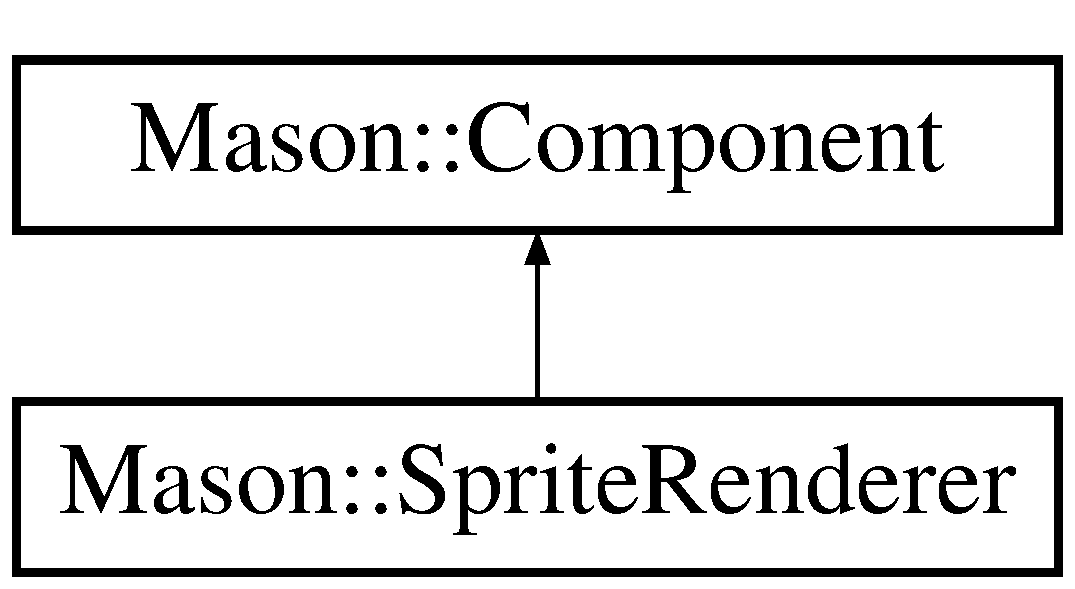
\includegraphics[height=2.000000cm]{class_mason_1_1_sprite_renderer}
\end{center}
\end{figure}
\subsection*{Public Member Functions}
\begin{DoxyCompactItemize}
\item 
void \hyperlink{class_mason_1_1_sprite_renderer_aeeeaa7eb5c340b7c2abad3d4785fd1e1}{draw} ()
\end{DoxyCompactItemize}
\subsection*{Public Attributes}
\begin{DoxyCompactItemize}
\item 
std\+::shared\+\_\+ptr$<$ \hyperlink{class_mason_1_1_sprite}{Sprite} $>$ \hyperlink{class_mason_1_1_sprite_renderer_a17a9d82d45d7ae1058542e5c939122c6}{sprite}
\end{DoxyCompactItemize}
\subsection*{Protected Member Functions}
\begin{DoxyCompactItemize}
\item 
\hyperlink{class_mason_1_1_sprite_renderer_a82f81ad1b56677f6194d91956b213add}{Sprite\+Renderer} (\hyperlink{class_mason_1_1_game_object}{Game\+Object} $\ast$\hyperlink{class_mason_1_1_component_a30030370c35f5562cbbbb0927b0448c8}{game\+Object})
\end{DoxyCompactItemize}
\subsection*{Protected Attributes}
\begin{DoxyCompactItemize}
\item 
std\+::shared\+\_\+ptr$<$ \hyperlink{class_mason_1_1_transform}{Transform} $>$ \hyperlink{class_mason_1_1_sprite_renderer_a6f117cc02c8fc27dac5692a2127bf329}{transform}
\end{DoxyCompactItemize}
\subsection*{Friends}
\begin{DoxyCompactItemize}
\item 
class \hyperlink{class_mason_1_1_sprite_renderer_a00df87c957d8f7ee0fc51f07a0542f4a}{Game\+Object}
\end{DoxyCompactItemize}


\subsection{Constructor \& Destructor Documentation}
\hypertarget{class_mason_1_1_sprite_renderer_a82f81ad1b56677f6194d91956b213add}{}\label{class_mason_1_1_sprite_renderer_a82f81ad1b56677f6194d91956b213add} 
\index{Mason\+::\+Sprite\+Renderer@{Mason\+::\+Sprite\+Renderer}!Sprite\+Renderer@{Sprite\+Renderer}}
\index{Sprite\+Renderer@{Sprite\+Renderer}!Mason\+::\+Sprite\+Renderer@{Mason\+::\+Sprite\+Renderer}}
\subsubsection{\texorpdfstring{Sprite\+Renderer()}{SpriteRenderer()}}
{\footnotesize\ttfamily Sprite\+Renderer\+::\+Sprite\+Renderer (\begin{DoxyParamCaption}\item[{\hyperlink{class_mason_1_1_game_object}{Game\+Object} $\ast$}]{game\+Object }\end{DoxyParamCaption})\hspace{0.3cm}{\ttfamily [protected]}}



\subsection{Member Function Documentation}
\hypertarget{class_mason_1_1_sprite_renderer_aeeeaa7eb5c340b7c2abad3d4785fd1e1}{}\label{class_mason_1_1_sprite_renderer_aeeeaa7eb5c340b7c2abad3d4785fd1e1} 
\index{Mason\+::\+Sprite\+Renderer@{Mason\+::\+Sprite\+Renderer}!draw@{draw}}
\index{draw@{draw}!Mason\+::\+Sprite\+Renderer@{Mason\+::\+Sprite\+Renderer}}
\subsubsection{\texorpdfstring{draw()}{draw()}}
{\footnotesize\ttfamily void Sprite\+Renderer\+::draw (\begin{DoxyParamCaption}{ }\end{DoxyParamCaption})}



\subsection{Friends And Related Function Documentation}
\hypertarget{class_mason_1_1_sprite_renderer_a00df87c957d8f7ee0fc51f07a0542f4a}{}\label{class_mason_1_1_sprite_renderer_a00df87c957d8f7ee0fc51f07a0542f4a} 
\index{Mason\+::\+Sprite\+Renderer@{Mason\+::\+Sprite\+Renderer}!Game\+Object@{Game\+Object}}
\index{Game\+Object@{Game\+Object}!Mason\+::\+Sprite\+Renderer@{Mason\+::\+Sprite\+Renderer}}
\subsubsection{\texorpdfstring{Game\+Object}{GameObject}}
{\footnotesize\ttfamily friend class \hyperlink{class_mason_1_1_game_object}{Game\+Object}\hspace{0.3cm}{\ttfamily [friend]}}



\subsection{Member Data Documentation}
\hypertarget{class_mason_1_1_sprite_renderer_a17a9d82d45d7ae1058542e5c939122c6}{}\label{class_mason_1_1_sprite_renderer_a17a9d82d45d7ae1058542e5c939122c6} 
\index{Mason\+::\+Sprite\+Renderer@{Mason\+::\+Sprite\+Renderer}!sprite@{sprite}}
\index{sprite@{sprite}!Mason\+::\+Sprite\+Renderer@{Mason\+::\+Sprite\+Renderer}}
\subsubsection{\texorpdfstring{sprite}{sprite}}
{\footnotesize\ttfamily std\+::shared\+\_\+ptr$<$\hyperlink{class_mason_1_1_sprite}{Sprite}$>$ Mason\+::\+Sprite\+Renderer\+::sprite}

\hypertarget{class_mason_1_1_sprite_renderer_a6f117cc02c8fc27dac5692a2127bf329}{}\label{class_mason_1_1_sprite_renderer_a6f117cc02c8fc27dac5692a2127bf329} 
\index{Mason\+::\+Sprite\+Renderer@{Mason\+::\+Sprite\+Renderer}!transform@{transform}}
\index{transform@{transform}!Mason\+::\+Sprite\+Renderer@{Mason\+::\+Sprite\+Renderer}}
\subsubsection{\texorpdfstring{transform}{transform}}
{\footnotesize\ttfamily std\+::shared\+\_\+ptr$<$\hyperlink{class_mason_1_1_transform}{Transform}$>$ Mason\+::\+Sprite\+Renderer\+::transform\hspace{0.3cm}{\ttfamily [protected]}}



The documentation for this class was generated from the following files\+:\begin{DoxyCompactItemize}
\item 
C\+:/\+Users/\+Carol/\+Documents/\+Git\+Hub/\+Team\+Does\+Not\+Matter/\+Engine/include/\+Mason/\hyperlink{_sprite_renderer_8h}{Sprite\+Renderer.\+h}\item 
C\+:/\+Users/\+Carol/\+Documents/\+Git\+Hub/\+Team\+Does\+Not\+Matter/\+Engine/src/\hyperlink{_sprite_renderer_8cpp}{Sprite\+Renderer.\+cpp}\end{DoxyCompactItemize}

\hypertarget{class_s_r_e_debug_draw}{}\section{S\+R\+E\+Debug\+Draw Class Reference}
\label{class_s_r_e_debug_draw}\index{S\+R\+E\+Debug\+Draw@{S\+R\+E\+Debug\+Draw}}


{\ttfamily \#include $<$S\+R\+E\+Debug\+Draw.\+h$>$}

Inheritance diagram for S\+R\+E\+Debug\+Draw\+:\begin{figure}[H]
\begin{center}
\leavevmode
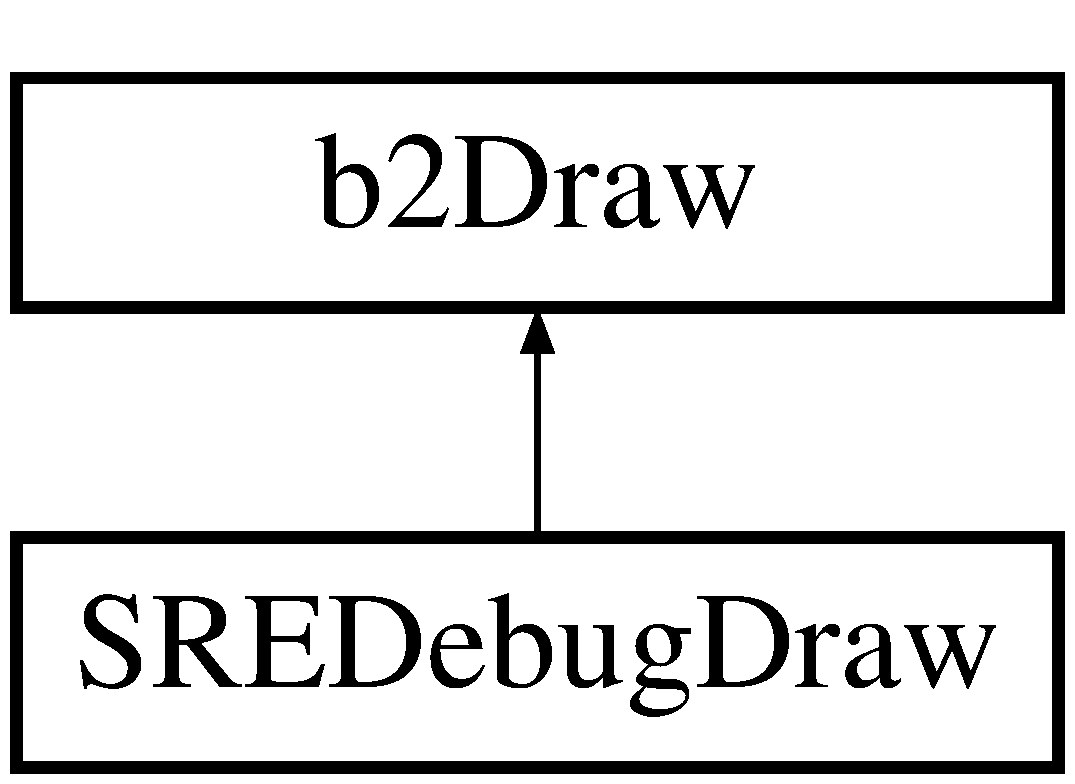
\includegraphics[height=2.000000cm]{class_s_r_e_debug_draw}
\end{center}
\end{figure}
\subsection*{Public Member Functions}
\begin{DoxyCompactItemize}
\item 
\hyperlink{class_s_r_e_debug_draw_a6b4f4f7d72bb85ea3bfecd282786693a}{S\+R\+E\+Debug\+Draw} ()
\item 
void \hyperlink{class_s_r_e_debug_draw_a3aeb14dc08bb5c4d490e30cc62ad1787}{Draw\+Polygon} (const b2\+Vec2 $\ast$vertices, int32 vertex\+Count, const b2\+Color \&color)
\item 
void \hyperlink{class_s_r_e_debug_draw_af8308d695e1c6b61a2ba4226921c6b70}{Draw\+Solid\+Polygon} (const b2\+Vec2 $\ast$vertices, int32 vertex\+Count, const b2\+Color \&color)
\item 
void \hyperlink{class_s_r_e_debug_draw_a6cb71e10d252900e6f469389146b9f48}{Draw\+Circle} (const b2\+Vec2 \&center, float32 radius, const b2\+Color \&color)
\item 
void \hyperlink{class_s_r_e_debug_draw_a9392357bb882d28ca0a86f179901488b}{Draw\+Solid\+Circle} (const b2\+Vec2 \&center, float32 radius, const b2\+Vec2 \&axis, const b2\+Color \&color)
\item 
void \hyperlink{class_s_r_e_debug_draw_ae52016e6134930d09f6f8a07308cc9e7}{Draw\+Segment} (const b2\+Vec2 \&p1, const b2\+Vec2 \&p2, const b2\+Color \&color)
\item 
void \hyperlink{class_s_r_e_debug_draw_aaa826d0f196accca390c47023d28e2ce}{Draw\+Point} (const b2\+Vec2 \&p, float32 size, const b2\+Color \&color)
\item 
void \hyperlink{class_s_r_e_debug_draw_a5255695e40bf3418a9f68e1405822aeb}{Draw\+Transform} (const b2\+Transform \&xf)
\end{DoxyCompactItemize}


\subsection{Constructor \& Destructor Documentation}
\hypertarget{class_s_r_e_debug_draw_a6b4f4f7d72bb85ea3bfecd282786693a}{}\label{class_s_r_e_debug_draw_a6b4f4f7d72bb85ea3bfecd282786693a} 
\index{S\+R\+E\+Debug\+Draw@{S\+R\+E\+Debug\+Draw}!S\+R\+E\+Debug\+Draw@{S\+R\+E\+Debug\+Draw}}
\index{S\+R\+E\+Debug\+Draw@{S\+R\+E\+Debug\+Draw}!S\+R\+E\+Debug\+Draw@{S\+R\+E\+Debug\+Draw}}
\subsubsection{\texorpdfstring{S\+R\+E\+Debug\+Draw()}{SREDebugDraw()}}
{\footnotesize\ttfamily S\+R\+E\+Debug\+Draw\+::\+S\+R\+E\+Debug\+Draw (\begin{DoxyParamCaption}{ }\end{DoxyParamCaption})}



\subsection{Member Function Documentation}
\hypertarget{class_s_r_e_debug_draw_a6cb71e10d252900e6f469389146b9f48}{}\label{class_s_r_e_debug_draw_a6cb71e10d252900e6f469389146b9f48} 
\index{S\+R\+E\+Debug\+Draw@{S\+R\+E\+Debug\+Draw}!Draw\+Circle@{Draw\+Circle}}
\index{Draw\+Circle@{Draw\+Circle}!S\+R\+E\+Debug\+Draw@{S\+R\+E\+Debug\+Draw}}
\subsubsection{\texorpdfstring{Draw\+Circle()}{DrawCircle()}}
{\footnotesize\ttfamily void S\+R\+E\+Debug\+Draw\+::\+Draw\+Circle (\begin{DoxyParamCaption}\item[{const b2\+Vec2 \&}]{center,  }\item[{float32}]{radius,  }\item[{const b2\+Color \&}]{color }\end{DoxyParamCaption})}

\hypertarget{class_s_r_e_debug_draw_aaa826d0f196accca390c47023d28e2ce}{}\label{class_s_r_e_debug_draw_aaa826d0f196accca390c47023d28e2ce} 
\index{S\+R\+E\+Debug\+Draw@{S\+R\+E\+Debug\+Draw}!Draw\+Point@{Draw\+Point}}
\index{Draw\+Point@{Draw\+Point}!S\+R\+E\+Debug\+Draw@{S\+R\+E\+Debug\+Draw}}
\subsubsection{\texorpdfstring{Draw\+Point()}{DrawPoint()}}
{\footnotesize\ttfamily void S\+R\+E\+Debug\+Draw\+::\+Draw\+Point (\begin{DoxyParamCaption}\item[{const b2\+Vec2 \&}]{p,  }\item[{float32}]{size,  }\item[{const b2\+Color \&}]{color }\end{DoxyParamCaption})}

\hypertarget{class_s_r_e_debug_draw_a3aeb14dc08bb5c4d490e30cc62ad1787}{}\label{class_s_r_e_debug_draw_a3aeb14dc08bb5c4d490e30cc62ad1787} 
\index{S\+R\+E\+Debug\+Draw@{S\+R\+E\+Debug\+Draw}!Draw\+Polygon@{Draw\+Polygon}}
\index{Draw\+Polygon@{Draw\+Polygon}!S\+R\+E\+Debug\+Draw@{S\+R\+E\+Debug\+Draw}}
\subsubsection{\texorpdfstring{Draw\+Polygon()}{DrawPolygon()}}
{\footnotesize\ttfamily void S\+R\+E\+Debug\+Draw\+::\+Draw\+Polygon (\begin{DoxyParamCaption}\item[{const b2\+Vec2 $\ast$}]{vertices,  }\item[{int32}]{vertex\+Count,  }\item[{const b2\+Color \&}]{color }\end{DoxyParamCaption})}

\hypertarget{class_s_r_e_debug_draw_ae52016e6134930d09f6f8a07308cc9e7}{}\label{class_s_r_e_debug_draw_ae52016e6134930d09f6f8a07308cc9e7} 
\index{S\+R\+E\+Debug\+Draw@{S\+R\+E\+Debug\+Draw}!Draw\+Segment@{Draw\+Segment}}
\index{Draw\+Segment@{Draw\+Segment}!S\+R\+E\+Debug\+Draw@{S\+R\+E\+Debug\+Draw}}
\subsubsection{\texorpdfstring{Draw\+Segment()}{DrawSegment()}}
{\footnotesize\ttfamily void S\+R\+E\+Debug\+Draw\+::\+Draw\+Segment (\begin{DoxyParamCaption}\item[{const b2\+Vec2 \&}]{p1,  }\item[{const b2\+Vec2 \&}]{p2,  }\item[{const b2\+Color \&}]{color }\end{DoxyParamCaption})}

\hypertarget{class_s_r_e_debug_draw_a9392357bb882d28ca0a86f179901488b}{}\label{class_s_r_e_debug_draw_a9392357bb882d28ca0a86f179901488b} 
\index{S\+R\+E\+Debug\+Draw@{S\+R\+E\+Debug\+Draw}!Draw\+Solid\+Circle@{Draw\+Solid\+Circle}}
\index{Draw\+Solid\+Circle@{Draw\+Solid\+Circle}!S\+R\+E\+Debug\+Draw@{S\+R\+E\+Debug\+Draw}}
\subsubsection{\texorpdfstring{Draw\+Solid\+Circle()}{DrawSolidCircle()}}
{\footnotesize\ttfamily void S\+R\+E\+Debug\+Draw\+::\+Draw\+Solid\+Circle (\begin{DoxyParamCaption}\item[{const b2\+Vec2 \&}]{center,  }\item[{float32}]{radius,  }\item[{const b2\+Vec2 \&}]{axis,  }\item[{const b2\+Color \&}]{color }\end{DoxyParamCaption})}

\hypertarget{class_s_r_e_debug_draw_af8308d695e1c6b61a2ba4226921c6b70}{}\label{class_s_r_e_debug_draw_af8308d695e1c6b61a2ba4226921c6b70} 
\index{S\+R\+E\+Debug\+Draw@{S\+R\+E\+Debug\+Draw}!Draw\+Solid\+Polygon@{Draw\+Solid\+Polygon}}
\index{Draw\+Solid\+Polygon@{Draw\+Solid\+Polygon}!S\+R\+E\+Debug\+Draw@{S\+R\+E\+Debug\+Draw}}
\subsubsection{\texorpdfstring{Draw\+Solid\+Polygon()}{DrawSolidPolygon()}}
{\footnotesize\ttfamily void S\+R\+E\+Debug\+Draw\+::\+Draw\+Solid\+Polygon (\begin{DoxyParamCaption}\item[{const b2\+Vec2 $\ast$}]{vertices,  }\item[{int32}]{vertex\+Count,  }\item[{const b2\+Color \&}]{color }\end{DoxyParamCaption})}

\hypertarget{class_s_r_e_debug_draw_a5255695e40bf3418a9f68e1405822aeb}{}\label{class_s_r_e_debug_draw_a5255695e40bf3418a9f68e1405822aeb} 
\index{S\+R\+E\+Debug\+Draw@{S\+R\+E\+Debug\+Draw}!Draw\+Transform@{Draw\+Transform}}
\index{Draw\+Transform@{Draw\+Transform}!S\+R\+E\+Debug\+Draw@{S\+R\+E\+Debug\+Draw}}
\subsubsection{\texorpdfstring{Draw\+Transform()}{DrawTransform()}}
{\footnotesize\ttfamily void S\+R\+E\+Debug\+Draw\+::\+Draw\+Transform (\begin{DoxyParamCaption}\item[{const b2\+Transform \&}]{xf }\end{DoxyParamCaption})}



The documentation for this class was generated from the following files\+:\begin{DoxyCompactItemize}
\item 
C\+:/\+Users/\+Carol/\+Documents/\+Git\+Hub/\+Team\+Does\+Not\+Matter/\+Engine/include/\+Mason/\hyperlink{_s_r_e_debug_draw_8h}{S\+R\+E\+Debug\+Draw.\+h}\item 
C\+:/\+Users/\+Carol/\+Documents/\+Git\+Hub/\+Team\+Does\+Not\+Matter/\+Engine/src/\hyperlink{_s_r_e_debug_draw_8cpp}{S\+R\+E\+Debug\+Draw.\+cpp}\end{DoxyCompactItemize}

\hypertarget{class_mason_1_1_time}{}\section{Mason\+:\+:Time Class Reference}
\label{class_mason_1_1_time}\index{Mason\+::\+Time@{Mason\+::\+Time}}


{\ttfamily \#include $<$Time.\+hpp$>$}

\subsection*{Static Public Member Functions}
\begin{DoxyCompactItemize}
\item 
static float \hyperlink{class_mason_1_1_time_ad6773c7a2339b463fc7ea14e31315c89}{get\+Time} ()
\item 
static float \hyperlink{class_mason_1_1_time_a405c7642c4ba0ee719a8d0491099102a}{get\+Delta\+Time} ()
\end{DoxyCompactItemize}


\subsection{Member Function Documentation}
\hypertarget{class_mason_1_1_time_a405c7642c4ba0ee719a8d0491099102a}{}\label{class_mason_1_1_time_a405c7642c4ba0ee719a8d0491099102a} 
\index{Mason\+::\+Time@{Mason\+::\+Time}!get\+Delta\+Time@{get\+Delta\+Time}}
\index{get\+Delta\+Time@{get\+Delta\+Time}!Mason\+::\+Time@{Mason\+::\+Time}}
\subsubsection{\texorpdfstring{get\+Delta\+Time()}{getDeltaTime()}}
{\footnotesize\ttfamily float Time\+::get\+Delta\+Time (\begin{DoxyParamCaption}{ }\end{DoxyParamCaption})\hspace{0.3cm}{\ttfamily [static]}}

\hypertarget{class_mason_1_1_time_ad6773c7a2339b463fc7ea14e31315c89}{}\label{class_mason_1_1_time_ad6773c7a2339b463fc7ea14e31315c89} 
\index{Mason\+::\+Time@{Mason\+::\+Time}!get\+Time@{get\+Time}}
\index{get\+Time@{get\+Time}!Mason\+::\+Time@{Mason\+::\+Time}}
\subsubsection{\texorpdfstring{get\+Time()}{getTime()}}
{\footnotesize\ttfamily float Time\+::get\+Time (\begin{DoxyParamCaption}{ }\end{DoxyParamCaption})\hspace{0.3cm}{\ttfamily [static]}}



The documentation for this class was generated from the following files\+:\begin{DoxyCompactItemize}
\item 
include/\+Mason/\hyperlink{_time_8hpp}{Time.\+hpp}\item 
src/\hyperlink{_time_8cpp}{Time.\+cpp}\end{DoxyCompactItemize}

\hypertarget{class_mason_1_1_transform}{}\section{Mason\+:\+:Transform Class Reference}
\label{class_mason_1_1_transform}\index{Mason\+::\+Transform@{Mason\+::\+Transform}}


{\ttfamily \#include $<$Transform.\+h$>$}



Inheritance diagram for Mason\+:\+:Transform\+:
% FIG 0


Collaboration diagram for Mason\+:\+:Transform\+:
% FIG 1
\subsection*{Public Member Functions}
\begin{DoxyCompactItemize}
\item 
virtual void \hyperlink{class_mason_1_1_transform_a740f389e20c0190c52bcb893aeaa0490}{set\+Position} (glm\+::vec3 \hyperlink{class_mason_1_1_transform_ac9e11b4ec4433a38ac1100f12c955dcb}{position})
\item 
virtual void \hyperlink{class_mason_1_1_transform_aacc2b668bdd1d9b978aa0edccf75144a}{set\+Rotation} (glm\+::vec3 \hyperlink{class_mason_1_1_transform_ae2f541ade79d561584619e93edb034ae}{rotation})
\item 
virtual void \hyperlink{class_mason_1_1_transform_a4a273ac58f45b6ee9cf2b37cf661daac}{set\+Scale} (glm\+::vec3 \hyperlink{class_mason_1_1_transform_a4618b31e34a6ec8a0ee638401fc56367}{scale})
\item 
virtual void \hyperlink{class_mason_1_1_transform_a6e1a6b57214a7de21595e6af8b05138b}{set\+Parent} (\hyperlink{class_mason_1_1_transform}{Transform} $\ast$\hyperlink{class_mason_1_1_component_a30030370c35f5562cbbbb0927b0448c8}{game\+Object})
\item 
virtual glm\+::vec3 \hyperlink{class_mason_1_1_transform_a0b21f641e72d7b55f3a630b986d0b106}{get\+Position} ()
\item 
virtual glm\+::vec3 \hyperlink{class_mason_1_1_transform_a7367502d4344eff2d88a250084ae19dc}{get\+Rotation} ()
\item 
virtual glm\+::vec3 \hyperlink{class_mason_1_1_transform_a24107560725b250c4c2e10ab98a6ac04}{get\+Scale} ()
\item 
virtual \hyperlink{class_mason_1_1_transform}{Transform} $\ast$ \hyperlink{class_mason_1_1_transform_ae3e8acbd25d7d171aff00da038f79a9a}{get\+Parent} ()
\item 
glm\+::mat4 \hyperlink{class_mason_1_1_transform_a8b85abc03488f58bef8bb78df77c1689}{local\+Transform} ()
\item 
glm\+::mat4 \hyperlink{class_mason_1_1_transform_a35e627aa09604bf3a81f4c07d28205f3}{global\+Transform} ()
\end{DoxyCompactItemize}
\subsection*{Protected Member Functions}
\begin{DoxyCompactItemize}
\item 
\hyperlink{class_mason_1_1_transform_a00209266b27fa0c297551a0ce4a07017}{Transform} (\hyperlink{class_mason_1_1_game_object}{Game\+Object} $\ast$\hyperlink{class_mason_1_1_component_a30030370c35f5562cbbbb0927b0448c8}{game\+Object})
\item 
virtual void \hyperlink{class_mason_1_1_transform_a4dd61568d49044377f3312397ffdafd1}{transformize} ()
\end{DoxyCompactItemize}
\subsection*{Protected Attributes}
\begin{DoxyCompactItemize}
\item 
glm\+::mat4 \hyperlink{class_mason_1_1_transform_aeb64a62787375e23645da6f490763c25}{matrix}
\item 
glm\+::vec3 \hyperlink{class_mason_1_1_transform_ac9e11b4ec4433a38ac1100f12c955dcb}{position}
\item 
glm\+::vec3 \hyperlink{class_mason_1_1_transform_ae2f541ade79d561584619e93edb034ae}{rotation}
\item 
glm\+::vec3 \hyperlink{class_mason_1_1_transform_a4618b31e34a6ec8a0ee638401fc56367}{scale}
\item 
\hyperlink{class_mason_1_1_transform}{Transform} $\ast$ \hyperlink{class_mason_1_1_transform_a1e2c91adcef43bcc170803656260f9db}{parent}
\end{DoxyCompactItemize}
\subsection*{Friends}
\begin{DoxyCompactItemize}
\item 
class \hyperlink{class_mason_1_1_transform_a00df87c957d8f7ee0fc51f07a0542f4a}{Game\+Object}
\item 
class \hyperlink{class_mason_1_1_transform_a33061a25b8332281d02c83e2bf1d4959}{Rendering}
\item 
class \hyperlink{class_mason_1_1_transform_a82b374d797a09668286ac5cf26f539f3}{Particle\+Emitter}
\end{DoxyCompactItemize}


\subsection{Constructor \& Destructor Documentation}
\hypertarget{class_mason_1_1_transform_a00209266b27fa0c297551a0ce4a07017}{}\label{class_mason_1_1_transform_a00209266b27fa0c297551a0ce4a07017} 
\index{Mason\+::\+Transform@{Mason\+::\+Transform}!Transform@{Transform}}
\index{Transform@{Transform}!Mason\+::\+Transform@{Mason\+::\+Transform}}
\subsubsection{\texorpdfstring{Transform()}{Transform()}}
{\footnotesize\ttfamily Transform\+::\+Transform (\begin{DoxyParamCaption}\item[{\hyperlink{class_mason_1_1_game_object}{Game\+Object} $\ast$}]{game\+Object }\end{DoxyParamCaption})\hspace{0.3cm}{\ttfamily [protected]}}



\subsection{Member Function Documentation}
\hypertarget{class_mason_1_1_transform_ae3e8acbd25d7d171aff00da038f79a9a}{}\label{class_mason_1_1_transform_ae3e8acbd25d7d171aff00da038f79a9a} 
\index{Mason\+::\+Transform@{Mason\+::\+Transform}!get\+Parent@{get\+Parent}}
\index{get\+Parent@{get\+Parent}!Mason\+::\+Transform@{Mason\+::\+Transform}}
\subsubsection{\texorpdfstring{get\+Parent()}{getParent()}}
{\footnotesize\ttfamily \hyperlink{class_mason_1_1_transform}{Transform} $\ast$ Transform\+::get\+Parent (\begin{DoxyParamCaption}{ }\end{DoxyParamCaption})\hspace{0.3cm}{\ttfamily [virtual]}}

\hypertarget{class_mason_1_1_transform_a0b21f641e72d7b55f3a630b986d0b106}{}\label{class_mason_1_1_transform_a0b21f641e72d7b55f3a630b986d0b106} 
\index{Mason\+::\+Transform@{Mason\+::\+Transform}!get\+Position@{get\+Position}}
\index{get\+Position@{get\+Position}!Mason\+::\+Transform@{Mason\+::\+Transform}}
\subsubsection{\texorpdfstring{get\+Position()}{getPosition()}}
{\footnotesize\ttfamily glm\+::vec3 Transform\+::get\+Position (\begin{DoxyParamCaption}{ }\end{DoxyParamCaption})\hspace{0.3cm}{\ttfamily [virtual]}}



Reimplemented in \hyperlink{class_mason_1_1_camera_a71560b8b6216a542ae1958bd91a4361d}{Mason\+::\+Camera}.

\hypertarget{class_mason_1_1_transform_a7367502d4344eff2d88a250084ae19dc}{}\label{class_mason_1_1_transform_a7367502d4344eff2d88a250084ae19dc} 
\index{Mason\+::\+Transform@{Mason\+::\+Transform}!get\+Rotation@{get\+Rotation}}
\index{get\+Rotation@{get\+Rotation}!Mason\+::\+Transform@{Mason\+::\+Transform}}
\subsubsection{\texorpdfstring{get\+Rotation()}{getRotation()}}
{\footnotesize\ttfamily glm\+::vec3 Transform\+::get\+Rotation (\begin{DoxyParamCaption}{ }\end{DoxyParamCaption})\hspace{0.3cm}{\ttfamily [virtual]}}

\hypertarget{class_mason_1_1_transform_a24107560725b250c4c2e10ab98a6ac04}{}\label{class_mason_1_1_transform_a24107560725b250c4c2e10ab98a6ac04} 
\index{Mason\+::\+Transform@{Mason\+::\+Transform}!get\+Scale@{get\+Scale}}
\index{get\+Scale@{get\+Scale}!Mason\+::\+Transform@{Mason\+::\+Transform}}
\subsubsection{\texorpdfstring{get\+Scale()}{getScale()}}
{\footnotesize\ttfamily glm\+::vec3 Transform\+::get\+Scale (\begin{DoxyParamCaption}{ }\end{DoxyParamCaption})\hspace{0.3cm}{\ttfamily [virtual]}}



Reimplemented in \hyperlink{class_mason_1_1_camera_a405b26eaaae2ab7a460dfc319a9d16ea}{Mason\+::\+Camera}.

\hypertarget{class_mason_1_1_transform_a35e627aa09604bf3a81f4c07d28205f3}{}\label{class_mason_1_1_transform_a35e627aa09604bf3a81f4c07d28205f3} 
\index{Mason\+::\+Transform@{Mason\+::\+Transform}!global\+Transform@{global\+Transform}}
\index{global\+Transform@{global\+Transform}!Mason\+::\+Transform@{Mason\+::\+Transform}}
\subsubsection{\texorpdfstring{global\+Transform()}{globalTransform()}}
{\footnotesize\ttfamily glm\+::mat4 Transform\+::global\+Transform (\begin{DoxyParamCaption}{ }\end{DoxyParamCaption})}

Here is the call graph for this function\+:
% FIG 2
\hypertarget{class_mason_1_1_transform_a8b85abc03488f58bef8bb78df77c1689}{}\label{class_mason_1_1_transform_a8b85abc03488f58bef8bb78df77c1689} 
\index{Mason\+::\+Transform@{Mason\+::\+Transform}!local\+Transform@{local\+Transform}}
\index{local\+Transform@{local\+Transform}!Mason\+::\+Transform@{Mason\+::\+Transform}}
\subsubsection{\texorpdfstring{local\+Transform()}{localTransform()}}
{\footnotesize\ttfamily glm\+::mat4 Transform\+::local\+Transform (\begin{DoxyParamCaption}{ }\end{DoxyParamCaption})}

\hypertarget{class_mason_1_1_transform_a6e1a6b57214a7de21595e6af8b05138b}{}\label{class_mason_1_1_transform_a6e1a6b57214a7de21595e6af8b05138b} 
\index{Mason\+::\+Transform@{Mason\+::\+Transform}!set\+Parent@{set\+Parent}}
\index{set\+Parent@{set\+Parent}!Mason\+::\+Transform@{Mason\+::\+Transform}}
\subsubsection{\texorpdfstring{set\+Parent()}{setParent()}}
{\footnotesize\ttfamily void Transform\+::set\+Parent (\begin{DoxyParamCaption}\item[{\hyperlink{class_mason_1_1_transform}{Transform} $\ast$}]{game\+Object }\end{DoxyParamCaption})\hspace{0.3cm}{\ttfamily [virtual]}}

\hypertarget{class_mason_1_1_transform_a740f389e20c0190c52bcb893aeaa0490}{}\label{class_mason_1_1_transform_a740f389e20c0190c52bcb893aeaa0490} 
\index{Mason\+::\+Transform@{Mason\+::\+Transform}!set\+Position@{set\+Position}}
\index{set\+Position@{set\+Position}!Mason\+::\+Transform@{Mason\+::\+Transform}}
\subsubsection{\texorpdfstring{set\+Position()}{setPosition()}}
{\footnotesize\ttfamily void Transform\+::set\+Position (\begin{DoxyParamCaption}\item[{glm\+::vec3}]{position }\end{DoxyParamCaption})\hspace{0.3cm}{\ttfamily [virtual]}}



Reimplemented in \hyperlink{class_mason_1_1_camera_a69f184af46d081b85209040bbe814cbb}{Mason\+::\+Camera}.

Here is the call graph for this function\+:
% FIG 3
\hypertarget{class_mason_1_1_transform_aacc2b668bdd1d9b978aa0edccf75144a}{}\label{class_mason_1_1_transform_aacc2b668bdd1d9b978aa0edccf75144a} 
\index{Mason\+::\+Transform@{Mason\+::\+Transform}!set\+Rotation@{set\+Rotation}}
\index{set\+Rotation@{set\+Rotation}!Mason\+::\+Transform@{Mason\+::\+Transform}}
\subsubsection{\texorpdfstring{set\+Rotation()}{setRotation()}}
{\footnotesize\ttfamily void Transform\+::set\+Rotation (\begin{DoxyParamCaption}\item[{glm\+::vec3}]{rotation }\end{DoxyParamCaption})\hspace{0.3cm}{\ttfamily [virtual]}}

Here is the call graph for this function\+:
% FIG 4
\hypertarget{class_mason_1_1_transform_a4a273ac58f45b6ee9cf2b37cf661daac}{}\label{class_mason_1_1_transform_a4a273ac58f45b6ee9cf2b37cf661daac} 
\index{Mason\+::\+Transform@{Mason\+::\+Transform}!set\+Scale@{set\+Scale}}
\index{set\+Scale@{set\+Scale}!Mason\+::\+Transform@{Mason\+::\+Transform}}
\subsubsection{\texorpdfstring{set\+Scale()}{setScale()}}
{\footnotesize\ttfamily void Transform\+::set\+Scale (\begin{DoxyParamCaption}\item[{glm\+::vec3}]{scale }\end{DoxyParamCaption})\hspace{0.3cm}{\ttfamily [virtual]}}



Reimplemented in \hyperlink{class_mason_1_1_camera_a732501ee31e862f557bbbc8ff58631a4}{Mason\+::\+Camera}.

Here is the call graph for this function\+:
% FIG 5
\hypertarget{class_mason_1_1_transform_a4dd61568d49044377f3312397ffdafd1}{}\label{class_mason_1_1_transform_a4dd61568d49044377f3312397ffdafd1} 
\index{Mason\+::\+Transform@{Mason\+::\+Transform}!transformize@{transformize}}
\index{transformize@{transformize}!Mason\+::\+Transform@{Mason\+::\+Transform}}
\subsubsection{\texorpdfstring{transformize()}{transformize()}}
{\footnotesize\ttfamily void Transform\+::transformize (\begin{DoxyParamCaption}{ }\end{DoxyParamCaption})\hspace{0.3cm}{\ttfamily [protected]}, {\ttfamily [virtual]}}



Reimplemented in \hyperlink{class_mason_1_1_camera_a27ff2d3ad004a49db2ae508ac6e9d3c2}{Mason\+::\+Camera}.



\subsection{Friends And Related Function Documentation}
\hypertarget{class_mason_1_1_transform_a00df87c957d8f7ee0fc51f07a0542f4a}{}\label{class_mason_1_1_transform_a00df87c957d8f7ee0fc51f07a0542f4a} 
\index{Mason\+::\+Transform@{Mason\+::\+Transform}!Game\+Object@{Game\+Object}}
\index{Game\+Object@{Game\+Object}!Mason\+::\+Transform@{Mason\+::\+Transform}}
\subsubsection{\texorpdfstring{Game\+Object}{GameObject}}
{\footnotesize\ttfamily friend class \hyperlink{class_mason_1_1_game_object}{Game\+Object}\hspace{0.3cm}{\ttfamily [friend]}}

\hypertarget{class_mason_1_1_transform_a82b374d797a09668286ac5cf26f539f3}{}\label{class_mason_1_1_transform_a82b374d797a09668286ac5cf26f539f3} 
\index{Mason\+::\+Transform@{Mason\+::\+Transform}!Particle\+Emitter@{Particle\+Emitter}}
\index{Particle\+Emitter@{Particle\+Emitter}!Mason\+::\+Transform@{Mason\+::\+Transform}}
\subsubsection{\texorpdfstring{Particle\+Emitter}{ParticleEmitter}}
{\footnotesize\ttfamily friend class \hyperlink{class_mason_1_1_particle_emitter}{Particle\+Emitter}\hspace{0.3cm}{\ttfamily [friend]}}

\hypertarget{class_mason_1_1_transform_a33061a25b8332281d02c83e2bf1d4959}{}\label{class_mason_1_1_transform_a33061a25b8332281d02c83e2bf1d4959} 
\index{Mason\+::\+Transform@{Mason\+::\+Transform}!Rendering@{Rendering}}
\index{Rendering@{Rendering}!Mason\+::\+Transform@{Mason\+::\+Transform}}
\subsubsection{\texorpdfstring{Rendering}{Rendering}}
{\footnotesize\ttfamily friend class Rendering\hspace{0.3cm}{\ttfamily [friend]}}



\subsection{Member Data Documentation}
\hypertarget{class_mason_1_1_transform_aeb64a62787375e23645da6f490763c25}{}\label{class_mason_1_1_transform_aeb64a62787375e23645da6f490763c25} 
\index{Mason\+::\+Transform@{Mason\+::\+Transform}!matrix@{matrix}}
\index{matrix@{matrix}!Mason\+::\+Transform@{Mason\+::\+Transform}}
\subsubsection{\texorpdfstring{matrix}{matrix}}
{\footnotesize\ttfamily glm\+::mat4 Mason\+::\+Transform\+::matrix\hspace{0.3cm}{\ttfamily [protected]}}

\hypertarget{class_mason_1_1_transform_a1e2c91adcef43bcc170803656260f9db}{}\label{class_mason_1_1_transform_a1e2c91adcef43bcc170803656260f9db} 
\index{Mason\+::\+Transform@{Mason\+::\+Transform}!parent@{parent}}
\index{parent@{parent}!Mason\+::\+Transform@{Mason\+::\+Transform}}
\subsubsection{\texorpdfstring{parent}{parent}}
{\footnotesize\ttfamily \hyperlink{class_mason_1_1_transform}{Transform}$\ast$ Mason\+::\+Transform\+::parent\hspace{0.3cm}{\ttfamily [protected]}}

\hypertarget{class_mason_1_1_transform_ac9e11b4ec4433a38ac1100f12c955dcb}{}\label{class_mason_1_1_transform_ac9e11b4ec4433a38ac1100f12c955dcb} 
\index{Mason\+::\+Transform@{Mason\+::\+Transform}!position@{position}}
\index{position@{position}!Mason\+::\+Transform@{Mason\+::\+Transform}}
\subsubsection{\texorpdfstring{position}{position}}
{\footnotesize\ttfamily glm\+::vec3 Mason\+::\+Transform\+::position\hspace{0.3cm}{\ttfamily [protected]}}

\hypertarget{class_mason_1_1_transform_ae2f541ade79d561584619e93edb034ae}{}\label{class_mason_1_1_transform_ae2f541ade79d561584619e93edb034ae} 
\index{Mason\+::\+Transform@{Mason\+::\+Transform}!rotation@{rotation}}
\index{rotation@{rotation}!Mason\+::\+Transform@{Mason\+::\+Transform}}
\subsubsection{\texorpdfstring{rotation}{rotation}}
{\footnotesize\ttfamily glm\+::vec3 Mason\+::\+Transform\+::rotation\hspace{0.3cm}{\ttfamily [protected]}}

\hypertarget{class_mason_1_1_transform_a4618b31e34a6ec8a0ee638401fc56367}{}\label{class_mason_1_1_transform_a4618b31e34a6ec8a0ee638401fc56367} 
\index{Mason\+::\+Transform@{Mason\+::\+Transform}!scale@{scale}}
\index{scale@{scale}!Mason\+::\+Transform@{Mason\+::\+Transform}}
\subsubsection{\texorpdfstring{scale}{scale}}
{\footnotesize\ttfamily glm\+::vec3 Mason\+::\+Transform\+::scale\hspace{0.3cm}{\ttfamily [protected]}}



The documentation for this class was generated from the following files\+:\begin{DoxyCompactItemize}
\item 
include/\+Mason/\hyperlink{_transform_8h}{Transform.\+h}\item 
src/\hyperlink{_transform_8cpp}{Transform.\+cpp}\end{DoxyCompactItemize}

\hypertarget{class_mason_1_1_transform_descriptor}{}\section{Mason\+:\+:Transform\+Descriptor Class Reference}
\label{class_mason_1_1_transform_descriptor}\index{Mason\+::\+Transform\+Descriptor@{Mason\+::\+Transform\+Descriptor}}


{\ttfamily \#include $<$Scene\+Parser.\+hpp$>$}

\subsection*{Public Attributes}
\begin{DoxyCompactItemize}
\item 
glm\+::vec3 \hyperlink{class_mason_1_1_transform_descriptor_acce622c3f89ae5b081c61feabc1319bf}{position} = glm\+::vec3(0, 0, 0)
\item 
glm\+::vec3 \hyperlink{class_mason_1_1_transform_descriptor_aa66cc703fd520b19b4347b390eabfc41}{rotation\+Euler} = glm\+::vec3(0, 0, 0)
\item 
glm\+::vec3 \hyperlink{class_mason_1_1_transform_descriptor_a5d264880a0c22c624c996057bf59b752}{scale} = glm\+::vec3(1, 1, 1)
\item 
int \hyperlink{class_mason_1_1_transform_descriptor_ae83bf1f16969979cb24e2ae9d1eb3134}{parent\+Id} = -\/1
\end{DoxyCompactItemize}


\subsection{Member Data Documentation}
\hypertarget{class_mason_1_1_transform_descriptor_ae83bf1f16969979cb24e2ae9d1eb3134}{}\label{class_mason_1_1_transform_descriptor_ae83bf1f16969979cb24e2ae9d1eb3134} 
\index{Mason\+::\+Transform\+Descriptor@{Mason\+::\+Transform\+Descriptor}!parent\+Id@{parent\+Id}}
\index{parent\+Id@{parent\+Id}!Mason\+::\+Transform\+Descriptor@{Mason\+::\+Transform\+Descriptor}}
\subsubsection{\texorpdfstring{parent\+Id}{parentId}}
{\footnotesize\ttfamily int Mason\+::\+Transform\+Descriptor\+::parent\+Id = -\/1}

\hypertarget{class_mason_1_1_transform_descriptor_acce622c3f89ae5b081c61feabc1319bf}{}\label{class_mason_1_1_transform_descriptor_acce622c3f89ae5b081c61feabc1319bf} 
\index{Mason\+::\+Transform\+Descriptor@{Mason\+::\+Transform\+Descriptor}!position@{position}}
\index{position@{position}!Mason\+::\+Transform\+Descriptor@{Mason\+::\+Transform\+Descriptor}}
\subsubsection{\texorpdfstring{position}{position}}
{\footnotesize\ttfamily glm\+::vec3 Mason\+::\+Transform\+Descriptor\+::position = glm\+::vec3(0, 0, 0)}

\hypertarget{class_mason_1_1_transform_descriptor_aa66cc703fd520b19b4347b390eabfc41}{}\label{class_mason_1_1_transform_descriptor_aa66cc703fd520b19b4347b390eabfc41} 
\index{Mason\+::\+Transform\+Descriptor@{Mason\+::\+Transform\+Descriptor}!rotation\+Euler@{rotation\+Euler}}
\index{rotation\+Euler@{rotation\+Euler}!Mason\+::\+Transform\+Descriptor@{Mason\+::\+Transform\+Descriptor}}
\subsubsection{\texorpdfstring{rotation\+Euler}{rotationEuler}}
{\footnotesize\ttfamily glm\+::vec3 Mason\+::\+Transform\+Descriptor\+::rotation\+Euler = glm\+::vec3(0, 0, 0)}

\hypertarget{class_mason_1_1_transform_descriptor_a5d264880a0c22c624c996057bf59b752}{}\label{class_mason_1_1_transform_descriptor_a5d264880a0c22c624c996057bf59b752} 
\index{Mason\+::\+Transform\+Descriptor@{Mason\+::\+Transform\+Descriptor}!scale@{scale}}
\index{scale@{scale}!Mason\+::\+Transform\+Descriptor@{Mason\+::\+Transform\+Descriptor}}
\subsubsection{\texorpdfstring{scale}{scale}}
{\footnotesize\ttfamily glm\+::vec3 Mason\+::\+Transform\+Descriptor\+::scale = glm\+::vec3(1, 1, 1)}



The documentation for this class was generated from the following file\+:\begin{DoxyCompactItemize}
\item 
C\+:/\+Users/\+Carol/\+Documents/\+Git\+Hub/\+Team\+Does\+Not\+Matter/\+Engine/include/\+Mason/\hyperlink{_scene_parser_8hpp}{Scene\+Parser.\+hpp}\end{DoxyCompactItemize}

\hypertarget{classpicojson_1_1value}{}\section{picojson\+:\+:value Class Reference}
\label{classpicojson_1_1value}\index{picojson\+::value@{picojson\+::value}}


{\ttfamily \#include $<$picojson.\+h$>$}

\subsection*{Classes}
\begin{DoxyCompactItemize}
\item 
union \hyperlink{unionpicojson_1_1value_1_1__storage}{\+\_\+storage}
\end{DoxyCompactItemize}
\subsection*{Public Types}
\begin{DoxyCompactItemize}
\item 
typedef std\+::vector$<$ \hyperlink{classpicojson_1_1value}{value} $>$ \hyperlink{classpicojson_1_1value_adeff4fdf7ee5675eeb7686bb89233c43}{array}
\item 
typedef std\+::map$<$ std\+::string, \hyperlink{classpicojson_1_1value}{value} $>$ \hyperlink{classpicojson_1_1value_a7d7da11d54d7b983a902d28367bda9c1}{object}
\end{DoxyCompactItemize}
\subsection*{Public Member Functions}
\begin{DoxyCompactItemize}
\item 
\hyperlink{classpicojson_1_1value_a445f8d1b335e7bcad6abd6c310b44c75}{value} ()
\item 
\hyperlink{classpicojson_1_1value_acd1d55ac7333a3e482e469b3d99fdf6e}{value} (int type, bool)
\item 
\hyperlink{classpicojson_1_1value_a43d8a33c3dbea0c5853bef4577a0d10e}{value} (bool b)
\item 
\hyperlink{classpicojson_1_1value_af19f6d5889d90e77e76af05aacaba321}{value} (double n)
\item 
\hyperlink{classpicojson_1_1value_aa4841f2dd8deeaffca7a225075b88da9}{value} (const std\+::string \&s)
\item 
\hyperlink{classpicojson_1_1value_a729e8f01d9bb4686daac82d0d3295afe}{value} (const \hyperlink{classpicojson_1_1value_adeff4fdf7ee5675eeb7686bb89233c43}{array} \&a)
\item 
\hyperlink{classpicojson_1_1value_a2b6beb88edf85e213893b805b354c87e}{value} (const \hyperlink{classpicojson_1_1value_a7d7da11d54d7b983a902d28367bda9c1}{object} \&o)
\item 
\hyperlink{classpicojson_1_1value_a94f324d88fd16c1338fc9a228ec3dc3c}{value} (const char $\ast$s)
\item 
\hyperlink{classpicojson_1_1value_ae56da06e2b438f4425300a218150398d}{value} (const char $\ast$s, size\+\_\+t len)
\item 
\hyperlink{classpicojson_1_1value_aa75329d73af82b8a7daab1905f8609d0}{$\sim$value} ()
\item 
\hyperlink{classpicojson_1_1value_a89a827eee72398d3678509cdd65c777d}{value} (const \hyperlink{classpicojson_1_1value}{value} \&x)
\item 
\hyperlink{classpicojson_1_1value}{value} \& \hyperlink{classpicojson_1_1value_acc5e4506e6a793af5132983573f9da6a}{operator=} (const \hyperlink{classpicojson_1_1value}{value} \&x)
\item 
void \hyperlink{classpicojson_1_1value_a6e3ac589ed811603ef9dadc6f91c737d}{swap} (\hyperlink{classpicojson_1_1value}{value} \&x)  throw ()
\item 
{\footnotesize template$<$typename T $>$ }\\bool \hyperlink{classpicojson_1_1value_afd038ffc8a714c5d2f4b59adaaaca4ce}{is} () const
\item 
{\footnotesize template$<$typename T $>$ }\\const T \& \hyperlink{classpicojson_1_1value_a6a1099de1eb4f070445dc3eadb843a92}{get} () const
\item 
{\footnotesize template$<$typename T $>$ }\\T \& \hyperlink{classpicojson_1_1value_a94f71153b3d14df524397a5cafcef2fc}{get} ()
\item 
{\footnotesize template$<$typename T $>$ }\\void \hyperlink{classpicojson_1_1value_a5349fff183e52146f2835d7fa0a10358}{set} (const T \&)
\item 
bool \hyperlink{classpicojson_1_1value_a389873791af4898a52edc12b967a543f}{evaluate\+\_\+as\+\_\+boolean} () const
\item 
const \hyperlink{classpicojson_1_1value}{value} \& \hyperlink{classpicojson_1_1value_a6070daccb2b8cb44e6ab62137b2f5a9d}{get} (size\+\_\+t idx) const
\item 
const \hyperlink{classpicojson_1_1value}{value} \& \hyperlink{classpicojson_1_1value_aafe8fe780ae3b149bb7bd353e39d6f29}{get} (const std\+::string \&key) const
\item 
\hyperlink{classpicojson_1_1value}{value} \& \hyperlink{classpicojson_1_1value_adf5edc5f70df6a5ebe78bb32c2ba3e91}{get} (size\+\_\+t idx)
\item 
\hyperlink{classpicojson_1_1value}{value} \& \hyperlink{classpicojson_1_1value_a72f3216a2536e4e088e70b0f1617fc11}{get} (const std\+::string \&key)
\item 
bool \hyperlink{classpicojson_1_1value_a2d694ee5607fe8ff865fb39c92ef8bdb}{contains} (size\+\_\+t idx) const
\item 
bool \hyperlink{classpicojson_1_1value_a67fed7e1effed5c14fdb7f912f933842}{contains} (const std\+::string \&key) const
\item 
std\+::string \hyperlink{classpicojson_1_1value_a005099b2865752cf31b7ced33bd85f59}{to\+\_\+str} () const
\item 
{\footnotesize template$<$typename Iter $>$ }\\void \hyperlink{classpicojson_1_1value_a23664084ed4a8ecbfda901484de34bbc}{serialize} (Iter os, bool prettify=false) const
\item 
std\+::string \hyperlink{classpicojson_1_1value_ad5fa91c040826e85855678db9258238d}{serialize} (bool prettify=false) const
\item 
{\footnotesize template$<$$>$ }\\bool \hyperlink{classpicojson_1_1value_a0b3fb432ea49151f8787026e8f8c0801}{is} () const
\end{DoxyCompactItemize}
\subsection*{Protected Attributes}
\begin{DoxyCompactItemize}
\item 
int \hyperlink{classpicojson_1_1value_af77ae4525a20f6fce6ea9ff1c4709312}{type\+\_\+}
\item 
\hyperlink{unionpicojson_1_1value_1_1__storage}{\+\_\+storage} \hyperlink{classpicojson_1_1value_aa7948fe10fcbc19ab9c8dee5e5099f77}{u\+\_\+}
\end{DoxyCompactItemize}


\subsection{Member Typedef Documentation}
\hypertarget{classpicojson_1_1value_adeff4fdf7ee5675eeb7686bb89233c43}{}\label{classpicojson_1_1value_adeff4fdf7ee5675eeb7686bb89233c43} 
\index{picojson\+::value@{picojson\+::value}!array@{array}}
\index{array@{array}!picojson\+::value@{picojson\+::value}}
\subsubsection{\texorpdfstring{array}{array}}
{\footnotesize\ttfamily typedef std\+::vector$<$\hyperlink{classpicojson_1_1value}{value}$>$ \hyperlink{classpicojson_1_1value_adeff4fdf7ee5675eeb7686bb89233c43}{picojson\+::value\+::array}}

\hypertarget{classpicojson_1_1value_a7d7da11d54d7b983a902d28367bda9c1}{}\label{classpicojson_1_1value_a7d7da11d54d7b983a902d28367bda9c1} 
\index{picojson\+::value@{picojson\+::value}!object@{object}}
\index{object@{object}!picojson\+::value@{picojson\+::value}}
\subsubsection{\texorpdfstring{object}{object}}
{\footnotesize\ttfamily typedef std\+::map$<$std\+::string, \hyperlink{classpicojson_1_1value}{value}$>$ \hyperlink{classpicojson_1_1value_a7d7da11d54d7b983a902d28367bda9c1}{picojson\+::value\+::object}}



\subsection{Constructor \& Destructor Documentation}
\hypertarget{classpicojson_1_1value_a445f8d1b335e7bcad6abd6c310b44c75}{}\label{classpicojson_1_1value_a445f8d1b335e7bcad6abd6c310b44c75} 
\index{picojson\+::value@{picojson\+::value}!value@{value}}
\index{value@{value}!picojson\+::value@{picojson\+::value}}
\subsubsection{\texorpdfstring{value()}{value()}\hspace{0.1cm}{\footnotesize\ttfamily [1/10]}}
{\footnotesize\ttfamily picojson\+::value\+::value (\begin{DoxyParamCaption}{ }\end{DoxyParamCaption})\hspace{0.3cm}{\ttfamily [inline]}}

\hypertarget{classpicojson_1_1value_acd1d55ac7333a3e482e469b3d99fdf6e}{}\label{classpicojson_1_1value_acd1d55ac7333a3e482e469b3d99fdf6e} 
\index{picojson\+::value@{picojson\+::value}!value@{value}}
\index{value@{value}!picojson\+::value@{picojson\+::value}}
\subsubsection{\texorpdfstring{value()}{value()}\hspace{0.1cm}{\footnotesize\ttfamily [2/10]}}
{\footnotesize\ttfamily picojson\+::value\+::value (\begin{DoxyParamCaption}\item[{int}]{type,  }\item[{bool}]{ }\end{DoxyParamCaption})\hspace{0.3cm}{\ttfamily [inline]}}

\hypertarget{classpicojson_1_1value_a43d8a33c3dbea0c5853bef4577a0d10e}{}\label{classpicojson_1_1value_a43d8a33c3dbea0c5853bef4577a0d10e} 
\index{picojson\+::value@{picojson\+::value}!value@{value}}
\index{value@{value}!picojson\+::value@{picojson\+::value}}
\subsubsection{\texorpdfstring{value()}{value()}\hspace{0.1cm}{\footnotesize\ttfamily [3/10]}}
{\footnotesize\ttfamily picojson\+::value\+::value (\begin{DoxyParamCaption}\item[{bool}]{b }\end{DoxyParamCaption})\hspace{0.3cm}{\ttfamily [inline]}, {\ttfamily [explicit]}}

\hypertarget{classpicojson_1_1value_af19f6d5889d90e77e76af05aacaba321}{}\label{classpicojson_1_1value_af19f6d5889d90e77e76af05aacaba321} 
\index{picojson\+::value@{picojson\+::value}!value@{value}}
\index{value@{value}!picojson\+::value@{picojson\+::value}}
\subsubsection{\texorpdfstring{value()}{value()}\hspace{0.1cm}{\footnotesize\ttfamily [4/10]}}
{\footnotesize\ttfamily picojson\+::value\+::value (\begin{DoxyParamCaption}\item[{double}]{n }\end{DoxyParamCaption})\hspace{0.3cm}{\ttfamily [inline]}, {\ttfamily [explicit]}}

\hypertarget{classpicojson_1_1value_aa4841f2dd8deeaffca7a225075b88da9}{}\label{classpicojson_1_1value_aa4841f2dd8deeaffca7a225075b88da9} 
\index{picojson\+::value@{picojson\+::value}!value@{value}}
\index{value@{value}!picojson\+::value@{picojson\+::value}}
\subsubsection{\texorpdfstring{value()}{value()}\hspace{0.1cm}{\footnotesize\ttfamily [5/10]}}
{\footnotesize\ttfamily picojson\+::value\+::value (\begin{DoxyParamCaption}\item[{const std\+::string \&}]{s }\end{DoxyParamCaption})\hspace{0.3cm}{\ttfamily [inline]}, {\ttfamily [explicit]}}

\hypertarget{classpicojson_1_1value_a729e8f01d9bb4686daac82d0d3295afe}{}\label{classpicojson_1_1value_a729e8f01d9bb4686daac82d0d3295afe} 
\index{picojson\+::value@{picojson\+::value}!value@{value}}
\index{value@{value}!picojson\+::value@{picojson\+::value}}
\subsubsection{\texorpdfstring{value()}{value()}\hspace{0.1cm}{\footnotesize\ttfamily [6/10]}}
{\footnotesize\ttfamily picojson\+::value\+::value (\begin{DoxyParamCaption}\item[{const \hyperlink{classpicojson_1_1value_adeff4fdf7ee5675eeb7686bb89233c43}{array} \&}]{a }\end{DoxyParamCaption})\hspace{0.3cm}{\ttfamily [inline]}, {\ttfamily [explicit]}}

\hypertarget{classpicojson_1_1value_a2b6beb88edf85e213893b805b354c87e}{}\label{classpicojson_1_1value_a2b6beb88edf85e213893b805b354c87e} 
\index{picojson\+::value@{picojson\+::value}!value@{value}}
\index{value@{value}!picojson\+::value@{picojson\+::value}}
\subsubsection{\texorpdfstring{value()}{value()}\hspace{0.1cm}{\footnotesize\ttfamily [7/10]}}
{\footnotesize\ttfamily picojson\+::value\+::value (\begin{DoxyParamCaption}\item[{const \hyperlink{classpicojson_1_1value_a7d7da11d54d7b983a902d28367bda9c1}{object} \&}]{o }\end{DoxyParamCaption})\hspace{0.3cm}{\ttfamily [inline]}, {\ttfamily [explicit]}}

\hypertarget{classpicojson_1_1value_a94f324d88fd16c1338fc9a228ec3dc3c}{}\label{classpicojson_1_1value_a94f324d88fd16c1338fc9a228ec3dc3c} 
\index{picojson\+::value@{picojson\+::value}!value@{value}}
\index{value@{value}!picojson\+::value@{picojson\+::value}}
\subsubsection{\texorpdfstring{value()}{value()}\hspace{0.1cm}{\footnotesize\ttfamily [8/10]}}
{\footnotesize\ttfamily picojson\+::value\+::value (\begin{DoxyParamCaption}\item[{const char $\ast$}]{s }\end{DoxyParamCaption})\hspace{0.3cm}{\ttfamily [inline]}, {\ttfamily [explicit]}}

\hypertarget{classpicojson_1_1value_ae56da06e2b438f4425300a218150398d}{}\label{classpicojson_1_1value_ae56da06e2b438f4425300a218150398d} 
\index{picojson\+::value@{picojson\+::value}!value@{value}}
\index{value@{value}!picojson\+::value@{picojson\+::value}}
\subsubsection{\texorpdfstring{value()}{value()}\hspace{0.1cm}{\footnotesize\ttfamily [9/10]}}
{\footnotesize\ttfamily picojson\+::value\+::value (\begin{DoxyParamCaption}\item[{const char $\ast$}]{s,  }\item[{size\+\_\+t}]{len }\end{DoxyParamCaption})\hspace{0.3cm}{\ttfamily [inline]}}

\hypertarget{classpicojson_1_1value_aa75329d73af82b8a7daab1905f8609d0}{}\label{classpicojson_1_1value_aa75329d73af82b8a7daab1905f8609d0} 
\index{picojson\+::value@{picojson\+::value}!````~value@{$\sim$value}}
\index{````~value@{$\sim$value}!picojson\+::value@{picojson\+::value}}
\subsubsection{\texorpdfstring{$\sim$value()}{~value()}}
{\footnotesize\ttfamily picojson\+::value\+::$\sim$value (\begin{DoxyParamCaption}{ }\end{DoxyParamCaption})\hspace{0.3cm}{\ttfamily [inline]}}

\hypertarget{classpicojson_1_1value_a89a827eee72398d3678509cdd65c777d}{}\label{classpicojson_1_1value_a89a827eee72398d3678509cdd65c777d} 
\index{picojson\+::value@{picojson\+::value}!value@{value}}
\index{value@{value}!picojson\+::value@{picojson\+::value}}
\subsubsection{\texorpdfstring{value()}{value()}\hspace{0.1cm}{\footnotesize\ttfamily [10/10]}}
{\footnotesize\ttfamily picojson\+::value\+::value (\begin{DoxyParamCaption}\item[{const \hyperlink{classpicojson_1_1value}{value} \&}]{x }\end{DoxyParamCaption})\hspace{0.3cm}{\ttfamily [inline]}}



\subsection{Member Function Documentation}
\hypertarget{classpicojson_1_1value_a2d694ee5607fe8ff865fb39c92ef8bdb}{}\label{classpicojson_1_1value_a2d694ee5607fe8ff865fb39c92ef8bdb} 
\index{picojson\+::value@{picojson\+::value}!contains@{contains}}
\index{contains@{contains}!picojson\+::value@{picojson\+::value}}
\subsubsection{\texorpdfstring{contains()}{contains()}\hspace{0.1cm}{\footnotesize\ttfamily [1/2]}}
{\footnotesize\ttfamily bool picojson\+::value\+::contains (\begin{DoxyParamCaption}\item[{size\+\_\+t}]{idx }\end{DoxyParamCaption}) const\hspace{0.3cm}{\ttfamily [inline]}}

\hypertarget{classpicojson_1_1value_a67fed7e1effed5c14fdb7f912f933842}{}\label{classpicojson_1_1value_a67fed7e1effed5c14fdb7f912f933842} 
\index{picojson\+::value@{picojson\+::value}!contains@{contains}}
\index{contains@{contains}!picojson\+::value@{picojson\+::value}}
\subsubsection{\texorpdfstring{contains()}{contains()}\hspace{0.1cm}{\footnotesize\ttfamily [2/2]}}
{\footnotesize\ttfamily bool picojson\+::value\+::contains (\begin{DoxyParamCaption}\item[{const std\+::string \&}]{key }\end{DoxyParamCaption}) const\hspace{0.3cm}{\ttfamily [inline]}}

\hypertarget{classpicojson_1_1value_a389873791af4898a52edc12b967a543f}{}\label{classpicojson_1_1value_a389873791af4898a52edc12b967a543f} 
\index{picojson\+::value@{picojson\+::value}!evaluate\+\_\+as\+\_\+boolean@{evaluate\+\_\+as\+\_\+boolean}}
\index{evaluate\+\_\+as\+\_\+boolean@{evaluate\+\_\+as\+\_\+boolean}!picojson\+::value@{picojson\+::value}}
\subsubsection{\texorpdfstring{evaluate\+\_\+as\+\_\+boolean()}{evaluate\_as\_boolean()}}
{\footnotesize\ttfamily bool picojson\+::value\+::evaluate\+\_\+as\+\_\+boolean (\begin{DoxyParamCaption}{ }\end{DoxyParamCaption}) const\hspace{0.3cm}{\ttfamily [inline]}}

\hypertarget{classpicojson_1_1value_a6a1099de1eb4f070445dc3eadb843a92}{}\label{classpicojson_1_1value_a6a1099de1eb4f070445dc3eadb843a92} 
\index{picojson\+::value@{picojson\+::value}!get@{get}}
\index{get@{get}!picojson\+::value@{picojson\+::value}}
\subsubsection{\texorpdfstring{get()}{get()}\hspace{0.1cm}{\footnotesize\ttfamily [1/6]}}
{\footnotesize\ttfamily template$<$typename T $>$ \\
const T\& picojson\+::value\+::get (\begin{DoxyParamCaption}{ }\end{DoxyParamCaption}) const}

\hypertarget{classpicojson_1_1value_a94f71153b3d14df524397a5cafcef2fc}{}\label{classpicojson_1_1value_a94f71153b3d14df524397a5cafcef2fc} 
\index{picojson\+::value@{picojson\+::value}!get@{get}}
\index{get@{get}!picojson\+::value@{picojson\+::value}}
\subsubsection{\texorpdfstring{get()}{get()}\hspace{0.1cm}{\footnotesize\ttfamily [2/6]}}
{\footnotesize\ttfamily template$<$typename T $>$ \\
T\& picojson\+::value\+::get (\begin{DoxyParamCaption}{ }\end{DoxyParamCaption})}

\hypertarget{classpicojson_1_1value_a6070daccb2b8cb44e6ab62137b2f5a9d}{}\label{classpicojson_1_1value_a6070daccb2b8cb44e6ab62137b2f5a9d} 
\index{picojson\+::value@{picojson\+::value}!get@{get}}
\index{get@{get}!picojson\+::value@{picojson\+::value}}
\subsubsection{\texorpdfstring{get()}{get()}\hspace{0.1cm}{\footnotesize\ttfamily [3/6]}}
{\footnotesize\ttfamily const \hyperlink{classpicojson_1_1value}{value} \& picojson\+::value\+::get (\begin{DoxyParamCaption}\item[{size\+\_\+t}]{idx }\end{DoxyParamCaption}) const\hspace{0.3cm}{\ttfamily [inline]}}

\hypertarget{classpicojson_1_1value_aafe8fe780ae3b149bb7bd353e39d6f29}{}\label{classpicojson_1_1value_aafe8fe780ae3b149bb7bd353e39d6f29} 
\index{picojson\+::value@{picojson\+::value}!get@{get}}
\index{get@{get}!picojson\+::value@{picojson\+::value}}
\subsubsection{\texorpdfstring{get()}{get()}\hspace{0.1cm}{\footnotesize\ttfamily [4/6]}}
{\footnotesize\ttfamily const \hyperlink{classpicojson_1_1value}{value} \& picojson\+::value\+::get (\begin{DoxyParamCaption}\item[{const std\+::string \&}]{key }\end{DoxyParamCaption}) const\hspace{0.3cm}{\ttfamily [inline]}}

\hypertarget{classpicojson_1_1value_adf5edc5f70df6a5ebe78bb32c2ba3e91}{}\label{classpicojson_1_1value_adf5edc5f70df6a5ebe78bb32c2ba3e91} 
\index{picojson\+::value@{picojson\+::value}!get@{get}}
\index{get@{get}!picojson\+::value@{picojson\+::value}}
\subsubsection{\texorpdfstring{get()}{get()}\hspace{0.1cm}{\footnotesize\ttfamily [5/6]}}
{\footnotesize\ttfamily \hyperlink{classpicojson_1_1value}{value} \& picojson\+::value\+::get (\begin{DoxyParamCaption}\item[{size\+\_\+t}]{idx }\end{DoxyParamCaption})\hspace{0.3cm}{\ttfamily [inline]}}

\hypertarget{classpicojson_1_1value_a72f3216a2536e4e088e70b0f1617fc11}{}\label{classpicojson_1_1value_a72f3216a2536e4e088e70b0f1617fc11} 
\index{picojson\+::value@{picojson\+::value}!get@{get}}
\index{get@{get}!picojson\+::value@{picojson\+::value}}
\subsubsection{\texorpdfstring{get()}{get()}\hspace{0.1cm}{\footnotesize\ttfamily [6/6]}}
{\footnotesize\ttfamily \hyperlink{classpicojson_1_1value}{value} \& picojson\+::value\+::get (\begin{DoxyParamCaption}\item[{const std\+::string \&}]{key }\end{DoxyParamCaption})\hspace{0.3cm}{\ttfamily [inline]}}

\hypertarget{classpicojson_1_1value_afd038ffc8a714c5d2f4b59adaaaca4ce}{}\label{classpicojson_1_1value_afd038ffc8a714c5d2f4b59adaaaca4ce} 
\index{picojson\+::value@{picojson\+::value}!is@{is}}
\index{is@{is}!picojson\+::value@{picojson\+::value}}
\subsubsection{\texorpdfstring{is()}{is()}\hspace{0.1cm}{\footnotesize\ttfamily [1/2]}}
{\footnotesize\ttfamily template$<$typename T $>$ \\
bool picojson\+::value\+::is (\begin{DoxyParamCaption}{ }\end{DoxyParamCaption}) const}

\hypertarget{classpicojson_1_1value_a0b3fb432ea49151f8787026e8f8c0801}{}\label{classpicojson_1_1value_a0b3fb432ea49151f8787026e8f8c0801} 
\index{picojson\+::value@{picojson\+::value}!is@{is}}
\index{is@{is}!picojson\+::value@{picojson\+::value}}
\subsubsection{\texorpdfstring{is()}{is()}\hspace{0.1cm}{\footnotesize\ttfamily [2/2]}}
{\footnotesize\ttfamily template$<$$>$ \\
bool picojson\+::value\+::is (\begin{DoxyParamCaption}{ }\end{DoxyParamCaption}) const\hspace{0.3cm}{\ttfamily [inline]}}

\hypertarget{classpicojson_1_1value_acc5e4506e6a793af5132983573f9da6a}{}\label{classpicojson_1_1value_acc5e4506e6a793af5132983573f9da6a} 
\index{picojson\+::value@{picojson\+::value}!operator=@{operator=}}
\index{operator=@{operator=}!picojson\+::value@{picojson\+::value}}
\subsubsection{\texorpdfstring{operator=()}{operator=()}}
{\footnotesize\ttfamily \hyperlink{classpicojson_1_1value}{value} \& picojson\+::value\+::operator= (\begin{DoxyParamCaption}\item[{const \hyperlink{classpicojson_1_1value}{value} \&}]{x }\end{DoxyParamCaption})\hspace{0.3cm}{\ttfamily [inline]}}

\hypertarget{classpicojson_1_1value_a23664084ed4a8ecbfda901484de34bbc}{}\label{classpicojson_1_1value_a23664084ed4a8ecbfda901484de34bbc} 
\index{picojson\+::value@{picojson\+::value}!serialize@{serialize}}
\index{serialize@{serialize}!picojson\+::value@{picojson\+::value}}
\subsubsection{\texorpdfstring{serialize()}{serialize()}\hspace{0.1cm}{\footnotesize\ttfamily [1/2]}}
{\footnotesize\ttfamily template$<$typename Iter $>$ \\
void picojson\+::value\+::serialize (\begin{DoxyParamCaption}\item[{Iter}]{os,  }\item[{bool}]{prettify = {\ttfamily false} }\end{DoxyParamCaption}) const}

\hypertarget{classpicojson_1_1value_ad5fa91c040826e85855678db9258238d}{}\label{classpicojson_1_1value_ad5fa91c040826e85855678db9258238d} 
\index{picojson\+::value@{picojson\+::value}!serialize@{serialize}}
\index{serialize@{serialize}!picojson\+::value@{picojson\+::value}}
\subsubsection{\texorpdfstring{serialize()}{serialize()}\hspace{0.1cm}{\footnotesize\ttfamily [2/2]}}
{\footnotesize\ttfamily std\+::string picojson\+::value\+::serialize (\begin{DoxyParamCaption}\item[{bool}]{prettify = {\ttfamily false} }\end{DoxyParamCaption}) const\hspace{0.3cm}{\ttfamily [inline]}}

\hypertarget{classpicojson_1_1value_a5349fff183e52146f2835d7fa0a10358}{}\label{classpicojson_1_1value_a5349fff183e52146f2835d7fa0a10358} 
\index{picojson\+::value@{picojson\+::value}!set@{set}}
\index{set@{set}!picojson\+::value@{picojson\+::value}}
\subsubsection{\texorpdfstring{set()}{set()}}
{\footnotesize\ttfamily template$<$typename T $>$ \\
void picojson\+::value\+::set (\begin{DoxyParamCaption}\item[{const T \&}]{ }\end{DoxyParamCaption})}

\hypertarget{classpicojson_1_1value_a6e3ac589ed811603ef9dadc6f91c737d}{}\label{classpicojson_1_1value_a6e3ac589ed811603ef9dadc6f91c737d} 
\index{picojson\+::value@{picojson\+::value}!swap@{swap}}
\index{swap@{swap}!picojson\+::value@{picojson\+::value}}
\subsubsection{\texorpdfstring{swap()}{swap()}}
{\footnotesize\ttfamily void picojson\+::value\+::swap (\begin{DoxyParamCaption}\item[{\hyperlink{classpicojson_1_1value}{value} \&}]{x }\end{DoxyParamCaption}) throw  ) \hspace{0.3cm}{\ttfamily [inline]}}

\hypertarget{classpicojson_1_1value_a005099b2865752cf31b7ced33bd85f59}{}\label{classpicojson_1_1value_a005099b2865752cf31b7ced33bd85f59} 
\index{picojson\+::value@{picojson\+::value}!to\+\_\+str@{to\+\_\+str}}
\index{to\+\_\+str@{to\+\_\+str}!picojson\+::value@{picojson\+::value}}
\subsubsection{\texorpdfstring{to\+\_\+str()}{to\_str()}}
{\footnotesize\ttfamily std\+::string picojson\+::value\+::to\+\_\+str (\begin{DoxyParamCaption}{ }\end{DoxyParamCaption}) const\hspace{0.3cm}{\ttfamily [inline]}}



\subsection{Member Data Documentation}
\hypertarget{classpicojson_1_1value_af77ae4525a20f6fce6ea9ff1c4709312}{}\label{classpicojson_1_1value_af77ae4525a20f6fce6ea9ff1c4709312} 
\index{picojson\+::value@{picojson\+::value}!type\+\_\+@{type\+\_\+}}
\index{type\+\_\+@{type\+\_\+}!picojson\+::value@{picojson\+::value}}
\subsubsection{\texorpdfstring{type\+\_\+}{type\_}}
{\footnotesize\ttfamily int picojson\+::value\+::type\+\_\+\hspace{0.3cm}{\ttfamily [protected]}}

\hypertarget{classpicojson_1_1value_aa7948fe10fcbc19ab9c8dee5e5099f77}{}\label{classpicojson_1_1value_aa7948fe10fcbc19ab9c8dee5e5099f77} 
\index{picojson\+::value@{picojson\+::value}!u\+\_\+@{u\+\_\+}}
\index{u\+\_\+@{u\+\_\+}!picojson\+::value@{picojson\+::value}}
\subsubsection{\texorpdfstring{u\+\_\+}{u\_}}
{\footnotesize\ttfamily \hyperlink{unionpicojson_1_1value_1_1__storage}{\+\_\+storage} picojson\+::value\+::u\+\_\+\hspace{0.3cm}{\ttfamily [protected]}}



The documentation for this class was generated from the following file\+:\begin{DoxyCompactItemize}
\item 
include/\hyperlink{picojson_8h}{picojson.\+h}\end{DoxyCompactItemize}

\chapter{File Documentation}
\hypertarget{_audio_8hpp}{}\section{C\+:/\+Users/\+Carol/\+Documents/\+Git\+Hub/\+Team\+Does\+Not\+Matter/\+Engine/include/\+Mason/\+Audio.hpp File Reference}
\label{_audio_8hpp}\index{C\+:/\+Users/\+Carol/\+Documents/\+Git\+Hub/\+Team\+Does\+Not\+Matter/\+Engine/include/\+Mason/\+Audio.\+hpp@{C\+:/\+Users/\+Carol/\+Documents/\+Git\+Hub/\+Team\+Does\+Not\+Matter/\+Engine/include/\+Mason/\+Audio.\+hpp}}
{\ttfamily \#include \char`\"{}Mason/\+Audio\+Manager.\+hpp\char`\"{}}\newline
{\ttfamily \#include \char`\"{}Mason/\+Component.\+hpp\char`\"{}}\newline
{\ttfamily \#include $<$string$>$}\newline
{\ttfamily \#include $<$S\+D\+L\+\_\+mixer.\+h$>$}\newline
\subsection*{Classes}
\begin{DoxyCompactItemize}
\item 
class \hyperlink{class_mason_1_1_audio}{Mason\+::\+Audio}
\end{DoxyCompactItemize}
\subsection*{Namespaces}
\begin{DoxyCompactItemize}
\item 
 \hyperlink{namespace_mason}{Mason}
\end{DoxyCompactItemize}
\subsection*{Enumerations}
\begin{DoxyCompactItemize}
\item 
enum \hyperlink{namespace_mason_a158d651086d1ba1aacc4c37125b27657}{Mason\+::\+Sound\+Type} \{ \hyperlink{namespace_mason_a158d651086d1ba1aacc4c37125b27657a3ee843ce73fc06de504eb1480c65c82f}{Mason\+::\+E\+F\+F\+E\+CT}, 
\hyperlink{namespace_mason_a158d651086d1ba1aacc4c37125b27657aed96b5a2149aa99cd63db202531798a2}{Mason\+::\+M\+U\+S\+IC}
 \}
\end{DoxyCompactItemize}

\hypertarget{_audio_manager_8hpp}{}\section{C\+:/\+Users/\+Carol/\+Documents/\+Git\+Hub/\+Team\+Does\+Not\+Matter/\+Engine/include/\+Mason/\+Audio\+Manager.hpp File Reference}
\label{_audio_manager_8hpp}\index{C\+:/\+Users/\+Carol/\+Documents/\+Git\+Hub/\+Team\+Does\+Not\+Matter/\+Engine/include/\+Mason/\+Audio\+Manager.\+hpp@{C\+:/\+Users/\+Carol/\+Documents/\+Git\+Hub/\+Team\+Does\+Not\+Matter/\+Engine/include/\+Mason/\+Audio\+Manager.\+hpp}}
{\ttfamily \#include \char`\"{}Mason/\+Audio.\+hpp\char`\"{}}\newline
{\ttfamily \#include $<$vector$>$}\newline
{\ttfamily \#include $<$queue$>$}\newline
{\ttfamily \#include $<$S\+D\+L\+\_\+mixer.\+h$>$}\newline
{\ttfamily \#include $<$map$>$}\newline
\subsection*{Classes}
\begin{DoxyCompactItemize}
\item 
class \hyperlink{class_mason_1_1_audio_manager}{Mason\+::\+Audio\+Manager}
\end{DoxyCompactItemize}
\subsection*{Namespaces}
\begin{DoxyCompactItemize}
\item 
 \hyperlink{namespace_mason}{Mason}
\end{DoxyCompactItemize}

\hypertarget{_box_collider2_d_8hpp}{}\section{include/\+Mason/\+Box\+Collider2D.hpp File Reference}
\label{_box_collider2_d_8hpp}\index{include/\+Mason/\+Box\+Collider2\+D.\+hpp@{include/\+Mason/\+Box\+Collider2\+D.\+hpp}}
{\ttfamily \#include \char`\"{}Collider2\+D.\+hpp\char`\"{}}\newline
Include dependency graph for Box\+Collider2\+D.\+hpp\+:
% FIG 0
This graph shows which files directly or indirectly include this file\+:
% FIG 1
\subsection*{Classes}
\begin{DoxyCompactItemize}
\item 
class \hyperlink{class_mason_1_1_box_collider2_d}{Mason\+::\+Box\+Collider2D}
\end{DoxyCompactItemize}
\subsection*{Namespaces}
\begin{DoxyCompactItemize}
\item 
 \hyperlink{namespace_mason}{Mason}
\end{DoxyCompactItemize}

\hypertarget{_camera_8hpp}{}\section{include/\+Mason/\+Camera.hpp File Reference}
\label{_camera_8hpp}\index{include/\+Mason/\+Camera.\+hpp@{include/\+Mason/\+Camera.\+hpp}}
{\ttfamily \#include \char`\"{}Mason/\+Transform.\+h\char`\"{}}\newline
{\ttfamily \#include $<$memory$>$}\newline
{\ttfamily \#include $<$S\+R\+E/\+Camera.\+hpp$>$}\newline
{\ttfamily \#include $<$glm/glm.\+hpp$>$}\newline
Include dependency graph for Camera.\+hpp\+:
% FIG 0
This graph shows which files directly or indirectly include this file\+:
% FIG 1
\subsection*{Classes}
\begin{DoxyCompactItemize}
\item 
class \hyperlink{class_mason_1_1_camera}{Mason\+::\+Camera}
\end{DoxyCompactItemize}
\subsection*{Namespaces}
\begin{DoxyCompactItemize}
\item 
 \hyperlink{namespace_mason}{Mason}
\end{DoxyCompactItemize}

\hypertarget{_circle_collider2_d_8h}{}\section{include/\+Mason/\+Circle\+Collider2D.h File Reference}
\label{_circle_collider2_d_8h}\index{include/\+Mason/\+Circle\+Collider2\+D.\+h@{include/\+Mason/\+Circle\+Collider2\+D.\+h}}
{\ttfamily \#include \char`\"{}Collider2\+D.\+hpp\char`\"{}}\newline
Include dependency graph for Circle\+Collider2\+D.\+h\+:
% FIG 0
This graph shows which files directly or indirectly include this file\+:
% FIG 1
\subsection*{Classes}
\begin{DoxyCompactItemize}
\item 
class \hyperlink{class_mason_1_1_circle_collider2_d}{Mason\+::\+Circle\+Collider2D}
\end{DoxyCompactItemize}
\subsection*{Namespaces}
\begin{DoxyCompactItemize}
\item 
 \hyperlink{namespace_mason}{Mason}
\end{DoxyCompactItemize}

\hypertarget{_collider2_d_8hpp}{}\section{include/\+Mason/\+Collider2D.hpp File Reference}
\label{_collider2_d_8hpp}\index{include/\+Mason/\+Collider2\+D.\+hpp@{include/\+Mason/\+Collider2\+D.\+hpp}}
{\ttfamily \#include \char`\"{}Component.\+hpp\char`\"{}}\newline
{\ttfamily \#include \char`\"{}Physics.\+hpp\char`\"{}}\newline
\subsection*{Classes}
\begin{DoxyCompactItemize}
\item 
class \hyperlink{class_mason_1_1_collider2_d}{Mason\+::\+Collider2D}
\begin{DoxyCompactList}\small\item\em creates a collider in the physics world, so they affect the game object that this component is attached to. it is a virtual class, as its methods are expected to be override by specific kinds of colliders\+: \hyperlink{class_mason_1_1_box_collider2_d}{Box\+Collider2D} and \hyperlink{class_mason_1_1_circle_collider2_d}{Circle\+Collider2D} \end{DoxyCompactList}\end{DoxyCompactItemize}
\subsection*{Namespaces}
\begin{DoxyCompactItemize}
\item 
 \hyperlink{namespace_mason}{Mason}
\end{DoxyCompactItemize}

\hypertarget{_collision_listener_8h}{}\section{include/\+Mason/\+Collision\+Listener.h File Reference}
\label{_collision_listener_8h}\index{include/\+Mason/\+Collision\+Listener.\+h@{include/\+Mason/\+Collision\+Listener.\+h}}
{\ttfamily \#include $<$Box2\+D/\+Box2\+D.\+h$>$}\newline
{\ttfamily \#include $<$vector$>$}\newline
{\ttfamily \#include \char`\"{}Collider2\+D.\+hpp\char`\"{}}\newline
{\ttfamily \#include \char`\"{}Script.\+hpp\char`\"{}}\newline
\subsection*{Classes}
\begin{DoxyCompactItemize}
\item 
class \hyperlink{class_mason_1_1_collision_listener}{Mason\+::\+Collision\+Listener}
\end{DoxyCompactItemize}
\subsection*{Namespaces}
\begin{DoxyCompactItemize}
\item 
 \hyperlink{namespace_mason}{Mason}
\end{DoxyCompactItemize}

\hypertarget{_component_8hpp}{}\section{include/\+Mason/\+Component.hpp File Reference}
\label{_component_8hpp}\index{include/\+Mason/\+Component.\+hpp@{include/\+Mason/\+Component.\+hpp}}
{\ttfamily \#include $<$memory$>$}\newline
\subsection*{Classes}
\begin{DoxyCompactItemize}
\item 
class \hyperlink{class_mason_1_1_component}{Mason\+::\+Component}
\end{DoxyCompactItemize}
\subsection*{Namespaces}
\begin{DoxyCompactItemize}
\item 
 \hyperlink{namespace_mason}{Mason}
\end{DoxyCompactItemize}

\hypertarget{_config_8hpp}{}\section{include/\+Mason/\+Config.hpp File Reference}
\label{_config_8hpp}\index{include/\+Mason/\+Config.\+hpp@{include/\+Mason/\+Config.\+hpp}}
{\ttfamily \#include \char`\"{}Mason/\+Engine.\+hpp\char`\"{}}\newline
{\ttfamily \#include $<$map$>$}\newline
Include dependency graph for Config.\+hpp\+:
% FIG 0
This graph shows which files directly or indirectly include this file\+:
% FIG 1
\subsection*{Classes}
\begin{DoxyCompactItemize}
\item 
class \hyperlink{class_mason_1_1_config}{Mason\+::\+Config}
\end{DoxyCompactItemize}
\subsection*{Namespaces}
\begin{DoxyCompactItemize}
\item 
 \hyperlink{namespace_mason}{Mason}
\end{DoxyCompactItemize}

\hypertarget{_engine_8hpp}{}\section{include/\+Mason/\+Engine.hpp File Reference}
\label{_engine_8hpp}\index{include/\+Mason/\+Engine.\+hpp@{include/\+Mason/\+Engine.\+hpp}}
{\ttfamily \#include $<$vector$>$}\newline
{\ttfamily \#include $<$memory$>$}\newline
{\ttfamily \#include \char`\"{}Game\+Object.\+hpp\char`\"{}}\newline
{\ttfamily \#include \char`\"{}Scene.\+hpp\char`\"{}}\newline
{\ttfamily \#include \char`\"{}Physics.\+hpp\char`\"{}}\newline
{\ttfamily \#include \char`\"{}Audio\+Manager.\+hpp\char`\"{}}\newline
\subsection*{Classes}
\begin{DoxyCompactItemize}
\item 
class \hyperlink{class_mason_1_1_engine}{Mason\+::\+Engine}
\begin{DoxyCompactList}\small\item\em Brief about the engine. \end{DoxyCompactList}\end{DoxyCompactItemize}
\subsection*{Namespaces}
\begin{DoxyCompactItemize}
\item 
 \hyperlink{namespace_s_r_e}{S\+RE}
\item 
 \hyperlink{namespace_mason}{Mason}
\end{DoxyCompactItemize}
\subsection*{Macros}
\begin{DoxyCompactItemize}
\item 
\#define \hyperlink{_engine_8hpp_a51f528deaaeb973f417b46a2ec36f850}{S\+D\+L\+\_\+\+M\+A\+I\+N\+\_\+\+H\+A\+N\+D\+L\+ED}
\end{DoxyCompactItemize}


\subsection{Macro Definition Documentation}
\hypertarget{_engine_8hpp_a51f528deaaeb973f417b46a2ec36f850}{}\label{_engine_8hpp_a51f528deaaeb973f417b46a2ec36f850} 
\index{Engine.\+hpp@{Engine.\+hpp}!S\+D\+L\+\_\+\+M\+A\+I\+N\+\_\+\+H\+A\+N\+D\+L\+ED@{S\+D\+L\+\_\+\+M\+A\+I\+N\+\_\+\+H\+A\+N\+D\+L\+ED}}
\index{S\+D\+L\+\_\+\+M\+A\+I\+N\+\_\+\+H\+A\+N\+D\+L\+ED@{S\+D\+L\+\_\+\+M\+A\+I\+N\+\_\+\+H\+A\+N\+D\+L\+ED}!Engine.\+hpp@{Engine.\+hpp}}
\subsubsection{\texorpdfstring{S\+D\+L\+\_\+\+M\+A\+I\+N\+\_\+\+H\+A\+N\+D\+L\+ED}{SDL\_MAIN\_HANDLED}}
{\footnotesize\ttfamily \#define S\+D\+L\+\_\+\+M\+A\+I\+N\+\_\+\+H\+A\+N\+D\+L\+ED}


\hypertarget{_game_object_8hpp}{}\section{include/\+Mason/\+Game\+Object.hpp File Reference}
\label{_game_object_8hpp}\index{include/\+Mason/\+Game\+Object.\+hpp@{include/\+Mason/\+Game\+Object.\+hpp}}
{\ttfamily \#include $<$string$>$}\newline
{\ttfamily \#include $<$vector$>$}\newline
{\ttfamily \#include $<$memory$>$}\newline
{\ttfamily \#include \char`\"{}Component.\+hpp\char`\"{}}\newline
{\ttfamily \#include \char`\"{}Transform.\+h\char`\"{}}\newline
\subsection*{Classes}
\begin{DoxyCompactItemize}
\item 
class \hyperlink{class_mason_1_1_game_object}{Mason\+::\+Game\+Object}
\end{DoxyCompactItemize}
\subsection*{Namespaces}
\begin{DoxyCompactItemize}
\item 
 \hyperlink{namespace_mason}{Mason}
\end{DoxyCompactItemize}

\hypertarget{_input_manager_8h}{}\section{include/\+Mason/\+Input\+Manager.h File Reference}
\label{_input_manager_8h}\index{include/\+Mason/\+Input\+Manager.\+h@{include/\+Mason/\+Input\+Manager.\+h}}
{\ttfamily \#include $<$S\+D\+L.\+h$>$}\newline
{\ttfamily \#include $<$vector$>$}\newline
Include dependency graph for Input\+Manager.\+h\+:
% FIG 0
This graph shows which files directly or indirectly include this file\+:
% FIG 1
\subsection*{Classes}
\begin{DoxyCompactItemize}
\item 
class \hyperlink{class_mason_1_1_input_manager}{Mason\+::\+Input\+Manager}
\end{DoxyCompactItemize}
\subsection*{Namespaces}
\begin{DoxyCompactItemize}
\item 
 \hyperlink{namespace_mason}{Mason}
\end{DoxyCompactItemize}

\hypertarget{_leak_detection_8h}{}\section{include/\+Mason/\+Leak\+Detection.h File Reference}
\label{_leak_detection_8h}\index{include/\+Mason/\+Leak\+Detection.\+h@{include/\+Mason/\+Leak\+Detection.\+h}}
{\ttfamily \#include $<$cstdint$>$}\newline
Include dependency graph for Leak\+Detection.\+h\+:
% FIG 0
This graph shows which files directly or indirectly include this file\+:
% FIG 1
\subsection*{Classes}
\begin{DoxyCompactItemize}
\item 
class \hyperlink{class_mason_1_1_leak_detection}{Mason\+::\+Leak\+Detection}
\end{DoxyCompactItemize}
\subsection*{Namespaces}
\begin{DoxyCompactItemize}
\item 
 \hyperlink{namespace_mason}{Mason}
\end{DoxyCompactItemize}

\hypertarget{_particle_emitter_8hpp}{}\section{C\+:/\+Users/\+Carol/\+Documents/\+Git\+Hub/\+Team\+Does\+Not\+Matter/\+Engine/include/\+Mason/\+Particle\+Emitter.hpp File Reference}
\label{_particle_emitter_8hpp}\index{C\+:/\+Users/\+Carol/\+Documents/\+Git\+Hub/\+Team\+Does\+Not\+Matter/\+Engine/include/\+Mason/\+Particle\+Emitter.\+hpp@{C\+:/\+Users/\+Carol/\+Documents/\+Git\+Hub/\+Team\+Does\+Not\+Matter/\+Engine/include/\+Mason/\+Particle\+Emitter.\+hpp}}
{\ttfamily \#include $<$glm/glm.\+hpp$>$}\newline
{\ttfamily \#include \char`\"{}Component.\+hpp\char`\"{}}\newline
{\ttfamily \#include $<$S\+R\+E/\+Simple\+Render\+Engine.\+hpp$>$}\newline
{\ttfamily \#include $<$math.\+h$>$}\newline
{\ttfamily \#include $<$S\+R\+E/\+Texture.\+hpp$>$}\newline
{\ttfamily \#include $<$vector$>$}\newline
{\ttfamily \#include $<$iostream$>$}\newline
\subsection*{Classes}
\begin{DoxyCompactItemize}
\item 
struct \hyperlink{struct_mason_1_1_particle_emitter_config}{Mason\+::\+Particle\+Emitter\+Config}
\item 
class \hyperlink{class_mason_1_1_particle_emitter}{Mason\+::\+Particle\+Emitter}
\end{DoxyCompactItemize}
\subsection*{Namespaces}
\begin{DoxyCompactItemize}
\item 
 \hyperlink{namespace_mason}{Mason}
\end{DoxyCompactItemize}
\subsection*{Enumerations}
\begin{DoxyCompactItemize}
\item 
enum \hyperlink{namespace_mason_aefc2ce7d9295b57af46ab6c8ebfc32f7}{Mason\+::\+Attribute\+State} \{ \hyperlink{namespace_mason_aefc2ce7d9295b57af46ab6c8ebfc32f7a9f895fa38383fdd4d8ff3a0e62f6829a}{Mason\+::\+F\+I\+X\+ED}, 
\hyperlink{namespace_mason_aefc2ce7d9295b57af46ab6c8ebfc32f7a7ffd1f43455324cb476f193c685042cc}{Mason\+::\+R\+A\+N\+D\+OM}, 
\hyperlink{namespace_mason_aefc2ce7d9295b57af46ab6c8ebfc32f7adc1ccb7eb1ce06e416232c706f0b3e93}{Mason\+::\+L\+I\+N\+E\+AR}, 
\hyperlink{namespace_mason_aefc2ce7d9295b57af46ab6c8ebfc32f7a279e070d018a6126a336f0f28185ecdf}{Mason\+::\+S\+P\+L\+I\+NE}
 \}
\end{DoxyCompactItemize}

\hypertarget{_physics_8hpp}{}\section{include/\+Mason/\+Physics.hpp File Reference}
\label{_physics_8hpp}\index{include/\+Mason/\+Physics.\+hpp@{include/\+Mason/\+Physics.\+hpp}}
{\ttfamily \#include $<$vector$>$}\newline
{\ttfamily \#include $<$Box2\+D/\+Box2\+D.\+h$>$}\newline
Include dependency graph for Physics.\+hpp\+:
% FIG 0
This graph shows which files directly or indirectly include this file\+:
% FIG 1
\subsection*{Classes}
\begin{DoxyCompactItemize}
\item 
class \hyperlink{class_mason_1_1_physics}{Mason\+::\+Physics}
\end{DoxyCompactItemize}
\subsection*{Namespaces}
\begin{DoxyCompactItemize}
\item 
 \hyperlink{namespace_mason}{Mason}
\end{DoxyCompactItemize}

\hypertarget{_physics_body2_d_8hpp}{}\section{include/\+Mason/\+Physics\+Body2D.hpp File Reference}
\label{_physics_body2_d_8hpp}\index{include/\+Mason/\+Physics\+Body2\+D.\+hpp@{include/\+Mason/\+Physics\+Body2\+D.\+hpp}}
{\ttfamily \#include \char`\"{}Component.\+hpp\char`\"{}}\newline
{\ttfamily \#include \char`\"{}Physics.\+hpp\char`\"{}}\newline
Include dependency graph for Physics\+Body2\+D.\+hpp\+:
% FIG 0
This graph shows which files directly or indirectly include this file\+:
% FIG 1
\subsection*{Classes}
\begin{DoxyCompactItemize}
\item 
class \hyperlink{class_mason_1_1_physics_body2_d}{Mason\+::\+Physics\+Body2D}
\end{DoxyCompactItemize}
\subsection*{Namespaces}
\begin{DoxyCompactItemize}
\item 
 \hyperlink{namespace_mason}{Mason}
\end{DoxyCompactItemize}

\hypertarget{_rendering_8h}{}\section{C\+:/\+Users/\+Carol/\+Documents/\+Git\+Hub/\+Team\+Does\+Not\+Matter/\+Engine/include/\+Mason/\+Rendering.h File Reference}
\label{_rendering_8h}\index{C\+:/\+Users/\+Carol/\+Documents/\+Git\+Hub/\+Team\+Does\+Not\+Matter/\+Engine/include/\+Mason/\+Rendering.\+h@{C\+:/\+Users/\+Carol/\+Documents/\+Git\+Hub/\+Team\+Does\+Not\+Matter/\+Engine/include/\+Mason/\+Rendering.\+h}}
{\ttfamily \#include \char`\"{}Transform.\+h\char`\"{}}\newline
{\ttfamily \#include $<$S\+R\+E/\+Mesh.\+hpp$>$}\newline
{\ttfamily \#include $<$S\+R\+E/\+Shader.\+hpp$>$}\newline
{\ttfamily \#include \char`\"{}Game\+Object.\+hpp\char`\"{}}\newline
\subsection*{Classes}
\begin{DoxyCompactItemize}
\item 
class \hyperlink{class_mason_1_1_rendering}{Mason\+::\+Rendering}
\end{DoxyCompactItemize}
\subsection*{Namespaces}
\begin{DoxyCompactItemize}
\item 
 \hyperlink{namespace_mason}{Mason}
\end{DoxyCompactItemize}

\hypertarget{_scene_8hpp}{}\section{include/\+Mason/\+Scene.hpp File Reference}
\label{_scene_8hpp}\index{include/\+Mason/\+Scene.\+hpp@{include/\+Mason/\+Scene.\+hpp}}
{\ttfamily \#include $<$string$>$}\newline
{\ttfamily \#include $<$vector$>$}\newline
{\ttfamily \#include \char`\"{}Game\+Object.\+hpp\char`\"{}}\newline
{\ttfamily \#include $<$map$>$}\newline
{\ttfamily \#include \char`\"{}Sprite.\+h\char`\"{}}\newline
{\ttfamily \#include \char`\"{}Scene\+Parser.\+hpp\char`\"{}}\newline
\subsection*{Classes}
\begin{DoxyCompactItemize}
\item 
class \hyperlink{class_mason_1_1_scene}{Mason\+::\+Scene}
\end{DoxyCompactItemize}
\subsection*{Namespaces}
\begin{DoxyCompactItemize}
\item 
 \hyperlink{namespace_mason}{Mason}
\end{DoxyCompactItemize}

\hypertarget{_scene_parser_8hpp}{}\section{C\+:/\+Users/\+Carol/\+Documents/\+Git\+Hub/\+Team\+Does\+Not\+Matter/\+Engine/include/\+Mason/\+Scene\+Parser.hpp File Reference}
\label{_scene_parser_8hpp}\index{C\+:/\+Users/\+Carol/\+Documents/\+Git\+Hub/\+Team\+Does\+Not\+Matter/\+Engine/include/\+Mason/\+Scene\+Parser.\+hpp@{C\+:/\+Users/\+Carol/\+Documents/\+Git\+Hub/\+Team\+Does\+Not\+Matter/\+Engine/include/\+Mason/\+Scene\+Parser.\+hpp}}
{\ttfamily \#include $<$string$>$}\newline
{\ttfamily \#include $<$vector$>$}\newline
{\ttfamily \#include $<$glm/glm.\+hpp$>$}\newline
{\ttfamily \#include \char`\"{}Mason/\+Particle\+Emitter.\+hpp\char`\"{}}\newline
\subsection*{Classes}
\begin{DoxyCompactItemize}
\item 
class \hyperlink{class_mason_1_1_camera_descriptor}{Mason\+::\+Camera\+Descriptor}
\item 
class \hyperlink{class_mason_1_1_particle_descriptor}{Mason\+::\+Particle\+Descriptor}
\item 
class \hyperlink{class_mason_1_1_mesh_descriptor}{Mason\+::\+Mesh\+Descriptor}
\item 
class \hyperlink{class_mason_1_1_sprite_descriptor}{Mason\+::\+Sprite\+Descriptor}
\item 
class \hyperlink{class_mason_1_1_transform_descriptor}{Mason\+::\+Transform\+Descriptor}
\item 
class \hyperlink{class_mason_1_1_audio_descriptor}{Mason\+::\+Audio\+Descriptor}
\item 
class \hyperlink{class_mason_1_1_game_object_descriptor}{Mason\+::\+Game\+Object\+Descriptor}
\item 
class \hyperlink{class_mason_1_1_scene_parser}{Mason\+::\+Scene\+Parser}
\end{DoxyCompactItemize}
\subsection*{Namespaces}
\begin{DoxyCompactItemize}
\item 
 \hyperlink{namespace_mason}{Mason}
\end{DoxyCompactItemize}

\hypertarget{_script_8hpp}{}\section{C\+:/\+Users/\+Carol/\+Documents/\+Git\+Hub/\+Team\+Does\+Not\+Matter/\+Engine/include/\+Mason/\+Script.hpp File Reference}
\label{_script_8hpp}\index{C\+:/\+Users/\+Carol/\+Documents/\+Git\+Hub/\+Team\+Does\+Not\+Matter/\+Engine/include/\+Mason/\+Script.\+hpp@{C\+:/\+Users/\+Carol/\+Documents/\+Git\+Hub/\+Team\+Does\+Not\+Matter/\+Engine/include/\+Mason/\+Script.\+hpp}}
{\ttfamily \#include \char`\"{}Transform.\+h\char`\"{}}\newline
{\ttfamily \#include \char`\"{}Time.\+hpp\char`\"{}}\newline
{\ttfamily \#include $<$S\+D\+L.\+h$>$}\newline
\subsection*{Classes}
\begin{DoxyCompactItemize}
\item 
class \hyperlink{class_mason_1_1_script}{Mason\+::\+Script}
\end{DoxyCompactItemize}
\subsection*{Namespaces}
\begin{DoxyCompactItemize}
\item 
 \hyperlink{namespace_mason}{Mason}
\end{DoxyCompactItemize}

\hypertarget{_sprite_8h}{}\section{C\+:/\+Users/\+Carol/\+Documents/\+Git\+Hub/\+Team\+Does\+Not\+Matter/\+Engine/include/\+Mason/\+Sprite.h File Reference}
\label{_sprite_8h}\index{C\+:/\+Users/\+Carol/\+Documents/\+Git\+Hub/\+Team\+Does\+Not\+Matter/\+Engine/include/\+Mason/\+Sprite.\+h@{C\+:/\+Users/\+Carol/\+Documents/\+Git\+Hub/\+Team\+Does\+Not\+Matter/\+Engine/include/\+Mason/\+Sprite.\+h}}
{\ttfamily \#include \char`\"{}glm/glm.\+hpp\char`\"{}}\newline
{\ttfamily \#include $<$S\+R\+E/\+Mesh.\+hpp$>$}\newline
{\ttfamily \#include $<$S\+R\+E/\+Texture.\+hpp$>$}\newline
{\ttfamily \#include $<$memory$>$}\newline
{\ttfamily \#include $<$Mason/\+Engine.\+hpp$>$}\newline
\subsection*{Classes}
\begin{DoxyCompactItemize}
\item 
class \hyperlink{class_mason_1_1_sprite}{Mason\+::\+Sprite}
\end{DoxyCompactItemize}
\subsection*{Namespaces}
\begin{DoxyCompactItemize}
\item 
 \hyperlink{namespace_mason}{Mason}
\end{DoxyCompactItemize}

\hypertarget{_sprite_atlas_8h}{}\section{include/\+Mason/\+Sprite\+Atlas.h File Reference}
\label{_sprite_atlas_8h}\index{include/\+Mason/\+Sprite\+Atlas.\+h@{include/\+Mason/\+Sprite\+Atlas.\+h}}
{\ttfamily \#include $<$map$>$}\newline
{\ttfamily \#include $<$memory$>$}\newline
\subsection*{Classes}
\begin{DoxyCompactItemize}
\item 
class \hyperlink{class_mason_1_1_sprite_atlas}{Mason\+::\+Sprite\+Atlas}
\begin{DoxyCompactList}\small\item\em Manage different sprites packed in a single texture (spritesheet). \end{DoxyCompactList}\end{DoxyCompactItemize}
\subsection*{Namespaces}
\begin{DoxyCompactItemize}
\item 
 \hyperlink{namespace_s_r_e}{S\+RE}
\item 
 \hyperlink{namespace_mason}{Mason}
\end{DoxyCompactItemize}

\hypertarget{_sprite_renderer_8h}{}\section{C\+:/\+Users/\+Carol/\+Documents/\+Git\+Hub/\+Team\+Does\+Not\+Matter/\+Engine/include/\+Mason/\+Sprite\+Renderer.h File Reference}
\label{_sprite_renderer_8h}\index{C\+:/\+Users/\+Carol/\+Documents/\+Git\+Hub/\+Team\+Does\+Not\+Matter/\+Engine/include/\+Mason/\+Sprite\+Renderer.\+h@{C\+:/\+Users/\+Carol/\+Documents/\+Git\+Hub/\+Team\+Does\+Not\+Matter/\+Engine/include/\+Mason/\+Sprite\+Renderer.\+h}}
{\ttfamily \#include \char`\"{}Component.\+hpp\char`\"{}}\newline
{\ttfamily \#include $<$memory$>$}\newline
{\ttfamily \#include \char`\"{}Sprite.\+h\char`\"{}}\newline
\subsection*{Classes}
\begin{DoxyCompactItemize}
\item 
class \hyperlink{class_mason_1_1_sprite_renderer}{Mason\+::\+Sprite\+Renderer}
\end{DoxyCompactItemize}
\subsection*{Namespaces}
\begin{DoxyCompactItemize}
\item 
 \hyperlink{namespace_mason}{Mason}
\end{DoxyCompactItemize}

\hypertarget{_s_r_e_debug_draw_8h}{}\section{include/\+Mason/\+S\+R\+E\+Debug\+Draw.h File Reference}
\label{_s_r_e_debug_draw_8h}\index{include/\+Mason/\+S\+R\+E\+Debug\+Draw.\+h@{include/\+Mason/\+S\+R\+E\+Debug\+Draw.\+h}}
{\ttfamily \#include \char`\"{}Box2\+D\textbackslash{}\+Box2\+D.\+h\char`\"{}}\newline
{\ttfamily \#include \char`\"{}S\+R\+E\textbackslash{}\+Simple\+Render\+Engine.\+hpp\char`\"{}}\newline
{\ttfamily \#include \char`\"{}S\+R\+E\textbackslash{}\+Debug.\+hpp\char`\"{}}\newline
\subsection*{Classes}
\begin{DoxyCompactItemize}
\item 
class \hyperlink{class_mason_1_1_s_r_e_debug_draw}{Mason\+::\+S\+R\+E\+Debug\+Draw}
\end{DoxyCompactItemize}
\subsection*{Namespaces}
\begin{DoxyCompactItemize}
\item 
 \hyperlink{namespace_mason}{Mason}
\end{DoxyCompactItemize}

\hypertarget{_time_8hpp}{}\section{include/\+Mason/\+Time.hpp File Reference}
\label{_time_8hpp}\index{include/\+Mason/\+Time.\+hpp@{include/\+Mason/\+Time.\+hpp}}
This graph shows which files directly or indirectly include this file\+:
% FIG 0
\subsection*{Classes}
\begin{DoxyCompactItemize}
\item 
class \hyperlink{class_mason_1_1_time}{Mason\+::\+Time}
\end{DoxyCompactItemize}
\subsection*{Namespaces}
\begin{DoxyCompactItemize}
\item 
 \hyperlink{namespace_mason}{Mason}
\end{DoxyCompactItemize}

\hypertarget{_transform_8h}{}\section{include/\+Mason/\+Transform.h File Reference}
\label{_transform_8h}\index{include/\+Mason/\+Transform.\+h@{include/\+Mason/\+Transform.\+h}}
{\ttfamily \#include \char`\"{}Component.\+hpp\char`\"{}}\newline
{\ttfamily \#include $<$glm/glm.\+hpp$>$}\newline
\subsection*{Classes}
\begin{DoxyCompactItemize}
\item 
class \hyperlink{class_mason_1_1_transform}{Mason\+::\+Transform}
\begin{DoxyCompactList}\small\item\em used to store and manipulate the position, rotation and scale of the game object In 2D physics there are 3 D\+OF (degrees of freedom) to move the bodies around\+: positional (x, y) and rotation around the �z axis�. We use the same logic for every game object in the game. \end{DoxyCompactList}\end{DoxyCompactItemize}
\subsection*{Namespaces}
\begin{DoxyCompactItemize}
\item 
 \hyperlink{namespace_mason}{Mason}
\end{DoxyCompactItemize}

\hypertarget{_utility_8h}{}\section{include/\+Mason/\+Utility.h File Reference}
\label{_utility_8h}\index{include/\+Mason/\+Utility.\+h@{include/\+Mason/\+Utility.\+h}}
{\ttfamily \#include $<$string$>$}\newline
\subsection*{Functions}
\begin{DoxyCompactItemize}
\item 
std\+::string \hyperlink{_utility_8h_a864e352018b46885d4bb4bb401166026}{read\+File\+As\+String} (std\+::string filename)
\end{DoxyCompactItemize}


\subsection{Function Documentation}
\hypertarget{_utility_8h_a864e352018b46885d4bb4bb401166026}{}\label{_utility_8h_a864e352018b46885d4bb4bb401166026} 
\index{Utility.\+h@{Utility.\+h}!read\+File\+As\+String@{read\+File\+As\+String}}
\index{read\+File\+As\+String@{read\+File\+As\+String}!Utility.\+h@{Utility.\+h}}
\subsubsection{\texorpdfstring{read\+File\+As\+String()}{readFileAsString()}}
{\footnotesize\ttfamily std\+::string read\+File\+As\+String (\begin{DoxyParamCaption}\item[{std\+::string}]{filename }\end{DoxyParamCaption})}


\hypertarget{picojson_8h}{}\section{C\+:/\+Users/\+Carol/\+Documents/\+Git\+Hub/\+Team\+Does\+Not\+Matter/\+Engine/include/picojson.h File Reference}
\label{picojson_8h}\index{C\+:/\+Users/\+Carol/\+Documents/\+Git\+Hub/\+Team\+Does\+Not\+Matter/\+Engine/include/picojson.\+h@{C\+:/\+Users/\+Carol/\+Documents/\+Git\+Hub/\+Team\+Does\+Not\+Matter/\+Engine/include/picojson.\+h}}
{\ttfamily \#include $<$algorithm$>$}\newline
{\ttfamily \#include $<$cstdio$>$}\newline
{\ttfamily \#include $<$cstdlib$>$}\newline
{\ttfamily \#include $<$cstring$>$}\newline
{\ttfamily \#include $<$cstddef$>$}\newline
{\ttfamily \#include $<$iostream$>$}\newline
{\ttfamily \#include $<$iterator$>$}\newline
{\ttfamily \#include $<$limits$>$}\newline
{\ttfamily \#include $<$map$>$}\newline
{\ttfamily \#include $<$stdexcept$>$}\newline
{\ttfamily \#include $<$string$>$}\newline
{\ttfamily \#include $<$vector$>$}\newline
{\ttfamily \#include $<$utility$>$}\newline
{\ttfamily \#include $<$math.\+h$>$}\newline
{\ttfamily \#include $<$locale.\+h$>$}\newline
\subsection*{Classes}
\begin{DoxyCompactItemize}
\item 
struct \hyperlink{structpicojson_1_1null}{picojson\+::null}
\item 
class \hyperlink{classpicojson_1_1value}{picojson\+::value}
\item 
union \hyperlink{unionpicojson_1_1value_1_1__storage}{picojson\+::value\+::\+\_\+storage}
\item 
struct \hyperlink{structpicojson_1_1serialize__str__char}{picojson\+::serialize\+\_\+str\+\_\+char$<$ Iter $>$}
\item 
class \hyperlink{classpicojson_1_1input}{picojson\+::input$<$ Iter $>$}
\item 
class \hyperlink{classpicojson_1_1deny__parse__context}{picojson\+::deny\+\_\+parse\+\_\+context}
\item 
class \hyperlink{classpicojson_1_1default__parse__context}{picojson\+::default\+\_\+parse\+\_\+context}
\item 
class \hyperlink{classpicojson_1_1null__parse__context}{picojson\+::null\+\_\+parse\+\_\+context}
\item 
struct \hyperlink{structpicojson_1_1null__parse__context_1_1dummy__str}{picojson\+::null\+\_\+parse\+\_\+context\+::dummy\+\_\+str}
\item 
struct \hyperlink{structpicojson_1_1last__error__t}{picojson\+::last\+\_\+error\+\_\+t$<$ T $>$}
\end{DoxyCompactItemize}
\subsection*{Namespaces}
\begin{DoxyCompactItemize}
\item 
 \hyperlink{namespacepicojson}{picojson}
\item 
 \hyperlink{namespacestd}{std}
\end{DoxyCompactItemize}
\subsection*{Macros}
\begin{DoxyCompactItemize}
\item 
\#define \hyperlink{picojson_8h_ade694cad769bf17244011bde5b4cb928}{P\+I\+C\+O\+J\+S\+O\+N\+\_\+\+U\+S\+E\+\_\+\+R\+V\+A\+L\+U\+E\+\_\+\+R\+E\+F\+E\+R\+E\+N\+CE}~0
\item 
\#define \hyperlink{picojson_8h_af6a3a9b85d5640d11e7c94ae3c7716d7}{P\+I\+C\+O\+J\+S\+O\+N\+\_\+\+U\+S\+E\+\_\+\+L\+O\+C\+A\+LE}~1
\item 
\#define \hyperlink{picojson_8h_a0746b522f9bb442b3c2994dfd63a9d02}{P\+I\+C\+O\+J\+S\+O\+N\+\_\+\+A\+S\+S\+E\+RT}(e)~do \{ if (! (e)) throw std\+::runtime\+\_\+error(\#e); \} while (0)
\item 
\#define \hyperlink{picojson_8h_a770571e12ff9370899184528f4b4626d}{S\+N\+P\+R\+I\+N\+TF}~snprintf
\item 
\#define \hyperlink{picojson_8h_a0831cc4953114e0949ccd6e2b8478e99}{I\+N\+IT}(p,  v)~case p\#\#type\+: u\+\_\+.\+p = v; break
\item 
\#define \hyperlink{picojson_8h_ad4d0f823143fdfb63c59633d1603c7f3}{D\+E\+I\+N\+IT}(p)~case p\#\#type\+: delete u\+\_\+.\+p; break
\item 
\#define \hyperlink{picojson_8h_a0831cc4953114e0949ccd6e2b8478e99}{I\+N\+IT}(p,  v)~case p\#\#type\+: u\+\_\+.\+p = v; break
\item 
\#define \hyperlink{picojson_8h_a3786a4dad1b9709bb21424781ae17a4e}{IS}(ctype,  jtype)
\item 
\#define \hyperlink{picojson_8h_a503e08234fb7234faecc7041b404efe7}{G\+ET}(ctype,  var)
\item 
\#define \hyperlink{picojson_8h_a7b0b8784d785e03ff739e18b6e32316c}{S\+ET}(ctype,  jtype,  setter)
\item 
\#define \hyperlink{picojson_8h_a339491d48190a5857a36d35499b14c3e}{M\+AP}(val,  sym)~case val\+: copy(sym, oi); break
\item 
\#define \hyperlink{picojson_8h_a8ab2c07aeb623ac6858c8b6705a5a87a}{M\+AP}(sym,  val)~case sym\+: out.\+push\+\_\+back(val); break
\item 
\#define \hyperlink{picojson_8h_a3e51233ac757c87bf81904f7cf7b3d30}{IS}(ch,  text,  op)
\item 
\#define \hyperlink{picojson_8h_af6b970af4f337ef1075f08f17784a23a}{P\+I\+C\+O\+J\+S\+O\+N\+\_\+\+C\+MP}(type)
\end{DoxyCompactItemize}
\subsection*{Typedefs}
\begin{DoxyCompactItemize}
\item 
typedef value\+::array \hyperlink{namespacepicojson_ac1e72166adfe3d96dc58cddc7ebd536a}{picojson\+::array}
\item 
typedef value\+::object \hyperlink{namespacepicojson_a3e769a5e2dbffd9a9309e1dc2d67975b}{picojson\+::object}
\end{DoxyCompactItemize}
\subsection*{Enumerations}
\begin{DoxyCompactItemize}
\item 
enum \{ \newline
\hyperlink{namespacepicojson_acbcfb4072b62a8a097a2aaf7a8f8cc02a656199e709e1aaa684dc9b19f6d25f62}{picojson\+::null\+\_\+type}, 
\hyperlink{namespacepicojson_acbcfb4072b62a8a097a2aaf7a8f8cc02ae04a93ebe65786d1f8687430242df802}{picojson\+::boolean\+\_\+type}, 
\hyperlink{namespacepicojson_acbcfb4072b62a8a097a2aaf7a8f8cc02a258b8cac17e3039fe54eadb2f3ebde96}{picojson\+::number\+\_\+type}, 
\hyperlink{namespacepicojson_acbcfb4072b62a8a097a2aaf7a8f8cc02a3cb2900f95eb6459ee2fe4e9a111bef8}{picojson\+::string\+\_\+type}, 
\newline
\hyperlink{namespacepicojson_acbcfb4072b62a8a097a2aaf7a8f8cc02ae1ccb83543a46349939ddf8ccf75d0f2}{picojson\+::array\+\_\+type}, 
\hyperlink{namespacepicojson_acbcfb4072b62a8a097a2aaf7a8f8cc02a1fdd0252e9484bec7aea5dcb1a3f82e9}{picojson\+::object\+\_\+type}
 \}
\item 
enum \{ \hyperlink{namespacepicojson_ae3fd37cd4ad93e8b91a1dd552487eec4a2aee14a2b66d94b58c64c66edd8ed9b1}{picojson\+::\+I\+N\+D\+E\+N\+T\+\_\+\+W\+I\+D\+TH} = 2
 \}
\end{DoxyCompactItemize}
\subsection*{Functions}
\begin{DoxyCompactItemize}
\item 
{\footnotesize template$<$typename Iter $>$ }\\void \hyperlink{namespacepicojson_abc2111aa71797805957a4296fdf9c66d}{picojson\+::copy} (const std\+::string \&s, Iter oi)
\item 
{\footnotesize template$<$typename Iter $>$ }\\void \hyperlink{namespacepicojson_a11130e017d868857aeb016f5e3d29008}{picojson\+::serialize\+\_\+str} (const std\+::string \&s, Iter oi)
\item 
{\footnotesize template$<$typename Iter $>$ }\\int \hyperlink{namespacepicojson_a92d4f60542bbdfe8203f10e1fcce9368}{picojson\+::\+\_\+parse\+\_\+quadhex} (input$<$ Iter $>$ \&in)
\item 
{\footnotesize template$<$typename String , typename Iter $>$ }\\bool \hyperlink{namespacepicojson_a05316c2614f3e7a4559ce1d1003eb051}{picojson\+::\+\_\+parse\+\_\+codepoint} (String \&out, input$<$ Iter $>$ \&in)
\item 
{\footnotesize template$<$typename String , typename Iter $>$ }\\bool \hyperlink{namespacepicojson_a9a1d94feb2718129796225d77c9e8d11}{picojson\+::\+\_\+parse\+\_\+string} (String \&out, input$<$ Iter $>$ \&in)
\item 
{\footnotesize template$<$typename Context , typename Iter $>$ }\\bool \hyperlink{namespacepicojson_adcae039b132c6c96d2b2d9e786a04a88}{picojson\+::\+\_\+parse\+\_\+array} (Context \&ctx, input$<$ Iter $>$ \&in)
\item 
{\footnotesize template$<$typename Context , typename Iter $>$ }\\bool \hyperlink{namespacepicojson_a480ed5e3461568672197a42e259a44c9}{picojson\+::\+\_\+parse\+\_\+object} (Context \&ctx, input$<$ Iter $>$ \&in)
\item 
{\footnotesize template$<$typename Iter $>$ }\\std\+::string \hyperlink{namespacepicojson_a771defe1d981b7091c2156bf4720625c}{picojson\+::\+\_\+parse\+\_\+number} (input$<$ Iter $>$ \&in)
\item 
{\footnotesize template$<$typename Context , typename Iter $>$ }\\bool \hyperlink{namespacepicojson_aed024a6a1c8d8982a38c4a7fcefde221}{picojson\+::\+\_\+parse} (Context \&ctx, input$<$ Iter $>$ \&in)
\item 
{\footnotesize template$<$typename Iter $>$ }\\std\+::string \hyperlink{namespacepicojson_a3aca598f5855bc130a92a3e08a0c6ebf}{picojson\+::parse} (value \&out, Iter \&pos, const Iter \&last)
\item 
{\footnotesize template$<$typename Context , typename Iter $>$ }\\Iter \hyperlink{namespacepicojson_a01c0a3f35d42282ba913375737c8e259}{picojson\+::\+\_\+parse} (Context \&ctx, const Iter \&first, const Iter \&last, std\+::string $\ast$err)
\item 
{\footnotesize template$<$typename Iter $>$ }\\Iter \hyperlink{namespacepicojson_a21621c03c9c8c83dcf5bc604d1cafdf6}{picojson\+::parse} (value \&out, const Iter \&first, const Iter \&last, std\+::string $\ast$err)
\item 
std\+::string \hyperlink{namespacepicojson_a522ebeba3ce386f1df0aba41ae3b7763}{picojson\+::parse} (value \&out, const std\+::string \&s)
\item 
std\+::string \hyperlink{namespacepicojson_a2ed8a3cba445c8ecbe3d6a3a3fbdabd3}{picojson\+::parse} (value \&out, std\+::istream \&is)
\item 
void \hyperlink{namespacepicojson_a509585c918611015ec995d4374fee4c9}{picojson\+::set\+\_\+last\+\_\+error} (const std\+::string \&s)
\item 
const std\+::string \& \hyperlink{namespacepicojson_a1ba78f161e46341e0c2fd705ff8b0210}{picojson\+::get\+\_\+last\+\_\+error} ()
\item 
bool \hyperlink{namespacepicojson_a498fde71ce35268547d93068d9a756be}{picojson\+::operator==} (const value \&x, const value \&y)
\item 
bool \hyperlink{namespacepicojson_ae46de1e9659b427ea359e7fc00dd3ff1}{picojson\+::operator!=} (const value \&x, const value \&y)
\item 
{\footnotesize template$<$$>$ }\\void \hyperlink{namespacestd_abb7e41c7063536ff6eeee4bb5f66de6c}{std\+::swap} (\hyperlink{classpicojson_1_1value}{picojson\+::value} \&x, \hyperlink{classpicojson_1_1value}{picojson\+::value} \&y)
\item 
std\+::istream \& \hyperlink{picojson_8h_acfc95c2071e57351861cfb83e1ed6491}{operator$>$$>$} (std\+::istream \&is, \hyperlink{classpicojson_1_1value}{picojson\+::value} \&x)
\item 
std\+::ostream \& \hyperlink{picojson_8h_ae000f94f3fb356f344328397f609928d}{operator$<$$<$} (std\+::ostream \&os, const \hyperlink{classpicojson_1_1value}{picojson\+::value} \&x)
\end{DoxyCompactItemize}


\subsection{Macro Definition Documentation}
\hypertarget{picojson_8h_ad4d0f823143fdfb63c59633d1603c7f3}{}\label{picojson_8h_ad4d0f823143fdfb63c59633d1603c7f3} 
\index{picojson.\+h@{picojson.\+h}!D\+E\+I\+N\+IT@{D\+E\+I\+N\+IT}}
\index{D\+E\+I\+N\+IT@{D\+E\+I\+N\+IT}!picojson.\+h@{picojson.\+h}}
\subsubsection{\texorpdfstring{D\+E\+I\+N\+IT}{DEINIT}}
{\footnotesize\ttfamily \#define D\+E\+I\+N\+IT(\begin{DoxyParamCaption}\item[{}]{p }\end{DoxyParamCaption})~case p\#\#type\+: delete u\+\_\+.\+p; break}

\hypertarget{picojson_8h_a503e08234fb7234faecc7041b404efe7}{}\label{picojson_8h_a503e08234fb7234faecc7041b404efe7} 
\index{picojson.\+h@{picojson.\+h}!G\+ET@{G\+ET}}
\index{G\+ET@{G\+ET}!picojson.\+h@{picojson.\+h}}
\subsubsection{\texorpdfstring{G\+ET}{GET}}
{\footnotesize\ttfamily \#define G\+ET(\begin{DoxyParamCaption}\item[{}]{ctype,  }\item[{}]{var }\end{DoxyParamCaption})}

{\bfseries Value\+:}
\begin{DoxyCode}
\textcolor{keyword}{template} <> \textcolor{keyword}{inline} \textcolor{keyword}{const} ctype& value::get<ctype>() \textcolor{keyword}{const} \{ \(\backslash\)
    PICOJSON\_ASSERT(\textcolor{stringliteral}{"type mismatch! call is<type>() before get<type>()"} \(\backslash\)
       && is<ctype>());                     \(\backslash\)
    return var;                         \(\backslash\)
  \}                             \(\backslash\)
  template <> \textcolor{keyword}{inline} ctype& value::get<ctype>() \{       \(\backslash\)
    PICOJSON\_ASSERT(\textcolor{stringliteral}{"type mismatch! call is<type>() before get<type>()"} \(\backslash\)
       && is<ctype>());                 \(\backslash\)
    return var;                         \(\backslash\)
  \}
\end{DoxyCode}
\hypertarget{picojson_8h_a0831cc4953114e0949ccd6e2b8478e99}{}\label{picojson_8h_a0831cc4953114e0949ccd6e2b8478e99} 
\index{picojson.\+h@{picojson.\+h}!I\+N\+IT@{I\+N\+IT}}
\index{I\+N\+IT@{I\+N\+IT}!picojson.\+h@{picojson.\+h}}
\subsubsection{\texorpdfstring{I\+N\+IT}{INIT}\hspace{0.1cm}{\footnotesize\ttfamily [1/2]}}
{\footnotesize\ttfamily \#define I\+N\+IT(\begin{DoxyParamCaption}\item[{}]{p,  }\item[{}]{v }\end{DoxyParamCaption})~case p\#\#type\+: u\+\_\+.\+p = v; break}

\hypertarget{picojson_8h_a0831cc4953114e0949ccd6e2b8478e99}{}\label{picojson_8h_a0831cc4953114e0949ccd6e2b8478e99} 
\index{picojson.\+h@{picojson.\+h}!I\+N\+IT@{I\+N\+IT}}
\index{I\+N\+IT@{I\+N\+IT}!picojson.\+h@{picojson.\+h}}
\subsubsection{\texorpdfstring{I\+N\+IT}{INIT}\hspace{0.1cm}{\footnotesize\ttfamily [2/2]}}
{\footnotesize\ttfamily \#define I\+N\+IT(\begin{DoxyParamCaption}\item[{}]{p,  }\item[{}]{v }\end{DoxyParamCaption})~case p\#\#type\+: u\+\_\+.\+p = v; break}

\hypertarget{picojson_8h_a3786a4dad1b9709bb21424781ae17a4e}{}\label{picojson_8h_a3786a4dad1b9709bb21424781ae17a4e} 
\index{picojson.\+h@{picojson.\+h}!IS@{IS}}
\index{IS@{IS}!picojson.\+h@{picojson.\+h}}
\subsubsection{\texorpdfstring{IS}{IS}\hspace{0.1cm}{\footnotesize\ttfamily [1/2]}}
{\footnotesize\ttfamily \#define IS(\begin{DoxyParamCaption}\item[{}]{ctype,  }\item[{}]{jtype }\end{DoxyParamCaption})}

{\bfseries Value\+:}
\begin{DoxyCode}
\textcolor{keyword}{template} <> \textcolor{keyword}{inline} \textcolor{keywordtype}{bool} value::is<ctype>() \textcolor{keyword}{const} \{ \(\backslash\)
    return type\_ == jtype##\_type;            \(\backslash\)
  \}
\end{DoxyCode}
\hypertarget{picojson_8h_a3e51233ac757c87bf81904f7cf7b3d30}{}\label{picojson_8h_a3e51233ac757c87bf81904f7cf7b3d30} 
\index{picojson.\+h@{picojson.\+h}!IS@{IS}}
\index{IS@{IS}!picojson.\+h@{picojson.\+h}}
\subsubsection{\texorpdfstring{IS}{IS}\hspace{0.1cm}{\footnotesize\ttfamily [2/2]}}
{\footnotesize\ttfamily \#define IS(\begin{DoxyParamCaption}\item[{}]{ch,  }\item[{}]{text,  }\item[{}]{op }\end{DoxyParamCaption})}

{\bfseries Value\+:}
\begin{DoxyCode}
\textcolor{keywordflow}{case} ch: \(\backslash\)
      if (in.match(text) && op) \{ \(\backslash\)
    return \textcolor{keyword}{true}; \(\backslash\)
      \} \textcolor{keywordflow}{else} \{ \(\backslash\)
    return \textcolor{keyword}{false}; \(\backslash\)
      \}
\end{DoxyCode}
\hypertarget{picojson_8h_a339491d48190a5857a36d35499b14c3e}{}\label{picojson_8h_a339491d48190a5857a36d35499b14c3e} 
\index{picojson.\+h@{picojson.\+h}!M\+AP@{M\+AP}}
\index{M\+AP@{M\+AP}!picojson.\+h@{picojson.\+h}}
\subsubsection{\texorpdfstring{M\+AP}{MAP}\hspace{0.1cm}{\footnotesize\ttfamily [1/2]}}
{\footnotesize\ttfamily \#define M\+AP(\begin{DoxyParamCaption}\item[{}]{val,  }\item[{}]{sym }\end{DoxyParamCaption})~case val\+: copy(sym, oi); break}

\hypertarget{picojson_8h_a8ab2c07aeb623ac6858c8b6705a5a87a}{}\label{picojson_8h_a8ab2c07aeb623ac6858c8b6705a5a87a} 
\index{picojson.\+h@{picojson.\+h}!M\+AP@{M\+AP}}
\index{M\+AP@{M\+AP}!picojson.\+h@{picojson.\+h}}
\subsubsection{\texorpdfstring{M\+AP}{MAP}\hspace{0.1cm}{\footnotesize\ttfamily [2/2]}}
{\footnotesize\ttfamily \#define M\+AP(\begin{DoxyParamCaption}\item[{}]{sym,  }\item[{}]{val }\end{DoxyParamCaption})~case sym\+: out.\+push\+\_\+back(val); break}

\hypertarget{picojson_8h_a0746b522f9bb442b3c2994dfd63a9d02}{}\label{picojson_8h_a0746b522f9bb442b3c2994dfd63a9d02} 
\index{picojson.\+h@{picojson.\+h}!P\+I\+C\+O\+J\+S\+O\+N\+\_\+\+A\+S\+S\+E\+RT@{P\+I\+C\+O\+J\+S\+O\+N\+\_\+\+A\+S\+S\+E\+RT}}
\index{P\+I\+C\+O\+J\+S\+O\+N\+\_\+\+A\+S\+S\+E\+RT@{P\+I\+C\+O\+J\+S\+O\+N\+\_\+\+A\+S\+S\+E\+RT}!picojson.\+h@{picojson.\+h}}
\subsubsection{\texorpdfstring{P\+I\+C\+O\+J\+S\+O\+N\+\_\+\+A\+S\+S\+E\+RT}{PICOJSON\_ASSERT}}
{\footnotesize\ttfamily \#define P\+I\+C\+O\+J\+S\+O\+N\+\_\+\+A\+S\+S\+E\+RT(\begin{DoxyParamCaption}\item[{}]{e }\end{DoxyParamCaption})~do \{ if (! (e)) throw std\+::runtime\+\_\+error(\#e); \} while (0)}

\hypertarget{picojson_8h_af6b970af4f337ef1075f08f17784a23a}{}\label{picojson_8h_af6b970af4f337ef1075f08f17784a23a} 
\index{picojson.\+h@{picojson.\+h}!P\+I\+C\+O\+J\+S\+O\+N\+\_\+\+C\+MP@{P\+I\+C\+O\+J\+S\+O\+N\+\_\+\+C\+MP}}
\index{P\+I\+C\+O\+J\+S\+O\+N\+\_\+\+C\+MP@{P\+I\+C\+O\+J\+S\+O\+N\+\_\+\+C\+MP}!picojson.\+h@{picojson.\+h}}
\subsubsection{\texorpdfstring{P\+I\+C\+O\+J\+S\+O\+N\+\_\+\+C\+MP}{PICOJSON\_CMP}}
{\footnotesize\ttfamily \#define P\+I\+C\+O\+J\+S\+O\+N\+\_\+\+C\+MP(\begin{DoxyParamCaption}\item[{}]{type }\end{DoxyParamCaption})}

{\bfseries Value\+:}
\begin{DoxyCode}
\textcolor{keywordflow}{if} (x.is<type>())                       \(\backslash\)
      return y.is<type>() && x.get<type>() == y.get<type>()
\end{DoxyCode}
\hypertarget{picojson_8h_af6a3a9b85d5640d11e7c94ae3c7716d7}{}\label{picojson_8h_af6a3a9b85d5640d11e7c94ae3c7716d7} 
\index{picojson.\+h@{picojson.\+h}!P\+I\+C\+O\+J\+S\+O\+N\+\_\+\+U\+S\+E\+\_\+\+L\+O\+C\+A\+LE@{P\+I\+C\+O\+J\+S\+O\+N\+\_\+\+U\+S\+E\+\_\+\+L\+O\+C\+A\+LE}}
\index{P\+I\+C\+O\+J\+S\+O\+N\+\_\+\+U\+S\+E\+\_\+\+L\+O\+C\+A\+LE@{P\+I\+C\+O\+J\+S\+O\+N\+\_\+\+U\+S\+E\+\_\+\+L\+O\+C\+A\+LE}!picojson.\+h@{picojson.\+h}}
\subsubsection{\texorpdfstring{P\+I\+C\+O\+J\+S\+O\+N\+\_\+\+U\+S\+E\+\_\+\+L\+O\+C\+A\+LE}{PICOJSON\_USE\_LOCALE}}
{\footnotesize\ttfamily \#define P\+I\+C\+O\+J\+S\+O\+N\+\_\+\+U\+S\+E\+\_\+\+L\+O\+C\+A\+LE~1}

\hypertarget{picojson_8h_ade694cad769bf17244011bde5b4cb928}{}\label{picojson_8h_ade694cad769bf17244011bde5b4cb928} 
\index{picojson.\+h@{picojson.\+h}!P\+I\+C\+O\+J\+S\+O\+N\+\_\+\+U\+S\+E\+\_\+\+R\+V\+A\+L\+U\+E\+\_\+\+R\+E\+F\+E\+R\+E\+N\+CE@{P\+I\+C\+O\+J\+S\+O\+N\+\_\+\+U\+S\+E\+\_\+\+R\+V\+A\+L\+U\+E\+\_\+\+R\+E\+F\+E\+R\+E\+N\+CE}}
\index{P\+I\+C\+O\+J\+S\+O\+N\+\_\+\+U\+S\+E\+\_\+\+R\+V\+A\+L\+U\+E\+\_\+\+R\+E\+F\+E\+R\+E\+N\+CE@{P\+I\+C\+O\+J\+S\+O\+N\+\_\+\+U\+S\+E\+\_\+\+R\+V\+A\+L\+U\+E\+\_\+\+R\+E\+F\+E\+R\+E\+N\+CE}!picojson.\+h@{picojson.\+h}}
\subsubsection{\texorpdfstring{P\+I\+C\+O\+J\+S\+O\+N\+\_\+\+U\+S\+E\+\_\+\+R\+V\+A\+L\+U\+E\+\_\+\+R\+E\+F\+E\+R\+E\+N\+CE}{PICOJSON\_USE\_RVALUE\_REFERENCE}}
{\footnotesize\ttfamily \#define P\+I\+C\+O\+J\+S\+O\+N\+\_\+\+U\+S\+E\+\_\+\+R\+V\+A\+L\+U\+E\+\_\+\+R\+E\+F\+E\+R\+E\+N\+CE~0}

\hypertarget{picojson_8h_a7b0b8784d785e03ff739e18b6e32316c}{}\label{picojson_8h_a7b0b8784d785e03ff739e18b6e32316c} 
\index{picojson.\+h@{picojson.\+h}!S\+ET@{S\+ET}}
\index{S\+ET@{S\+ET}!picojson.\+h@{picojson.\+h}}
\subsubsection{\texorpdfstring{S\+ET}{SET}}
{\footnotesize\ttfamily \#define S\+ET(\begin{DoxyParamCaption}\item[{}]{ctype,  }\item[{}]{jtype,  }\item[{}]{setter }\end{DoxyParamCaption})}

{\bfseries Value\+:}
\begin{DoxyCode}
\textcolor{keyword}{template} <> \textcolor{keyword}{inline} \textcolor{keywordtype}{void} value::set<ctype>(\textcolor{keyword}{const} ctype &\_val) \{  \(\backslash\)
    clear();                      \(\backslash\)
    type\_ = jtype##\_type;         \(\backslash\)
    setter                        \(\backslash\)
  \}
\end{DoxyCode}
\hypertarget{picojson_8h_a770571e12ff9370899184528f4b4626d}{}\label{picojson_8h_a770571e12ff9370899184528f4b4626d} 
\index{picojson.\+h@{picojson.\+h}!S\+N\+P\+R\+I\+N\+TF@{S\+N\+P\+R\+I\+N\+TF}}
\index{S\+N\+P\+R\+I\+N\+TF@{S\+N\+P\+R\+I\+N\+TF}!picojson.\+h@{picojson.\+h}}
\subsubsection{\texorpdfstring{S\+N\+P\+R\+I\+N\+TF}{SNPRINTF}}
{\footnotesize\ttfamily \#define S\+N\+P\+R\+I\+N\+TF~snprintf}



\subsection{Function Documentation}
\hypertarget{picojson_8h_ae000f94f3fb356f344328397f609928d}{}\label{picojson_8h_ae000f94f3fb356f344328397f609928d} 
\index{picojson.\+h@{picojson.\+h}!operator$<$$<$@{operator$<$$<$}}
\index{operator$<$$<$@{operator$<$$<$}!picojson.\+h@{picojson.\+h}}
\subsubsection{\texorpdfstring{operator$<$$<$()}{operator<<()}}
{\footnotesize\ttfamily std\+::ostream\& operator$<$$<$ (\begin{DoxyParamCaption}\item[{std\+::ostream \&}]{os,  }\item[{const \hyperlink{classpicojson_1_1value}{picojson\+::value} \&}]{x }\end{DoxyParamCaption})\hspace{0.3cm}{\ttfamily [inline]}}

\hypertarget{picojson_8h_acfc95c2071e57351861cfb83e1ed6491}{}\label{picojson_8h_acfc95c2071e57351861cfb83e1ed6491} 
\index{picojson.\+h@{picojson.\+h}!operator$>$$>$@{operator$>$$>$}}
\index{operator$>$$>$@{operator$>$$>$}!picojson.\+h@{picojson.\+h}}
\subsubsection{\texorpdfstring{operator$>$$>$()}{operator>>()}}
{\footnotesize\ttfamily std\+::istream\& operator$>$$>$ (\begin{DoxyParamCaption}\item[{std\+::istream \&}]{is,  }\item[{\hyperlink{classpicojson_1_1value}{picojson\+::value} \&}]{x }\end{DoxyParamCaption})\hspace{0.3cm}{\ttfamily [inline]}}


\hypertarget{_audio_8cpp}{}\section{C\+:/\+Users/\+Carol/\+Documents/\+Git\+Hub/\+Team\+Does\+Not\+Matter/\+Engine/src/\+Audio.cpp File Reference}
\label{_audio_8cpp}\index{C\+:/\+Users/\+Carol/\+Documents/\+Git\+Hub/\+Team\+Does\+Not\+Matter/\+Engine/src/\+Audio.\+cpp@{C\+:/\+Users/\+Carol/\+Documents/\+Git\+Hub/\+Team\+Does\+Not\+Matter/\+Engine/src/\+Audio.\+cpp}}
{\ttfamily \#include \char`\"{}Mason/\+Audio.\+hpp\char`\"{}}\newline
{\ttfamily \#include $<$iostream$>$}\newline
{\ttfamily \#include $<$string$>$}\newline
{\ttfamily \#include $<$S\+D\+L\+\_\+hints.\+h$>$}\newline
{\ttfamily \#include $<$S\+D\+L.\+h$>$}\newline

\hypertarget{_audio_manager_8cpp}{}\section{src/\+Audio\+Manager.cpp File Reference}
\label{_audio_manager_8cpp}\index{src/\+Audio\+Manager.\+cpp@{src/\+Audio\+Manager.\+cpp}}
{\ttfamily \#include \char`\"{}Mason/\+Audio\+Manager.\+hpp\char`\"{}}\newline
{\ttfamily \#include \char`\"{}Mason/\+Audio.\+hpp\char`\"{}}\newline
{\ttfamily \#include $<$S\+D\+L.\+h$>$}\newline
{\ttfamily \#include $<$S\+D\+L\+\_\+mixer.\+h$>$}\newline
{\ttfamily \#include $<$iostream$>$}\newline
\subsection*{Functions}
\begin{DoxyCompactItemize}
\item 
void \hyperlink{_audio_manager_8cpp_a7c5230260a70c94899f71da8427f9edd}{channel\+Done} (int channel)
\end{DoxyCompactItemize}
\subsection*{Variables}
\begin{DoxyCompactItemize}
\item 
std\+::map$<$ int, Mix\+\_\+\+Chunk $\ast$ $>$ \hyperlink{_audio_manager_8cpp_a252296684bb2c2c731cdaa920fa83c9a}{channels\+Playing}
\end{DoxyCompactItemize}


\subsection{Function Documentation}
\hypertarget{_audio_manager_8cpp_a7c5230260a70c94899f71da8427f9edd}{}\label{_audio_manager_8cpp_a7c5230260a70c94899f71da8427f9edd} 
\index{Audio\+Manager.\+cpp@{Audio\+Manager.\+cpp}!channel\+Done@{channel\+Done}}
\index{channel\+Done@{channel\+Done}!Audio\+Manager.\+cpp@{Audio\+Manager.\+cpp}}
\subsubsection{\texorpdfstring{channel\+Done()}{channelDone()}}
{\footnotesize\ttfamily void channel\+Done (\begin{DoxyParamCaption}\item[{int}]{channel }\end{DoxyParamCaption})}



\subsection{Variable Documentation}
\hypertarget{_audio_manager_8cpp_a252296684bb2c2c731cdaa920fa83c9a}{}\label{_audio_manager_8cpp_a252296684bb2c2c731cdaa920fa83c9a} 
\index{Audio\+Manager.\+cpp@{Audio\+Manager.\+cpp}!channels\+Playing@{channels\+Playing}}
\index{channels\+Playing@{channels\+Playing}!Audio\+Manager.\+cpp@{Audio\+Manager.\+cpp}}
\subsubsection{\texorpdfstring{channels\+Playing}{channelsPlaying}}
{\footnotesize\ttfamily std\+::map$<$int, Mix\+\_\+\+Chunk$\ast$$>$ channels\+Playing}


\hypertarget{_box_collider2_d_8cpp}{}\section{src/\+Box\+Collider2D.cpp File Reference}
\label{_box_collider2_d_8cpp}\index{src/\+Box\+Collider2\+D.\+cpp@{src/\+Box\+Collider2\+D.\+cpp}}
{\ttfamily \#include \char`\"{}Mason/\+Box\+Collider2\+D.\+hpp\char`\"{}}\newline
Include dependency graph for Box\+Collider2\+D.\+cpp\+:
% FIG 0

\hypertarget{_camera_8cpp}{}\section{src/\+Camera.cpp File Reference}
\label{_camera_8cpp}\index{src/\+Camera.\+cpp@{src/\+Camera.\+cpp}}
{\ttfamily \#include $<$Mason/\+Camera.\+hpp$>$}\newline
{\ttfamily \#include $<$S\+R\+E/\+Simple\+Render\+Engine.\+hpp$>$}\newline
{\ttfamily \#include $<$iostream$>$}\newline
{\ttfamily \#include \char`\"{}Mason/\+Config.\+hpp\char`\"{}}\newline
Include dependency graph for Camera.\+cpp\+:
% FIG 0

\hypertarget{_circle_collider2_d_8cpp}{}\section{C\+:/\+Users/\+Carol/\+Documents/\+Git\+Hub/\+Team\+Does\+Not\+Matter/\+Engine/src/\+Circle\+Collider2D.cpp File Reference}
\label{_circle_collider2_d_8cpp}\index{C\+:/\+Users/\+Carol/\+Documents/\+Git\+Hub/\+Team\+Does\+Not\+Matter/\+Engine/src/\+Circle\+Collider2\+D.\+cpp@{C\+:/\+Users/\+Carol/\+Documents/\+Git\+Hub/\+Team\+Does\+Not\+Matter/\+Engine/src/\+Circle\+Collider2\+D.\+cpp}}
{\ttfamily \#include \char`\"{}Mason/\+Circle\+Collider2\+D.\+h\char`\"{}}\newline

\hypertarget{_collision_listener_8cpp}{}\section{src/\+Collision\+Listener.cpp File Reference}
\label{_collision_listener_8cpp}\index{src/\+Collision\+Listener.\+cpp@{src/\+Collision\+Listener.\+cpp}}
{\ttfamily \#include \char`\"{}Mason/\+Collision\+Listener.\+h\char`\"{}}\newline
{\ttfamily \#include \char`\"{}Mason/\+Config.\+hpp\char`\"{}}\newline
{\ttfamily \#include \char`\"{}Mason/\+Game\+Object.\+hpp\char`\"{}}\newline
{\ttfamily \#include \char`\"{}Mason/\+Script.\+hpp\char`\"{}}\newline

\hypertarget{_component_8cpp}{}\section{src/\+Component.cpp File Reference}
\label{_component_8cpp}\index{src/\+Component.\+cpp@{src/\+Component.\+cpp}}
{\ttfamily \#include \char`\"{}Mason/\+Component.\+hpp\char`\"{}}\newline
{\ttfamily \#include $<$memory$>$}\newline

\hypertarget{_config_8cpp}{}\section{src/\+Config.cpp File Reference}
\label{_config_8cpp}\index{src/\+Config.\+cpp@{src/\+Config.\+cpp}}
{\ttfamily \#include \char`\"{}Mason/\+Config.\+hpp\char`\"{}}\newline
Include dependency graph for Config.\+cpp\+:
% FIG 0

\hypertarget{_engine_8cpp}{}\section{src/\+Engine.cpp File Reference}
\label{_engine_8cpp}\index{src/\+Engine.\+cpp@{src/\+Engine.\+cpp}}
{\ttfamily \#include \char`\"{}Mason/\+Engine.\+hpp\char`\"{}}\newline
{\ttfamily \#include \char`\"{}Mason/\+Scene\+Parser.\+hpp\char`\"{}}\newline
{\ttfamily \#include \char`\"{}Mason/\+Transform.\+h\char`\"{}}\newline
{\ttfamily \#include \char`\"{}Mason/\+Physics.\+hpp\char`\"{}}\newline
{\ttfamily \#include \char`\"{}Mason/\+Particle\+Emitter.\+hpp\char`\"{}}\newline
{\ttfamily \#include \char`\"{}Mason/\+Time.\+hpp\char`\"{}}\newline
{\ttfamily \#include \char`\"{}Mason/\+Sprite\+Renderer.\+h\char`\"{}}\newline
{\ttfamily \#include \char`\"{}Mason/\+Sprite\+Atlas.\+h\char`\"{}}\newline
{\ttfamily \#include \char`\"{}Mason/\+Leak\+Detection.\+h\char`\"{}}\newline
{\ttfamily \#include \char`\"{}Mason/\+Camera.\+hpp\char`\"{}}\newline
{\ttfamily \#include \char`\"{}Mason/\+Input\+Manager.\+h\char`\"{}}\newline
{\ttfamily \#include \char`\"{}Mason/\+Script.\+hpp\char`\"{}}\newline
{\ttfamily \#include \char`\"{}Mason/\+Physics\+Body2\+D.\+hpp\char`\"{}}\newline
{\ttfamily \#include \char`\"{}Mason/\+Box\+Collider2\+D.\+hpp\char`\"{}}\newline
{\ttfamily \#include \char`\"{}Mason/\+Circle\+Collider2\+D.\+h\char`\"{}}\newline
{\ttfamily \#include \char`\"{}Mason/\+Collision\+Listener.\+h\char`\"{}}\newline
{\ttfamily \#include \char`\"{}Mason/\+Config.\+hpp\char`\"{}}\newline
{\ttfamily \#include $<$chrono$>$}\newline
{\ttfamily \#include $<$iostream$>$}\newline
{\ttfamily \#include $<$map$>$}\newline
{\ttfamily \#include $<$S\+D\+L\+\_\+timer.\+h$>$}\newline
{\ttfamily \#include $<$S\+R\+E/\+Shader.\+hpp$>$}\newline
{\ttfamily \#include $<$S\+R\+E/\+Simple\+Render\+Engine.\+hpp$>$}\newline
{\ttfamily \#include $<$glm/glm.\+hpp$>$}\newline
{\ttfamily \#include $<$S\+D\+L.\+h$>$}\newline
{\ttfamily \#include $<$imgui.\+h$>$}\newline
{\ttfamily \#include $<$S\+R\+E/imgui\+\_\+sre.\+hpp$>$}\newline
\subsection*{Variables}
\begin{DoxyCompactItemize}
\item 
bool \hyperlink{_engine_8cpp_a992c70a16169035bc9e2e8f9953d91ed}{loaded} = false
\item 
bool \hyperlink{_engine_8cpp_afcde3c4b88a1fd6e68f6608330fb7eac}{show\+\_\+another\+\_\+window}
\item 
int \hyperlink{_engine_8cpp_a8fccb55f373b4b64d7c382ce251e69c7}{number\+Sprites}
\end{DoxyCompactItemize}


\subsection{Variable Documentation}
\hypertarget{_engine_8cpp_a992c70a16169035bc9e2e8f9953d91ed}{}\label{_engine_8cpp_a992c70a16169035bc9e2e8f9953d91ed} 
\index{Engine.\+cpp@{Engine.\+cpp}!loaded@{loaded}}
\index{loaded@{loaded}!Engine.\+cpp@{Engine.\+cpp}}
\subsubsection{\texorpdfstring{loaded}{loaded}}
{\footnotesize\ttfamily bool loaded = false}

\hypertarget{_engine_8cpp_a8fccb55f373b4b64d7c382ce251e69c7}{}\label{_engine_8cpp_a8fccb55f373b4b64d7c382ce251e69c7} 
\index{Engine.\+cpp@{Engine.\+cpp}!number\+Sprites@{number\+Sprites}}
\index{number\+Sprites@{number\+Sprites}!Engine.\+cpp@{Engine.\+cpp}}
\subsubsection{\texorpdfstring{number\+Sprites}{numberSprites}}
{\footnotesize\ttfamily int number\+Sprites}

\hypertarget{_engine_8cpp_afcde3c4b88a1fd6e68f6608330fb7eac}{}\label{_engine_8cpp_afcde3c4b88a1fd6e68f6608330fb7eac} 
\index{Engine.\+cpp@{Engine.\+cpp}!show\+\_\+another\+\_\+window@{show\+\_\+another\+\_\+window}}
\index{show\+\_\+another\+\_\+window@{show\+\_\+another\+\_\+window}!Engine.\+cpp@{Engine.\+cpp}}
\subsubsection{\texorpdfstring{show\+\_\+another\+\_\+window}{show\_another\_window}}
{\footnotesize\ttfamily bool show\+\_\+another\+\_\+window}


\hypertarget{_game_object_8cpp}{}\section{C\+:/\+Users/\+Carol/\+Documents/\+Git\+Hub/\+Team\+Does\+Not\+Matter/\+Engine/src/\+Game\+Object.cpp File Reference}
\label{_game_object_8cpp}\index{C\+:/\+Users/\+Carol/\+Documents/\+Git\+Hub/\+Team\+Does\+Not\+Matter/\+Engine/src/\+Game\+Object.\+cpp@{C\+:/\+Users/\+Carol/\+Documents/\+Git\+Hub/\+Team\+Does\+Not\+Matter/\+Engine/src/\+Game\+Object.\+cpp}}
{\ttfamily \#include \char`\"{}Mason/\+Game\+Object.\+hpp\char`\"{}}\newline

\hypertarget{_input_manager_8cpp}{}\section{src/\+Input\+Manager.cpp File Reference}
\label{_input_manager_8cpp}\index{src/\+Input\+Manager.\+cpp@{src/\+Input\+Manager.\+cpp}}
{\ttfamily \#include \char`\"{}Mason/\+Input\+Manager.\+h\char`\"{}}\newline
{\ttfamily \#include \char`\"{}Mason/\+Engine.\+hpp\char`\"{}}\newline
{\ttfamily \#include \char`\"{}Mason/\+Script.\+hpp\char`\"{}}\newline
{\ttfamily \#include $<$iostream$>$}\newline
Include dependency graph for Input\+Manager.\+cpp\+:
% FIG 0

\hypertarget{_leak_detection_8cpp}{}\section{src/\+Leak\+Detection.cpp File Reference}
\label{_leak_detection_8cpp}\index{src/\+Leak\+Detection.\+cpp@{src/\+Leak\+Detection.\+cpp}}
{\ttfamily \#include \char`\"{}Mason/\+Leak\+Detection.\+h\char`\"{}}\newline
{\ttfamily \#include $<$cstdint$>$}\newline

\hypertarget{_particle_emitter_8cpp}{}\section{src/\+Particle\+Emitter.cpp File Reference}
\label{_particle_emitter_8cpp}\index{src/\+Particle\+Emitter.\+cpp@{src/\+Particle\+Emitter.\+cpp}}
{\ttfamily \#include \char`\"{}Mason/\+Particle\+Emitter.\+hpp\char`\"{}}\newline
{\ttfamily \#include \char`\"{}Mason/\+Time.\+hpp\char`\"{}}\newline
{\ttfamily \#include $<$S\+R\+E/\+Simple\+Render\+Engine.\+hpp$>$}\newline
{\ttfamily \#include $<$S\+R\+E/\+Particle\+Mesh.\+hpp$>$}\newline
{\ttfamily \#include $<$S\+R\+E/\+Texture.\+hpp$>$}\newline
{\ttfamily \#include $<$S\+R\+E/\+Shader.\+hpp$>$}\newline
{\ttfamily \#include $<$iostream$>$}\newline
{\ttfamily \#include \char`\"{}Mason/\+Transform.\+h\char`\"{}}\newline
{\ttfamily \#include \char`\"{}Mason/\+Game\+Object.\+hpp\char`\"{}}\newline
{\ttfamily \#include $<$math.\+h$>$}\newline
{\ttfamily \#include $<$time.\+h$>$}\newline
{\ttfamily \#include $<$random$>$}\newline
{\ttfamily \#include $<$glm/gtx/compatibility.\+hpp$>$}\newline
Include dependency graph for Particle\+Emitter.\+cpp\+:
% FIG 0

\hypertarget{_physics_8cpp}{}\section{src/\+Physics.cpp File Reference}
\label{_physics_8cpp}\index{src/\+Physics.\+cpp@{src/\+Physics.\+cpp}}
{\ttfamily \#include \char`\"{}Mason/\+Physics.\+hpp\char`\"{}}\newline
{\ttfamily \#include \char`\"{}Mason/\+Game\+Object.\+hpp\char`\"{}}\newline
{\ttfamily \#include \char`\"{}Mason/\+Transform.\+h\char`\"{}}\newline
{\ttfamily \#include \char`\"{}Mason/\+Physics\+Body2\+D.\+hpp\char`\"{}}\newline
{\ttfamily \#include \char`\"{}Mason/\+Collider2\+D.\+hpp\char`\"{}}\newline
{\ttfamily \#include \char`\"{}Mason/\+S\+R\+E\+Debug\+Draw.\+h\char`\"{}}\newline
{\ttfamily \#include \char`\"{}Mason/\+Collision\+Listener.\+h\char`\"{}}\newline
Include dependency graph for Physics.\+cpp\+:
% FIG 0

\hypertarget{_physics_body2_d_8cpp}{}\section{src/\+Physics\+Body2D.cpp File Reference}
\label{_physics_body2_d_8cpp}\index{src/\+Physics\+Body2\+D.\+cpp@{src/\+Physics\+Body2\+D.\+cpp}}
{\ttfamily \#include \char`\"{}Mason/\+Physics\+Body2\+D.\+hpp\char`\"{}}\newline
{\ttfamily \#include \char`\"{}Mason/\+Collider2\+D.\+hpp\char`\"{}}\newline
{\ttfamily \#include \char`\"{}Mason/\+Game\+Object.\+hpp\char`\"{}}\newline
{\ttfamily \#include $<$algorithm$>$}\newline
{\ttfamily \#include $<$Box2\+D/\+Box2\+D.\+h$>$}\newline

\hypertarget{_rendering_8cpp}{}\section{C\+:/\+Users/\+Carol/\+Documents/\+Git\+Hub/\+Team\+Does\+Not\+Matter/\+Engine/src/\+Rendering.cpp File Reference}
\label{_rendering_8cpp}\index{C\+:/\+Users/\+Carol/\+Documents/\+Git\+Hub/\+Team\+Does\+Not\+Matter/\+Engine/src/\+Rendering.\+cpp@{C\+:/\+Users/\+Carol/\+Documents/\+Git\+Hub/\+Team\+Does\+Not\+Matter/\+Engine/src/\+Rendering.\+cpp}}
{\ttfamily \#include \char`\"{}Mason/\+Rendering.\+h\char`\"{}}\newline
{\ttfamily \#include \char`\"{}S\+R\+E/\+Texture.\+hpp\char`\"{}}\newline
{\ttfamily \#include $<$S\+R\+E/\+Simple\+Render\+Engine.\+hpp$>$}\newline

\hypertarget{_scene_8cpp}{}\section{src/\+Scene.cpp File Reference}
\label{_scene_8cpp}\index{src/\+Scene.\+cpp@{src/\+Scene.\+cpp}}
{\ttfamily \#include \char`\"{}Mason/\+Scene.\+hpp\char`\"{}}\newline
{\ttfamily \#include \char`\"{}Mason/\+Camera.\+hpp\char`\"{}}\newline
{\ttfamily \#include \char`\"{}Mason/\+Audio.\+hpp\char`\"{}}\newline
{\ttfamily \#include \char`\"{}Mason/\+Box\+Collider2\+D.\+hpp\char`\"{}}\newline
{\ttfamily \#include \char`\"{}Mason/\+Circle\+Collider2\+D.\+h\char`\"{}}\newline
{\ttfamily \#include \char`\"{}Mason/\+Particle\+Emitter.\+hpp\char`\"{}}\newline
{\ttfamily \#include \char`\"{}Mason/\+Physics\+Body2\+D.\+hpp\char`\"{}}\newline
{\ttfamily \#include \char`\"{}Mason/\+Script.\+hpp\char`\"{}}\newline
{\ttfamily \#include \char`\"{}Mason/\+Sprite\+Renderer.\+h\char`\"{}}\newline
{\ttfamily \#include \char`\"{}Mason/\+Sprite\+Atlas.\+h\char`\"{}}\newline
{\ttfamily \#include \char`\"{}Mason/\+Transform.\+h\char`\"{}}\newline
{\ttfamily \#include \char`\"{}Box2\+D/\+Box2\+D.\+h\char`\"{}}\newline
{\ttfamily \#include $<$S\+R\+E/\+Texture.\+hpp$>$}\newline

\hypertarget{_scene_parser_8cpp}{}\section{src/\+Scene\+Parser.cpp File Reference}
\label{_scene_parser_8cpp}\index{src/\+Scene\+Parser.\+cpp@{src/\+Scene\+Parser.\+cpp}}
{\ttfamily \#include \char`\"{}Mason/\+Scene\+Parser.\+hpp\char`\"{}}\newline
{\ttfamily \#include $<$fstream$>$}\newline
{\ttfamily \#include \char`\"{}picojson.\+h\char`\"{}}\newline
{\ttfamily \#include \char`\"{}Box2\+D/\+Box2\+D.\+h\char`\"{}}\newline
\subsection*{Functions}
\begin{DoxyCompactItemize}
\item 
glm\+::vec4 \hyperlink{_scene_parser_8cpp_a0a3abae35f7aec2cb39e7e1c7eba5ea0}{to\+\_\+vec4} (\hyperlink{classpicojson_1_1value}{picojson\+::value} v)
\item 
glm\+::vec3 \hyperlink{_scene_parser_8cpp_aebf61d8c060020f4498f29f7ba6e85f5}{to\+\_\+vec3} (\hyperlink{classpicojson_1_1value}{picojson\+::value} v)
\item 
glm\+::vec2 \hyperlink{_scene_parser_8cpp_a8acf7c6b2556577c51ba288a465fda30}{to\+\_\+vec2} (\hyperlink{classpicojson_1_1value}{picojson\+::value} v)
\end{DoxyCompactItemize}


\subsection{Function Documentation}
\hypertarget{_scene_parser_8cpp_a8acf7c6b2556577c51ba288a465fda30}{}\label{_scene_parser_8cpp_a8acf7c6b2556577c51ba288a465fda30} 
\index{Scene\+Parser.\+cpp@{Scene\+Parser.\+cpp}!to\+\_\+vec2@{to\+\_\+vec2}}
\index{to\+\_\+vec2@{to\+\_\+vec2}!Scene\+Parser.\+cpp@{Scene\+Parser.\+cpp}}
\subsubsection{\texorpdfstring{to\+\_\+vec2()}{to\_vec2()}}
{\footnotesize\ttfamily glm\+::vec2 to\+\_\+vec2 (\begin{DoxyParamCaption}\item[{\hyperlink{classpicojson_1_1value}{picojson\+::value}}]{v }\end{DoxyParamCaption})}

\hypertarget{_scene_parser_8cpp_aebf61d8c060020f4498f29f7ba6e85f5}{}\label{_scene_parser_8cpp_aebf61d8c060020f4498f29f7ba6e85f5} 
\index{Scene\+Parser.\+cpp@{Scene\+Parser.\+cpp}!to\+\_\+vec3@{to\+\_\+vec3}}
\index{to\+\_\+vec3@{to\+\_\+vec3}!Scene\+Parser.\+cpp@{Scene\+Parser.\+cpp}}
\subsubsection{\texorpdfstring{to\+\_\+vec3()}{to\_vec3()}}
{\footnotesize\ttfamily glm\+::vec3 to\+\_\+vec3 (\begin{DoxyParamCaption}\item[{\hyperlink{classpicojson_1_1value}{picojson\+::value}}]{v }\end{DoxyParamCaption})}

\hypertarget{_scene_parser_8cpp_a0a3abae35f7aec2cb39e7e1c7eba5ea0}{}\label{_scene_parser_8cpp_a0a3abae35f7aec2cb39e7e1c7eba5ea0} 
\index{Scene\+Parser.\+cpp@{Scene\+Parser.\+cpp}!to\+\_\+vec4@{to\+\_\+vec4}}
\index{to\+\_\+vec4@{to\+\_\+vec4}!Scene\+Parser.\+cpp@{Scene\+Parser.\+cpp}}
\subsubsection{\texorpdfstring{to\+\_\+vec4()}{to\_vec4()}}
{\footnotesize\ttfamily glm\+::vec4 to\+\_\+vec4 (\begin{DoxyParamCaption}\item[{\hyperlink{classpicojson_1_1value}{picojson\+::value}}]{v }\end{DoxyParamCaption})}


\hypertarget{_sprite_8cpp}{}\section{src/\+Sprite.cpp File Reference}
\label{_sprite_8cpp}\index{src/\+Sprite.\+cpp@{src/\+Sprite.\+cpp}}
{\ttfamily \#include \char`\"{}Mason/\+Sprite.\+h\char`\"{}}\newline
{\ttfamily \#include $<$vector$>$}\newline
{\ttfamily \#include $<$glm/gtx/transform.\+hpp$>$}\newline
{\ttfamily \#include $<$S\+R\+E/\+Shader.\+hpp$>$}\newline
{\ttfamily \#include $<$memory$>$}\newline
{\ttfamily \#include $<$S\+R\+E/\+Simple\+Render\+Engine.\+hpp$>$}\newline
Include dependency graph for Sprite.\+cpp\+:
% FIG 0

\hypertarget{_sprite_atlas_8cpp}{}\section{C\+:/\+Users/\+Carol/\+Documents/\+Git\+Hub/\+Team\+Does\+Not\+Matter/\+Engine/src/\+Sprite\+Atlas.cpp File Reference}
\label{_sprite_atlas_8cpp}\index{C\+:/\+Users/\+Carol/\+Documents/\+Git\+Hub/\+Team\+Does\+Not\+Matter/\+Engine/src/\+Sprite\+Atlas.\+cpp@{C\+:/\+Users/\+Carol/\+Documents/\+Git\+Hub/\+Team\+Does\+Not\+Matter/\+Engine/src/\+Sprite\+Atlas.\+cpp}}
{\ttfamily \#include \char`\"{}Mason/\+Sprite\+Atlas.\+h\char`\"{}}\newline
{\ttfamily \#include \char`\"{}Mason/\+Sprite.\+h\char`\"{}}\newline
{\ttfamily \#include \char`\"{}picojson.\+h\char`\"{}}\newline
{\ttfamily \#include $<$fstream$>$}\newline

\hypertarget{_sprite_renderer_8cpp}{}\section{src/\+Sprite\+Renderer.cpp File Reference}
\label{_sprite_renderer_8cpp}\index{src/\+Sprite\+Renderer.\+cpp@{src/\+Sprite\+Renderer.\+cpp}}
{\ttfamily \#include \char`\"{}Mason/\+Sprite\+Renderer.\+h\char`\"{}}\newline
{\ttfamily \#include \char`\"{}Mason/\+Game\+Object.\+hpp\char`\"{}}\newline
Include dependency graph for Sprite\+Renderer.\+cpp\+:
% FIG 0

\hypertarget{_s_r_e_debug_draw_8cpp}{}\section{C\+:/\+Users/\+Carol/\+Documents/\+Git\+Hub/\+Team\+Does\+Not\+Matter/\+Engine/src/\+S\+R\+E\+Debug\+Draw.cpp File Reference}
\label{_s_r_e_debug_draw_8cpp}\index{C\+:/\+Users/\+Carol/\+Documents/\+Git\+Hub/\+Team\+Does\+Not\+Matter/\+Engine/src/\+S\+R\+E\+Debug\+Draw.\+cpp@{C\+:/\+Users/\+Carol/\+Documents/\+Git\+Hub/\+Team\+Does\+Not\+Matter/\+Engine/src/\+S\+R\+E\+Debug\+Draw.\+cpp}}
{\ttfamily \#include \char`\"{}Mason/\+S\+R\+E\+Debug\+Draw.\+h\char`\"{}}\newline
{\ttfamily \#include \char`\"{}S\+R\+E/\+Shader.\+hpp\char`\"{}}\newline

\hypertarget{_time_8cpp}{}\section{src/\+Time.cpp File Reference}
\label{_time_8cpp}\index{src/\+Time.\+cpp@{src/\+Time.\+cpp}}
{\ttfamily \#include \char`\"{}Mason/\+Time.\+hpp\char`\"{}}\newline
Include dependency graph for Time.\+cpp\+:
% FIG 0

\hypertarget{_transform_8cpp}{}\section{src/\+Transform.cpp File Reference}
\label{_transform_8cpp}\index{src/\+Transform.\+cpp@{src/\+Transform.\+cpp}}
{\ttfamily \#include \char`\"{}Mason/\+Transform.\+h\char`\"{}}\newline
{\ttfamily \#include \char`\"{}Mason/\+Game\+Object.\+hpp\char`\"{}}\newline
{\ttfamily \#include \char`\"{}Mason/\+Physics\+Body2\+D.\+hpp\char`\"{}}\newline
{\ttfamily \#include $<$glm/gtx/euler\+\_\+angles.\+hpp$>$}\newline
{\ttfamily \#include $<$glm/gtc/matrix\+\_\+transform.\+hpp$>$}\newline
{\ttfamily \#include $<$Box2\+D/\+Box2\+D.\+h$>$}\newline

\hypertarget{_utility_8cpp}{}\section{C\+:/\+Users/\+Carol/\+Documents/\+Git\+Hub/\+Team\+Does\+Not\+Matter/\+Engine/src/\+Utility.cpp File Reference}
\label{_utility_8cpp}\index{C\+:/\+Users/\+Carol/\+Documents/\+Git\+Hub/\+Team\+Does\+Not\+Matter/\+Engine/src/\+Utility.\+cpp@{C\+:/\+Users/\+Carol/\+Documents/\+Git\+Hub/\+Team\+Does\+Not\+Matter/\+Engine/src/\+Utility.\+cpp}}
{\ttfamily \#include \char`\"{}Mason/\+Utility.\+h\char`\"{}}\newline
{\ttfamily \#include $<$iostream$>$}\newline
{\ttfamily \#include $<$fstream$>$}\newline
{\ttfamily \#include $<$sstream$>$}\newline
\subsection*{Functions}
\begin{DoxyCompactItemize}
\item 
string \hyperlink{_utility_8cpp_a3a77b53fd21a7d7406656070d3bc5699}{read\+File\+As\+String} (string filename)
\end{DoxyCompactItemize}


\subsection{Function Documentation}
\hypertarget{_utility_8cpp_a3a77b53fd21a7d7406656070d3bc5699}{}\label{_utility_8cpp_a3a77b53fd21a7d7406656070d3bc5699} 
\index{Utility.\+cpp@{Utility.\+cpp}!read\+File\+As\+String@{read\+File\+As\+String}}
\index{read\+File\+As\+String@{read\+File\+As\+String}!Utility.\+cpp@{Utility.\+cpp}}
\subsubsection{\texorpdfstring{read\+File\+As\+String()}{readFileAsString()}}
{\footnotesize\ttfamily string read\+File\+As\+String (\begin{DoxyParamCaption}\item[{string}]{filename }\end{DoxyParamCaption})}


%--- End generated contents ---

% Index
\backmatter
\newpage
\phantomsection
\clearemptydoublepage
\addcontentsline{toc}{chapter}{Index}
\printindex

\end{document}
